%! Author = maksim
%! Date = 11/27/20

% Preamble
\documentclass[11pt]{article}

% Packages
\usepackage{amsmath}
\usepackage[utf8]{inputenc}
\usepackage{pgfplots}
\usepgfplotslibrary{patchplots,colormaps}
\DeclareUnicodeCharacter{2212}{−}
\usepgfplotslibrary{groupplots,dateplot}
\usetikzlibrary{patterns,shapes.arrows}
\pgfplotsset{compat=newest}

% Document
\begin{document}


    \begin{figure}
        % This file was created by tikzplotlib v0.9.5.
\begin{tikzpicture}





\begin{axis}[
axis background/.style={fill=white!89.8039215686275!black},
axis line style={white},
legend cell align={left},
legend style={fill opacity=0.8, draw opacity=1, text opacity=1, at={(0.03,0.03)}, anchor=south west, draw=white!80!black, fill=white!89.8039215686275!black},
%log basis y={10},
tick align=outside,
tick pos=left,
title={MNIST training},
x grid style={white},
xlabel={time},
xmajorgrids,
xmin=-1.8444581, xmax=48.6648733,
xtick style={color=white!33.3333333333333!black},
y grid style={white},
ylabel={accuracy},
ymajorgrids,
ymin=23.6870160941979, ymax=107.098952012845,
%ymode=log,
ytick style={color=white!33.3333333333333!black}
]
\path [fill=cudnn, fill opacity=0.2, very thin]
(axis cs:0.4782266,70.409309)
--(axis cs:0.4782266,25.368546)
--(axis cs:0.9232159,52.610394)
--(axis cs:1.3681511,46.064877)
--(axis cs:1.813181,59.719769)
--(axis cs:2.2582623,72.457542)
--(axis cs:2.7032656,79.869225)
--(axis cs:3.1482741,86.851219)
--(axis cs:3.5932938,91.06488)
--(axis cs:4.038329,84.553329)
--(axis cs:4.4834467,93.05027)
--(axis cs:4.9285291,95.606316)
--(axis cs:5.3737088,95.278534)
--(axis cs:5.8189509,96.363792)
--(axis cs:6.2641013,96.418137)
--(axis cs:6.7093389,96.908966)
--(axis cs:7.1544196,77.438858)
--(axis cs:7.5995075,92.370926)
--(axis cs:8.0445662,94.998299)
--(axis cs:8.489797,96.7714)
--(axis cs:8.9349618,97.246941)
--(axis cs:9.3799734,97.257133)
--(axis cs:9.8251089,97.623978)
--(axis cs:10.2701673,97.712296)
--(axis cs:10.7152981,97.73098)
--(axis cs:11.1603761,97.7089)
--(axis cs:11.6055043,97.715691)
--(axis cs:12.0506865,97.829483)
--(axis cs:12.4958184,97.832878)
--(axis cs:12.9409165,96.295853)
--(axis cs:13.3859977,97.927986)
--(axis cs:13.8311519,97.729279)
--(axis cs:14.2761924,98.254074)
--(axis cs:14.7213617,97.005775)
--(axis cs:15.1664679,98.388245)
--(axis cs:15.6114732,98.25238)
--(axis cs:16.0566084,98.410324)
--(axis cs:16.501812,98.552986)
--(axis cs:16.9470843,98.328804)
--(axis cs:17.3922826,98.226906)
--(axis cs:17.8373712,97.515282)
--(axis cs:18.282443,98.357674)
--(axis cs:18.7275257,98.49015)
--(axis cs:19.1725744,98.372963)
--(axis cs:19.6176348,98.576767)
--(axis cs:20.0626668,98.637909)
--(axis cs:20.5078902,98.340691)
--(axis cs:20.9531108,98.422218)
--(axis cs:21.398351,98.510529)
--(axis cs:21.843595,98.739807)
--(axis cs:22.2887302,98.524117)
--(axis cs:22.7337989,98.707542)
--(axis cs:23.1789517,98.603943)
--(axis cs:23.6240882,98.758492)
--(axis cs:24.0692921,98.683762)
--(axis cs:24.5144183,98.773781)
--(axis cs:24.9595631,96.908966)
--(axis cs:25.4046424,98.656593)
--(axis cs:25.8497148,97.922897)
--(axis cs:26.2947474,98.629417)
--(axis cs:26.7398837,98.894363)
--(axis cs:27.1848716,98.77887)
--(axis cs:27.6299501,98.751701)
--(axis cs:28.0749458,98.945312)
--(axis cs:28.5199763,97.365829)
--(axis cs:28.9651299,96.110733)
--(axis cs:29.4101996,98.704147)
--(axis cs:29.8552906,98.901154)
--(axis cs:30.3002666,98.972488)
--(axis cs:30.7453382,99.031929)
--(axis cs:31.190327,97.476219)
--(axis cs:31.6354719,99.040421)
--(axis cs:32.0805844,98.158966)
--(axis cs:32.5257041,98.904549)
--(axis cs:32.9708542,99.011551)
--(axis cs:33.4160196,99.09137)
--(axis cs:33.8610718,99.217049)
--(axis cs:34.3061513,99.118546)
--(axis cs:34.7512437,89.349525)
--(axis cs:35.1961926,95.864471)
--(axis cs:35.6411077,98.028191)
--(axis cs:36.0860932,98.462975)
--(axis cs:36.5310712,98.615829)
--(axis cs:36.9761031,98.085938)
--(axis cs:37.4211117,98.965691)
--(axis cs:37.8660675,98.994568)
--(axis cs:38.3110037,99.011551)
--(axis cs:38.7560695,99.188179)
--(axis cs:39.2011195,99.077782)
--(axis cs:39.6460269,99.099861)
--(axis cs:40.0909067,99.284988)
--(axis cs:40.5359762,98.972488)
--(axis cs:40.9810362,99.191574)
--(axis cs:41.4260278,99.235733)
--(axis cs:41.8710576,99.135529)
--(axis cs:42.316014,99.179688)
--(axis cs:42.760984,94.772415)
--(axis cs:43.2059163,98.907951)
--(axis cs:43.6508853,99.094772)
--(axis cs:44.0959597,98.220108)
--(axis cs:44.5409831,99.150818)
--(axis cs:44.5409831,99.867531)
--(axis cs:44.5409831,99.867531)
--(axis cs:44.0959597,99.835258)
--(axis cs:43.6508853,99.852242)
--(axis cs:43.2059163,99.821671)
--(axis cs:42.760984,99.874321)
--(axis cs:42.316014,99.853943)
--(axis cs:41.8710576,99.83696)
--(axis cs:41.4260278,99.808083)
--(axis cs:40.9810362,99.806389)
--(axis cs:40.5359762,99.84375)
--(axis cs:40.0909067,99.819969)
--(axis cs:39.6460269,99.802986)
--(axis cs:39.2011195,99.816574)
--(axis cs:38.7560695,99.842049)
--(axis cs:38.3110037,99.804688)
--(axis cs:37.8660675,99.796196)
--(axis cs:37.4211117,99.813179)
--(axis cs:36.9761031,99.772415)
--(axis cs:36.5310712,99.758835)
--(axis cs:36.0860932,99.772415)
--(axis cs:35.6411077,99.845451)
--(axis cs:35.1961926,99.797897)
--(axis cs:34.7512437,99.729958)
--(axis cs:34.3061513,99.774117)
--(axis cs:33.8610718,99.808083)
--(axis cs:33.4160196,99.733353)
--(axis cs:32.9708542,99.750343)
--(axis cs:32.5257041,99.733353)
--(axis cs:32.0805844,99.721466)
--(axis cs:31.6354719,99.729958)
--(axis cs:31.190327,99.801292)
--(axis cs:30.7453382,99.772415)
--(axis cs:30.3002666,99.735054)
--(axis cs:29.8552906,99.711281)
--(axis cs:29.4101996,99.675613)
--(axis cs:28.9651299,99.712975)
--(axis cs:28.5199763,99.68071)
--(axis cs:28.0749458,99.636551)
--(axis cs:27.6299501,99.690895)
--(axis cs:27.1848716,99.651833)
--(axis cs:26.7398837,99.63485)
--(axis cs:26.2947474,99.638245)
--(axis cs:25.8497148,99.611076)
--(axis cs:25.4046424,99.622963)
--(axis cs:24.9595631,99.638245)
--(axis cs:24.5144183,99.575409)
--(axis cs:24.0692921,99.558426)
--(axis cs:23.6240882,99.522758)
--(axis cs:23.1789517,99.56012)
--(axis cs:22.7337989,99.590691)
--(axis cs:22.2887302,99.548233)
--(axis cs:21.843595,99.565216)
--(axis cs:21.398351,99.536346)
--(axis cs:20.9531108,99.527855)
--(axis cs:20.5078902,99.495583)
--(axis cs:20.0626668,99.446335)
--(axis cs:19.6176348,99.519363)
--(axis cs:19.1725744,99.444633)
--(axis cs:18.7275257,99.383492)
--(axis cs:18.282443,99.432747)
--(axis cs:17.8373712,99.386887)
--(axis cs:17.3922826,99.366508)
--(axis cs:16.9470843,99.352921)
--(axis cs:16.501812,99.393684)
--(axis cs:16.0566084,99.332542)
--(axis cs:15.6114732,99.369904)
--(axis cs:15.1664679,99.279892)
--(axis cs:14.7213617,99.249321)
--(axis cs:14.2761924,99.273094)
--(axis cs:13.8311519,99.240829)
--(axis cs:13.3859977,99.193275)
--(axis cs:12.9409165,99.099861)
--(axis cs:12.4958184,99.116844)
--(axis cs:12.0506865,99.084579)
--(axis cs:11.6055043,98.947014)
--(axis cs:11.1603761,98.953804)
--(axis cs:10.7152981,98.884171)
--(axis cs:10.2701673,98.87738)
--(axis cs:9.8251089,98.880775)
--(axis cs:9.3799734,98.792458)
--(axis cs:8.9349618,98.688858)
--(axis cs:8.489797,98.651497)
--(axis cs:8.0445662,98.649796)
--(axis cs:7.5995075,98.517326)
--(axis cs:7.1544196,98.423912)
--(axis cs:6.7093389,98.27446)
--(axis cs:6.2641013,98.125)
--(axis cs:5.8189509,97.972145)
--(axis cs:5.3737088,97.710594)
--(axis cs:4.9285291,97.522079)
--(axis cs:4.4834467,97.347145)
--(axis cs:4.038329,96.954826)
--(axis cs:3.5932938,97.209579)
--(axis cs:3.1482741,96.768005)
--(axis cs:2.7032656,96.051292)
--(axis cs:2.2582623,95.453468)
--(axis cs:1.813181,92.987434)
--(axis cs:1.3681511,88.580162)
--(axis cs:0.9232159,85.02887)
--(axis cs:0.4782266,70.409309)
--cycle;

\path [fill=libtorch, fill opacity=0.2, very thin]
(axis cs:0.4514206,90.555367)
--(axis cs:0.4514206,88.639603)
--(axis cs:0.9022784,97.686821)
--(axis cs:1.3534231,98.688858)
--(axis cs:1.8043956,99.120247)
--(axis cs:2.255545,99.400475)
--(axis cs:2.7067402,99.570312)
--(axis cs:3.1576851,99.588997)
--(axis cs:3.6087245,99.728264)
--(axis cs:4.0595726,99.818275)
--(axis cs:4.5104858,99.826767)
--(axis cs:4.9615293,99.894699)
--(axis cs:5.4125489,99.876022)
--(axis cs:5.863595,99.894699)
--(axis cs:6.314577,99.877716)
--(axis cs:6.7656383,99.840355)
--(axis cs:7.2164882,99.860733)
--(axis cs:7.6673026,99.867531)
--(axis cs:8.1183483,99.921875)
--(axis cs:8.5693941,99.903191)
--(axis cs:9.0203725,99.882812)
--(axis cs:9.4712526,99.916779)
--(axis cs:9.9224924,99.949051)
--(axis cs:10.3732561,99.94735)
--(axis cs:10.8243106,99.942253)
--(axis cs:11.2752643,99.964333)
--(axis cs:11.7258814,99.926971)
--(axis cs:12.1768194,99.949051)
--(axis cs:12.6278308,99.972824)
--(axis cs:13.0786394,99.957542)
--(axis cs:13.529549,99.943954)
--(axis cs:13.9803709,99.97113)
--(axis cs:14.4313935,99.974525)
--(axis cs:14.8823161,99.967728)
--(axis cs:15.3333867,99.983017)
--(axis cs:15.7843831,99.977921)
--(axis cs:16.2350727,99.950745)
--(axis cs:16.6861017,99.966034)
--(axis cs:17.1369704,99.954147)
--(axis cs:17.5877198,99.950745)
--(axis cs:18.0386275,99.967728)
--(axis cs:18.489467,99.969429)
--(axis cs:18.9403415,99.981316)
--(axis cs:19.3913184,99.974525)
--(axis cs:19.8423633,99.94735)
--(axis cs:20.2933696,99.972824)
--(axis cs:20.7443091,99.94735)
--(axis cs:21.1955409,99.904892)
--(axis cs:21.6463799,99.972824)
--(axis cs:22.0973493,99.976219)
--(axis cs:22.548191,99.981316)
--(axis cs:22.9990786,99.972824)
--(axis cs:23.4500047,99.977921)
--(axis cs:23.9008287,99.967728)
--(axis cs:24.3516837,99.913383)
--(axis cs:24.80285,99.976219)
--(axis cs:25.2538591,99.950745)
--(axis cs:25.7046932,99.972824)
--(axis cs:26.1559451,99.981316)
--(axis cs:26.6070184,99.979622)
--(axis cs:27.0579189,99.979622)
--(axis cs:27.5088431,99.986412)
--(axis cs:27.9599997,99.989807)
--(axis cs:28.4110492,99.996605)
--(axis cs:28.8618921,99.986412)
--(axis cs:29.3128527,99.986412)
--(axis cs:29.7638637,99.977921)
--(axis cs:30.2149583,99.991508)
--(axis cs:30.6660081,99.986412)
--(axis cs:31.1165665,99.979622)
--(axis cs:31.5673747,99.979622)
--(axis cs:32.0183621,99.974525)
--(axis cs:32.4694334,99.983017)
--(axis cs:32.9205166,99.97113)
--(axis cs:33.3712593,99.97113)
--(axis cs:33.8220931,99.974525)
--(axis cs:34.2729178,99.966034)
--(axis cs:34.7240035,99.984718)
--(axis cs:35.1753118,99.991508)
--(axis cs:35.626446,99.991508)
--(axis cs:36.0774815,99.988113)
--(axis cs:36.5283737,99.986412)
--(axis cs:36.9791905,99.959236)
--(axis cs:37.4303597,99.943954)
--(axis cs:37.881495,99.935463)
--(axis cs:38.3325126,99.923576)
--(axis cs:38.7835199,99.891304)
--(axis cs:39.234442,99.972824)
--(axis cs:39.6855538,99.938858)
--(axis cs:40.1366098,99.926971)
--(axis cs:40.5878227,99.928665)
--(axis cs:41.0389411,99.979622)
--(axis cs:41.4898508,99.983017)
--(axis cs:41.9410489,99.952446)
--(axis cs:42.392293,99.99321)
--(axis cs:42.8432532,99.994904)
--(axis cs:43.2942657,99.991508)
--(axis cs:43.7452244,99.99321)
--(axis cs:44.1960269,99.99321)
--(axis cs:44.6471278,99.996605)
--(axis cs:45.0979666,99.986412)
--(axis cs:45.0979666,100)
--(axis cs:45.0979666,100)
--(axis cs:44.6471278,100)
--(axis cs:44.1960269,100)
--(axis cs:43.7452244,100)
--(axis cs:43.2942657,100)
--(axis cs:42.8432532,100)
--(axis cs:42.392293,100)
--(axis cs:41.9410489,100)
--(axis cs:41.4898508,100)
--(axis cs:41.0389411,100)
--(axis cs:40.5878227,100)
--(axis cs:40.1366098,100)
--(axis cs:39.6855538,100)
--(axis cs:39.234442,100)
--(axis cs:38.7835199,100)
--(axis cs:38.3325126,100)
--(axis cs:37.881495,100)
--(axis cs:37.4303597,100)
--(axis cs:36.9791905,100)
--(axis cs:36.5283737,100)
--(axis cs:36.0774815,100)
--(axis cs:35.626446,100)
--(axis cs:35.1753118,100)
--(axis cs:34.7240035,100)
--(axis cs:34.2729178,100)
--(axis cs:33.8220931,100)
--(axis cs:33.3712593,100)
--(axis cs:32.9205166,100)
--(axis cs:32.4694334,100)
--(axis cs:32.0183621,100)
--(axis cs:31.5673747,100)
--(axis cs:31.1165665,100)
--(axis cs:30.6660081,100)
--(axis cs:30.2149583,100)
--(axis cs:29.7638637,100)
--(axis cs:29.3128527,100)
--(axis cs:28.8618921,100)
--(axis cs:28.4110492,100)
--(axis cs:27.9599997,100)
--(axis cs:27.5088431,100)
--(axis cs:27.0579189,100)
--(axis cs:26.6070184,100)
--(axis cs:26.1559451,100)
--(axis cs:25.7046932,100)
--(axis cs:25.2538591,100)
--(axis cs:24.80285,100)
--(axis cs:24.3516837,100)
--(axis cs:23.9008287,100)
--(axis cs:23.4500047,100)
--(axis cs:22.9990786,100)
--(axis cs:22.548191,100)
--(axis cs:22.0973493,100)
--(axis cs:21.6463799,100)
--(axis cs:21.1955409,100)
--(axis cs:20.7443091,100)
--(axis cs:20.2933696,100)
--(axis cs:19.8423633,100)
--(axis cs:19.3913184,100)
--(axis cs:18.9403415,100)
--(axis cs:18.489467,100)
--(axis cs:18.0386275,100)
--(axis cs:17.5877198,100)
--(axis cs:17.1369704,100)
--(axis cs:16.6861017,100)
--(axis cs:16.2350727,100)
--(axis cs:15.7843831,100)
--(axis cs:15.3333867,100)
--(axis cs:14.8823161,100)
--(axis cs:14.4313935,100)
--(axis cs:13.9803709,100)
--(axis cs:13.529549,100)
--(axis cs:13.0786394,100)
--(axis cs:12.6278308,99.998299)
--(axis cs:12.1768194,99.998299)
--(axis cs:11.7258814,100)
--(axis cs:11.2752643,99.996605)
--(axis cs:10.8243106,100)
--(axis cs:10.3732561,100)
--(axis cs:9.9224924,100)
--(axis cs:9.4712526,99.994904)
--(axis cs:9.0203725,99.994904)
--(axis cs:8.5693941,99.984718)
--(axis cs:8.1183483,99.986412)
--(axis cs:7.6673026,99.986412)
--(axis cs:7.2164882,99.977921)
--(axis cs:6.7656383,99.981316)
--(axis cs:6.314577,99.969429)
--(axis cs:5.863595,99.972824)
--(axis cs:5.4125489,99.977921)
--(axis cs:4.9615293,99.952446)
--(axis cs:4.5104858,99.945656)
--(axis cs:4.0595726,99.881111)
--(axis cs:3.6087245,99.84375)
--(axis cs:3.1576851,99.819969)
--(axis cs:2.7067402,99.71637)
--(axis cs:2.255545,99.539742)
--(axis cs:1.8043956,99.354622)
--(axis cs:1.3534231,98.907951)
--(axis cs:0.9022784,98.074051)
--(axis cs:0.4514206,90.555367)
--cycle;

\path [fill=pytorch, fill opacity=0.2, very thin]
(axis cs:0.4638433,94.087976)
--(axis cs:0.4638433,93.598845)
--(axis cs:0.9270713,98.466372)
--(axis cs:1.3897523,99.037024)
--(axis cs:1.852212,99.298573)
--(axis cs:2.3150211,99.466712)
--(axis cs:2.7780984,99.588995)
--(axis cs:3.241409,99.602582)
--(axis cs:3.7050896,99.651834)
--(axis cs:4.1685578,99.741848)
--(axis cs:4.63141,99.762228)
--(axis cs:5.0938514,99.774117)
--(axis cs:5.5576098,99.772418)
--(axis cs:6.0210603,99.831861)
--(axis cs:6.4843292,99.811481)
--(axis cs:6.9469475,99.842052)
--(axis cs:7.4099499,99.85394)
--(axis cs:7.8729495,99.886209)
--(axis cs:8.3352795,99.867527)
--(axis cs:8.7984499,99.894701)
--(axis cs:9.2620109,99.908288)
--(axis cs:9.7251625,99.899796)
--(axis cs:10.189057,99.889606)
--(axis cs:10.6522043,99.848845)
--(axis cs:11.1145413,99.85394)
--(axis cs:11.5776748,99.921875)
--(axis cs:12.0417346,99.913383)
--(axis cs:12.5050999,99.913383)
--(axis cs:12.9679604,99.874321)
--(axis cs:13.4318782,99.872622)
--(axis cs:13.8947382,99.894701)
--(axis cs:14.3589527,99.935462)
--(axis cs:14.822034,99.911685)
--(axis cs:15.2852567,99.928668)
--(axis cs:15.7485038,99.945652)
--(axis cs:16.2109994,99.925272)
--(axis cs:16.6745642,99.943954)
--(axis cs:17.1371118,99.938859)
--(axis cs:17.6007818,99.930367)
--(axis cs:18.0645292,99.92697)
--(axis cs:18.5272766,99.928668)
--(axis cs:18.9908405,99.943954)
--(axis cs:19.4532082,99.945652)
--(axis cs:19.9169471,99.949049)
--(axis cs:20.3807364,99.967731)
--(axis cs:20.8436679,99.950747)
--(axis cs:21.3063988,99.959239)
--(axis cs:21.7712675,99.952446)
--(axis cs:22.2339708,99.955842)
--(axis cs:22.6973071,99.977921)
--(axis cs:23.1602467,99.949049)
--(axis cs:23.6233873,99.928668)
--(axis cs:24.0868469,99.943954)
--(axis cs:24.5498423,99.964334)
--(axis cs:25.0130465,99.928668)
--(axis cs:25.4765129,99.947351)
--(axis cs:25.9406982,99.940557)
--(axis cs:26.4045968,99.960938)
--(axis cs:26.8673352,99.932065)
--(axis cs:27.3300115,99.925272)
--(axis cs:27.793151,99.935462)
--(axis cs:28.2555888,99.954144)
--(axis cs:28.719465,99.918478)
--(axis cs:29.1831128,99.949049)
--(axis cs:29.6455809,99.952446)
--(axis cs:30.1088232,99.898098)
--(axis cs:30.5729761,99.909986)
--(axis cs:31.0357632,99.954144)
--(axis cs:31.4984833,99.913383)
--(axis cs:31.9605774,99.966033)
--(axis cs:32.4237085,99.959239)
--(axis cs:32.8888928,99.949049)
--(axis cs:33.3517334,99.942255)
--(axis cs:33.8158782,99.955842)
--(axis cs:34.2791403,99.971128)
--(axis cs:34.7429744,99.952446)
--(axis cs:35.2075196,99.969429)
--(axis cs:35.67196,99.962636)
--(axis cs:36.1372871,99.97962)
--(axis cs:36.6032709,99.966033)
--(axis cs:37.0676407,99.959239)
--(axis cs:37.5321391,99.97962)
--(axis cs:37.9977197,99.932065)
--(axis cs:38.4633566,99.915082)
--(axis cs:38.9277333,99.971128)
--(axis cs:39.3923192,99.984715)
--(axis cs:39.8576905,99.964334)
--(axis cs:40.3227587,99.966033)
--(axis cs:40.7887013,99.97962)
--(axis cs:41.2535829,99.959239)
--(axis cs:41.717097,99.930367)
--(axis cs:42.1806705,99.972826)
--(axis cs:42.6455609,99.960938)
--(axis cs:43.1103244,99.959239)
--(axis cs:43.5752302,99.974524)
--(axis cs:44.0404622,99.97962)
--(axis cs:44.5061802,99.966033)
--(axis cs:44.9724253,99.950747)
--(axis cs:45.4374894,99.959239)
--(axis cs:45.9034288,99.957541)
--(axis cs:46.3689946,99.945652)
--(axis cs:46.3689946,100)
--(axis cs:46.3689946,100)
--(axis cs:45.9034288,100)
--(axis cs:45.4374894,100)
--(axis cs:44.9724253,100)
--(axis cs:44.5061802,100)
--(axis cs:44.0404622,100)
--(axis cs:43.5752302,100)
--(axis cs:43.1103244,100)
--(axis cs:42.6455609,100)
--(axis cs:42.1806705,100)
--(axis cs:41.717097,100)
--(axis cs:41.2535829,100)
--(axis cs:40.7887013,100)
--(axis cs:40.3227587,100)
--(axis cs:39.8576905,100)
--(axis cs:39.3923192,100)
--(axis cs:38.9277333,100)
--(axis cs:38.4633566,100)
--(axis cs:37.9977197,100)
--(axis cs:37.5321391,100)
--(axis cs:37.0676407,100)
--(axis cs:36.6032709,100)
--(axis cs:36.1372871,100)
--(axis cs:35.67196,100)
--(axis cs:35.2075196,100)
--(axis cs:34.7429744,100)
--(axis cs:34.2791403,100)
--(axis cs:33.8158782,100)
--(axis cs:33.3517334,100)
--(axis cs:32.8888928,100)
--(axis cs:32.4237085,100)
--(axis cs:31.9605774,100)
--(axis cs:31.4984833,100)
--(axis cs:31.0357632,100)
--(axis cs:30.5729761,100)
--(axis cs:30.1088232,100)
--(axis cs:29.6455809,100)
--(axis cs:29.1831128,100)
--(axis cs:28.719465,100)
--(axis cs:28.2555888,100)
--(axis cs:27.793151,100)
--(axis cs:27.3300115,100)
--(axis cs:26.8673352,100)
--(axis cs:26.4045968,100)
--(axis cs:25.9406982,100)
--(axis cs:25.4765129,100)
--(axis cs:25.0130465,100)
--(axis cs:24.5498423,100)
--(axis cs:24.0868469,100)
--(axis cs:23.6233873,100)
--(axis cs:23.1602467,100)
--(axis cs:22.6973071,100)
--(axis cs:22.2339708,100)
--(axis cs:21.7712675,100)
--(axis cs:21.3063988,100)
--(axis cs:20.8436679,100)
--(axis cs:20.3807364,100)
--(axis cs:19.9169471,100)
--(axis cs:19.4532082,100)
--(axis cs:18.9908405,100)
--(axis cs:18.5272766,100)
--(axis cs:18.0645292,100)
--(axis cs:17.6007818,100)
--(axis cs:17.1371118,99.993207)
--(axis cs:16.6745642,99.994905)
--(axis cs:16.2109994,99.991508)
--(axis cs:15.7485038,99.988111)
--(axis cs:15.2852567,99.991508)
--(axis cs:14.822034,99.996603)
--(axis cs:14.3589527,99.996603)
--(axis cs:13.8947382,99.98981)
--(axis cs:13.4318782,99.996603)
--(axis cs:12.9679604,99.991508)
--(axis cs:12.5050999,99.977921)
--(axis cs:12.0417346,99.988111)
--(axis cs:11.5776748,99.972826)
--(axis cs:11.1145413,99.981318)
--(axis cs:10.6522043,99.954144)
--(axis cs:10.189057,99.971128)
--(axis cs:9.7251625,99.955842)
--(axis cs:9.2620109,99.969429)
--(axis cs:8.7984499,99.955842)
--(axis cs:8.3352795,99.960938)
--(axis cs:7.8729495,99.960938)
--(axis cs:7.4099499,99.945652)
--(axis cs:6.9469475,99.904891)
--(axis cs:6.4843292,99.928668)
--(axis cs:6.0210603,99.930367)
--(axis cs:5.5576098,99.93716)
--(axis cs:5.0938514,99.898098)
--(axis cs:4.63141,99.848845)
--(axis cs:4.1685578,99.838655)
--(axis cs:3.7050896,99.806386)
--(axis cs:3.241409,99.779212)
--(axis cs:2.7780984,99.665421)
--(axis cs:2.3150211,99.60428)
--(axis cs:1.852212,99.410666)
--(axis cs:1.3897523,99.179688)
--(axis cs:0.9270713,98.692255)
--(axis cs:0.4638433,94.087976)
--cycle;

\addplot [semithick, cudnn]
table {%
0.478226661682129 59.8707580566406
0.923215866088867 71.2729263305664
1.36815106868744 74.5460205078125
1.8131810426712 82.3417053222656
2.25826239585876 86.8790664672852
2.70326566696167 91.3403625488281
3.14827418327332 93.9142227172852
3.59329390525818 94.4918518066406
4.03832912445068 94.6384048461914
4.48344659805298 96.1429977416992
4.92852926254272 96.7790374755859
5.81895112991333 97.4291839599609
6.26410150527954 97.4792861938477
6.70933866500854 97.753044128418
7.15441942214966 95.8515625
7.59950733184814 97.4390258789062
8.04456615447998 97.8169326782227
8.48979663848877 98.0417861938477
9.82510852813721 98.3979339599609
11.6055040359497 98.599006652832
12.4958181381226 98.7219772338867
12.9409160614014 98.4138946533203
13.3859977722168 98.7710647583008
13.8311519622803 98.7732620239258
14.2761926651001 98.8948516845703
14.7213621139526 98.6968383789062
15.166467666626 98.9573593139648
16.0566082000732 99.0122222900391
16.9470844268799 99.0657196044922
17.3922824859619 99.0621566772461
17.8373718261719 98.9689102172852
18.2824420928955 99.1336669921875
21.3983516693115 99.2364196777344
21.8435955047607 99.2900924682617
22.7337989807129 99.2924652099609
23.1789512634277 99.3104553222656
23.6240882873535 99.2318115234375
24.5144176483154 99.3680419921875
24.9595623016357 99.1722106933594
25.4046421051025 99.4064254760742
25.8497142791748 99.2878570556641
27.184871673584 99.4127044677734
28.0749454498291 99.4286651611328
28.9651298522949 99.1280670166016
29.4102001190186 99.3892669677734
30.7453384399414 99.5059356689453
31.1903266906738 99.2880477905273
31.6354713439941 99.4706268310547
32.0805854797363 99.3150329589844
32.5257034301758 99.4913482666016
32.9708557128906 99.4678955078125
33.8610725402832 99.5725173950195
34.30615234375 99.5504379272461
34.7512435913086 98.4928588867188
35.1961936950684 99.1851119995117
35.6411094665527 99.4278259277344
36.0860939025879 99.4030151367188
36.5310707092285 99.4633102416992
36.9761047363281 99.3505325317383
37.4211120605469 99.4624633789062
40.0909080505371 99.6238098144531
40.9810371398926 99.6059799194336
42.3160133361816 99.6553955078125
42.7609825134277 99.1841049194336
43.2059173583984 99.5968246459961
43.6508865356445 99.6207427978516
44.0959587097168 99.5446701049805
44.5409812927246 99.6338424682617
};
\addlegendentry{cudnn}
\addplot [semithick, libtorch]
table {%
0.451420545578003 89.7015914916992
0.902278423309326 97.9094696044922
1.35342311859131 98.8308410644531
1.80439555644989 99.2513427734375
2.25554490089417 99.4901504516602
2.70674014091492 99.6530151367188
3.60872459411621 99.7928085327148
4.96152925491333 99.9109954833984
6.31457710266113 99.9352951049805
9.02037239074707 99.9490432739258
10.8243103027344 99.9784240722656
19.8423633575439 99.9918518066406
25.2538585662842 99.9911651611328
32.9205169677734 99.9967575073242
45.0979652404785 99.9972839355469
};
\addlegendentry{libtorch}
\addplot [semithick, pytorch]
table {%
0.46384334564209 93.8077392578125
0.927071332931519 98.5961303710938
1.3897522687912 99.1127777099609
1.85221195220947 99.3631057739258
2.31502103805542 99.5309066772461
3.7050895690918 99.7426986694336
4.63141012191772 99.8043441772461
6.02106046676636 99.8782272338867
12.0417346954346 99.9476928710938
14.8220338821411 99.9702758789062
24.5498428344727 99.9913558959961
28.7194652557373 99.9782638549805
32.4237098693848 99.9906692504883
46.3689956665039 99.9899826049805
};
\addlegendentry{pytorch}
\end{axis}

\end{tikzpicture}

    \end{figure}


    \begin{figure}
        % This file was created by tikzplotlib v0.9.5.
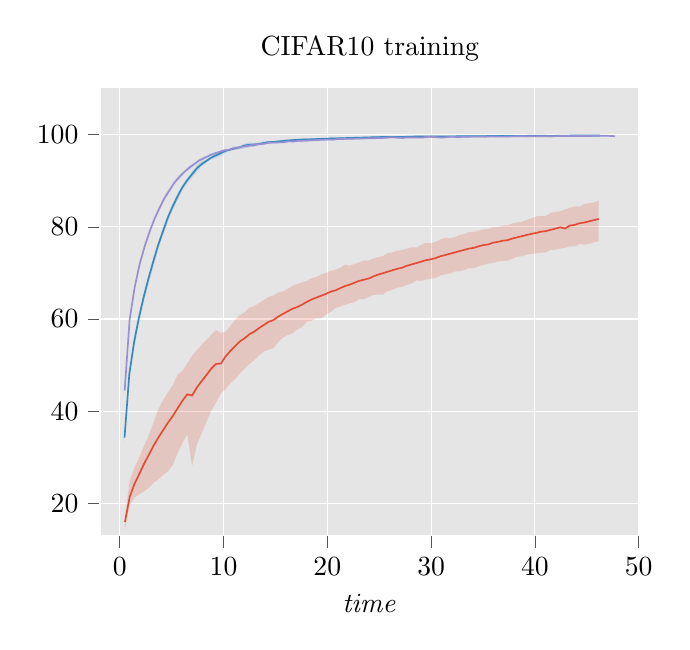
\begin{tikzpicture}

\definecolor{color0}{rgb}{0.886274509803922,0.290196078431373,0.2}
\definecolor{color1}{rgb}{0.203921568627451,0.541176470588235,0.741176470588235}
\definecolor{color2}{rgb}{0.596078431372549,0.556862745098039,0.835294117647059}

\begin{axis}[
axis background/.style={fill=white!89.8039215686275!black},
axis line style={white},
legend cell align={left},
legend style={fill opacity=0.8, draw opacity=1, text opacity=1, at={(0.97,0.03)}, anchor=south east, draw=white!80!black, fill=white!89.8039215686275!black},
log basis y={10},
tick align=outside,
tick pos=left,
title={CIFAR10 training},
x grid style={white},
xlabel={\textit{time}},
xmajorgrids,
xmin=-1.900079335, xmax=50.092281635,
xtick style={color=white!33.3333333333333!black},
y grid style={white},
ymajorgrids,
ymin=12.9249770412146, ymax=110.21669587575,
%ymode=log,
ytick style={color=white!33.3333333333333!black}
]
\path [fill=color0, fill opacity=0.2, very thin]
(axis cs:0.5020421,17.302631)
--(axis cs:0.5020421,14.247533)
--(axis cs:0.963857,19.617599)
--(axis cs:1.4278116,21.28495)
--(axis cs:1.887862,21.942846)
--(axis cs:2.3517187,22.637747)
--(axis cs:2.814011,23.373766)
--(axis cs:3.2743385,24.486019)
--(axis cs:3.7374035,25.21176)
--(axis cs:4.1995907,26.173931)
--(axis cs:4.6610242,26.967516)
--(axis cs:5.1238393,28.400494)
--(axis cs:5.585175,30.908716)
--(axis cs:6.0472547,33.120888)
--(axis cs:6.5086389,35.030838)
--(axis cs:6.9714158,28.116776)
--(axis cs:7.4346022,32.695312)
--(axis cs:7.8944034,35.232319)
--(axis cs:8.3578985,37.637745)
--(axis cs:8.8196617,40.160362)
--(axis cs:9.280207,41.796875)
--(axis cs:9.7445212,43.910362)
--(axis cs:10.20442,44.767681)
--(axis cs:10.6626901,46.025906)
--(axis cs:11.1237508,46.965462)
--(axis cs:11.5831099,48.201069)
--(axis cs:12.0413243,49.276318)
--(axis cs:12.5019929,50.244656)
--(axis cs:12.9604575,51.081413)
--(axis cs:13.419769,52.094982)
--(axis cs:13.8804618,52.9338)
--(axis cs:14.33941,53.347038)
--(axis cs:14.798587,53.630756)
--(axis cs:15.2587694,54.973274)
--(axis cs:15.7175274,55.941612)
--(axis cs:16.177363,56.517269)
--(axis cs:16.6381121,56.85033)
--(axis cs:17.0964306,57.701481)
--(axis cs:17.5551636,58.270969)
--(axis cs:18.0158013,59.405838)
--(axis cs:18.4753143,59.594982)
--(axis cs:18.9333992,60.1213)
--(axis cs:19.3940638,60.115131)
--(axis cs:19.855002,60.910774)
--(axis cs:20.3176195,61.513157)
--(axis cs:20.7764694,62.347862)
--(axis cs:21.2347057,62.726151)
--(axis cs:21.6951497,63.075657)
--(axis cs:22.1549523,63.40255)
--(axis cs:22.6133227,63.643093)
--(axis cs:23.072804,64.278374)
--(axis cs:23.5333105,64.311264)
--(axis cs:23.9920801,64.786186)
--(axis cs:24.4511959,65.232323)
--(axis cs:24.9115622,65.291939)
--(axis cs:25.3712205,65.3125)
--(axis cs:25.8296279,66.017677)
--(axis cs:26.2903579,66.340462)
--(axis cs:26.7499979,66.807152)
--(axis cs:27.2090298,66.967514)
--(axis cs:27.6685594,67.41571)
--(axis cs:28.1287852,67.685036)
--(axis cs:28.5873968,68.384048)
--(axis cs:29.0473541,68.254524)
--(axis cs:29.5077789,68.583473)
--(axis cs:29.9678529,68.731499)
--(axis cs:30.4307062,68.939148)
--(axis cs:30.8959481,69.424339)
--(axis cs:31.3575867,69.681335)
--(axis cs:31.8195534,69.884865)
--(axis cs:32.2810431,70.289886)
--(axis cs:32.7429998,70.38446)
--(axis cs:33.2052788,70.610611)
--(axis cs:33.6670195,71.095802)
--(axis cs:34.1293175,70.970398)
--(axis cs:34.591892,71.426811)
--(axis cs:35.0531397,71.749588)
--(axis cs:35.515564,72.000412)
--(axis cs:35.9772383,72.189552)
--(axis cs:36.4393094,72.493835)
--(axis cs:36.9014965,72.557564)
--(axis cs:37.3627614,72.6912)
--(axis cs:37.8255205,73.044823)
--(axis cs:38.2867267,73.527962)
--(axis cs:38.7492604,73.585526)
--(axis cs:39.210391,73.959702)
--(axis cs:39.6720935,74.089226)
--(axis cs:40.1342356,74.251648)
--(axis cs:40.5967315,74.397614)
--(axis cs:41.0580096,74.424339)
--(axis cs:41.5196336,74.991776)
--(axis cs:41.983765,75.030838)
--(axis cs:42.4478849,75.267273)
--(axis cs:42.9082525,75.437912)
--(axis cs:43.3715823,75.750412)
--(axis cs:43.8334075,75.766861)
--(axis cs:44.2975417,76.276726)
--(axis cs:44.7591353,76.112251)
--(axis cs:45.2199822,76.307564)
--(axis cs:45.6826783,76.659126)
--(axis cs:46.1443844,76.877052)
--(axis cs:46.1443844,85.713402)
--(axis cs:46.1443844,85.713402)
--(axis cs:45.6826783,85.27549)
--(axis cs:45.2199822,85.141861)
--(axis cs:44.7591353,84.969162)
--(axis cs:44.2975417,84.383224)
--(axis cs:43.8334075,84.438736)
--(axis cs:43.3715823,84.115952)
--(axis cs:42.9082525,83.768501)
--(axis cs:42.4478849,83.379936)
--(axis cs:41.983765,83.217514)
--(axis cs:41.5196336,83.00576)
--(axis cs:41.0580096,82.38076)
--(axis cs:40.5967315,82.331413)
--(axis cs:40.1342356,82.27179)
--(axis cs:39.6720935,81.860611)
--(axis cs:39.210391,81.531662)
--(axis cs:38.7492604,81.064964)
--(axis cs:38.2867267,80.945724)
--(axis cs:37.8255205,80.731911)
--(axis cs:37.3627614,80.345398)
--(axis cs:36.9014965,80.289886)
--(axis cs:36.4393094,79.954773)
--(axis cs:35.9772383,79.936264)
--(axis cs:35.515564,79.520973)
--(axis cs:35.0531397,79.465462)
--(axis cs:34.591892,79.196136)
--(axis cs:34.1293175,78.902138)
--(axis cs:33.6670195,78.875412)
--(axis cs:33.2052788,78.408714)
--(axis cs:32.7429998,78.24424)
--(axis cs:32.2810431,77.715874)
--(axis cs:31.8195534,77.567848)
--(axis cs:31.3575867,77.662415)
--(axis cs:30.8959481,77.228615)
--(axis cs:30.4307062,76.737251)
--(axis cs:29.9678529,76.435036)
--(axis cs:29.5077789,76.552223)
--(axis cs:29.0473541,76.106087)
--(axis cs:28.5873968,75.5037)
--(axis cs:28.1287852,75.561264)
--(axis cs:27.6685594,75.300163)
--(axis cs:27.2090298,74.991776)
--(axis cs:26.7499979,74.812912)
--(axis cs:26.2903579,74.428452)
--(axis cs:25.8296279,74.344162)
--(axis cs:25.3712205,73.669823)
--(axis cs:24.9115622,73.392273)
--(axis cs:24.4511959,73.16201)
--(axis cs:23.9920801,72.682976)
--(axis cs:23.5333105,72.662415)
--(axis cs:23.072804,72.323189)
--(axis cs:22.6133227,71.944901)
--(axis cs:22.1549523,71.578949)
--(axis cs:21.6951497,71.7537)
--(axis cs:21.2347057,71.091698)
--(axis cs:20.7764694,70.647614)
--(axis cs:20.3176195,70.411186)
--(axis cs:19.855002,69.987663)
--(axis cs:19.3940638,69.664886)
--(axis cs:18.9333992,69.089226)
--(axis cs:18.4753143,68.861023)
--(axis cs:18.0158013,68.225739)
--(axis cs:17.5551636,67.979027)
--(axis cs:17.0964306,67.574013)
--(axis cs:16.6381121,67.195724)
--(axis cs:16.177363,66.482323)
--(axis cs:15.7175274,65.962173)
--(axis cs:15.2587694,65.740135)
--(axis cs:14.798587,65.115135)
--(axis cs:14.33941,64.798523)
--(axis cs:13.8804618,64.109787)
--(axis cs:13.419769,63.449837)
--(axis cs:12.9604575,62.791943)
--(axis cs:12.5019929,62.495888)
--(axis cs:12.0413243,61.461761)
--(axis cs:11.5831099,60.865543)
--(axis cs:11.1237508,59.769737)
--(axis cs:10.6626901,58.478619)
--(axis cs:10.20442,57.238899)
--(axis cs:9.7445212,56.981907)
--(axis cs:9.280207,57.551399)
--(axis cs:8.8196617,56.591282)
--(axis cs:8.3578985,55.44408)
--(axis cs:7.8944034,54.389393)
--(axis cs:7.4346022,53.188732)
--(axis cs:6.9714158,52.045643)
--(axis cs:6.5086389,50.425575)
--(axis cs:6.0472547,48.772614)
--(axis cs:5.585175,47.956413)
--(axis cs:5.1238393,45.729851)
--(axis cs:4.6610242,44.138569)
--(axis cs:4.1995907,42.458881)
--(axis cs:3.7374035,40.49342)
--(axis cs:3.2743385,37.666531)
--(axis cs:2.814011,34.882812)
--(axis cs:2.3517187,32.532894)
--(axis cs:1.887862,29.94449)
--(axis cs:1.4278116,27.785772)
--(axis cs:0.963857,24.897203)
--(axis cs:0.5020421,17.302631)
--cycle;

\path [fill=color1, fill opacity=0.2, very thin]
(axis cs:0.4632098,35.357731)
--(axis cs:0.4632098,32.94408)
--(axis cs:0.9254774,46.84005)
--(axis cs:1.3881775,53.706825)
--(axis cs:1.8505787,58.96587)
--(axis cs:2.3129487,63.595806)
--(axis cs:2.7754109,67.604851)
--(axis cs:3.2376126,71.313736)
--(axis cs:3.6997682,74.981499)
--(axis cs:4.1622696,78.094162)
--(axis cs:4.6251273,81.011513)
--(axis cs:5.087667,83.71299)
--(axis cs:5.5501337,85.631165)
--(axis cs:6.0128713,87.828949)
--(axis cs:6.475329,89.350327)
--(axis cs:6.9379307,90.612663)
--(axis cs:7.4001751,91.877052)
--(axis cs:7.8623721,93.094162)
--(axis cs:8.3247837,93.836349)
--(axis cs:8.7869458,94.648438)
--(axis cs:9.2494491,94.971214)
--(axis cs:9.7118139,95.355675)
--(axis cs:10.1743406,96.00946)
--(axis cs:10.6367708,96.517273)
--(axis cs:11.0990792,96.665298)
--(axis cs:11.5616002,96.846214)
--(axis cs:12.023917,97.004524)
--(axis cs:12.4861342,97.341698)
--(axis cs:12.9482964,97.368423)
--(axis cs:13.4110369,97.765213)
--(axis cs:13.8734364,97.919411)
--(axis cs:14.3356181,98.098274)
--(axis cs:14.7980995,98.143501)
--(axis cs:15.2603591,98.254524)
--(axis cs:15.7226721,98.194901)
--(axis cs:16.1851398,98.367599)
--(axis cs:16.6474628,98.515625)
--(axis cs:17.109834,98.429276)
--(axis cs:17.5721993,98.527962)
--(axis cs:18.0343757,98.766449)
--(axis cs:18.4972186,98.830177)
--(axis cs:18.9595973,98.928864)
--(axis cs:19.4217701,98.99054)
--(axis cs:19.8841996,98.885689)
--(axis cs:20.3465831,98.838402)
--(axis cs:20.808959,98.969986)
--(axis cs:21.2711594,99.107727)
--(axis cs:21.7335873,98.972038)
--(axis cs:22.1956461,99.064552)
--(axis cs:22.6579044,99.274261)
--(axis cs:23.1202674,99.342102)
--(axis cs:23.5825376,99.309212)
--(axis cs:24.0448372,99.212585)
--(axis cs:24.5074876,99.173523)
--(axis cs:24.9699805,99.444901)
--(axis cs:25.4322128,99.222862)
--(axis cs:25.8946321,99.210526)
--(axis cs:26.3568754,99.375)
--(axis cs:26.8195408,99.395561)
--(axis cs:27.2818438,99.438736)
--(axis cs:27.7444919,99.399673)
--(axis cs:28.2070578,99.444901)
--(axis cs:28.6696802,99.414062)
--(axis cs:29.1318423,99.523026)
--(axis cs:29.594161,99.436676)
--(axis cs:30.0567959,99.377052)
--(axis cs:30.5192224,99.430511)
--(axis cs:30.9818398,99.434624)
--(axis cs:31.4445083,99.29071)
--(axis cs:31.9071473,99.354439)
--(axis cs:32.3696306,99.529198)
--(axis cs:32.8321084,99.483963)
--(axis cs:33.2945942,99.4963)
--(axis cs:33.757296,99.502464)
--(axis cs:34.2195982,99.56826)
--(axis cs:34.6819453,99.584702)
--(axis cs:35.144328,99.547699)
--(axis cs:35.6066388,99.594986)
--(axis cs:36.0693839,99.537415)
--(axis cs:36.5320704,99.533302)
--(axis cs:36.9945851,99.533302)
--(axis cs:37.4569107,99.510689)
--(axis cs:37.9197657,99.605263)
--(axis cs:38.3823447,99.549751)
--(axis cs:38.844871,99.555923)
--(axis cs:39.3072444,99.418175)
--(axis cs:39.7696805,99.609375)
--(axis cs:40.2319381,99.627876)
--(axis cs:40.6940758,99.590874)
--(axis cs:41.1565834,99.451073)
--(axis cs:41.6190216,99.335938)
--(axis cs:42.0813775,99.570312)
--(axis cs:42.5436282,99.683388)
--(axis cs:43.0058633,99.72451)
--(axis cs:43.4683882,99.743011)
--(axis cs:43.930484,99.765625)
--(axis cs:44.3925875,99.72451)
--(axis cs:44.8548618,99.749176)
--(axis cs:45.3173953,99.72451)
--(axis cs:45.7795459,99.625824)
--(axis cs:46.2420028,99.486023)
--(axis cs:46.2420028,99.909538)
--(axis cs:46.2420028,99.909538)
--(axis cs:45.7795459,99.925987)
--(axis cs:45.3173953,99.905426)
--(axis cs:44.8548618,99.899261)
--(axis cs:44.3925875,99.905426)
--(axis cs:43.930484,99.845802)
--(axis cs:43.4683882,99.907486)
--(axis cs:43.0058633,99.884865)
--(axis cs:42.5436282,99.911598)
--(axis cs:42.0813775,99.901314)
--(axis cs:41.6190216,99.917763)
--(axis cs:41.1565834,99.882812)
--(axis cs:40.6940758,99.841698)
--(axis cs:40.2319381,99.868423)
--(axis cs:39.7696805,99.92804)
--(axis cs:39.3072444,99.854027)
--(axis cs:38.844871,99.891037)
--(axis cs:38.3823447,99.91571)
--(axis cs:37.9197657,99.882812)
--(axis cs:37.4569107,99.8787)
--(axis cs:36.9945851,99.837585)
--(axis cs:36.5320704,99.845802)
--(axis cs:36.0693839,99.860199)
--(axis cs:35.6066388,99.901314)
--(axis cs:35.144328,99.872536)
--(axis cs:34.6819453,99.899261)
--(axis cs:34.2195982,99.866364)
--(axis cs:33.757296,99.794411)
--(axis cs:33.2945942,99.868423)
--(axis cs:32.8321084,99.821136)
--(axis cs:32.3696306,99.851974)
--(axis cs:31.9071473,99.769737)
--(axis cs:31.4445083,99.794411)
--(axis cs:30.9818398,99.765625)
--(axis cs:30.5192224,99.788239)
--(axis cs:30.0567959,99.792351)
--(axis cs:29.594161,99.701889)
--(axis cs:29.1318423,99.72245)
--(axis cs:28.6696802,99.802635)
--(axis cs:28.2070578,99.786186)
--(axis cs:27.7444919,99.677223)
--(axis cs:27.2818438,99.65255)
--(axis cs:26.8195408,99.601151)
--(axis cs:26.3568754,99.636101)
--(axis cs:25.8946321,99.679276)
--(axis cs:25.4322128,99.736839)
--(axis cs:24.9699805,99.658714)
--(axis cs:24.5074876,99.668999)
--(axis cs:24.0448372,99.578537)
--(axis cs:23.5825376,99.560036)
--(axis cs:23.1202674,99.512749)
--(axis cs:22.6579044,99.597038)
--(axis cs:22.1956461,99.471626)
--(axis cs:21.7335873,99.387337)
--(axis cs:21.2711594,99.426399)
--(axis cs:20.808959,99.527138)
--(axis cs:20.3465831,99.518913)
--(axis cs:19.8841996,99.300987)
--(axis cs:19.4217701,99.187912)
--(axis cs:18.9595973,99.257812)
--(axis cs:18.4972186,99.120064)
--(axis cs:18.0343757,99.226974)
--(axis cs:17.5721993,99.115952)
--(axis cs:17.109834,99.107727)
--(axis cs:16.6474628,99.126236)
--(axis cs:16.1851398,98.951477)
--(axis cs:15.7226721,98.850739)
--(axis cs:15.2603591,98.830177)
--(axis cs:14.7980995,98.620476)
--(axis cs:14.3356181,98.599915)
--(axis cs:13.8734364,98.546463)
--(axis cs:13.4110369,98.273026)
--(axis cs:12.9482964,98.106499)
--(axis cs:12.4861342,98.279198)
--(axis cs:12.023917,97.995476)
--(axis cs:11.5616002,97.481499)
--(axis cs:11.0990792,97.329361)
--(axis cs:10.6367708,96.940788)
--(axis cs:10.1743406,96.83799)
--(axis cs:9.7118139,96.416527)
--(axis cs:9.2494491,95.727798)
--(axis cs:8.7869458,95.302223)
--(axis cs:8.3247837,94.607323)
--(axis cs:7.8623721,94.220802)
--(axis cs:7.4001751,93.250412)
--(axis cs:6.9379307,91.920227)
--(axis cs:6.475329,90.462585)
--(axis cs:6.0128713,88.895973)
--(axis cs:5.5501337,87.15049)
--(axis cs:5.087667,85.018501)
--(axis cs:4.6251273,82.411598)
--(axis cs:4.1622696,79.658714)
--(axis cs:3.6997682,76.652962)
--(axis cs:3.2376126,73.131165)
--(axis cs:2.7754109,69.551811)
--(axis cs:2.3129487,65.701073)
--(axis cs:1.8505787,61.235607)
--(axis cs:1.3881775,56.145149)
--(axis cs:0.9254774,49.03783)
--(axis cs:0.4632098,35.357731)
--cycle;

\path [fill=color2, fill opacity=0.2, very thin]
(axis cs:0.4787409,45.032895)
--(axis cs:0.4787409,43.869243)
--(axis cs:0.9549568,59.272204)
--(axis cs:1.4328986,66.276727)
--(axis cs:1.9128344,71.284951)
--(axis cs:2.3927933,75.279605)
--(axis cs:2.875019,78.591694)
--(axis cs:3.3514207,81.449424)
--(axis cs:3.8258368,83.554688)
--(axis cs:4.3021816,85.797697)
--(axis cs:4.7785431,87.553454)
--(axis cs:5.2544502,89.159128)
--(axis cs:5.7327906,90.390625)
--(axis cs:6.2106256,91.599507)
--(axis cs:6.6934447,92.395148)
--(axis cs:7.1764946,93.151727)
--(axis cs:7.6527392,94.130345)
--(axis cs:8.1276748,94.627878)
--(axis cs:8.6052351,95.20148)
--(axis cs:9.0833687,95.723684)
--(axis cs:9.5603715,95.908717)
--(axis cs:10.0355231,96.340461)
--(axis cs:10.5112275,96.410362)
--(axis cs:10.9890443,96.833882)
--(axis cs:11.4700498,96.942845)
--(axis cs:11.9460153,97.189556)
--(axis cs:12.4240194,97.203947)
--(axis cs:12.9025472,97.341694)
--(axis cs:13.3790138,97.703536)
--(axis cs:13.8546063,97.76727)
--(axis cs:14.3295909,98.050987)
--(axis cs:14.8081463,97.993421)
--(axis cs:15.289785,98.133224)
--(axis cs:15.7659315,98.159951)
--(axis cs:16.2408114,98.414885)
--(axis cs:16.7177102,98.221628)
--(axis cs:17.1941908,98.408717)
--(axis cs:17.6725458,98.223684)
--(axis cs:18.153403,98.406661)
--(axis cs:18.631386,98.60403)
--(axis cs:19.1072212,98.534128)
--(axis cs:19.5814395,98.809622)
--(axis cs:20.0587741,98.690378)
--(axis cs:20.5357722,98.729441)
--(axis cs:21.0118284,98.926809)
--(axis cs:21.4875376,98.96176)
--(axis cs:21.9662875,98.834293)
--(axis cs:22.4450026,98.957648)
--(axis cs:22.921241,98.945312)
--(axis cs:23.3970977,98.957648)
--(axis cs:23.8751955,99.091283)
--(axis cs:24.3509275,99.060444)
--(axis cs:24.8275496,99.023438)
--(axis cs:25.3055867,99.081003)
--(axis cs:25.784609,99.187911)
--(axis cs:26.26137,99.204359)
--(axis cs:26.7373334,99.085115)
--(axis cs:27.2131395,99.054276)
--(axis cs:27.6884838,99.171464)
--(axis cs:28.1644315,99.255757)
--(axis cs:28.6431342,99.175576)
--(axis cs:29.1211952,99.115954)
--(axis cs:29.597205,99.31949)
--(axis cs:30.074211,99.379112)
--(axis cs:30.5499029,99.249589)
--(axis cs:31.0274016,99.216694)
--(axis cs:31.5027262,99.368832)
--(axis cs:31.9795899,99.424342)
--(axis cs:32.4580046,99.245477)
--(axis cs:32.9333126,99.463405)
--(axis cs:33.4104359,99.358553)
--(axis cs:33.8869678,99.379112)
--(axis cs:34.3650765,99.32977)
--(axis cs:34.8432337,99.288651)
--(axis cs:35.3232167,99.399671)
--(axis cs:35.8059391,99.391447)
--(axis cs:36.2872295,99.38528)
--(axis cs:36.763833,99.409951)
--(axis cs:37.2396782,99.481908)
--(axis cs:37.7172186,99.451069)
--(axis cs:38.1930911,99.453125)
--(axis cs:38.6720442,99.481908)
--(axis cs:39.1488671,99.426398)
--(axis cs:39.6243587,99.479852)
--(axis cs:40.0995631,99.580592)
--(axis cs:40.5750744,99.488076)
--(axis cs:41.0521059,99.500411)
--(axis cs:41.5299999,99.506579)
--(axis cs:42.0052569,99.539474)
--(axis cs:42.4803443,99.457237)
--(axis cs:42.9563098,99.572368)
--(axis cs:43.4326693,99.601151)
--(axis cs:43.9082268,99.537418)
--(axis cs:44.3837151,99.465461)
--(axis cs:44.8605593,99.599095)
--(axis cs:45.340364,99.580592)
--(axis cs:45.8189316,99.599095)
--(axis cs:46.296049,99.603207)
--(axis cs:46.7714856,99.597039)
--(axis cs:47.2480983,99.494243)
--(axis cs:47.7289925,99.393503)
--(axis cs:47.7289925,99.796464)
--(axis cs:47.7289925,99.796464)
--(axis cs:47.2480983,99.817023)
--(axis cs:46.7714856,99.897204)
--(axis cs:46.296049,99.932155)
--(axis cs:45.8189316,99.913651)
--(axis cs:45.340364,99.971217)
--(axis cs:44.8605593,99.936266)
--(axis cs:44.3837151,99.985609)
--(axis cs:43.9082268,99.962993)
--(axis cs:43.4326693,99.85403)
--(axis cs:42.9563098,99.749178)
--(axis cs:42.4803443,99.872533)
--(axis cs:42.0052569,99.872533)
--(axis cs:41.5299999,99.812911)
--(axis cs:41.0521059,99.773849)
--(axis cs:40.5750744,99.817023)
--(axis cs:40.0995631,99.769737)
--(axis cs:39.6243587,99.79852)
--(axis cs:39.1488671,99.800576)
--(axis cs:38.6720442,99.79852)
--(axis cs:38.1930911,99.819079)
--(axis cs:37.7172186,99.810855)
--(axis cs:37.2396782,99.691612)
--(axis cs:36.763833,99.747122)
--(axis cs:36.2872295,99.777961)
--(axis cs:35.8059391,99.755345)
--(axis cs:35.3232167,99.784128)
--(axis cs:34.8432337,99.753289)
--(axis cs:34.3650765,99.73273)
--(axis cs:33.8869678,99.724507)
--(axis cs:33.4104359,99.738898)
--(axis cs:32.9333126,99.601151)
--(axis cs:32.4580046,99.621711)
--(axis cs:31.9795899,99.699836)
--(axis cs:31.5027262,99.564145)
--(axis cs:31.0274016,99.469572)
--(axis cs:30.5499029,99.738898)
--(axis cs:30.074211,99.685444)
--(axis cs:29.597205,99.675164)
--(axis cs:29.1211952,99.535362)
--(axis cs:28.6431342,99.551809)
--(axis cs:28.1644315,99.483964)
--(axis cs:27.6884838,99.539474)
--(axis cs:27.2131395,99.537418)
--(axis cs:26.7373334,99.502467)
--(axis cs:26.26137,99.597039)
--(axis cs:25.784609,99.572368)
--(axis cs:25.3055867,99.555921)
--(axis cs:24.8275496,99.494243)
--(axis cs:24.3509275,99.465461)
--(axis cs:23.8751955,99.481908)
--(axis cs:23.3970977,99.405839)
--(axis cs:22.921241,99.294819)
--(axis cs:22.4450026,99.294819)
--(axis cs:21.9662875,99.325658)
--(axis cs:21.4875376,99.239309)
--(axis cs:21.0118284,99.247533)
--(axis cs:20.5357722,99.081003)
--(axis cs:20.0587741,99.095395)
--(axis cs:19.5814395,99.305099)
--(axis cs:19.1072212,99.103618)
--(axis cs:18.631386,98.974095)
--(axis cs:18.153403,99.103618)
--(axis cs:17.6725458,98.996711)
--(axis cs:17.1941908,98.937089)
--(axis cs:16.7177102,98.735609)
--(axis cs:16.2408114,98.766447)
--(axis cs:15.7659315,98.474507)
--(axis cs:15.289785,98.375822)
--(axis cs:14.8081463,98.4375)
--(axis cs:14.3295909,98.562911)
--(axis cs:13.8546063,98.363487)
--(axis cs:13.3790138,98.196957)
--(axis cs:12.9025472,98.196957)
--(axis cs:12.4240194,97.870066)
--(axis cs:11.9460153,97.691201)
--(axis cs:11.4700498,97.514391)
--(axis cs:10.9890443,97.450658)
--(axis cs:10.5112275,96.942845)
--(axis cs:10.0355231,96.700247)
--(axis cs:9.5603715,96.480263)
--(axis cs:9.0833687,96.04852)
--(axis cs:8.6052351,95.740132)
--(axis cs:8.1276748,95.219984)
--(axis cs:7.6527392,94.827303)
--(axis cs:7.1764946,93.840461)
--(axis cs:6.6934447,93.211349)
--(axis cs:6.2106256,92.066201)
--(axis cs:5.7327906,91.352796)
--(axis cs:5.2544502,90.006168)
--(axis cs:4.7785431,88.342928)
--(axis cs:4.3021816,86.661184)
--(axis cs:3.8258368,84.537418)
--(axis cs:3.3514207,82.105263)
--(axis cs:2.875019,79.48602)
--(axis cs:2.3927933,76.585115)
--(axis cs:1.9128344,72.448602)
--(axis cs:1.4328986,67.754934)
--(axis cs:0.9549568,60.474918)
--(axis cs:0.4787409,45.032895)
--cycle;

\addplot [semithick, color0]
table {%
0.502042055130005 15.9457235336304
0.963856935501099 21.4037857055664
1.42781162261963 24.243631362915
1.88786196708679 26.3706817626953
2.35171866416931 28.6122512817383
2.81401109695435 30.5713405609131
3.27433848381042 32.5567436218262
3.73740339279175 34.3186683654785
4.66102409362793 37.5427589416504
5.12383937835693 38.9617652893066
5.58517503738403 40.6632347106934
6.04725456237793 42.2781677246094
6.50863885879517 43.6554298400879
6.97141599655151 43.3858909606934
7.4346022605896 45.1305541992188
7.8944034576416 46.5248794555664
8.3578987121582 47.8418960571289
8.81966209411621 49.2319107055664
9.28020668029785 50.2534942626953
9.74452114105225 50.3205223083496
10.2044200897217 51.8789100646973
10.6626901626587 53.0625
11.5831098556519 55.1548194885254
12.0413246154785 55.8285331726074
12.5019931793213 56.702507019043
12.9604578018188 57.2481536865234
13.4197692871094 58.0203475952148
14.339409828186 59.3741760253906
14.7985868453979 59.7549285888672
15.2587690353394 60.4963073730469
16.1773624420166 61.6687889099121
16.6381130218506 62.2047729492188
17.0964298248291 62.5999183654785
17.5551643371582 63.0918998718262
18.0158004760742 63.7064094543457
18.4753150939941 64.2308883666992
19.855001449585 65.4292678833008
20.3176193237305 65.9309234619141
20.7764701843262 66.2018890380859
21.6951503753662 67.1377487182617
22.1549530029297 67.4483947753906
23.0728034973145 68.2808380126953
23.9920806884766 68.7816619873047
24.4511966705322 69.253288269043
24.9115619659424 69.6328201293945
26.7499980926514 70.9007034301758
27.2090301513672 71.1223297119141
27.6685600280762 71.5534515380859
28.5873966217041 72.1330261230469
29.5077781677246 72.7606811523438
29.9678535461426 72.9461364746094
30.4307060241699 73.2142333984375
30.8959484100342 73.600944519043
33.6670188903809 75.2919311523438
34.1293182373047 75.4430541992188
34.5918922424316 75.7818756103516
35.0531387329102 76.0501708984375
35.5155639648438 76.1729049682617
35.977237701416 76.5668182373047
36.4393081665039 76.7436218261719
36.901496887207 76.9808731079102
37.3627624511719 77.1015548706055
37.8255195617676 77.4597091674805
39.6720924377441 78.4806823730469
40.1342353820801 78.6733093261719
40.5967330932617 78.947151184082
41.0580101013184 79.0719680786133
42.447883605957 79.8916625976562
42.9082527160645 79.6194381713867
43.37158203125 80.2878341674805
43.8334083557129 80.4111862182617
44.2975425720215 80.7754898071289
44.7591361999512 80.9325561523438
46.1443862915039 81.7109375
};
%\addlegendentry{cudnn}
\addplot [semithick, color1]
table {%
0.463209867477417 34.242603302002
0.925477385520935 48.0653877258301
1.38817751407623 55.0246696472168
1.85057866573334 60.2843284606934
2.31294870376587 64.8098297119141
2.77541089057922 68.8412933349609
3.23761248588562 72.5045318603516
3.69976830482483 76.0178833007812
4.16226959228516 79.0146026611328
4.62512731552124 81.9558029174805
5.0876669883728 84.3402557373047
5.55013370513916 86.5086441040039
6.01287126541138 88.4905548095703
6.47532892227173 90.0304336547852
7.40017509460449 92.6173934936523
7.86237192153931 93.5476989746094
8.78694534301758 94.9656600952148
9.24944877624512 95.4919738769531
10.1743402481079 96.4671173095703
11.0990791320801 97.0131759643555
11.5615997314453 97.2576141357422
12.0239171981812 97.6519393920898
12.4861345291138 97.7910995483398
12.948296546936 97.7999649047852
14.335618019104 98.3737564086914
14.7980995178223 98.4019241333008
16.1851406097412 98.7345809936523
17.5721988677979 98.9352569580078
18.4972190856934 98.995475769043
19.4217700958252 99.0933532714844
25.4322128295898 99.4987487792969
27.2818431854248 99.5119171142578
29.1318416595459 99.6276626586914
30.0567951202393 99.5908584594727
36.5320701599121 99.7105331420898
37.4569091796875 99.6967620849609
40.2319374084473 99.7691192626953
41.6190223693848 99.7312774658203
43.9304847717285 99.8192749023438
45.7795448303223 99.8199081420898
46.2420043945312 99.8166198730469
};
%\addlegendentry{libtorch}
\addplot [semithick, color2]
table {%
0.478740930557251 44.5092468261719
0.954956769943237 59.8593711853027
1.43289864063263 66.7787780761719
1.91283440589905 71.8283386230469
2.39279341697693 75.6295166015625
2.87501907348633 78.9113845825195
3.35142064094543 81.7136077880859
3.82583689689636 84.0302200317383
4.30218172073364 86.1776275634766
5.25445032119751 89.5509796142578
5.73279047012329 90.7748870849609
6.21062564849854 91.8698577880859
6.69344472885132 92.8338928222656
7.65273904800415 94.3871231079102
8.60523509979248 95.4331741333008
9.0833683013916 95.8809585571289
10.0355234146118 96.5851287841797
10.5112276077271 96.7082748413086
10.9890441894531 97.0834732055664
11.4700498580933 97.2029342651367
11.9460153579712 97.453125
12.4240198135376 97.5894241333008
12.9025468826294 97.8538284301758
13.854606628418 98.0008316040039
14.3295907974243 98.2436370849609
15.7659311294556 98.3449783325195
16.2408123016357 98.5549011230469
16.7177104949951 98.5191116333008
17.1941909790039 98.6562576293945
20.0587749481201 98.9375076293945
20.5357723236084 98.909538269043
21.0118274688721 99.0386428833008
25.3055858612061 99.2777481079102
26.2613697052002 99.4350280761719
27.2131385803223 99.2769317626953
27.6884841918945 99.4001007080078
28.6431350708008 99.3663558959961
29.1211948394775 99.3548431396484
29.597204208374 99.4985580444336
30.0742111206055 99.5378189086914
31.027400970459 99.3470458984375
31.9795894622803 99.5707168579102
32.4580039978027 99.4773941040039
33.8869667053223 99.5703048706055
35.3232154846191 99.5598373413086
35.8059387207031 99.6256103515625
36.7638320922852 99.5594329833984
38.1930923461914 99.6453552246094
41.0521049499512 99.6420745849609
42.4803428649902 99.7004623413086
44.383716583252 99.6891555786133
46.771484375 99.772216796875
47.7289924621582 99.6677627563477
};
%\addlegendentry{pytorch}
\end{axis}

\end{tikzpicture}

    \end{figure}


    \begin{figure}
        % This file was created by tikzplotlib v0.9.5.
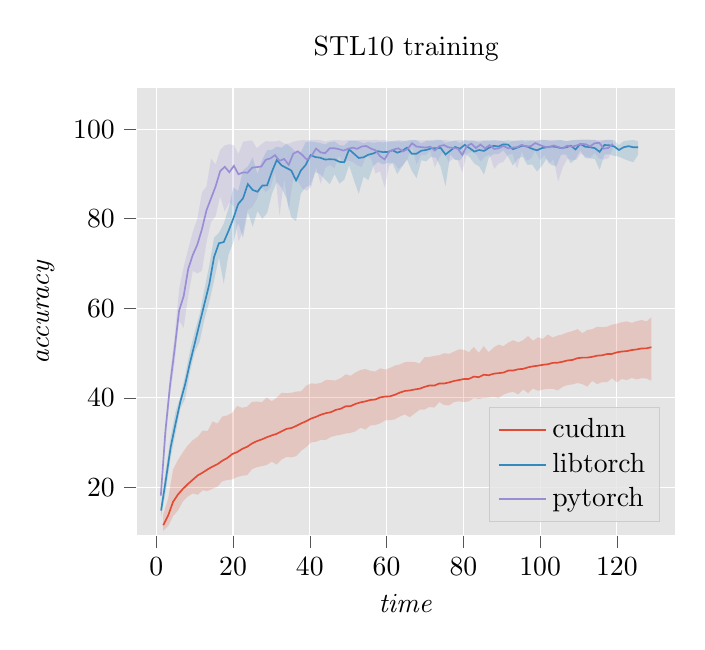
\begin{tikzpicture}

\definecolor{color0}{rgb}{0.886274509803922,0.290196078431373,0.2}
\definecolor{color1}{rgb}{0.203921568627451,0.541176470588235,0.741176470588235}
\definecolor{color2}{rgb}{0.596078431372549,0.556862745098039,0.835294117647059}

\begin{axis}[
axis background/.style={fill=white!89.8039215686275!black},
axis line style={white},
legend cell align={left},
legend style={fill opacity=0.8, draw opacity=1, text opacity=1, at={(0.97,0.03)}, anchor=south east, draw=white!80!black, fill=white!89.8039215686275!black},
log basis y={10},
tick align=outside,
tick pos=left,
title={STL10 training},
x grid style={white},
xlabel={\textit{time}},
xmajorgrids,
xmin=-5.19760163, xmax=135.38068523,
xtick style={color=white!33.3333333333333!black},
y grid style={white},
ylabel={\textit{accuracy}},
ymajorgrids,
ymin=9.14280358979306, ymax=109.315558819346,
%ymode=log,
ytick style={color=white!33.3333333333333!black}
]
\path [fill=color0, fill opacity=0.2, very thin]
(axis cs:1.8181475,13.919271)
--(axis cs:1.8181475,10.234375)
--(axis cs:3.1015922,11.341146)
--(axis cs:4.3881964,13.541667)
--(axis cs:5.6697498,14.817708)
--(axis cs:6.9567745,16.848959)
--(axis cs:8.2428672,17.942709)
--(axis cs:9.5269492,18.619791)
--(axis cs:10.8122282,18.333334)
--(axis cs:12.0991791,19.322916)
--(axis cs:13.3812914,19.166666)
--(axis cs:14.6654891,19.661459)
--(axis cs:15.9478969,20.195312)
--(axis cs:17.232328,21.354166)
--(axis cs:18.5146575,21.640625)
--(axis cs:19.8012213,21.744791)
--(axis cs:21.0840842,22.304688)
--(axis cs:22.3683458,22.591146)
--(axis cs:23.651952,22.708334)
--(axis cs:24.9376781,24.023438)
--(axis cs:26.2201795,24.505209)
--(axis cs:27.5038189,24.713541)
--(axis cs:28.7885163,24.973959)
--(axis cs:30.0761489,25.742188)
--(axis cs:31.358376,25.065104)
--(axis cs:32.6423435,26.210938)
--(axis cs:33.9274175,26.770834)
--(axis cs:35.2126796,26.692709)
--(axis cs:36.4976855,26.953125)
--(axis cs:37.7835537,28.190104)
--(axis cs:39.0670015,28.971354)
--(axis cs:40.3503277,30.039062)
--(axis cs:41.6357876,30.182291)
--(axis cs:42.9215691,30.598959)
--(axis cs:44.2048227,30.598959)
--(axis cs:45.490117,31.25)
--(axis cs:46.7742425,31.549479)
--(axis cs:48.0608687,31.744791)
--(axis cs:49.3439484,32.005207)
--(axis cs:50.628987,32.161457)
--(axis cs:51.9142668,32.5)
--(axis cs:53.1983139,33.320312)
--(axis cs:54.4834733,32.903645)
--(axis cs:55.7678699,33.815105)
--(axis cs:57.0510268,33.91927)
--(axis cs:58.3349453,34.270832)
--(axis cs:59.6192652,34.947918)
--(axis cs:60.9042402,35.01302)
--(axis cs:62.1854784,35.182293)
--(axis cs:63.4683535,35.833332)
--(axis cs:64.7523611,36.289062)
--(axis cs:66.0399125,35.651043)
--(axis cs:67.3233237,36.484375)
--(axis cs:68.6089274,37.33073)
--(axis cs:69.8913879,37.382812)
--(axis cs:71.1745869,37.942707)
--(axis cs:72.4576266,37.8125)
--(axis cs:73.7439566,39.0625)
--(axis cs:75.0281581,38.346355)
--(axis cs:76.3165164,38.320312)
--(axis cs:77.5979577,39.0625)
--(axis cs:78.8851048,39.192707)
--(axis cs:80.1680884,39.0625)
--(axis cs:81.4541719,39.192707)
--(axis cs:82.738797,39.973957)
--(axis cs:84.0242694,39.726562)
--(axis cs:85.3116352,39.934895)
--(axis cs:86.5965253,40.039062)
--(axis cs:87.8830559,40.182293)
--(axis cs:89.1684826,39.947918)
--(axis cs:90.451034,40.690105)
--(axis cs:91.7357714,41.132812)
--(axis cs:93.0172198,41.315105)
--(axis cs:94.3033933,40.742188)
--(axis cs:95.5860217,41.835938)
--(axis cs:96.8740081,41.041668)
--(axis cs:98.1589983,42.070312)
--(axis cs:99.4438364,41.5625)
--(axis cs:100.726415,41.835938)
--(axis cs:102.009401,42.005207)
--(axis cs:103.2938186,42.005207)
--(axis cs:104.5794376,41.653645)
--(axis cs:105.8616588,42.434895)
--(axis cs:107.1464607,42.851562)
--(axis cs:108.4291424,42.98177)
--(axis cs:109.7167975,43.307293)
--(axis cs:111.0016509,43.046875)
--(axis cs:112.2889483,42.5)
--(axis cs:113.5706432,43.76302)
--(axis cs:114.855097,43.059895)
--(axis cs:116.1407626,43.502605)
--(axis cs:117.4265288,43.463543)
--(axis cs:118.7118835,44.38802)
--(axis cs:119.9955895,43.463543)
--(axis cs:121.2795428,44.192707)
--(axis cs:122.567516,43.945312)
--(axis cs:123.8486356,44.440105)
--(axis cs:125.1355257,44.101562)
--(axis cs:126.4196376,44.38802)
--(axis cs:127.7084405,44.296875)
--(axis cs:128.9907631,43.802082)
--(axis cs:128.9907631,58.007812)
--(axis cs:128.9907631,58.007812)
--(axis cs:127.7084405,57.057293)
--(axis cs:126.4196376,57.382812)
--(axis cs:125.1355257,57.122395)
--(axis cs:123.8486356,56.744793)
--(axis cs:122.567516,57.070312)
--(axis cs:121.2795428,56.875)
--(axis cs:119.9955895,56.5625)
--(axis cs:118.7118835,56.328125)
--(axis cs:117.4265288,55.898438)
--(axis cs:116.1407626,55.755207)
--(axis cs:114.855097,55.885418)
--(axis cs:113.5706432,55.338543)
--(axis cs:112.2889483,55.14323)
--(axis cs:111.0016509,54.427082)
--(axis cs:109.7167975,55.351562)
--(axis cs:108.4291424,54.882812)
--(axis cs:107.1464607,54.609375)
--(axis cs:105.8616588,54.166668)
--(axis cs:104.5794376,53.91927)
--(axis cs:103.2938186,53.463543)
--(axis cs:102.009401,54.140625)
--(axis cs:100.726415,53.164062)
--(axis cs:99.4438364,53.515625)
--(axis cs:98.1589983,52.747395)
--(axis cs:96.8740081,53.815105)
--(axis cs:95.5860217,52.890625)
--(axis cs:94.3033933,52.382812)
--(axis cs:93.0172198,52.864582)
--(axis cs:91.7357714,52.35677)
--(axis cs:90.451034,51.54948)
--(axis cs:89.1684826,51.88802)
--(axis cs:87.8830559,51.23698)
--(axis cs:86.5965253,50.182293)
--(axis cs:85.3116352,51.54948)
--(axis cs:84.0242694,50.039062)
--(axis cs:82.738797,51.341145)
--(axis cs:81.4541719,50.208332)
--(axis cs:80.1680884,50.716145)
--(axis cs:78.8851048,50.833332)
--(axis cs:77.5979577,50.338543)
--(axis cs:76.3165164,49.83073)
--(axis cs:75.0281581,49.960938)
--(axis cs:73.7439566,49.51823)
--(axis cs:72.4576266,49.36198)
--(axis cs:71.1745869,49.140625)
--(axis cs:69.8913879,49.07552)
--(axis cs:68.6089274,47.65625)
--(axis cs:67.3233237,47.994793)
--(axis cs:66.0399125,48.046875)
--(axis cs:64.7523611,47.96875)
--(axis cs:63.4683535,47.447918)
--(axis cs:62.1854784,47.20052)
--(axis cs:60.9042402,46.666668)
--(axis cs:59.6192652,46.302082)
--(axis cs:58.3349453,46.57552)
--(axis cs:57.0510268,45.885418)
--(axis cs:55.7678699,46.028645)
--(axis cs:54.4834733,46.432293)
--(axis cs:53.1983139,46.223957)
--(axis cs:51.9142668,45.677082)
--(axis cs:50.628987,44.934895)
--(axis cs:49.3439484,45.234375)
--(axis cs:48.0608687,44.401043)
--(axis cs:46.7742425,43.89323)
--(axis cs:45.490117,43.932293)
--(axis cs:44.2048227,43.997395)
--(axis cs:42.9215691,43.320312)
--(axis cs:41.6357876,43.151043)
--(axis cs:40.3503277,43.216145)
--(axis cs:39.0670015,42.708332)
--(axis cs:37.7835537,41.471355)
--(axis cs:36.4976855,41.39323)
--(axis cs:35.2126796,41.119793)
--(axis cs:33.9274175,41.028645)
--(axis cs:32.6423435,41.119793)
--(axis cs:31.358376,40)
--(axis cs:30.0761489,39.23177)
--(axis cs:28.7885163,40.065105)
--(axis cs:27.5038189,38.984375)
--(axis cs:26.2201795,39.179688)
--(axis cs:24.9376781,39.04948)
--(axis cs:23.651952,38.007812)
--(axis cs:22.3683458,37.760418)
--(axis cs:21.0840842,38.177082)
--(axis cs:19.8012213,36.666668)
--(axis cs:18.5146575,36.067707)
--(axis cs:17.232328,35.833332)
--(axis cs:15.9478969,34.244793)
--(axis cs:14.6654891,34.739582)
--(axis cs:13.3812914,32.578125)
--(axis cs:12.0991791,32.682293)
--(axis cs:10.8122282,31.289062)
--(axis cs:9.5269492,30.546875)
--(axis cs:8.2428672,29.388021)
--(axis cs:6.9567745,27.851562)
--(axis cs:5.6697498,26.119791)
--(axis cs:4.3881964,23.997396)
--(axis cs:3.1015922,17.486979)
--(axis cs:1.8181475,13.919271)
--cycle;

\path [fill=color1, fill opacity=0.2, very thin]
(axis cs:1.2572434,16.328125)
--(axis cs:1.2572434,13.339844)
--(axis cs:2.5172312,19.179688)
--(axis cs:3.7711002,26.796875)
--(axis cs:5.022725,31.972656)
--(axis cs:6.2778645,37.636719)
--(axis cs:7.5325557,39.746094)
--(axis cs:8.7884026,45.800781)
--(axis cs:10.0442825,50.234375)
--(axis cs:11.3001487,52.519531)
--(axis cs:12.5558317,57.539062)
--(axis cs:13.813037,61.445312)
--(axis cs:15.0695192,66.230469)
--(axis cs:16.3259816,71.367188)
--(axis cs:17.581719,65.507812)
--(axis cs:18.8377473,71.992188)
--(axis cs:20.0918182,74.824219)
--(axis cs:21.3473531,79.0625)
--(axis cs:22.603765,75.722656)
--(axis cs:23.861623,81.503906)
--(axis cs:25.1170369,78.242188)
--(axis cs:26.3717957,81.738281)
--(axis cs:27.6281248,79.960938)
--(axis cs:28.8846523,81.289062)
--(axis cs:30.1416594,85.566406)
--(axis cs:31.3969638,88.222656)
--(axis cs:32.6534027,86.914062)
--(axis cs:33.9101459,84.609375)
--(axis cs:35.1660355,80.292969)
--(axis cs:36.422017,79.472656)
--(axis cs:37.6763219,85.644531)
--(axis cs:38.931803,87.011719)
--(axis cs:40.1894583,87.578125)
--(axis cs:41.446448,90.429688)
--(axis cs:42.7027211,89.960938)
--(axis cs:43.9562373,88.808594)
--(axis cs:45.2120456,87.734375)
--(axis cs:46.4665121,89.980469)
--(axis cs:47.7242048,87.851562)
--(axis cs:48.9775083,88.710938)
--(axis cs:50.2334429,91.933594)
--(axis cs:51.4900184,88.671875)
--(axis cs:52.745522,85.585938)
--(axis cs:53.9997774,89.394531)
--(axis cs:55.2561939,88.632812)
--(axis cs:56.5128563,91.757812)
--(axis cs:57.7700699,92.714844)
--(axis cs:59.0265381,92.148438)
--(axis cs:60.2807585,92.460938)
--(axis cs:61.5355289,92.421875)
--(axis cs:62.7895891,89.980469)
--(axis cs:64.0442244,91.679688)
--(axis cs:65.3006613,93.28125)
--(axis cs:66.5541206,90.742188)
--(axis cs:67.8099738,89.042969)
--(axis cs:69.0641438,93.085938)
--(axis cs:70.3209835,92.8125)
--(axis cs:71.5770803,93.847656)
--(axis cs:72.83228,93.671875)
--(axis cs:74.0878983,91.621094)
--(axis cs:75.3433888,87.265625)
--(axis cs:76.5951476,94.355469)
--(axis cs:77.8479253,93.183594)
--(axis cs:79.1027417,93.046875)
--(axis cs:80.3586953,94.550781)
--(axis cs:81.6110766,93.808594)
--(axis cs:82.866656,92.34375)
--(axis cs:84.122545,91.699219)
--(axis cs:85.378461,89.84375)
--(axis cs:86.6355466,93.691406)
--(axis cs:87.8884647,94.433594)
--(axis cs:89.1453755,94.433594)
--(axis cs:90.4002351,95.273438)
--(axis cs:91.6575148,93.828125)
--(axis cs:92.9107424,91.894531)
--(axis cs:94.1655439,93.378906)
--(axis cs:95.4185916,93.886719)
--(axis cs:96.6754833,92.03125)
--(axis cs:97.9307792,92.128906)
--(axis cs:99.1860832,90.566406)
--(axis cs:100.4418415,91.777344)
--(axis cs:101.6954069,93.4375)
--(axis cs:102.9511175,91.992188)
--(axis cs:104.2052924,91.777344)
--(axis cs:105.4607916,94.296875)
--(axis cs:106.7130088,94.335938)
--(axis cs:107.9684443,92.421875)
--(axis cs:109.2243049,93.320312)
--(axis cs:110.4802955,95.234375)
--(axis cs:111.7352181,93.554688)
--(axis cs:112.9894661,93.476562)
--(axis cs:114.2429628,93.378906)
--(axis cs:115.4969641,90.9375)
--(axis cs:116.7545363,94.316406)
--(axis cs:118.0090586,94.414062)
--(axis cs:119.2647401,94.042969)
--(axis cs:120.5219174,93.886719)
--(axis cs:121.7776013,93.378906)
--(axis cs:123.0304152,92.96875)
--(axis cs:124.2862077,92.65625)
--(axis cs:125.5408108,94.355469)
--(axis cs:125.5408108,97.324219)
--(axis cs:125.5408108,97.324219)
--(axis cs:124.2862077,97.597656)
--(axis cs:123.0304152,97.5)
--(axis cs:121.7776013,97.402344)
--(axis cs:120.5219174,96.445312)
--(axis cs:119.2647401,97.558594)
--(axis cs:118.0090586,97.636719)
--(axis cs:116.7545363,97.578125)
--(axis cs:115.4969641,97.207031)
--(axis cs:114.2429628,97.617188)
--(axis cs:112.9894661,97.65625)
--(axis cs:111.7352181,97.65625)
--(axis cs:110.4802955,97.65625)
--(axis cs:109.2243049,97.636719)
--(axis cs:107.9684443,97.539062)
--(axis cs:106.7130088,97.363281)
--(axis cs:105.4607916,97.578125)
--(axis cs:104.2052924,97.519531)
--(axis cs:102.9511175,97.363281)
--(axis cs:101.6954069,97.519531)
--(axis cs:100.4418415,97.65625)
--(axis cs:99.1860832,97.382812)
--(axis cs:97.9307792,97.441406)
--(axis cs:96.6754833,97.558594)
--(axis cs:95.4185916,97.5)
--(axis cs:94.1655439,97.324219)
--(axis cs:92.9107424,97.402344)
--(axis cs:91.6575148,97.558594)
--(axis cs:90.4002351,97.402344)
--(axis cs:89.1453755,97.363281)
--(axis cs:87.8884647,97.519531)
--(axis cs:86.6355466,97.519531)
--(axis cs:85.378461,97.441406)
--(axis cs:84.122545,97.109375)
--(axis cs:82.866656,97.441406)
--(axis cs:81.6110766,97.363281)
--(axis cs:80.3586953,97.578125)
--(axis cs:79.1027417,96.972656)
--(axis cs:77.8479253,97.480469)
--(axis cs:76.5951476,97.246094)
--(axis cs:75.3433888,97.011719)
--(axis cs:74.0878983,97.558594)
--(axis cs:72.83228,97.519531)
--(axis cs:71.5770803,97.363281)
--(axis cs:70.3209835,97.441406)
--(axis cs:69.0641438,96.816406)
--(axis cs:67.8099738,97.519531)
--(axis cs:66.5541206,97.617188)
--(axis cs:65.3006613,97.519531)
--(axis cs:64.0442244,97.226562)
--(axis cs:62.7895891,97.304688)
--(axis cs:61.5355289,97.285156)
--(axis cs:60.2807585,97.167969)
--(axis cs:59.0265381,97.070312)
--(axis cs:57.7700699,97.148438)
--(axis cs:56.5128563,96.953125)
--(axis cs:55.2561939,97.1875)
--(axis cs:53.9997774,96.914062)
--(axis cs:52.745522,97.265625)
--(axis cs:51.4900184,97.460938)
--(axis cs:50.2334429,97.421875)
--(axis cs:48.9775083,96.386719)
--(axis cs:47.7242048,96.445312)
--(axis cs:46.4665121,97.265625)
--(axis cs:45.2120456,97.128906)
--(axis cs:43.9562373,96.601562)
--(axis cs:42.7027211,96.914062)
--(axis cs:41.446448,97.128906)
--(axis cs:40.1894583,97.285156)
--(axis cs:38.931803,97.167969)
--(axis cs:37.6763219,94.84375)
--(axis cs:36.422017,94.84375)
--(axis cs:35.1660355,95.976562)
--(axis cs:33.9101459,96.699219)
--(axis cs:32.6534027,95.878906)
--(axis cs:31.3969638,96.113281)
--(axis cs:30.1416594,95.410156)
--(axis cs:28.8846523,95.351562)
--(axis cs:27.6281248,93.261719)
--(axis cs:26.3717957,90.019531)
--(axis cs:25.1170369,93.730469)
--(axis cs:23.861623,91.699219)
--(axis cs:22.603765,90.800781)
--(axis cs:21.3473531,86.210938)
--(axis cs:20.0918182,86.992188)
--(axis cs:18.8377473,82.324219)
--(axis cs:17.581719,78.886719)
--(axis cs:16.3259816,76.875)
--(axis cs:15.0695192,75.800781)
--(axis cs:13.813037,69.609375)
--(axis cs:12.5558317,64.296875)
--(axis cs:11.3001487,58.652344)
--(axis cs:10.0442825,54.84375)
--(axis cs:8.7884026,50.488281)
--(axis cs:7.5325557,45.039062)
--(axis cs:6.2778645,40.253906)
--(axis cs:5.022725,36.816406)
--(axis cs:3.7711002,31.386719)
--(axis cs:2.5172312,24.140625)
--(axis cs:1.2572434,16.328125)
--cycle;

\path [fill=color2, fill opacity=0.2, very thin]
(axis cs:1.1923205,19.023438)
--(axis cs:1.1923205,17.03125)
--(axis cs:2.3809789,29.433594)
--(axis cs:3.5703207,40.292969)
--(axis cs:4.7594273,47.558594)
--(axis cs:5.9488041,57.207031)
--(axis cs:7.1392454,55.625)
--(axis cs:8.3290476,62.714844)
--(axis cs:9.5191099,68.359375)
--(axis cs:10.7087473,67.792969)
--(axis cs:11.8987529,68.359375)
--(axis cs:13.0881655,74.726562)
--(axis cs:14.2777552,79.277344)
--(axis cs:15.4673408,80.566406)
--(axis cs:16.6568362,85.019531)
--(axis cs:17.8460565,81.582031)
--(axis cs:19.0356783,83.691406)
--(axis cs:20.2255283,82.734375)
--(axis cs:21.4154439,74.921875)
--(axis cs:22.6050104,77.226562)
--(axis cs:23.7949036,81.972656)
--(axis cs:24.9849541,82.597656)
--(axis cs:26.1750076,84.296875)
--(axis cs:27.3654415,87.089844)
--(axis cs:28.5549483,85.957031)
--(axis cs:29.7453015,87.011719)
--(axis cs:30.934922,90.527344)
--(axis cs:32.1249991,80.605469)
--(axis cs:33.3145505,88.867188)
--(axis cs:34.5045081,82.011719)
--(axis cs:35.6935889,89.023438)
--(axis cs:36.8828063,88.378906)
--(axis cs:38.0722721,86.738281)
--(axis cs:39.2621826,86.308594)
--(axis cs:40.45152,87.304688)
--(axis cs:41.640894,91.445312)
--(axis cs:42.8303337,87.792969)
--(axis cs:44.0199632,91.347656)
--(axis cs:45.2093073,92.03125)
--(axis cs:46.3995901,91.289062)
--(axis cs:47.5896835,94.042969)
--(axis cs:48.779428,92.5)
--(axis cs:49.9692919,93.066406)
--(axis cs:51.158994,92.675781)
--(axis cs:52.3482064,91.914062)
--(axis cs:53.5378735,91.582031)
--(axis cs:54.7278094,94.121094)
--(axis cs:55.9177694,93.476562)
--(axis cs:57.1075326,90.136719)
--(axis cs:58.2970354,90.625)
--(axis cs:59.4872942,86.933594)
--(axis cs:60.6769173,91.855469)
--(axis cs:61.8666863,92.617188)
--(axis cs:63.0561714,91.132812)
--(axis cs:64.2463497,91.914062)
--(axis cs:65.4355068,93.320312)
--(axis cs:66.6241994,96.074219)
--(axis cs:67.8138482,92.167969)
--(axis cs:69.0033533,94.277344)
--(axis cs:70.1930788,94.238281)
--(axis cs:71.3819612,95.195312)
--(axis cs:72.5713883,91.464844)
--(axis cs:73.7616856,93.75)
--(axis cs:74.9520042,95.214844)
--(axis cs:76.1420933,92.578125)
--(axis cs:77.3318851,93.417969)
--(axis cs:78.5213654,93.085938)
--(axis cs:79.7108883,90.371094)
--(axis cs:80.9003489,94.511719)
--(axis cs:82.0900396,94.960938)
--(axis cs:83.2799087,94.414062)
--(axis cs:84.469016,92.832031)
--(axis cs:85.6586968,93.886719)
--(axis cs:86.8483918,94.335938)
--(axis cs:88.0377388,91.152344)
--(axis cs:89.2269068,92.363281)
--(axis cs:90.4166639,92.695312)
--(axis cs:91.6068438,94.257812)
--(axis cs:92.7968734,94.53125)
--(axis cs:93.9869065,91.132812)
--(axis cs:95.1768759,95.039062)
--(axis cs:96.3666325,93.007812)
--(axis cs:97.5564768,93.359375)
--(axis cs:98.745859,95.15625)
--(axis cs:99.9349618,93.125)
--(axis cs:101.1248588,94.199219)
--(axis cs:102.3147471,92.207031)
--(axis cs:103.5056574,93.339844)
--(axis cs:104.6951823,88.28125)
--(axis cs:105.8851402,91.464844)
--(axis cs:107.0747241,93.359375)
--(axis cs:108.264799,93.183594)
--(axis cs:109.4550049,93.164062)
--(axis cs:110.6454491,94.589844)
--(axis cs:111.8366156,93.945312)
--(axis cs:113.0276204,93.59375)
--(axis cs:114.2174639,94.726562)
--(axis cs:115.4074439,93.4375)
--(axis cs:116.5977371,93.222656)
--(axis cs:117.7880832,93.496094)
--(axis cs:118.9786474,95.664062)
--(axis cs:118.9786474,97.617188)
--(axis cs:118.9786474,97.617188)
--(axis cs:117.7880832,97.636719)
--(axis cs:116.5977371,97.636719)
--(axis cs:115.4074439,97.636719)
--(axis cs:114.2174639,97.636719)
--(axis cs:113.0276204,97.597656)
--(axis cs:111.8366156,97.617188)
--(axis cs:110.6454491,97.636719)
--(axis cs:109.4550049,97.597656)
--(axis cs:108.264799,97.460938)
--(axis cs:107.0747241,97.34375)
--(axis cs:105.8851402,97.5)
--(axis cs:104.6951823,97.617188)
--(axis cs:103.5056574,97.636719)
--(axis cs:102.3147471,97.617188)
--(axis cs:101.1248588,97.617188)
--(axis cs:99.9349618,97.558594)
--(axis cs:98.745859,97.539062)
--(axis cs:97.5564768,97.578125)
--(axis cs:96.3666325,97.128906)
--(axis cs:95.1768759,97.617188)
--(axis cs:93.9869065,97.558594)
--(axis cs:92.7968734,97.402344)
--(axis cs:91.6068438,96.855469)
--(axis cs:90.4166639,97.402344)
--(axis cs:89.2269068,97.578125)
--(axis cs:88.0377388,97.597656)
--(axis cs:86.8483918,97.382812)
--(axis cs:85.6586968,97.5)
--(axis cs:84.469016,97.519531)
--(axis cs:83.2799087,97.460938)
--(axis cs:82.0900396,97.578125)
--(axis cs:80.9003489,97.480469)
--(axis cs:79.7108883,97.558594)
--(axis cs:78.5213654,97.597656)
--(axis cs:77.3318851,97.382812)
--(axis cs:76.1420933,97.5)
--(axis cs:74.9520042,97.636719)
--(axis cs:73.7616856,97.65625)
--(axis cs:72.5713883,97.65625)
--(axis cs:71.3819612,97.597656)
--(axis cs:70.1930788,97.5)
--(axis cs:69.0033533,97.5)
--(axis cs:67.8138482,97.578125)
--(axis cs:66.6241994,97.539062)
--(axis cs:65.4355068,97.246094)
--(axis cs:64.2463497,97.480469)
--(axis cs:63.0561714,97.617188)
--(axis cs:61.8666863,97.421875)
--(axis cs:60.6769173,97.34375)
--(axis cs:59.4872942,97.578125)
--(axis cs:58.2970354,97.519531)
--(axis cs:57.1075326,97.636719)
--(axis cs:55.9177694,97.578125)
--(axis cs:54.7278094,97.597656)
--(axis cs:53.5378735,97.617188)
--(axis cs:52.3482064,97.578125)
--(axis cs:51.158994,97.5)
--(axis cs:49.9692919,97.578125)
--(axis cs:48.779428,97.460938)
--(axis cs:47.5896835,97.558594)
--(axis cs:46.3995901,97.597656)
--(axis cs:45.2093073,97.480469)
--(axis cs:44.0199632,97.265625)
--(axis cs:42.8303337,97.558594)
--(axis cs:41.640894,97.636719)
--(axis cs:40.45152,97.617188)
--(axis cs:39.2621826,97.5)
--(axis cs:38.0722721,97.597656)
--(axis cs:36.8828063,97.441406)
--(axis cs:35.6935889,97.226562)
--(axis cs:34.5045081,96.796875)
--(axis cs:33.3145505,96.777344)
--(axis cs:32.1249991,97.5)
--(axis cs:30.934922,97.265625)
--(axis cs:29.7453015,97.285156)
--(axis cs:28.5549483,97.34375)
--(axis cs:27.3654415,96.640625)
--(axis cs:26.1750076,95.742188)
--(axis cs:24.9849541,97.519531)
--(axis cs:23.7949036,97.402344)
--(axis cs:22.6050104,97.1875)
--(axis cs:21.4154439,94.492188)
--(axis cs:20.2255283,96.425781)
--(axis cs:19.0356783,96.660156)
--(axis cs:17.8460565,96.40625)
--(axis cs:16.6568362,95.390625)
--(axis cs:15.4673408,92.148438)
--(axis cs:14.2777552,93.476562)
--(axis cs:13.0881655,87.285156)
--(axis cs:11.8987529,85.859375)
--(axis cs:10.7087473,80)
--(axis cs:9.5191099,77.089844)
--(axis cs:8.3290476,73.28125)
--(axis cs:7.1392454,69.199219)
--(axis cs:5.9488041,64.257812)
--(axis cs:4.7594273,53.515625)
--(axis cs:3.5703207,44.980469)
--(axis cs:2.3809789,33.554688)
--(axis cs:1.1923205,19.023438)
--cycle;

\addplot [semithick, color0]
table {%
1.81814754009247 11.5260419845581
3.10159230232239 13.6901054382324
4.38819646835327 16.7591133117676
5.66974973678589 18.4049453735352
6.95677471160889 19.6575508117676
8.2428674697876 20.7317733764648
9.52694892883301 21.6992206573486
10.8122282028198 22.6601543426514
12.0991792678833 23.2838516235352
13.3812913894653 24.0065097808838
14.6654891967773 24.6302070617676
15.9478969573975 25.1614608764648
17.232328414917 25.9466171264648
18.5146579742432 26.5455684661865
19.8012218475342 27.4374961853027
21.0840835571289 27.8776016235352
22.3683452606201 28.56640625
23.6519527435303 29.0468711853027
24.9376773834229 29.7825546264648
26.220178604126 30.3177089691162
27.5038185119629 30.7044258117676
28.788516998291 31.1861953735352
30.0761489868164 31.5846328735352
31.3583755493164 31.9427108764648
33.927417755127 33.05859375
35.2126808166504 33.2447929382324
36.4976844787598 33.7239532470703
37.7835540771484 34.2916641235352
39.0670013427734 34.7708320617676
40.3503265380859 35.359375
41.6357879638672 35.7512969970703
42.9215698242188 36.2395858764648
44.2048225402832 36.5703163146973
45.4901161193848 36.7786483764648
46.774242401123 37.2942733764648
48.0608673095703 37.5481796264648
49.3439483642578 38.0937461853027
50.6289863586426 38.1432266235352
51.9142684936523 38.6341094970703
53.198314666748 38.9739608764648
54.4834747314453 39.2005233764648
55.7678680419922 39.5091171264648
57.051025390625 39.6171836853027
58.3349456787109 40.0872383117676
59.6192665100098 40.2786483764648
60.904239654541 40.3229179382324
62.1854782104492 40.6848907470703
63.4683532714844 41.1640663146973
64.7523574829102 41.5299453735352
66.039909362793 41.6406211853027
67.3233261108398 41.8606796264648
68.6089248657227 42.0325469970703
69.8913879394531 42.4322929382324
71.1745834350586 42.7526092529297
72.4576263427734 42.7278671264648
73.7439575195312 43.1979141235352
75.0281600952148 43.19921875
76.3165130615234 43.4466094970703
77.5979614257812 43.7591094970703
80.1680908203125 44.1887969970703
81.4541702270508 44.2161445617676
82.7388000488281 44.739574432373
84.0242691040039 44.6093711853027
85.311637878418 45.1549530029297
86.5965270996094 45.0364570617676
87.883056640625 45.37890625
90.4510345458984 45.6341133117676
91.7357711791992 46.0846405029297
93.017219543457 46.0963554382324
94.3033905029297 46.3776016235352
95.5860214233398 46.4596290588379
96.8740081787109 46.8190078735352
98.1589965820312 47.0247459411621
99.4438400268555 47.1744804382324
100.726417541504 47.3737030029297
102.009399414062 47.4960975646973
103.293815612793 47.8020820617676
104.579437255859 47.8372344970703
105.861656188965 48.0638008117676
107.146461486816 48.3463516235352
108.429145812988 48.4583282470703
109.716796875 48.84765625
111.001647949219 48.9687461853027
112.288948059082 48.9817733764648
113.570640563965 49.1458358764648
114.855094909668 49.4101524353027
116.140762329102 49.493480682373
117.426528930664 49.7708282470703
118.711883544922 49.7994842529297
119.995590209961 50.1549491882324
121.279541015625 50.3372383117676
122.567512512207 50.4283905029297
123.8486328125 50.6640586853027
125.135528564453 50.8072929382324
126.419639587402 51.0169296264648
127.708442687988 51.0468788146973
128.990768432617 51.2994766235352
};
\addlegendentry{cudnn}
\addplot [semithick, color1]
table {%
1.25724339485168 14.80078125
2.51723122596741 21.794921875
3.77110028266907 29.0371055603027
5.02272510528564 34.2011680603027
6.27786445617676 39.1171913146973
7.53255558013916 43.0136756896973
8.78840255737305 47.830078125
10.044282913208 52.1914100646973
11.3001489639282 56.6367263793945
13.8130369186401 65.3828048706055
15.0695190429688 71.494140625
16.3259811401367 74.5253982543945
17.5817184448242 74.7910079956055
18.8377475738525 77.3086013793945
20.091817855835 80.078125
21.3473529815674 83.2890701293945
22.6037654876709 84.572265625
23.8616237640381 87.744140625
25.117036819458 86.4375076293945
26.3717956542969 86.037109375
27.6281242370605 87.416015625
28.8846530914307 87.4765548706055
30.141658782959 90.5331954956055
31.3969631195068 93.1269607543945
32.6534042358398 91.9238357543945
35.1660346984863 90.794921875
36.4220161437988 88.5644454956055
37.6763229370117 90.7812423706055
38.9318046569824 92.0292892456055
40.1894569396973 94.2187423706055
41.4464492797852 93.7890701293945
42.7027206420898 93.6445236206055
43.9562377929688 93.2343902587891
45.212043762207 93.3027420043945
46.4665107727051 93.2480545043945
47.7242050170898 92.7128829956055
48.9775085449219 92.6308746337891
50.2334442138672 95.4980545043945
52.7455215454102 93.5859375
53.9997787475586 93.7343826293945
55.2561950683594 94.310546875
56.5128555297852 94.580078125
57.7700691223145 95.087890625
59.026538848877 94.8964767456055
60.2807579040527 94.9140625
61.535530090332 95.3046951293945
62.7895889282227 94.763671875
64.0442276000977 95.1445236206055
65.3006591796875 95.8867263793945
66.5541229248047 94.52734375
67.8099746704102 94.541015625
69.0641403198242 95.220703125
70.3209838867188 95.373046875
71.5770797729492 95.716796875
74.0878982543945 95.84375
75.343391418457 94.3593826293945
77.8479232788086 96.0585861206055
79.1027450561523 95.6386642456055
80.3586959838867 96.5234298706055
82.8666534423828 95.0273590087891
84.1225433349609 95.3671875
85.3784637451172 95.158203125
86.6355438232422 95.8398284912109
87.8884658813477 96.3085784912109
89.145378112793 96.142578125
90.4002380371094 96.6308670043945
91.6575164794922 96.5566329956055
92.9107437133789 95.5390625
95.4185943603516 96.3476638793945
96.6754837036133 96.125
97.930778503418 95.6191329956055
99.1860809326172 95.2988357543945
100.441841125488 95.7890701293945
102.951118469238 96.15234375
104.205291748047 96.0566329956055
105.460792541504 95.7871017456055
106.713005065918 95.951171875
107.968444824219 96.3222732543945
109.224304199219 95.4824066162109
110.480293273926 96.7167892456055
111.735221862793 96.1054763793945
112.989463806152 95.9921951293945
114.242965698242 95.7832107543945
115.496963500977 94.94921875
116.754539489746 96.4843826293945
118.009056091309 96.4179534912109
119.264739990234 96.17578125
120.521919250488 95.3671875
121.777603149414 95.9863128662109
123.030418395996 96.2265625
124.286209106445 95.9706954956055
125.540809631348 95.9843673706055
};
\addlegendentry{libtorch}
\addplot [semithick, color2]
table {%
1.19232046604156 18.1425800323486
2.38097882270813 32.490234375
3.57032060623169 42.609375
4.75942707061768 50.6894454956055
5.94880390167236 59.4609413146973
7.13924551010132 62.7148399353027
8.32904720306396 68.7968826293945
9.51910972595215 71.923828125
10.7087469100952 74.240234375
11.8987531661987 77.6542892456055
13.0881652832031 81.8906326293945
15.4673404693604 87.2441482543945
16.6568355560303 90.646484375
17.8460559844971 91.6132736206055
19.0356788635254 90.4101486206055
20.225528717041 91.8300704956055
21.4154434204102 89.943359375
22.6050109863281 90.3652420043945
23.7949028015137 90.2929611206055
24.9849548339844 91.4140548706055
27.365442276001 91.6777267456055
28.5549488067627 93.1972579956055
29.7453022003174 93.4902496337891
30.9349212646484 94.2089920043945
32.125 92.9589920043945
33.3145523071289 93.3613357543945
34.504508972168 92.0546798706055
35.6935882568359 94.5429611206055
36.8828048706055 95.0605392456055
38.0722732543945 94.2382736206055
39.2621841430664 93.1796875
40.4515190124512 94.06640625
41.6408958435059 95.6796798706055
42.8303337097168 94.8164138793945
44.019962310791 94.6621017456055
45.2093086242676 95.771484375
46.3995895385742 95.7695388793945
47.5896835327148 95.5546951293945
48.779426574707 95.2304840087891
49.9692916870117 95.6328125
51.158992767334 95.8906173706055
52.3482055664062 95.6249847412109
53.5378723144531 96.15234375
54.7278099060059 96.2636795043945
55.9177703857422 95.6679611206055
57.1075325012207 95.3066329956055
58.2970352172852 93.9863204956055
59.4872932434082 93.2656173706055
60.6769180297852 94.9902496337891
61.8666877746582 95.484375
63.0561714172363 95.7441482543945
64.2463531494141 95.0429534912109
65.4355087280273 95.5449142456055
66.6241989135742 96.8711013793945
67.813850402832 96.138671875
70.1930770874023 95.8984375
71.3819580078125 96.1132888793945
72.5713882446289 95.2617263793945
73.7616882324219 96.2441558837891
74.9520034790039 96.4609451293945
76.14208984375 95.9589691162109
78.5213623046875 95.68359375
79.7108917236328 94.2636795043945
80.9003524780273 96.2343826293945
82.0900421142578 96.7734375
83.2799072265625 95.806640625
84.4690170288086 96.5761642456055
85.6586990356445 95.740234375
86.848388671875 96.4570236206055
88.0377349853516 95.603515625
89.2269058227539 95.7538986206055
90.4166641235352 96.2734298706055
91.6068420410156 95.7636795043945
93.9869079589844 95.99609375
95.176872253418 96.5038986206055
96.3666305541992 96.140625
97.5564804077148 96.2148361206055
98.7458572387695 96.9238204956055
99.9349594116211 96.466796875
101.124855041504 96.1093826293945
102.314750671387 95.9628982543945
103.505661010742 96.3769454956055
105.885139465332 95.7128829956055
107.074722290039 96.3339920043945
108.264801025391 96.12890625
109.455001831055 96.3515472412109
110.645446777344 96.72265625
111.836616516113 96.6621170043945
113.027618408203 96.181640625
114.217460632324 96.8828048706055
115.407440185547 96.97265625
116.59774017334 95.6699371337891
117.7880859375 95.8339920043945
118.978645324707 96.7167892456055
};
\addlegendentry{pytorch}
\end{axis}

\end{tikzpicture}

    \end{figure}


    \begin{figure}
        % This file was created by tikzplotlib v0.9.5.
\begin{tikzpicture}





\begin{axis}[
axis background/.style={fill=white!89.8039215686275!black},
axis line style={white},
legend cell align={left},
legend style={fill opacity=0.8, draw opacity=1, text opacity=1, at={(0.97,0.03)}, anchor=south east, draw=white!80!black, fill=white!89.8039215686275!black},
log basis y={10},
tick align=outside,
tick pos=left,
title={PASCAL training},
x grid style={white},
xlabel={time},
xmajorgrids,
xmin=-22.51834367, xmax=591.13580227,
xtick style={color=white!33.3333333333333!black},
y grid style={white},
%ylabel={accuracy},
ymajorgrids,
ymin=24.8298675401421, ymax=106.842256333744,
%ymode=log,
ytick style={color=white!33.3333333333333!black}
]
\path [fill=cudnn, fill opacity=0.2, very thin]
(axis cs:5.5412714,39.293156)
--(axis cs:5.5412714,38.586311)
--(axis cs:10.7587541,40.17857)
--(axis cs:15.9915457,40.193451)
--(axis cs:21.2187566,40.252975)
--(axis cs:26.4410524,40.171131)
--(axis cs:31.6724585,40.230656)
--(axis cs:36.9043758,40.186012)
--(axis cs:42.1297598,40.297619)
--(axis cs:47.3619894,40.163689)
--(axis cs:52.5935095,40.282738)
--(axis cs:57.8237142,40.200893)
--(axis cs:63.0533604,40.260418)
--(axis cs:68.291179,40.238094)
--(axis cs:73.5179721,40.163689)
--(axis cs:78.7525588,40.275299)
--(axis cs:83.9799304,40.126488)
--(axis cs:89.215081,40.238094)
--(axis cs:94.4451784,40.15625)
--(axis cs:99.6775961,40.282738)
--(axis cs:104.9103474,40.15625)
--(axis cs:110.1394607,40.230656)
--(axis cs:115.3774642,40.230656)
--(axis cs:120.6052861,40.260418)
--(axis cs:125.8343152,40.171131)
--(axis cs:131.0635599,40.245537)
--(axis cs:136.2918284,40.15625)
--(axis cs:141.5192514,40.342262)
--(axis cs:146.7505524,40.223213)
--(axis cs:151.9851635,40.223213)
--(axis cs:157.2191479,40.186012)
--(axis cs:162.4496729,40.349701)
--(axis cs:167.6752508,40.364582)
--(axis cs:172.8967094,40.245537)
--(axis cs:178.1304329,40.401787)
--(axis cs:183.3605266,40.29018)
--(axis cs:188.5837005,40.401787)
--(axis cs:193.8113178,40.372025)
--(axis cs:199.0505785,40.305061)
--(axis cs:204.3063988,40.305061)
--(axis cs:209.5681268,40.342262)
--(axis cs:214.8297355,40.357143)
--(axis cs:220.092094,40.409225)
--(axis cs:225.349245,40.319939)
--(axis cs:230.6148822,40.46875)
--(axis cs:235.8738523,40.424107)
--(axis cs:241.1424429,40.46875)
--(axis cs:246.4042916,40.379463)
--(axis cs:251.6712789,40.416668)
--(axis cs:256.9328377,40.394344)
--(axis cs:262.1820684,40.372025)
--(axis cs:267.4517359,40.29018)
--(axis cs:272.7213048,40.252975)
--(axis cs:277.9820838,40.46875)
--(axis cs:283.2400423,40.49107)
--(axis cs:288.5100395,40.610119)
--(axis cs:293.7673124,40.684525)
--(axis cs:299.0259531,40.751488)
--(axis cs:304.284308,40.632439)
--(axis cs:309.5432349,40.818451)
--(axis cs:314.8007166,40.520832)
--(axis cs:320.0586574,40.877975)
--(axis cs:325.3165302,40.855656)
--(axis cs:330.580995,40.811012)
--(axis cs:335.8395826,40.863094)
--(axis cs:341.0979941,40.907738)
--(axis cs:346.3684609,40.840775)
--(axis cs:351.630644,40.922619)
--(axis cs:356.8947862,40.944939)
--(axis cs:362.1537108,41.123512)
--(axis cs:367.4194415,40.900299)
--(axis cs:372.6863859,41.004463)
--(axis cs:377.9505458,41.145832)
--(axis cs:383.2050948,41.11607)
--(axis cs:388.4636199,40.9375)
--(axis cs:393.7022373,41.063988)
--(axis cs:398.9336173,41.063988)
--(axis cs:404.1656053,40.974701)
--(axis cs:409.3984695,41.212799)
--(axis cs:414.63383,41.160713)
--(axis cs:419.8499713,41.175594)
--(axis cs:425.0774808,41.25)
--(axis cs:430.2975157,41.257439)
--(axis cs:435.5302851,40.944939)
--(axis cs:440.7538548,41.242561)
--(axis cs:445.9886109,41.331844)
--(axis cs:451.222124,41.465775)
--(axis cs:456.4467394,41.436012)
--(axis cs:461.6752246,41.413689)
--(axis cs:466.9033261,41.599701)
--(axis cs:472.1321035,41.391369)
--(axis cs:477.3642358,41.592262)
--(axis cs:482.5978625,41.622025)
--(axis cs:487.8168653,41.607143)
--(axis cs:493.0557272,41.85268)
--(axis cs:498.2867704,41.622025)
--(axis cs:503.5192218,41.822918)
--(axis cs:508.7446351,41.956844)
--(axis cs:513.9739758,41.666668)
--(axis cs:519.1984161,41.726189)
--(axis cs:524.4339406,41.875)
--(axis cs:524.4339406,46.391369)
--(axis cs:524.4339406,46.391369)
--(axis cs:519.1984161,46.160713)
--(axis cs:513.9739758,46.049107)
--(axis cs:508.7446351,45.989582)
--(axis cs:503.5192218,45.75893)
--(axis cs:498.2867704,45.773811)
--(axis cs:493.0557272,45.386906)
--(axis cs:487.8168653,45.558037)
--(axis cs:482.5978625,45.007439)
--(axis cs:477.3642358,45.119049)
--(axis cs:472.1321035,44.873512)
--(axis cs:466.9033261,44.784225)
--(axis cs:461.6752246,44.724701)
--(axis cs:456.4467394,44.568451)
--(axis cs:451.222124,44.583332)
--(axis cs:445.9886109,44.590775)
--(axis cs:440.7538548,44.263393)
--(axis cs:435.5302851,44.248512)
--(axis cs:430.2975157,44.278275)
--(axis cs:425.0774808,43.779762)
--(axis cs:419.8499713,44.069939)
--(axis cs:414.63383,44.114582)
--(axis cs:409.3984695,43.854168)
--(axis cs:404.1656053,43.943451)
--(axis cs:398.9336173,43.400299)
--(axis cs:393.7022373,43.526787)
--(axis cs:388.4636199,43.779762)
--(axis cs:383.2050948,43.363094)
--(axis cs:377.9505458,43.452381)
--(axis cs:372.6863859,43.206844)
--(axis cs:367.4194415,43.10268)
--(axis cs:362.1537108,43.385418)
--(axis cs:356.8947862,43.236607)
--(axis cs:351.630644,42.99107)
--(axis cs:346.3684609,42.760418)
--(axis cs:341.0979941,43.035713)
--(axis cs:335.8395826,43.035713)
--(axis cs:330.580995,42.752975)
--(axis cs:325.3165302,42.797619)
--(axis cs:320.0586574,42.924107)
--(axis cs:314.8007166,42.52232)
--(axis cs:309.5432349,42.648811)
--(axis cs:304.284308,42.485119)
--(axis cs:299.0259531,42.410713)
--(axis cs:293.7673124,42.313988)
--(axis cs:288.5100395,42.232143)
--(axis cs:283.2400423,42.34375)
--(axis cs:277.9820838,42.306549)
--(axis cs:272.7213048,42.395832)
--(axis cs:267.4517359,42.32143)
--(axis cs:262.1820684,42.20982)
--(axis cs:256.9328377,42.157738)
--(axis cs:251.6712789,41.927082)
--(axis cs:246.4042916,41.837799)
--(axis cs:241.1424429,41.956844)
--(axis cs:235.8738523,41.904762)
--(axis cs:230.6148822,41.815475)
--(axis cs:225.349245,41.69643)
--(axis cs:220.092094,41.644344)
--(axis cs:214.8297355,41.599701)
--(axis cs:209.5681268,41.443451)
--(axis cs:204.3063988,41.577381)
--(axis cs:199.0505785,41.391369)
--(axis cs:193.8113178,41.398811)
--(axis cs:188.5837005,41.22768)
--(axis cs:183.3605266,41.480656)
--(axis cs:178.1304329,41.257439)
--(axis cs:172.8967094,41.309525)
--(axis cs:167.6752508,41.242561)
--(axis cs:162.4496729,41.07143)
--(axis cs:157.2191479,41.145832)
--(axis cs:151.9851635,41.034225)
--(axis cs:146.7505524,41.145832)
--(axis cs:141.5192514,41.183037)
--(axis cs:136.2918284,41.011906)
--(axis cs:131.0635599,41.019344)
--(axis cs:125.8343152,41.309525)
--(axis cs:120.6052861,41.056549)
--(axis cs:115.3774642,41.019344)
--(axis cs:110.1394607,41.004463)
--(axis cs:104.9103474,40.885418)
--(axis cs:99.6775961,40.989582)
--(axis cs:94.4451784,40.744049)
--(axis cs:89.215081,40.870537)
--(axis cs:83.9799304,40.840775)
--(axis cs:78.7525588,40.699406)
--(axis cs:73.5179721,40.863094)
--(axis cs:68.291179,40.60268)
--(axis cs:63.0533604,40.595238)
--(axis cs:57.8237142,40.64732)
--(axis cs:52.5935095,40.520832)
--(axis cs:47.3619894,40.476189)
--(axis cs:42.1297598,40.431549)
--(axis cs:36.9043758,40.498512)
--(axis cs:31.6724585,40.572918)
--(axis cs:26.4410524,40.416668)
--(axis cs:21.2187566,40.379463)
--(axis cs:15.9915457,40.520832)
--(axis cs:10.7587541,40.349701)
--(axis cs:5.5412714,39.293156)
--cycle;

\path [fill=libtorch, fill opacity=0.2, very thin]
(axis cs:5.6260672,39.561012)
--(axis cs:5.6260672,38.139881)
--(axis cs:11.2535209,39.657738)
--(axis cs:16.8821791,40.669643)
--(axis cs:22.5129408,41.919643)
--(axis cs:28.1409546,43.705357)
--(axis cs:33.7698938,45.141369)
--(axis cs:39.3974973,46.85268)
--(axis cs:45.0289549,47.938988)
--(axis cs:50.6595453,50.163689)
--(axis cs:56.2911642,51.875)
--(axis cs:61.9214925,53.943451)
--(axis cs:67.5537216,55.684525)
--(axis cs:73.1848777,58.809525)
--(axis cs:78.8136691,62.901787)
--(axis cs:84.4452633,66.011902)
--(axis cs:90.0816605,71.421127)
--(axis cs:95.7124145,76.041664)
--(axis cs:101.3411513,80.751488)
--(axis cs:106.968866,84.278275)
--(axis cs:112.6002733,86.741074)
--(axis cs:118.2328614,87.626488)
--(axis cs:123.86435,91.770836)
--(axis cs:129.4952305,92.790176)
--(axis cs:135.1272681,94.01786)
--(axis cs:140.7567669,95.46875)
--(axis cs:146.3903903,94.821426)
--(axis cs:152.0240724,95.9375)
--(axis cs:157.6550483,95.386902)
--(axis cs:163.2870228,95.171127)
--(axis cs:168.9189764,96.778275)
--(axis cs:174.550778,96.979164)
--(axis cs:180.1811305,95.803574)
--(axis cs:185.8129355,95.78125)
--(axis cs:191.445592,95.654762)
--(axis cs:197.0751451,96.733627)
--(axis cs:202.7054722,97.678574)
--(axis cs:208.3360316,97.098213)
--(axis cs:213.9661486,96.495537)
--(axis cs:219.6007554,98.311012)
--(axis cs:225.2331292,98.497025)
--(axis cs:230.866702,97.447914)
--(axis cs:236.5017746,96.331848)
--(axis cs:242.1326346,98.645836)
--(axis cs:247.7625551,98.415176)
--(axis cs:253.3940067,97.507439)
--(axis cs:259.0275111,95.848213)
--(axis cs:264.6597033,97.760414)
--(axis cs:270.2932876,97.254463)
--(axis cs:275.9243725,98.01339)
--(axis cs:281.5556128,97.358627)
--(axis cs:287.1860658,98.005951)
--(axis cs:292.8193899,98.385414)
--(axis cs:298.4521344,99.025299)
--(axis cs:304.0827333,98.273811)
--(axis cs:309.7165831,98.340775)
--(axis cs:315.3511348,98.697914)
--(axis cs:320.982853,98.854164)
--(axis cs:326.6176425,98.541664)
--(axis cs:332.2509906,96.376488)
--(axis cs:337.8810316,98.318451)
--(axis cs:343.5135627,99.122025)
--(axis cs:349.146443,98.087799)
--(axis cs:354.7785734,97.596725)
--(axis cs:360.4141405,98.697914)
--(axis cs:366.0440321,97.85714)
--(axis cs:371.675223,98.043152)
--(axis cs:377.3079713,97.641373)
--(axis cs:382.9392785,98.318451)
--(axis cs:388.5707666,98.720238)
--(axis cs:394.2052504,98.244049)
--(axis cs:399.8375876,99.508926)
--(axis cs:405.4716968,99.382439)
--(axis cs:411.1050251,99.360123)
--(axis cs:416.7358429,98.787201)
--(axis cs:422.3713528,98.891373)
--(axis cs:428.0033261,98.943451)
--(axis cs:433.6350751,98.199402)
--(axis cs:439.2657704,98.363098)
--(axis cs:444.8985152,98.988098)
--(axis cs:450.5346249,99.129463)
--(axis cs:456.1709546,99.047623)
--(axis cs:461.8075688,99.010414)
--(axis cs:467.4402806,98.571426)
--(axis cs:473.0721336,98.891373)
--(axis cs:478.706084,98.883926)
--(axis cs:484.341686,98.162201)
--(axis cs:489.9755157,98.623512)
--(axis cs:495.6105514,98.504463)
--(axis cs:501.2437495,99.159225)
--(axis cs:506.8807368,98.824402)
--(axis cs:512.5182115,99.203873)
--(axis cs:518.1546725,99.122025)
--(axis cs:523.7902731,98.59375)
--(axis cs:529.4256998,99.0625)
--(axis cs:535.0610824,99.64286)
--(axis cs:540.6960484,99.032738)
--(axis cs:546.330671,98.422623)
--(axis cs:551.9697797,98.616074)
--(axis cs:557.6055358,98.363098)
--(axis cs:563.242432,98.831848)
--(axis cs:563.242432,99.940475)
--(axis cs:563.242432,99.940475)
--(axis cs:557.6055358,99.970238)
--(axis cs:551.9697797,99.940475)
--(axis cs:546.330671,99.940475)
--(axis cs:540.6960484,99.925598)
--(axis cs:535.0610824,99.977676)
--(axis cs:529.4256998,99.933037)
--(axis cs:523.7902731,99.910713)
--(axis cs:518.1546725,99.977676)
--(axis cs:512.5182115,99.962799)
--(axis cs:506.8807368,99.985123)
--(axis cs:501.2437495,99.970238)
--(axis cs:495.6105514,99.970238)
--(axis cs:489.9755157,99.962799)
--(axis cs:484.341686,99.970238)
--(axis cs:478.706084,99.880951)
--(axis cs:473.0721336,99.910713)
--(axis cs:467.4402806,99.910713)
--(axis cs:461.8075688,99.925598)
--(axis cs:456.1709546,99.940475)
--(axis cs:450.5346249,99.977676)
--(axis cs:444.8985152,99.95536)
--(axis cs:439.2657704,99.970238)
--(axis cs:433.6350751,99.970238)
--(axis cs:428.0033261,99.970238)
--(axis cs:422.3713528,99.95536)
--(axis cs:416.7358429,99.985123)
--(axis cs:411.1050251,99.985123)
--(axis cs:405.4716968,99.985123)
--(axis cs:399.8375876,99.977676)
--(axis cs:394.2052504,99.970238)
--(axis cs:388.5707666,99.977676)
--(axis cs:382.9392785,99.977676)
--(axis cs:377.3079713,99.947914)
--(axis cs:371.675223,99.95536)
--(axis cs:366.0440321,99.925598)
--(axis cs:360.4141405,99.977676)
--(axis cs:354.7785734,99.962799)
--(axis cs:349.146443,99.903275)
--(axis cs:343.5135627,99.985123)
--(axis cs:337.8810316,99.962799)
--(axis cs:332.2509906,99.933037)
--(axis cs:326.6176425,99.933037)
--(axis cs:320.982853,99.947914)
--(axis cs:315.3511348,99.910713)
--(axis cs:309.7165831,99.903275)
--(axis cs:304.0827333,99.880951)
--(axis cs:298.4521344,99.925598)
--(axis cs:292.8193899,99.962799)
--(axis cs:287.1860658,99.918152)
--(axis cs:281.5556128,99.747025)
--(axis cs:275.9243725,99.427086)
--(axis cs:270.2932876,99.858627)
--(axis cs:264.6597033,99.828873)
--(axis cs:259.0275111,99.918152)
--(axis cs:253.3940067,99.925598)
--(axis cs:247.7625551,99.761902)
--(axis cs:242.1326346,99.650299)
--(axis cs:236.5017746,99.880951)
--(axis cs:230.866702,99.873512)
--(axis cs:225.2331292,99.761902)
--(axis cs:219.6007554,99.933037)
--(axis cs:213.9661486,99.813988)
--(axis cs:208.3360316,99.672623)
--(axis cs:202.7054722,99.650299)
--(axis cs:197.0751451,99.114586)
--(axis cs:191.445592,99.501488)
--(axis cs:185.8129355,99.635414)
--(axis cs:180.1811305,99.211311)
--(axis cs:174.550778,99.084824)
--(axis cs:168.9189764,98.683037)
--(axis cs:163.2870228,99.278275)
--(axis cs:157.6550483,98.690475)
--(axis cs:152.0240724,98.16964)
--(axis cs:146.3903903,98.162201)
--(axis cs:140.7567669,98.125)
--(axis cs:135.1272681,97.418152)
--(axis cs:129.4952305,96.696426)
--(axis cs:123.86435,95.186012)
--(axis cs:118.2328614,94.813988)
--(axis cs:112.6002733,91.912201)
--(axis cs:106.968866,89.278275)
--(axis cs:101.3411513,88.058037)
--(axis cs:95.7124145,83.08036)
--(axis cs:90.0816605,77.589287)
--(axis cs:84.4452633,74.308037)
--(axis cs:78.8136691,69.099701)
--(axis cs:73.1848777,64.464287)
--(axis cs:67.5537216,60.818451)
--(axis cs:61.9214925,56.904762)
--(axis cs:56.2911642,54.590775)
--(axis cs:50.6595453,51.808037)
--(axis cs:45.0289549,50.580357)
--(axis cs:39.3974973,48.645832)
--(axis cs:33.7698938,46.5625)
--(axis cs:28.1409546,44.970238)
--(axis cs:22.5129408,43.430061)
--(axis cs:16.8821791,41.822918)
--(axis cs:11.2535209,40.513393)
--(axis cs:5.6260672,39.561012)
--cycle;

\path [fill=pytorch, fill opacity=0.2, very thin]
(axis cs:5.3750266,27.455357)
--(axis cs:5.3750266,26.532738)
--(axis cs:10.7446771,31.153274)
--(axis cs:16.1140605,35.267857)
--(axis cs:21.4814285,37.998512)
--(axis cs:26.8506366,40.505952)
--(axis cs:32.2191005,42.97619)
--(axis cs:37.5907383,44.52381)
--(axis cs:42.9568892,46.525298)
--(axis cs:48.3279217,48.779762)
--(axis cs:53.6960726,50.342262)
--(axis cs:59.0655616,52.678571)
--(axis cs:64.4351531,54.479167)
--(axis cs:69.8046928,56.599702)
--(axis cs:75.1736773,59.22619)
--(axis cs:80.5431057,61.324405)
--(axis cs:85.914368,64.241071)
--(axis cs:91.2816405,67.425595)
--(axis cs:96.6499017,69.895833)
--(axis cs:102.01895,73.27381)
--(axis cs:107.3914175,75.401786)
--(axis cs:112.7613681,78.169643)
--(axis cs:118.1308767,80.967262)
--(axis cs:123.5008418,83.110119)
--(axis cs:128.871909,84.613095)
--(axis cs:134.2417003,87.425595)
--(axis cs:139.6114576,87.418155)
--(axis cs:144.9815286,90.394345)
--(axis cs:150.3534418,90.602679)
--(axis cs:155.7232912,90.714286)
--(axis cs:161.0921416,92.49256)
--(axis cs:166.4616942,93.385417)
--(axis cs:171.8328728,92.299107)
--(axis cs:177.2010011,93.60119)
--(axis cs:182.570106,95.31994)
--(axis cs:187.9389139,95.77381)
--(axis cs:193.3095832,95.997024)
--(axis cs:198.6790512,94.657738)
--(axis cs:204.0480883,94.873512)
--(axis cs:209.4172138,95.14881)
--(axis cs:214.7856931,96.183036)
--(axis cs:220.1553017,96.949405)
--(axis cs:225.5241256,96.465774)
--(axis cs:230.8949159,96.116071)
--(axis cs:236.2650776,97.544643)
--(axis cs:241.6301539,97.559524)
--(axis cs:246.9982468,97.700893)
--(axis cs:252.3648026,98.251488)
--(axis cs:257.7343132,98.59375)
--(axis cs:263.1035713,98.489583)
--(axis cs:268.4729623,98.824405)
--(axis cs:273.8437403,98.861607)
--(axis cs:279.2109044,98.883929)
--(axis cs:284.5796196,97.678571)
--(axis cs:289.9484996,98.519345)
--(axis cs:295.3162435,98.549107)
--(axis cs:300.6853035,98.474702)
--(axis cs:306.0530288,98.854167)
--(axis cs:311.4243238,98.59375)
--(axis cs:316.7940289,97.797619)
--(axis cs:322.1636215,97.544643)
--(axis cs:327.5318684,98.348214)
--(axis cs:332.9005789,97.715774)
--(axis cs:338.2699809,98.296131)
--(axis cs:343.640863,98.407738)
--(axis cs:349.0089287,98.91369)
--(axis cs:354.3781891,98.28869)
--(axis cs:359.7465708,98.184524)
--(axis cs:365.1134055,98.534226)
--(axis cs:370.4793936,96.778274)
--(axis cs:375.8500088,98.125)
--(axis cs:381.2190867,98.809524)
--(axis cs:386.5882787,98.526786)
--(axis cs:391.9570295,97.790179)
--(axis cs:397.3292076,97.730655)
--(axis cs:402.6982975,98.348214)
--(axis cs:408.0645675,98.936012)
--(axis cs:413.4340398,99.077381)
--(axis cs:418.8024688,99.06994)
--(axis cs:424.1712483,98.943452)
--(axis cs:429.5398063,97.872024)
--(axis cs:434.9091743,98.735119)
--(axis cs:440.2767364,98.645833)
--(axis cs:445.6456363,99.345238)
--(axis cs:451.0159235,99.53869)
--(axis cs:456.3836459,99.270833)
--(axis cs:461.7496335,98.831845)
--(axis cs:467.1185583,98.072917)
--(axis cs:472.4850222,99.315476)
--(axis cs:477.8604424,99.181548)
--(axis cs:483.2285335,99.613095)
--(axis cs:488.5950382,99.077381)
--(axis cs:493.9652527,99.040179)
--(axis cs:499.3330222,99.441964)
--(axis cs:504.7005091,99.278274)
--(axis cs:510.0699591,98.995536)
--(axis cs:515.4392375,99.032738)
--(axis cs:520.8047162,99.494048)
--(axis cs:526.1734665,99.144345)
--(axis cs:531.5429649,99.241071)
--(axis cs:536.9092059,98.556548)
--(axis cs:536.9092059,99.977679)
--(axis cs:536.9092059,99.977679)
--(axis cs:531.5429649,99.977679)
--(axis cs:526.1734665,99.977679)
--(axis cs:520.8047162,99.970238)
--(axis cs:515.4392375,99.970238)
--(axis cs:510.0699591,99.962798)
--(axis cs:504.7005091,99.970238)
--(axis cs:499.3330222,99.970238)
--(axis cs:493.9652527,99.947917)
--(axis cs:488.5950382,99.903274)
--(axis cs:483.2285335,99.933036)
--(axis cs:477.8604424,99.970238)
--(axis cs:472.4850222,99.933036)
--(axis cs:467.1185583,99.977679)
--(axis cs:461.7496335,99.962798)
--(axis cs:456.3836459,99.895833)
--(axis cs:451.0159235,99.955357)
--(axis cs:445.6456363,99.933036)
--(axis cs:440.2767364,99.925595)
--(axis cs:434.9091743,99.947917)
--(axis cs:429.5398063,99.933036)
--(axis cs:424.1712483,99.962798)
--(axis cs:418.8024688,99.962798)
--(axis cs:413.4340398,99.947917)
--(axis cs:408.0645675,99.947917)
--(axis cs:402.6982975,99.933036)
--(axis cs:397.3292076,99.940476)
--(axis cs:391.9570295,99.962798)
--(axis cs:386.5882787,99.918155)
--(axis cs:381.2190867,99.955357)
--(axis cs:375.8500088,99.962798)
--(axis cs:370.4793936,99.962798)
--(axis cs:365.1134055,99.940476)
--(axis cs:359.7465708,99.933036)
--(axis cs:354.3781891,99.977679)
--(axis cs:349.0089287,99.962798)
--(axis cs:343.640863,99.947917)
--(axis cs:338.2699809,99.925595)
--(axis cs:332.9005789,99.955357)
--(axis cs:327.5318684,99.918155)
--(axis cs:322.1636215,99.910714)
--(axis cs:316.7940289,99.962798)
--(axis cs:311.4243238,99.947917)
--(axis cs:306.0530288,99.858631)
--(axis cs:300.6853035,99.84375)
--(axis cs:295.3162435,99.754464)
--(axis cs:289.9484996,99.813988)
--(axis cs:284.5796196,99.784226)
--(axis cs:279.2109044,99.85119)
--(axis cs:273.8437403,99.672619)
--(axis cs:268.4729623,99.479167)
--(axis cs:263.1035713,99.375)
--(axis cs:257.7343132,99.479167)
--(axis cs:252.3648026,99.494048)
--(axis cs:246.9982468,99.575893)
--(axis cs:241.6301539,99.300595)
--(axis cs:236.2650776,99.017857)
--(axis cs:230.8949159,98.973214)
--(axis cs:225.5241256,98.973214)
--(axis cs:220.1553017,98.712798)
--(axis cs:214.7856931,99.047619)
--(axis cs:209.4172138,98.58631)
--(axis cs:204.0480883,98.720238)
--(axis cs:198.6790512,98.370536)
--(axis cs:193.3095832,98.392857)
--(axis cs:187.9389139,97.983631)
--(axis cs:182.570106,97.046131)
--(axis cs:177.2010011,96.837798)
--(axis cs:171.8328728,96.71131)
--(axis cs:166.4616942,96.08631)
--(axis cs:161.0921416,95.252976)
--(axis cs:155.7232912,94.017857)
--(axis cs:150.3534418,93.936012)
--(axis cs:144.9815286,93.534226)
--(axis cs:139.6114576,92.053571)
--(axis cs:134.2417003,91.09375)
--(axis cs:128.871909,89.665179)
--(axis cs:123.5008418,86.309524)
--(axis cs:118.1308767,84.784226)
--(axis cs:112.7613681,83.221726)
--(axis cs:107.3914175,80.453869)
--(axis cs:102.01895,77.373512)
--(axis cs:96.6499017,74.739583)
--(axis cs:91.2816405,70.974702)
--(axis cs:85.914368,68.258929)
--(axis cs:80.5431057,64.955357)
--(axis cs:75.1736773,61.860119)
--(axis cs:69.8046928,59.040179)
--(axis cs:64.4351531,56.183036)
--(axis cs:59.0655616,53.816964)
--(axis cs:53.6960726,52.373512)
--(axis cs:48.3279217,49.880952)
--(axis cs:42.9568892,47.752976)
--(axis cs:37.5907383,45.736607)
--(axis cs:32.2191005,43.779762)
--(axis cs:26.8506366,41.525298)
--(axis cs:21.4814285,39.434524)
--(axis cs:16.1140605,36.227679)
--(axis cs:10.7446771,32.730655)
--(axis cs:5.3750266,27.455357)
--cycle;

\addplot [semithick, cudnn]
table {%
5.5412712097168 38.8288688659668
10.7587537765503 40.2686004638672
15.9915456771851 40.3132476806641
21.2187557220459 40.3184471130371
26.4410514831543 40.2983665466309
31.6724586486816 40.3422584533691
36.9043769836426 40.3258972167969
42.1297607421875 40.3489608764648
47.361988067627 40.3266372680664
52.5935096740723 40.363094329834
57.8237152099609 40.3586311340332
68.2911758422852 40.3943481445312
78.752555847168 40.386157989502
89.2150802612305 40.4300575256348
94.4451751708984 40.4315452575684
99.6775970458984 40.4977645874023
104.910346984863 40.4516372680664
110.139457702637 40.5
115.377464294434 40.4761924743652
120.605285644531 40.4962768554688
125.834312438965 40.5625
136.29182434082 40.53125
141.519256591797 40.6339340209961
146.750549316406 40.5595283508301
151.985168457031 40.5647277832031
157.219146728516 40.6108627319336
162.449676513672 40.6086349487305
167.675247192383 40.6994018554688
172.896713256836 40.7083282470703
178.130432128906 40.6666717529297
183.36051940918 40.6726226806641
193.811325073242 40.7953910827637
199.050582885742 40.7819976806641
204.306396484375 40.8251533508301
209.568130493164 40.8110122680664
214.829742431641 40.8571472167969
225.349243164062 40.921875
230.614883422852 40.9062538146973
235.87385559082 40.9456825256348
241.142440795898 41.0238037109375
246.404296875 40.9598236083984
251.671279907227 41.0000038146973
256.932830810547 41.0766372680664
262.182067871094 41.0617561340332
267.451721191406 41.1540145874023
272.721313476562 41.1250038146973
277.982086181641 41.222469329834
283.240051269531 41.2254447937012
288.510040283203 41.2566986083984
293.767303466797 41.3563957214355
299.025939941406 41.2797622680664
309.543243408203 41.492561340332
314.800720214844 41.3980674743652
320.058654785156 41.5305023193359
325.316528320312 41.6071472167969
330.580993652344 41.5431594848633
335.839569091797 41.6621971130371
341.097991943359 41.7328834533691
346.368469238281 41.6919631958008
351.630645751953 41.7447967529297
372.686370849609 41.8496971130371
383.205108642578 41.9717292785645
388.463623046875 42.1309509277344
393.702239990234 42.0699462890625
398.933624267578 42.105655670166
404.165618896484 42.210563659668
409.398468017578 42.2202415466309
414.633819580078 42.3162155151367
419.849975585938 42.3139839172363
435.5302734375 42.4404716491699
440.753845214844 42.426342010498
445.988616943359 42.6287231445312
451.222137451172 42.6934547424316
456.446746826172 42.6964340209961
461.675231933594 42.722469329834
466.9033203125 42.8318481445312
472.132110595703 42.8281211853027
477.364227294922 42.8921089172363
482.597869873047 43.086311340332
487.816864013672 43.199405670166
493.055725097656 43.1860084533691
498.286773681641 43.2053604125977
508.74462890625 43.3519287109375
513.973999023438 43.4479217529297
519.198425292969 43.4739532470703
524.433959960938 43.6331825256348
};
%\addlegendentry{cudnn}
\addplot [semithick, libtorch]
table {%
5.62606716156006 38.9724731445312
11.2535209655762 39.9866027832031
16.8821792602539 41.2306518554688
22.5129413604736 42.8928604125977
28.1409549713135 44.488094329834
33.7698936462402 46.0409202575684
39.3974990844727 47.694938659668
45.0289535522461 49.4843826293945
50.6595458984375 51.1227684020996
56.2911643981934 53.3095283508301
61.9214935302734 55.7663650512695
67.5537185668945 58.5967330932617
73.1848754882812 62.3935966491699
78.8136672973633 66.5639877319336
84.4452667236328 71.0662231445312
90.081657409668 75.8296127319336
95.7124176025391 80.3496932983398
101.341148376465 84.3489608764648
112.600273132324 89.7313919067383
118.232864379883 91.7492446899414
129.495223999023 95.0252990722656
135.12727355957 96.2016296386719
140.756759643555 96.7135238647461
146.390396118164 96.4709777832031
152.024078369141 97.1755905151367
163.287017822266 97.0818481445312
168.918975830078 97.8720169067383
174.55078125 98.1331939697266
180.181137084961 97.9203796386719
185.812942504883 98.3303527832031
191.445587158203 98.0446395874023
197.075149536133 98.5178680419922
202.705474853516 98.6272354125977
208.336029052734 98.6078796386719
213.966156005859 98.4546127319336
219.60075378418 99.1406326293945
225.233123779297 99.2566833496094
230.86669921875 99.1279830932617
236.501770019531 98.4479064941406
242.132629394531 98.9947967529297
247.762557983398 99.1815490722656
259.027496337891 98.9233627319336
264.659698486328 99.1235198974609
275.924377441406 98.7068557739258
281.555603027344 98.7730712890625
287.186065673828 99.1979064941406
292.819396972656 99.2314071655273
298.4521484375 99.5275192260742
304.082733154297 99.3995513916016
309.716583251953 99.5297546386719
320.982849121094 99.3422698974609
326.617645263672 99.1153335571289
332.2509765625 99.1056442260742
337.881042480469 99.421875
343.513549804688 99.5163726806641
349.146453857422 99.4040298461914
360.414154052734 99.6346664428711
366.044036865234 99.3868942260742
371.675231933594 99.2723236083984
377.307983398438 99.3437423706055
382.939270019531 99.5476226806641
388.570770263672 99.6317138671875
394.205261230469 99.5483627319336
399.837585449219 99.805793762207
416.73583984375 99.749267578125
422.371337890625 99.6421051025391
428.003326416016 99.7596740722656
433.635070800781 99.4627914428711
439.265777587891 99.4025268554688
444.898529052734 99.5364456176758
450.534637451172 99.7284317016602
456.170959472656 99.5245361328125
461.807556152344 99.6755828857422
467.440277099609 99.4025268554688
473.072143554688 99.601936340332
478.706085205078 99.5788650512695
484.341674804688 99.3385391235352
489.975524902344 99.5260391235352
495.610565185547 99.4627914428711
501.243743896484 99.6696472167969
506.880737304688 99.602668762207
512.518188476562 99.7775268554688
518.154663085938 99.7470245361328
523.790283203125 99.4664993286133
535.061096191406 99.8005905151367
546.330688476562 99.5877990722656
551.969787597656 99.5848236083984
557.605529785156 99.6555099487305
563.242431640625 99.4568405151367
};
%\addlegendentry{libtorch}
\addplot [semithick, pytorch]
table {%
5.37502670288086 27.0059547424316
10.7446775436401 31.8556575775146
16.1140613555908 35.7730674743652
21.4814281463623 38.59375
26.8506374359131 41.0245590209961
32.2191009521484 43.3965759277344
37.5907402038574 45.2857055664062
42.9568901062012 47.1302032470703
53.6960716247559 51.1488189697266
64.4351501464844 55.3132400512695
69.8046951293945 57.8132514953613
75.1736755371094 60.2879524230957
80.5431060791016 63.2447967529297
85.9143676757812 65.9754409790039
91.2816390991211 69.1354141235352
96.64990234375 72.2760391235352
102.018951416016 75.2388381958008
107.391418457031 78.0520858764648
112.761367797852 80.5803680419922
118.130874633789 83.0200805664062
123.500839233398 85.0133895874023
134.24169921875 88.8876571655273
139.611450195312 90.4613037109375
150.353439331055 92.1368865966797
155.723297119141 93.1741104125977
161.092147827148 94.0855712890625
171.832870483398 95.0743942260742
182.570098876953 96.2700958251953
193.309585571289 97.0654907226562
198.679046630859 97.0520858764648
209.417221069336 97.3511810302734
214.785690307617 97.7566986083984
220.155303955078 97.8906326293945
225.524124145508 97.9017868041992
230.894912719727 98.0520935058594
241.630157470703 98.5974578857422
246.998245239258 98.7202453613281
252.364807128906 98.9412307739258
263.103576660156 99.0833435058594
268.472961425781 99.1986694335938
273.84375 99.258918762207
284.579620361328 99.2128067016602
289.948486328125 99.319938659668
300.685302734375 99.313232421875
306.053039550781 99.4062347412109
311.42431640625 99.2299118041992
316.794036865234 99.2440490722656
327.531860351562 99.4025268554688
332.900573730469 99.2514801025391
343.640869140625 99.4746932983398
354.378204345703 99.4196319580078
359.74658203125 99.2775344848633
365.113403320312 99.4099731445312
370.479400634766 99.212043762207
375.850006103516 99.4598159790039
386.588287353516 99.4888381958008
391.95703125 99.3802108764648
397.329193115234 99.3325958251953
402.698303222656 99.4970321655273
408.064575195312 99.6108703613281
424.171234130859 99.6272277832031
429.539794921875 99.4293212890625
434.9091796875 99.6488037109375
440.276733398438 99.5595092773438
445.645629882812 99.6934509277344
456.383636474609 99.6778335571289
461.749633789062 99.5617523193359
467.118560791016 99.6138305664062
472.485015869141 99.7299118041992
477.860443115234 99.7090835571289
483.228546142578 99.7991104125977
488.595031738281 99.7581939697266
499.3330078125 99.8474731445312
504.700500488281 99.7254486083984
510.069946289062 99.727668762207
520.8046875 99.8422622680664
526.173461914062 99.8080444335938
531.54296875 99.8489532470703
536.9091796875 99.7090835571289
};
%\addlegendentry{pytorch}
\end{axis}

\end{tikzpicture}

    \end{figure}


    \begin{figure}
        % This file was created by tikzplotlib v0.9.5.
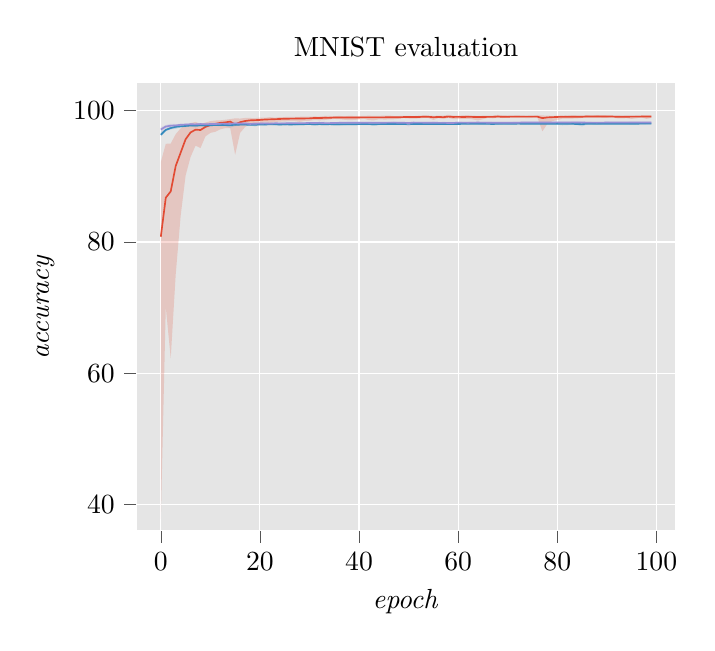
\begin{tikzpicture}

\definecolor{color0}{rgb}{0.886274509803922,0.290196078431373,0.2}
\definecolor{color1}{rgb}{0.203921568627451,0.541176470588235,0.741176470588235}
\definecolor{color2}{rgb}{0.596078431372549,0.556862745098039,0.835294117647059}

\begin{axis}[
axis background/.style={fill=white!89.8039215686275!black},
axis line style={white},
legend cell align={left},
legend style={fill opacity=0.8, draw opacity=1, text opacity=1, at={(0.03,0.03)}, anchor=south west, draw=white!80!black, fill=white!89.8039215686275!black},
log basis y={10},
tick align=outside,
tick pos=left,
title={MNIST evaluation},
x grid style={white},
xlabel={\textit{epoch}},
xmajorgrids,
xmin=-4.95, xmax=103.95,
xtick style={color=white!33.3333333333333!black},
y grid style={white},
ylabel={\textit{accuracy}},
ymajorgrids,
ymin=36.0171940474293, ymax=104.289020392695,
%ymode=log,
ytick style={color=white!33.3333333333333!black}
]
\path [fill=color0, fill opacity=0.2, very thin]
(axis cs:0,92.1575)
--(axis cs:0,37.8005)
--(axis cs:1,70.0821)
--(axis cs:2,62.3297)
--(axis cs:3,75.02)
--(axis cs:4,83.9744)
--(axis cs:5,90.1242)
--(axis cs:6,92.9387)
--(axis cs:7,94.6715)
--(axis cs:8,94.3109)
--(axis cs:9,96.0837)
--(axis cs:10,96.6146)
--(axis cs:11,96.7849)
--(axis cs:12,97.1554)
--(axis cs:13,97.3458)
--(axis cs:14,97.3558)
--(axis cs:15,93.2893)
--(axis cs:16,96.6146)
--(axis cs:17,97.516)
--(axis cs:18,97.9367)
--(axis cs:19,98.0268)
--(axis cs:20,98.0769)
--(axis cs:21,98.2071)
--(axis cs:22,98.127)
--(axis cs:23,98.2672)
--(axis cs:24,98.3373)
--(axis cs:25,98.3774)
--(axis cs:26,98.4175)
--(axis cs:27,98.3974)
--(axis cs:28,98.2973)
--(axis cs:29,98.4275)
--(axis cs:30,98.4575)
--(axis cs:31,98.5677)
--(axis cs:32,98.5276)
--(axis cs:33,98.5677)
--(axis cs:34,98.6679)
--(axis cs:35,98.738)
--(axis cs:36,98.7079)
--(axis cs:37,98.6178)
--(axis cs:38,98.5477)
--(axis cs:39,98.5877)
--(axis cs:40,98.6478)
--(axis cs:41,98.778)
--(axis cs:42,98.5477)
--(axis cs:43,98.5276)
--(axis cs:44,98.6879)
--(axis cs:45,98.6478)
--(axis cs:46,98.6579)
--(axis cs:47,98.6879)
--(axis cs:48,98.768)
--(axis cs:49,98.8582)
--(axis cs:50,98.8081)
--(axis cs:51,98.768)
--(axis cs:52,98.8181)
--(axis cs:53,98.8982)
--(axis cs:54,98.8882)
--(axis cs:55,98.5777)
--(axis cs:56,98.8682)
--(axis cs:57,98.728)
--(axis cs:58,98.9083)
--(axis cs:59,98.7179)
--(axis cs:60,98.728)
--(axis cs:61,98.738)
--(axis cs:62,98.768)
--(axis cs:63,98.6679)
--(axis cs:64,98.5076)
--(axis cs:65,98.7079)
--(axis cs:66,98.8982)
--(axis cs:67,98.8381)
--(axis cs:68,98.9583)
--(axis cs:69,98.8782)
--(axis cs:70,98.9583)
--(axis cs:71,98.8882)
--(axis cs:72,98.9183)
--(axis cs:73,98.9183)
--(axis cs:74,98.8482)
--(axis cs:75,98.9183)
--(axis cs:76,98.9583)
--(axis cs:77,96.845)
--(axis cs:78,97.9768)
--(axis cs:79,98.4175)
--(axis cs:80,98.5677)
--(axis cs:81,98.778)
--(axis cs:82,98.778)
--(axis cs:83,98.7981)
--(axis cs:84,98.8281)
--(axis cs:85,98.8982)
--(axis cs:86,98.9283)
--(axis cs:87,98.9483)
--(axis cs:88,98.9383)
--(axis cs:89,98.9183)
--(axis cs:90,98.9083)
--(axis cs:91,99.0184)
--(axis cs:92,98.8482)
--(axis cs:93,98.8181)
--(axis cs:94,98.8582)
--(axis cs:95,98.748)
--(axis cs:96,98.8482)
--(axis cs:97,98.9683)
--(axis cs:98,98.748)
--(axis cs:99,98.8982)
--(axis cs:99,99.2488)
--(axis cs:99,99.2488)
--(axis cs:98,99.2488)
--(axis cs:97,99.2688)
--(axis cs:96,99.2688)
--(axis cs:95,99.2488)
--(axis cs:94,99.2388)
--(axis cs:93,99.2087)
--(axis cs:92,99.2588)
--(axis cs:91,99.2488)
--(axis cs:90,99.2588)
--(axis cs:89,99.2889)
--(axis cs:88,99.3089)
--(axis cs:87,99.2188)
--(axis cs:86,99.3089)
--(axis cs:85,99.2288)
--(axis cs:84,99.2588)
--(axis cs:83,99.2788)
--(axis cs:82,99.2087)
--(axis cs:81,99.2788)
--(axis cs:80,99.2388)
--(axis cs:79,99.1987)
--(axis cs:78,99.2488)
--(axis cs:77,99.2688)
--(axis cs:76,99.2688)
--(axis cs:75,99.2588)
--(axis cs:74,99.2188)
--(axis cs:73,99.2288)
--(axis cs:72,99.2889)
--(axis cs:71,99.2488)
--(axis cs:70,99.2188)
--(axis cs:69,99.2388)
--(axis cs:68,99.349)
--(axis cs:67,99.2588)
--(axis cs:66,99.2288)
--(axis cs:65,99.2288)
--(axis cs:64,99.2087)
--(axis cs:63,99.2388)
--(axis cs:62,99.3189)
--(axis cs:61,99.2889)
--(axis cs:60,99.2188)
--(axis cs:59,99.2488)
--(axis cs:58,99.369)
--(axis cs:57,99.2288)
--(axis cs:56,99.2288)
--(axis cs:55,99.2188)
--(axis cs:54,99.2588)
--(axis cs:53,99.2688)
--(axis cs:52,99.2288)
--(axis cs:51,99.1687)
--(axis cs:50,99.1987)
--(axis cs:49,99.2188)
--(axis cs:48,99.1787)
--(axis cs:47,99.1787)
--(axis cs:46,99.2588)
--(axis cs:45,99.2388)
--(axis cs:44,99.2087)
--(axis cs:43,99.1887)
--(axis cs:42,99.2388)
--(axis cs:41,99.1987)
--(axis cs:40,99.1787)
--(axis cs:39,99.1787)
--(axis cs:38,99.2087)
--(axis cs:37,99.1186)
--(axis cs:36,99.2087)
--(axis cs:35,99.1286)
--(axis cs:34,99.1987)
--(axis cs:33,99.1987)
--(axis cs:32,99.0986)
--(axis cs:31,99.1186)
--(axis cs:30,99.0785)
--(axis cs:29,99.1086)
--(axis cs:28,99.0685)
--(axis cs:27,99.0385)
--(axis cs:26,99.0685)
--(axis cs:25,99.0284)
--(axis cs:24,99.0184)
--(axis cs:23,98.9283)
--(axis cs:22,99.0184)
--(axis cs:21,98.9183)
--(axis cs:20,98.9483)
--(axis cs:19,98.8582)
--(axis cs:18,98.8882)
--(axis cs:17,98.8882)
--(axis cs:16,98.7981)
--(axis cs:15,98.8281)
--(axis cs:14,98.7179)
--(axis cs:13,98.6178)
--(axis cs:12,98.5276)
--(axis cs:11,98.4976)
--(axis cs:10,98.4075)
--(axis cs:9,98.1771)
--(axis cs:8,98.0068)
--(axis cs:7,98.2772)
--(axis cs:6,98.117)
--(axis cs:5,97.7063)
--(axis cs:4,97.3057)
--(axis cs:3,96.4143)
--(axis cs:2,94.992)
--(axis cs:1,94.9519)
--(axis cs:0,92.1575)
--cycle;

\path [fill=color1, fill opacity=0.2, very thin]
(axis cs:0,96.7267)
--(axis cs:0,96.1036)
--(axis cs:1,96.875)
--(axis cs:2,97.1519)
--(axis cs:3,97.231)
--(axis cs:4,97.4684)
--(axis cs:5,97.4881)
--(axis cs:6,97.6068)
--(axis cs:7,97.4585)
--(axis cs:8,97.6266)
--(axis cs:9,97.4684)
--(axis cs:10,97.6365)
--(axis cs:11,97.7057)
--(axis cs:12,97.6266)
--(axis cs:13,97.6365)
--(axis cs:14,97.4288)
--(axis cs:15,97.6464)
--(axis cs:16,97.7156)
--(axis cs:17,97.7354)
--(axis cs:18,97.7453)
--(axis cs:19,97.5969)
--(axis cs:20,97.8046)
--(axis cs:21,97.7551)
--(axis cs:22,97.8343)
--(axis cs:23,97.7848)
--(axis cs:24,97.7354)
--(axis cs:25,97.765)
--(axis cs:26,97.7947)
--(axis cs:27,97.7255)
--(axis cs:28,97.7947)
--(axis cs:29,97.7749)
--(axis cs:30,97.8738)
--(axis cs:31,97.7156)
--(axis cs:32,97.7947)
--(axis cs:33,97.8046)
--(axis cs:34,97.8046)
--(axis cs:35,97.7255)
--(axis cs:36,97.7255)
--(axis cs:37,97.8046)
--(axis cs:38,97.8343)
--(axis cs:39,97.7848)
--(axis cs:40,97.8046)
--(axis cs:41,97.8145)
--(axis cs:42,97.8046)
--(axis cs:43,97.7057)
--(axis cs:44,97.8145)
--(axis cs:45,97.8441)
--(axis cs:46,97.854)
--(axis cs:47,97.8244)
--(axis cs:48,97.8244)
--(axis cs:49,97.854)
--(axis cs:50,97.8936)
--(axis cs:51,97.8343)
--(axis cs:52,97.8837)
--(axis cs:53,97.8343)
--(axis cs:54,97.854)
--(axis cs:55,97.9035)
--(axis cs:56,97.8738)
--(axis cs:57,97.8738)
--(axis cs:58,97.8441)
--(axis cs:59,97.8738)
--(axis cs:60,97.8936)
--(axis cs:61,97.9035)
--(axis cs:62,97.8837)
--(axis cs:63,97.9035)
--(axis cs:64,97.8936)
--(axis cs:65,97.8738)
--(axis cs:66,97.854)
--(axis cs:67,97.854)
--(axis cs:68,97.8441)
--(axis cs:69,97.8936)
--(axis cs:70,97.9035)
--(axis cs:71,97.8837)
--(axis cs:72,97.8936)
--(axis cs:73,97.8738)
--(axis cs:74,97.8936)
--(axis cs:75,97.8639)
--(axis cs:76,97.8837)
--(axis cs:77,97.8936)
--(axis cs:78,97.8837)
--(axis cs:79,97.854)
--(axis cs:80,97.8738)
--(axis cs:81,97.7749)
--(axis cs:82,97.7947)
--(axis cs:83,97.8837)
--(axis cs:84,97.8046)
--(axis cs:85,97.6068)
--(axis cs:86,97.9035)
--(axis cs:87,97.8936)
--(axis cs:88,97.8738)
--(axis cs:89,97.8936)
--(axis cs:90,97.9035)
--(axis cs:91,97.9233)
--(axis cs:92,97.8936)
--(axis cs:93,97.8936)
--(axis cs:94,97.9035)
--(axis cs:95,97.8837)
--(axis cs:96,97.8936)
--(axis cs:97,97.8837)
--(axis cs:98,97.8936)
--(axis cs:99,97.9233)
--(axis cs:99,98.1606)
--(axis cs:99,98.1606)
--(axis cs:98,98.1309)
--(axis cs:97,98.1309)
--(axis cs:96,98.1903)
--(axis cs:95,98.1903)
--(axis cs:94,98.1705)
--(axis cs:93,98.121)
--(axis cs:92,98.1804)
--(axis cs:91,98.121)
--(axis cs:90,98.1705)
--(axis cs:89,98.1606)
--(axis cs:88,98.1507)
--(axis cs:87,98.1112)
--(axis cs:86,98.1309)
--(axis cs:85,98.1112)
--(axis cs:84,98.1408)
--(axis cs:83,98.1804)
--(axis cs:82,98.1606)
--(axis cs:81,98.1606)
--(axis cs:80,98.1112)
--(axis cs:79,98.0914)
--(axis cs:78,98.1507)
--(axis cs:77,98.1705)
--(axis cs:76,98.1507)
--(axis cs:75,98.1309)
--(axis cs:74,98.1309)
--(axis cs:73,98.1903)
--(axis cs:72,98.1804)
--(axis cs:71,98.1606)
--(axis cs:70,98.121)
--(axis cs:69,98.1112)
--(axis cs:68,98.1507)
--(axis cs:67,98.0716)
--(axis cs:66,98.0914)
--(axis cs:65,98.0815)
--(axis cs:64,98.1112)
--(axis cs:63,98.0914)
--(axis cs:62,98.0815)
--(axis cs:61,98.0815)
--(axis cs:60,98.121)
--(axis cs:59,98.0815)
--(axis cs:58,98.0716)
--(axis cs:57,98.121)
--(axis cs:56,98.1507)
--(axis cs:55,98.0815)
--(axis cs:54,98.1309)
--(axis cs:53,98.1013)
--(axis cs:52,98.0716)
--(axis cs:51,98.0419)
--(axis cs:50,98.0914)
--(axis cs:49,98.1013)
--(axis cs:48,98.0914)
--(axis cs:47,98.0716)
--(axis cs:46,98.1013)
--(axis cs:45,98.1408)
--(axis cs:44,98.1013)
--(axis cs:43,98.0419)
--(axis cs:42,98.0716)
--(axis cs:41,98.0716)
--(axis cs:40,98.032)
--(axis cs:39,98.0617)
--(axis cs:38,98.0221)
--(axis cs:37,98.0024)
--(axis cs:36,98.0024)
--(axis cs:35,98.0024)
--(axis cs:34,98.1112)
--(axis cs:33,97.9925)
--(axis cs:32,98.0518)
--(axis cs:31,98.0221)
--(axis cs:30,98.1309)
--(axis cs:29,98.0419)
--(axis cs:28,98.0221)
--(axis cs:27,98.0716)
--(axis cs:26,98.0123)
--(axis cs:25,98.121)
--(axis cs:24,98.0419)
--(axis cs:23,98.0815)
--(axis cs:22,98.121)
--(axis cs:21,98.0716)
--(axis cs:20,98.0716)
--(axis cs:19,98.0914)
--(axis cs:18,98.0518)
--(axis cs:17,98.0518)
--(axis cs:16,98.0617)
--(axis cs:15,98.0123)
--(axis cs:14,97.9332)
--(axis cs:13,97.9529)
--(axis cs:12,97.9826)
--(axis cs:11,97.9727)
--(axis cs:10,98.032)
--(axis cs:9,97.943)
--(axis cs:8,97.854)
--(axis cs:7,97.8936)
--(axis cs:6,97.8738)
--(axis cs:5,97.8343)
--(axis cs:4,97.8046)
--(axis cs:3,97.7453)
--(axis cs:2,97.5672)
--(axis cs:1,97.2211)
--(axis cs:0,96.7267)
--cycle;

\path [fill=color2, fill opacity=0.2, very thin]
(axis cs:0,97.498022)
--(axis cs:0,96.696994)
--(axis cs:1,97.250791)
--(axis cs:2,97.428797)
--(axis cs:3,97.596915)
--(axis cs:4,97.685918)
--(axis cs:5,97.78481)
--(axis cs:6,97.65625)
--(axis cs:7,97.547468)
--(axis cs:8,97.676028)
--(axis cs:9,97.774921)
--(axis cs:10,97.755142)
--(axis cs:11,97.804589)
--(axis cs:12,97.903481)
--(axis cs:13,97.903481)
--(axis cs:14,97.873813)
--(axis cs:15,97.952927)
--(axis cs:16,97.873813)
--(axis cs:17,97.863924)
--(axis cs:18,97.745253)
--(axis cs:19,97.78481)
--(axis cs:20,97.78481)
--(axis cs:21,97.883703)
--(axis cs:22,97.854035)
--(axis cs:23,97.923259)
--(axis cs:24,97.883703)
--(axis cs:25,97.715585)
--(axis cs:26,97.834256)
--(axis cs:27,97.903481)
--(axis cs:28,97.933149)
--(axis cs:29,97.992484)
--(axis cs:30,98.04193)
--(axis cs:31,97.962816)
--(axis cs:32,97.982595)
--(axis cs:33,97.91337)
--(axis cs:34,97.883703)
--(axis cs:35,98.002373)
--(axis cs:36,98.022152)
--(axis cs:37,98.05182)
--(axis cs:38,97.972706)
--(axis cs:39,98.002373)
--(axis cs:40,97.933149)
--(axis cs:41,97.923259)
--(axis cs:42,98.022152)
--(axis cs:43,98.032041)
--(axis cs:44,98.061709)
--(axis cs:45,98.081487)
--(axis cs:46,98.012263)
--(axis cs:47,98.061709)
--(axis cs:48,98.081487)
--(axis cs:49,97.923259)
--(axis cs:50,97.606804)
--(axis cs:51,98.071598)
--(axis cs:52,98.111155)
--(axis cs:53,97.962816)
--(axis cs:54,98.022152)
--(axis cs:55,97.962816)
--(axis cs:56,97.943038)
--(axis cs:57,98.012263)
--(axis cs:58,98.002373)
--(axis cs:59,97.844146)
--(axis cs:60,98.04193)
--(axis cs:61,98.012263)
--(axis cs:62,97.982595)
--(axis cs:63,98.002373)
--(axis cs:64,98.022152)
--(axis cs:65,97.903481)
--(axis cs:66,97.992484)
--(axis cs:67,98.071598)
--(axis cs:68,98.04193)
--(axis cs:69,98.061709)
--(axis cs:70,97.903481)
--(axis cs:71,97.972706)
--(axis cs:72,97.933149)
--(axis cs:73,98.061709)
--(axis cs:74,98.05182)
--(axis cs:75,98.002373)
--(axis cs:76,97.982595)
--(axis cs:77,98.05182)
--(axis cs:78,98.012263)
--(axis cs:79,98.032041)
--(axis cs:80,98.071598)
--(axis cs:81,98.081487)
--(axis cs:82,97.854035)
--(axis cs:83,98.05182)
--(axis cs:84,97.91337)
--(axis cs:85,98.012263)
--(axis cs:86,97.962816)
--(axis cs:87,98.002373)
--(axis cs:88,97.903481)
--(axis cs:89,98.091377)
--(axis cs:90,98.101266)
--(axis cs:91,98.111155)
--(axis cs:92,98.04193)
--(axis cs:93,98.140823)
--(axis cs:94,98.05182)
--(axis cs:95,98.012263)
--(axis cs:96,98.032041)
--(axis cs:97,98.081487)
--(axis cs:98,97.933149)
--(axis cs:99,98.071598)
--(axis cs:99,98.318829)
--(axis cs:99,98.318829)
--(axis cs:98,98.328718)
--(axis cs:97,98.30894)
--(axis cs:96,98.328718)
--(axis cs:95,98.328718)
--(axis cs:94,98.299051)
--(axis cs:93,98.299051)
--(axis cs:92,98.299051)
--(axis cs:91,98.299051)
--(axis cs:90,98.318829)
--(axis cs:89,98.299051)
--(axis cs:88,98.30894)
--(axis cs:87,98.30894)
--(axis cs:86,98.328718)
--(axis cs:85,98.299051)
--(axis cs:84,98.368275)
--(axis cs:83,98.358386)
--(axis cs:82,98.318829)
--(axis cs:81,98.338608)
--(axis cs:80,98.318829)
--(axis cs:79,98.299051)
--(axis cs:78,98.348497)
--(axis cs:77,98.328718)
--(axis cs:76,98.328718)
--(axis cs:75,98.318829)
--(axis cs:74,98.338608)
--(axis cs:73,98.328718)
--(axis cs:72,98.348497)
--(axis cs:71,98.30894)
--(axis cs:70,98.299051)
--(axis cs:69,98.30894)
--(axis cs:68,98.279272)
--(axis cs:67,98.30894)
--(axis cs:66,98.318829)
--(axis cs:65,98.348497)
--(axis cs:64,98.328718)
--(axis cs:63,98.328718)
--(axis cs:62,98.30894)
--(axis cs:61,98.30894)
--(axis cs:60,98.318829)
--(axis cs:59,98.299051)
--(axis cs:58,98.299051)
--(axis cs:57,98.318829)
--(axis cs:56,98.289161)
--(axis cs:55,98.318829)
--(axis cs:54,98.289161)
--(axis cs:53,98.279272)
--(axis cs:52,98.30894)
--(axis cs:51,98.289161)
--(axis cs:50,98.269383)
--(axis cs:49,98.30894)
--(axis cs:48,98.269383)
--(axis cs:47,98.358386)
--(axis cs:46,98.279272)
--(axis cs:45,98.229826)
--(axis cs:44,98.269383)
--(axis cs:43,98.259494)
--(axis cs:42,98.289161)
--(axis cs:41,98.269383)
--(axis cs:40,98.328718)
--(axis cs:39,98.279272)
--(axis cs:38,98.30894)
--(axis cs:37,98.239715)
--(axis cs:36,98.299051)
--(axis cs:35,98.229826)
--(axis cs:34,98.229826)
--(axis cs:33,98.318829)
--(axis cs:32,98.249604)
--(axis cs:31,98.210047)
--(axis cs:30,98.239715)
--(axis cs:29,98.170491)
--(axis cs:28,98.160601)
--(axis cs:27,98.18038)
--(axis cs:26,98.269383)
--(axis cs:25,98.348497)
--(axis cs:24,98.190269)
--(axis cs:23,98.190269)
--(axis cs:22,98.229826)
--(axis cs:21,98.210047)
--(axis cs:20,98.229826)
--(axis cs:19,98.229826)
--(axis cs:18,98.111155)
--(axis cs:17,98.239715)
--(axis cs:16,98.200158)
--(axis cs:15,98.30894)
--(axis cs:14,98.140823)
--(axis cs:13,98.190269)
--(axis cs:12,98.160601)
--(axis cs:11,98.081487)
--(axis cs:10,98.130934)
--(axis cs:9,98.121044)
--(axis cs:8,98.111155)
--(axis cs:7,98.05182)
--(axis cs:6,98.101266)
--(axis cs:5,98.002373)
--(axis cs:4,97.972706)
--(axis cs:3,97.962816)
--(axis cs:2,98.002373)
--(axis cs:1,97.804589)
--(axis cs:0,97.498022)
--cycle;

\addplot [semithick, color0]
table {%
0 80.7982864379883
1 86.7437896728516
2 87.709342956543
3 91.5675201416016
5 95.64404296875
6 96.6827087402344
7 97.1043701171875
8 97.0522766113281
9 97.5240325927734
10 97.8074798583984
11 97.9937896728516
12 98.1440200805664
13 98.2091293334961
14 98.3343200683594
15 97.8976440429688
16 98.2442092895508
17 98.4244842529297
18 98.5246276855469
20 98.5877456665039
21 98.6498413085938
23 98.6999206542969
25 98.7680282592773
30 98.828125
31 98.8902359008789
32 98.8701782226562
33 98.9082412719727
34 98.9072570800781
35 98.9563293457031
48 98.9913787841797
49 99.0254592895508
52 99.0304870605469
53 99.0765151977539
54 99.0655059814453
55 99.0024108886719
56 99.0444869995117
57 99.0094223022461
58 99.0935668945312
59 99.0414657592773
60 99.0615081787109
61 99.032470703125
62 99.0574798583984
65 99.0224380493164
66 99.0565032958984
67 99.0494842529297
68 99.1015625
69 99.0634918212891
71 99.0925598144531
76 99.0855484008789
77 98.8631820678711
78 98.9713821411133
80 99.0444869995117
83 99.0765151977539
85 99.0755386352539
86 99.1135940551758
88 99.0995559692383
90 99.110595703125
91 99.1085815429688
92 99.0685195922852
99 99.1105728149414
};
%\addlegendentry{cudnn}
\addplot [semithick, color1]
table {%
0 96.3271408081055
1 97.0688171386719
2 97.3486938476562
3 97.5425338745117
6 97.7353363037109
7 97.7235107421875
8 97.7779006958008
9 97.7432556152344
11 97.8065643310547
12 97.7956695556641
13 97.8243637084961
14 97.791748046875
15 97.8530502319336
17 97.8817367553711
18 97.8293075561523
19 97.8382263183594
20 97.9044723510742
21 97.8738098144531
22 97.940055847168
23 97.9351425170898
24 97.880744934082
25 97.92919921875
26 97.8945846557617
30 97.958854675293
31 97.9064331054688
32 97.9529113769531
33 97.9133911132812
34 97.9459991455078
36 97.9173202514648
38 97.9341430664062
40 97.9440078735352
41 97.978645324707
43 97.9262161254883
45 97.9727020263672
49 97.9608688354492
50 97.9934616088867
51 97.959846496582
66 97.9924697875977
67 97.9677810668945
68 98.0033645629883
70 97.9895095825195
72 98.0201797485352
84 97.978645324707
85 97.9469985961914
86 98.0092849731445
88 97.9994049072266
90 98.0142288208008
99 98.0201797485352
};
%\addlegendentry{libtorch}
\addplot [semithick, color2]
table {%
0 97.1321182250977
1 97.5870132446289
2 97.7126159667969
3 97.7462310791016
4 97.8530502319336
6 97.9252471923828
7 97.9133682250977
8 97.9618377685547
9 97.9301910400391
10 97.9647979736328
11 97.9578552246094
12 98.0261001586914
14 98.0033645629883
15 98.0676498413086
16 98.0359954833984
17 98.0587387084961
18 97.9756622314453
20 98.0379638671875
21 98.0616989135742
22 98.0231399536133
23 98.0735702514648
25 98.0616989135742
26 98.0992813110352
29 98.095329284668
30 98.1408157348633
31 98.1190490722656
32 98.1497344970703
33 98.1062088012695
34 98.1042404174805
36 98.1467666625977
37 98.1605911254883
39 98.1487350463867
43 98.1605911254883
47 98.1764373779297
49 98.1556625366211
50 98.1141204833984
51 98.1853256225586
59 98.1220397949219
60 98.1843338012695
62 98.1685104370117
64 98.1872940063477
66 98.1675186157227
71 98.1615905761719
72 98.1536636352539
73 98.2021484375
78 98.1902618408203
80 98.2120361328125
82 98.1843338012695
83 98.2140045166016
85 98.1882934570312
88 98.1705093383789
90 98.1892929077148
99 98.2021484375
};
%\addlegendentry{pytorch}
\end{axis}

\end{tikzpicture}

    \end{figure}


    \begin{figure}
        % This file was created by tikzplotlib v0.9.5.
\begin{tikzpicture}





\begin{axis}[
axis background/.style={fill=white!89.8039215686275!black},
axis line style={white},
legend cell align={left},
legend style={fill opacity=0.8, draw opacity=1, text opacity=1, at={(0.97,0.03)}, anchor=south east, draw=white!80!black, fill=white!89.8039215686275!black},
log basis y={10},
tick align=outside,
tick pos=left,
title={CIFAR10 evaluation},
x grid style={white},
xlabel={epoch},
xmajorgrids,
xmin=-4.95, xmax=103.95,
xtick style={color=white!33.3333333333333!black},
y grid style={white},
ymajorgrids,
ymin=15.7517645561491, ymax=80.8079673084566,
%ymode=log,
ytick style={color=white!33.3333333333333!black}
]
\path [fill=cudnn, fill opacity=0.2, very thin]
(axis cs:0,22.2756)
--(axis cs:0,16.9671)
--(axis cs:1,22.0553)
--(axis cs:2,23.8281)
--(axis cs:3,24.1787)
--(axis cs:4,24.9499)
--(axis cs:5,24.97)
--(axis cs:6,25.9115)
--(axis cs:7,27.2336)
--(axis cs:8,28.145)
--(axis cs:9,29.2167)
--(axis cs:10,30.6791)
--(axis cs:11,34.2949)
--(axis cs:12,36.5986)
--(axis cs:13,38.8321)
--(axis cs:14,32.0112)
--(axis cs:15,36.5785)
--(axis cs:16,38.5116)
--(axis cs:17,40.1042)
--(axis cs:18,42.8786)
--(axis cs:19,44.5413)
--(axis cs:20,46.1038)
--(axis cs:21,47.5561)
--(axis cs:22,48.9383)
--(axis cs:23,49.5893)
--(axis cs:24,51.1619)
--(axis cs:25,52.3638)
--(axis cs:26,52.9748)
--(axis cs:27,53.9463)
--(axis cs:28,54.4872)
--(axis cs:29,54.8177)
--(axis cs:30,55.599)
--(axis cs:31,56.3001)
--(axis cs:32,57.0112)
--(axis cs:33,57.7524)
--(axis cs:34,57.8826)
--(axis cs:35,58.7841)
--(axis cs:36,59.3049)
--(axis cs:37,59.7456)
--(axis cs:38,60.2965)
--(axis cs:39,60.7272)
--(axis cs:40,61.4183)
--(axis cs:41,61.7388)
--(axis cs:42,62.1294)
--(axis cs:43,62.6703)
--(axis cs:44,62.9307)
--(axis cs:45,63.4115)
--(axis cs:46,63.5517)
--(axis cs:47,63.6318)
--(axis cs:48,63.9223)
--(axis cs:49,64.0325)
--(axis cs:50,64.6735)
--(axis cs:51,64.5633)
--(axis cs:52,65.1542)
--(axis cs:53,65.2244)
--(axis cs:54,65.5349)
--(axis cs:55,65.5749)
--(axis cs:56,65.5449)
--(axis cs:57,66.1258)
--(axis cs:58,66.2059)
--(axis cs:59,66.5966)
--(axis cs:60,66.7368)
--(axis cs:61,66.897)
--(axis cs:62,67.0673)
--(axis cs:63,67.0873)
--(axis cs:64,67.528)
--(axis cs:65,67.6683)
--(axis cs:66,67.5982)
--(axis cs:67,68.109)
--(axis cs:68,68.2993)
--(axis cs:69,68.3994)
--(axis cs:70,68.4595)
--(axis cs:71,68.4395)
--(axis cs:72,68.5196)
--(axis cs:73,68.77)
--(axis cs:74,68.5296)
--(axis cs:75,68.9603)
--(axis cs:76,68.9002)
--(axis cs:77,68.5397)
--(axis cs:78,69.0605)
--(axis cs:79,69.4111)
--(axis cs:80,69.0204)
--(axis cs:81,69.1506)
--(axis cs:82,69.2608)
--(axis cs:83,69.6014)
--(axis cs:84,69.7917)
--(axis cs:85,69.6715)
--(axis cs:86,69.7917)
--(axis cs:87,69.8017)
--(axis cs:88,69.9119)
--(axis cs:89,69.6314)
--(axis cs:90,69.8718)
--(axis cs:91,70.0621)
--(axis cs:92,69.6014)
--(axis cs:93,70.4527)
--(axis cs:94,70.3325)
--(axis cs:95,70.2724)
--(axis cs:96,70.7532)
--(axis cs:97,70.3025)
--(axis cs:98,70.7031)
--(axis cs:99,70.8734)
--(axis cs:99,72.3958)
--(axis cs:99,72.3958)
--(axis cs:98,72.486)
--(axis cs:97,72.7764)
--(axis cs:96,72.4459)
--(axis cs:95,72.496)
--(axis cs:94,72.3357)
--(axis cs:93,72.2756)
--(axis cs:92,72.4159)
--(axis cs:91,72.5561)
--(axis cs:90,72.2055)
--(axis cs:89,72.2556)
--(axis cs:88,72.3458)
--(axis cs:87,72.4159)
--(axis cs:86,72.6763)
--(axis cs:85,72.496)
--(axis cs:84,72.4058)
--(axis cs:83,72.6262)
--(axis cs:82,72.3658)
--(axis cs:81,72.526)
--(axis cs:80,72.0753)
--(axis cs:79,72.4459)
--(axis cs:78,72.4559)
--(axis cs:77,72.2756)
--(axis cs:76,72.506)
--(axis cs:75,72.4559)
--(axis cs:74,72.4659)
--(axis cs:73,72.526)
--(axis cs:72,72.3658)
--(axis cs:71,72.2756)
--(axis cs:70,72.2155)
--(axis cs:69,72.0252)
--(axis cs:68,72.2456)
--(axis cs:67,71.845)
--(axis cs:66,71.7949)
--(axis cs:65,71.8049)
--(axis cs:64,71.6346)
--(axis cs:63,71.3842)
--(axis cs:62,71.7748)
--(axis cs:61,71.1739)
--(axis cs:60,71.5044)
--(axis cs:59,71.254)
--(axis cs:58,71.274)
--(axis cs:57,71.0938)
--(axis cs:56,71.0537)
--(axis cs:55,70.9635)
--(axis cs:54,70.9135)
--(axis cs:53,70.5028)
--(axis cs:52,70.4327)
--(axis cs:51,70.2524)
--(axis cs:50,70.3025)
--(axis cs:49,70.3926)
--(axis cs:48,70.1522)
--(axis cs:47,69.7516)
--(axis cs:46,69.9219)
--(axis cs:45,69.5513)
--(axis cs:44,69.3009)
--(axis cs:43,69.391)
--(axis cs:42,69.1907)
--(axis cs:41,69.0605)
--(axis cs:40,68.4195)
--(axis cs:39,68.3093)
--(axis cs:38,68.2492)
--(axis cs:37,67.6683)
--(axis cs:36,67.8486)
--(axis cs:35,67.4279)
--(axis cs:34,67.1474)
--(axis cs:33,66.6767)
--(axis cs:32,66.2159)
--(axis cs:31,65.8353)
--(axis cs:30,65.6951)
--(axis cs:29,65.7452)
--(axis cs:28,64.6935)
--(axis cs:27,64.8337)
--(axis cs:26,64.2628)
--(axis cs:25,63.6218)
--(axis cs:24,63.4816)
--(axis cs:23,62.3998)
--(axis cs:22,61.1378)
--(axis cs:21,60.1162)
--(axis cs:20,59.5753)
--(axis cs:19,60.607)
--(axis cs:18,60.1062)
--(axis cs:17,59.1046)
--(axis cs:16,58.2031)
--(axis cs:15,57.1915)
--(axis cs:14,55.9996)
--(axis cs:13,54.6474)
--(axis cs:12,53.5357)
--(axis cs:11,52.0333)
--(axis cs:10,50.1102)
--(axis cs:9,48.2071)
--(axis cs:8,47.0954)
--(axis cs:7,44.7416)
--(axis cs:6,42.2476)
--(axis cs:5,38.6819)
--(axis cs:4,37.0593)
--(axis cs:3,33.5737)
--(axis cs:2,31.5405)
--(axis cs:1,29.3269)
--(axis cs:0,22.2756)
--cycle;

\path [fill=libtorch, fill opacity=0.2, very thin]
(axis cs:0,45.7278)
--(axis cs:0,41.9205)
--(axis cs:1,47.765)
--(axis cs:2,51.0384)
--(axis cs:3,53.1349)
--(axis cs:4,53.6689)
--(axis cs:5,55.1028)
--(axis cs:6,57.051)
--(axis cs:7,57.6048)
--(axis cs:8,57.2884)
--(axis cs:9,57.3675)
--(axis cs:10,59.6519)
--(axis cs:11,58.3366)
--(axis cs:12,58.6926)
--(axis cs:13,57.7136)
--(axis cs:14,58.9498)
--(axis cs:15,60.6309)
--(axis cs:16,60.4331)
--(axis cs:17,60.3441)
--(axis cs:18,61.6297)
--(axis cs:19,61.3133)
--(axis cs:20,60.8386)
--(axis cs:21,61.9363)
--(axis cs:22,60.621)
--(axis cs:23,59.7805)
--(axis cs:24,62.2231)
--(axis cs:25,62.5198)
--(axis cs:26,61.5605)
--(axis cs:27,60.5815)
--(axis cs:28,61.6891)
--(axis cs:29,62.5791)
--(axis cs:30,62.5791)
--(axis cs:31,63.2812)
--(axis cs:32,63.301)
--(axis cs:33,63.1527)
--(axis cs:34,63.7757)
--(axis cs:35,62.8659)
--(axis cs:36,63.2615)
--(axis cs:37,63.0637)
--(axis cs:38,62.6385)
--(axis cs:39,63.4691)
--(axis cs:40,63.8153)
--(axis cs:41,63.8746)
--(axis cs:42,62.4308)
--(axis cs:43,63.4691)
--(axis cs:44,63.1428)
--(axis cs:45,63.8845)
--(axis cs:46,63.8647)
--(axis cs:47,63.8647)
--(axis cs:48,63.4395)
--(axis cs:49,64.468)
--(axis cs:50,63.5977)
--(axis cs:51,63.9735)
--(axis cs:52,64.3295)
--(axis cs:53,63.3604)
--(axis cs:54,63.924)
--(axis cs:55,63.5087)
--(axis cs:56,63.7065)
--(axis cs:57,64.4877)
--(axis cs:58,64.1021)
--(axis cs:59,64.1515)
--(axis cs:60,63.9735)
--(axis cs:61,64.4284)
--(axis cs:62,64.5372)
--(axis cs:63,64.9723)
--(axis cs:64,64.4877)
--(axis cs:65,64.4185)
--(axis cs:66,63.8153)
--(axis cs:67,63.8845)
--(axis cs:68,64.3691)
--(axis cs:69,63.8647)
--(axis cs:70,64.0922)
--(axis cs:71,64.0427)
--(axis cs:72,64.557)
--(axis cs:73,63.5186)
--(axis cs:74,64.6064)
--(axis cs:75,64.5668)
--(axis cs:76,64.1218)
--(axis cs:77,64.3888)
--(axis cs:78,63.9537)
--(axis cs:79,64.6756)
--(axis cs:80,64.5174)
--(axis cs:81,64.5767)
--(axis cs:82,63.6966)
--(axis cs:83,64.6855)
--(axis cs:84,64.824)
--(axis cs:85,64.9822)
--(axis cs:86,64.7251)
--(axis cs:87,64.4779)
--(axis cs:88,64.9921)
--(axis cs:89,65.269)
--(axis cs:90,64.6954)
--(axis cs:91,65.091)
--(axis cs:92,65.3283)
--(axis cs:93,65.2591)
--(axis cs:94,64.5273)
--(axis cs:95,64.6657)
--(axis cs:96,65.002)
--(axis cs:97,64.8833)
--(axis cs:98,65.1108)
--(axis cs:99,65.2888)
--(axis cs:99,67.5336)
--(axis cs:99,67.5336)
--(axis cs:98,67.3358)
--(axis cs:97,67.0985)
--(axis cs:96,67.2567)
--(axis cs:95,67.2271)
--(axis cs:94,67.2666)
--(axis cs:93,67.3952)
--(axis cs:92,67.0392)
--(axis cs:91,66.9699)
--(axis cs:90,67.3062)
--(axis cs:89,67.5831)
--(axis cs:88,67.0293)
--(axis cs:87,67.4941)
--(axis cs:86,67.3457)
--(axis cs:85,67.2073)
--(axis cs:84,66.4854)
--(axis cs:83,66.8809)
--(axis cs:82,66.9304)
--(axis cs:81,66.6733)
--(axis cs:80,66.9106)
--(axis cs:79,66.7029)
--(axis cs:78,67.1084)
--(axis cs:77,67.2271)
--(axis cs:76,67.1974)
--(axis cs:75,67.3161)
--(axis cs:74,67.5732)
--(axis cs:73,67.6523)
--(axis cs:72,67.3358)
--(axis cs:71,67.3952)
--(axis cs:70,66.7524)
--(axis cs:69,66.8315)
--(axis cs:68,66.6832)
--(axis cs:67,66.8315)
--(axis cs:66,66.8414)
--(axis cs:65,66.9403)
--(axis cs:64,67.049)
--(axis cs:63,66.6535)
--(axis cs:62,66.9502)
--(axis cs:61,66.6832)
--(axis cs:60,66.3667)
--(axis cs:59,66.337)
--(axis cs:58,66.6832)
--(axis cs:57,66.2678)
--(axis cs:56,66.5546)
--(axis cs:55,66.6832)
--(axis cs:54,66.3766)
--(axis cs:53,66.8315)
--(axis cs:52,66.1096)
--(axis cs:51,66.2282)
--(axis cs:50,66.4557)
--(axis cs:49,67.0985)
--(axis cs:48,66.7326)
--(axis cs:47,66.6337)
--(axis cs:46,66.4755)
--(axis cs:45,66.0502)
--(axis cs:44,66.0206)
--(axis cs:43,66.3172)
--(axis cs:42,65.7832)
--(axis cs:41,66.4854)
--(axis cs:40,66.426)
--(axis cs:39,65.9019)
--(axis cs:38,66.0502)
--(axis cs:37,66.2381)
--(axis cs:36,65.4173)
--(axis cs:35,65.625)
--(axis cs:34,65.4371)
--(axis cs:33,65.625)
--(axis cs:32,65.3184)
--(axis cs:31,65.3778)
--(axis cs:30,65.1899)
--(axis cs:29,65.1305)
--(axis cs:28,64.8932)
--(axis cs:27,65.625)
--(axis cs:26,64.8042)
--(axis cs:25,64.6262)
--(axis cs:24,65.0218)
--(axis cs:23,64.9624)
--(axis cs:22,64.5866)
--(axis cs:21,64.1416)
--(axis cs:20,63.6669)
--(axis cs:19,64.0328)
--(axis cs:18,63.3703)
--(axis cs:17,64.2801)
--(axis cs:16,63.8449)
--(axis cs:15,62.9747)
--(axis cs:14,63.7362)
--(axis cs:13,62.0945)
--(axis cs:12,62.1934)
--(axis cs:11,62.7176)
--(axis cs:10,61.6693)
--(axis cs:9,61.5012)
--(axis cs:8,61.1254)
--(axis cs:7,59.8794)
--(axis cs:6,60.3639)
--(axis cs:5,59.9288)
--(axis cs:4,58.6432)
--(axis cs:3,57.6543)
--(axis cs:2,54.3809)
--(axis cs:1,52.0372)
--(axis cs:0,45.7278)
--cycle;

\path [fill=pytorch, fill opacity=0.2, very thin]
(axis cs:0,54.153481)
--(axis cs:0,49.129747)
--(axis cs:1,54.252373)
--(axis cs:2,53.065665)
--(axis cs:3,55.676424)
--(axis cs:4,61.115506)
--(axis cs:5,54.924842)
--(axis cs:6,61.382516)
--(axis cs:7,58.356408)
--(axis cs:8,64.576741)
--(axis cs:9,63.399921)
--(axis cs:10,60.116693)
--(axis cs:11,66.742484)
--(axis cs:12,62.717563)
--(axis cs:13,65.516218)
--(axis cs:14,66.900712)
--(axis cs:15,65.921677)
--(axis cs:16,66.129351)
--(axis cs:17,68.571994)
--(axis cs:18,64.566851)
--(axis cs:19,66.574367)
--(axis cs:20,68.819225)
--(axis cs:21,66.821598)
--(axis cs:22,68.255538)
--(axis cs:23,69.323576)
--(axis cs:24,69.195016)
--(axis cs:25,66.040348)
--(axis cs:26,68.918117)
--(axis cs:27,65.704114)
--(axis cs:28,68.710443)
--(axis cs:29,68.87856)
--(axis cs:30,69.649921)
--(axis cs:31,69.293908)
--(axis cs:32,69.768592)
--(axis cs:33,70.549842)
--(axis cs:34,69.877373)
--(axis cs:35,70.213608)
--(axis cs:36,70.015823)
--(axis cs:37,70.826741)
--(axis cs:38,70.480617)
--(axis cs:39,69.768592)
--(axis cs:40,69.412579)
--(axis cs:41,70.44106)
--(axis cs:42,71.400316)
--(axis cs:43,71.143196)
--(axis cs:44,70.460839)
--(axis cs:45,70.223497)
--(axis cs:46,70.352057)
--(axis cs:47,71.370649)
--(axis cs:48,70.994858)
--(axis cs:49,69.541139)
--(axis cs:50,70.866297)
--(axis cs:51,71.538766)
--(axis cs:52,71.212421)
--(axis cs:53,70.530063)
--(axis cs:54,71.696994)
--(axis cs:55,71.064082)
--(axis cs:56,71.192642)
--(axis cs:57,70.094937)
--(axis cs:58,71.380538)
--(axis cs:59,71.301424)
--(axis cs:60,71.934335)
--(axis cs:61,71.657437)
--(axis cs:62,68.453323)
--(axis cs:63,71.420095)
--(axis cs:64,72.082674)
--(axis cs:65,72.072785)
--(axis cs:66,71.914557)
--(axis cs:67,72.221123)
--(axis cs:68,72.349684)
--(axis cs:69,71.568434)
--(axis cs:70,70.658623)
--(axis cs:71,71.74644)
--(axis cs:72,70.154272)
--(axis cs:73,71.716772)
--(axis cs:74,71.954114)
--(axis cs:75,72.013449)
--(axis cs:76,71.677215)
--(axis cs:77,71.894778)
--(axis cs:78,71.973892)
--(axis cs:79,72.359573)
--(axis cs:80,70.035601)
--(axis cs:81,71.400316)
--(axis cs:82,72.102453)
--(axis cs:83,71.123418)
--(axis cs:84,72.39913)
--(axis cs:85,70.935522)
--(axis cs:86,72.676028)
--(axis cs:87,72.606804)
--(axis cs:88,72.478244)
--(axis cs:89,72.626582)
--(axis cs:90,72.478244)
--(axis cs:91,71.677215)
--(axis cs:92,72.290348)
--(axis cs:93,72.300237)
--(axis cs:94,72.082674)
--(axis cs:95,72.27057)
--(axis cs:96,72.409019)
--(axis cs:97,72.458465)
--(axis cs:98,71.706883)
--(axis cs:99,72.26068)
--(axis cs:99,74.278085)
--(axis cs:99,74.278085)
--(axis cs:98,73.684731)
--(axis cs:97,74.060522)
--(axis cs:96,73.83307)
--(axis cs:95,74.386867)
--(axis cs:94,75.019778)
--(axis cs:93,74.920886)
--(axis cs:92,74.950554)
--(axis cs:91,74.673655)
--(axis cs:90,74.258307)
--(axis cs:89,73.951741)
--(axis cs:88,73.486946)
--(axis cs:87,74.149525)
--(axis cs:86,73.862737)
--(axis cs:85,73.753956)
--(axis cs:84,73.882516)
--(axis cs:83,73.714399)
--(axis cs:82,73.981408)
--(axis cs:81,73.397943)
--(axis cs:80,74.109968)
--(axis cs:79,74.179193)
--(axis cs:78,73.506725)
--(axis cs:77,73.82318)
--(axis cs:76,73.724288)
--(axis cs:75,73.239715)
--(axis cs:74,73.516614)
--(axis cs:73,73.704509)
--(axis cs:72,73.813291)
--(axis cs:71,73.664953)
--(axis cs:70,73.842959)
--(axis cs:69,73.585839)
--(axis cs:68,73.773734)
--(axis cs:67,73.289161)
--(axis cs:66,73.575949)
--(axis cs:65,73.358386)
--(axis cs:64,73.160601)
--(axis cs:63,73.813291)
--(axis cs:62,73.575949)
--(axis cs:61,73.407832)
--(axis cs:60,73.299051)
--(axis cs:59,72.735364)
--(axis cs:58,72.91337)
--(axis cs:57,73.002373)
--(axis cs:56,72.933149)
--(axis cs:55,73.378165)
--(axis cs:54,73.338608)
--(axis cs:53,73.486946)
--(axis cs:52,73.150712)
--(axis cs:51,73.022152)
--(axis cs:50,72.844146)
--(axis cs:49,73.318829)
--(axis cs:48,72.982595)
--(axis cs:47,73.022152)
--(axis cs:46,72.883703)
--(axis cs:45,72.824367)
--(axis cs:44,72.685918)
--(axis cs:43,72.844146)
--(axis cs:42,73.338608)
--(axis cs:41,72.349684)
--(axis cs:40,72.616693)
--(axis cs:39,72.626582)
--(axis cs:38,72.369462)
--(axis cs:37,73.239715)
--(axis cs:36,72.52769)
--(axis cs:35,72.547468)
--(axis cs:34,72.033228)
--(axis cs:33,72.161788)
--(axis cs:32,71.924446)
--(axis cs:31,72.478244)
--(axis cs:30,72.201345)
--(axis cs:29,72.488133)
--(axis cs:28,72.142009)
--(axis cs:27,71.420095)
--(axis cs:26,71.311313)
--(axis cs:25,71.439873)
--(axis cs:24,71.795886)
--(axis cs:23,72.52769)
--(axis cs:22,71.281646)
--(axis cs:21,72.409019)
--(axis cs:20,71.044304)
--(axis cs:19,71.034415)
--(axis cs:18,71.687104)
--(axis cs:17,70.866297)
--(axis cs:16,70.450949)
--(axis cs:15,70.381725)
--(axis cs:14,70.727848)
--(axis cs:13,70.747627)
--(axis cs:12,69.857595)
--(axis cs:11,69.551028)
--(axis cs:10,68.502769)
--(axis cs:9,69.946598)
--(axis cs:8,70.352057)
--(axis cs:7,67.592959)
--(axis cs:6,67.622627)
--(axis cs:5,66.960047)
--(axis cs:4,65.990902)
--(axis cs:3,64.893196)
--(axis cs:2,63.815269)
--(axis cs:1,60.215585)
--(axis cs:0,54.153481)
--cycle;

\addplot [semithick, cudnn]
table {%
0 20.3896198272705
1 24.7235527038574
2 27.6973209381104
3 29.6133804321289
4 32.2686347961426
5 34.1556663513184
6 35.9986000061035
7 37.7153549194336
8 39.4130516052246
9 40.8022880554199
10 42.3437614440918
11 44.1957244873047
13 46.9310646057129
14 46.7427825927734
15 48.2922515869141
16 49.5753059387207
17 50.7982864379883
18 52.1123924255371
19 53.132022857666
20 53.4134674072266
21 54.6864967346191
22 55.8002662658691
24 57.4719657897949
26 58.7840576171875
27 59.3119049072266
28 59.9799652099609
30 60.8153076171875
31 61.360179901123
32 61.8129081726074
33 62.3918151855469
34 62.6311988830566
35 63.1410140991211
36 63.5236396789551
37 63.8120994567871
38 64.1576385498047
40 64.6895217895508
41 65.2303619384766
42 65.5038070678711
44 65.9635467529297
45 66.2730560302734
46 66.4983901977539
47 66.6316070556641
48 66.9350814819336
49 67.0803298950195
50 67.3437423706055
51 67.485969543457
52 67.7634201049805
53 67.8525772094727
54 67.9847717285156
55 68.3333206176758
57 68.5366668701172
60 69.184700012207
61 69.2127532958984
62 69.340934753418
63 69.3960418701172
64 69.6223831176758
65 69.7736358642578
66 69.8207244873047
68 70.2133483886719
69 70.2533874511719
70 70.3355331420898
71 70.4787521362305
72 70.5578842163086
73 70.5919418334961
74 70.5839157104492
77 70.6930999755859
78 70.8844375610352
79 70.8724136352539
80 70.7562103271484
81 71.0045700073242
82 71.1488418579102
84 71.265022277832
85 71.2139434814453
86 71.4463119506836
87 71.3992462158203
88 71.4373092651367
89 71.3601760864258
90 71.421272277832
91 71.3481521606445
92 71.377197265625
94 71.5594787597656
95 71.4132537841797
96 71.5885391235352
97 71.5755310058594
98 71.6977233886719
99 71.6085662841797
};
%\addlegendentry{cudnn}
\addplot [semithick, libtorch]
table {%
0 44.0516204833984
1 50.2492065429688
2 52.7126274108887
3 55.1443901062012
4 56.1491165161133
5 57.9034729003906
6 58.8113021850586
7 59.0387763977051
8 59.1574554443359
10 60.7456359863281
11 60.8089485168457
12 60.6892547607422
13 60.8831024169922
14 61.2964782714844
15 61.6297492980957
16 62.0361862182617
17 61.8235778808594
18 62.4376792907715
19 62.5979080200195
20 62.6107597351074
21 62.8916244506836
22 62.8382186889648
23 63.1714935302734
24 63.6026573181152
25 63.7124252319336
26 63.4157447814941
27 63.7885627746582
28 63.7302131652832
29 63.8558158874512
31 64.4442367553711
32 64.3858871459961
33 64.4986190795898
34 64.7023239135742
35 64.384880065918
36 64.4887237548828
37 64.8882522583008
38 64.6390609741211
39 64.7013626098633
40 65.1067886352539
41 65.1928405761719
42 65.018798828125
43 65.1433868408203
44 64.9199142456055
45 64.8565979003906
46 65.1968154907227
47 65.1730575561523
48 65.4549026489258
49 65.5369873046875
50 65.2264404296875
51 65.2600936889648
52 65.3639450073242
53 65.5271148681641
55 65.4687576293945
56 65.5656661987305
57 65.4153289794922
58 65.4272003173828
59 65.5943450927734
60 65.6220397949219
61 65.7792816162109
62 65.8831100463867
63 65.6873016357422
64 65.8919906616211
65 65.8989410400391
66 65.6912460327148
68 65.7990570068359
71 65.8386001586914
73 65.8851013183594
74 66.2143783569336
75 66.2994537353516
76 66.1688995361328
77 65.97705078125
78 65.8939971923828
79 66.0967102050781
80 66.1382675170898
81 65.9612274169922
82 65.9701385498047
83 66.0255126953125
84 65.8593902587891
85 66.385498046875
86 66.0532150268555
87 66.1550827026367
88 66.3340606689453
89 66.4082260131836
90 66.2965087890625
92 66.3123016357422
93 66.4428482055664
94 66.3647308349609
95 66.503173828125
96 66.3993301391602
97 66.1224365234375
98 66.3479156494141
99 66.4685516357422
};
%\addlegendentry{libtorch}
\addplot [semithick, pytorch]
table {%
0 51.5002021789551
1 57.3081474304199
2 60.0267066955566
3 62.0520248413086
4 64.1020660400391
5 64.394775390625
6 65.1335144042969
7 65.5992965698242
8 67.0895919799805
9 66.8858795166016
10 66.1303329467773
11 67.8550338745117
12 67.4782485961914
13 68.3860855102539
14 69.1880950927734
15 69.1406173706055
16 68.7737350463867
17 69.5174102783203
18 68.8686599731445
19 69.1821517944336
20 69.9248504638672
21 69.8308868408203
22 69.911994934082
23 70.5824661254883
24 70.2966766357422
25 69.7725448608398
26 70.7248916625977
27 69.9554901123047
28 70.8316879272461
29 71.1194610595703
30 71.3281173706055
31 71.2282333374023
32 70.9206924438477
33 71.2470245361328
34 70.9968338012695
35 71.6040267944336
36 71.4784469604492
37 71.8482971191406
38 71.5002059936523
39 71.6139297485352
40 71.4586715698242
41 71.6663360595703
42 72.128173828125
43 71.856201171875
44 72.0124664306641
45 71.7306137084961
46 71.9887313842773
47 72.1588287353516
49 71.7464447021484
50 72.0470657348633
51 72.2023391723633
53 72.372428894043
54 72.3951721191406
55 72.3160705566406
56 72.4129638671875
57 71.8334655761719
58 72.3318939208984
59 72.0440979003906
60 72.5929489135742
61 72.6176834106445
62 71.9155349731445
63 72.4723205566406
64 72.5632858276367
65 72.7452621459961
66 72.842170715332
67 72.7225036621094
68 72.861946105957
69 72.724479675293
70 72.6987762451172
71 72.7412872314453
72 72.3299026489258
73 72.9895172119141
74 72.9469985961914
75 72.7403106689453
76 72.8609466552734
77 72.8125076293945
79 73.1843414306641
80 72.6790008544922
81 72.4228591918945
82 72.9578704833984
83 72.5573501586914
84 73.1269683837891
85 72.8965606689453
86 73.1388549804688
87 73.125
88 72.9410705566406
89 73.1714859008789
91 73.0221633911133
92 73.3247680664062
94 73.0973052978516
95 73.3119125366211
96 73.203125
97 73.3445358276367
98 72.7877655029297
99 73.2852096557617
};
%\addlegendentry{pytorch}
\end{axis}

\end{tikzpicture}

    \end{figure}


    \begin{figure}
        % This file was created by tikzplotlib v0.9.5.
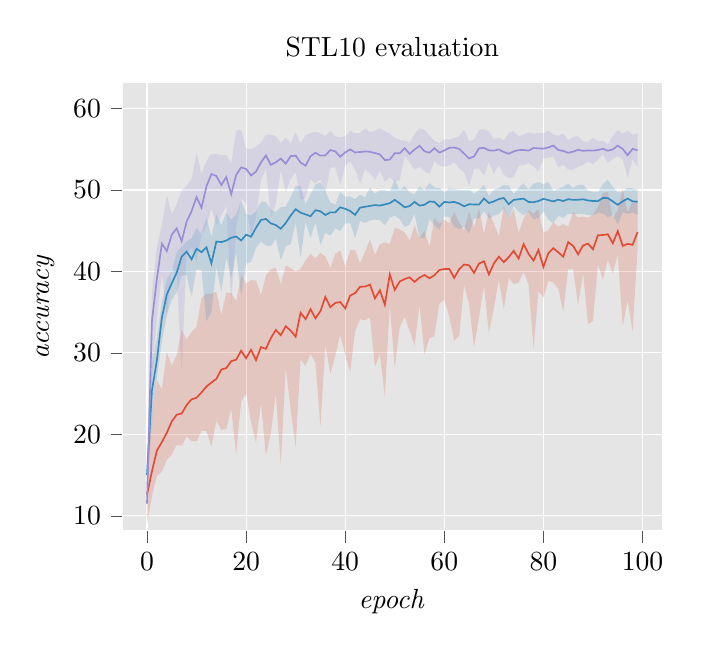
\begin{tikzpicture}

\definecolor{color0}{rgb}{0.886274509803922,0.290196078431373,0.2}
\definecolor{color1}{rgb}{0.203921568627451,0.541176470588235,0.741176470588235}
\definecolor{color2}{rgb}{0.596078431372549,0.556862745098039,0.835294117647059}

\begin{axis}[
axis background/.style={fill=white!89.8039215686275!black},
axis line style={white},
legend cell align={left},
legend style={fill opacity=0.8, draw opacity=1, text opacity=1, at={(0.97,0.03)}, anchor=south east, draw=white!80!black, fill=white!89.8039215686275!black},
log basis y={10},
tick align=outside,
tick pos=left,
title={STL10 evaluation},
x grid style={white},
xlabel={\textit{epoch}},
xmajorgrids,
xmin=-4.95, xmax=103.95,
xtick style={color=white!33.3333333333333!black},
y grid style={white},
ylabel={\textit{accuracy}},
ymajorgrids,
ymin=8.15863803616345, ymax=63.2058278627682,
%ymode=log,
ytick style={color=white!33.3333333333333!black}
]
\path [fill=color0, fill opacity=0.2, very thin]
(axis cs:0,17.6282)
--(axis cs:0,8.95433)
--(axis cs:1,12.3798)
--(axis cs:2,14.9038)
--(axis cs:3,15.4247)
--(axis cs:4,16.867)
--(axis cs:5,17.508)
--(axis cs:6,18.73)
--(axis cs:7,18.5897)
--(axis cs:8,19.7516)
--(axis cs:9,19.1707)
--(axis cs:10,19.1306)
--(axis cs:11,20.4527)
--(axis cs:12,20.3926)
--(axis cs:13,18.4896)
--(axis cs:14,21.6747)
--(axis cs:15,20.5529)
--(axis cs:16,20.6731)
--(axis cs:17,23.0769)
--(axis cs:18,17.528)
--(axis cs:19,24.0585)
--(axis cs:20,25.02)
--(axis cs:21,21.4944)
--(axis cs:22,18.9704)
--(axis cs:23,23.7981)
--(axis cs:24,17.4279)
--(axis cs:25,20.1723)
--(axis cs:26,24.9599)
--(axis cs:27,16.246)
--(axis cs:28,28.145)
--(axis cs:29,23.0369)
--(axis cs:30,18.4095)
--(axis cs:31,29.1867)
--(axis cs:32,28.4054)
--(axis cs:33,29.9079)
--(axis cs:34,28.7861)
--(axis cs:35,20.9535)
--(axis cs:36,30.9896)
--(axis cs:37,27.4038)
--(axis cs:38,29.6875)
--(axis cs:39,32.2316)
--(axis cs:40,29.7676)
--(axis cs:41,27.6843)
--(axis cs:42,32.6322)
--(axis cs:43,34.1346)
--(axis cs:44,33.9944)
--(axis cs:45,34.375)
--(axis cs:46,28.2652)
--(axis cs:47,29.8678)
--(axis cs:48,24.5994)
--(axis cs:49,35.9375)
--(axis cs:50,28.0849)
--(axis cs:51,33.133)
--(axis cs:52,34.4151)
--(axis cs:53,32.7324)
--(axis cs:54,30.9095)
--(axis cs:55,35.8574)
--(axis cs:56,29.7877)
--(axis cs:57,31.8109)
--(axis cs:58,32.0312)
--(axis cs:59,36.0577)
--(axis cs:60,36.5585)
--(axis cs:61,34.4551)
--(axis cs:62,31.5104)
--(axis cs:63,32.1114)
--(axis cs:64,38.3213)
--(axis cs:65,35.9175)
--(axis cs:66,30.7492)
--(axis cs:67,34.355)
--(axis cs:68,38.2612)
--(axis cs:69,32.472)
--(axis cs:70,35.4968)
--(axis cs:71,38.9623)
--(axis cs:72,35.4167)
--(axis cs:73,39.2027)
--(axis cs:74,38.4615)
--(axis cs:75,38.6218)
--(axis cs:76,39.9639)
--(axis cs:77,38.4014)
--(axis cs:78,30.4688)
--(axis cs:79,37.6202)
--(axis cs:80,36.7588)
--(axis cs:81,38.8622)
--(axis cs:82,38.6418)
--(axis cs:83,37.8806)
--(axis cs:84,35.0761)
--(axis cs:85,40.2644)
--(axis cs:86,40.2845)
--(axis cs:87,35.8574)
--(axis cs:88,39.8037)
--(axis cs:89,33.5537)
--(axis cs:90,33.9143)
--(axis cs:91,40.9054)
--(axis cs:92,39.0224)
--(axis cs:93,41.4062)
--(axis cs:94,39.6835)
--(axis cs:95,42.0673)
--(axis cs:96,33.2933)
--(axis cs:97,36.4383)
--(axis cs:98,32.6522)
--(axis cs:99,42.7083)
--(axis cs:99,48.6979)
--(axis cs:99,48.6979)
--(axis cs:98,48.6779)
--(axis cs:97,47.1955)
--(axis cs:96,50.1402)
--(axis cs:95,47.516)
--(axis cs:94,46.6146)
--(axis cs:93,49.7796)
--(axis cs:92,49.6194)
--(axis cs:91,47.9167)
--(axis cs:90,46.9952)
--(axis cs:89,46.5946)
--(axis cs:88,46.7348)
--(axis cs:87,46.6346)
--(axis cs:86,47.2756)
--(axis cs:85,45.5128)
--(axis cs:84,45.8333)
--(axis cs:83,45.4928)
--(axis cs:82,46.0537)
--(axis cs:81,45.0521)
--(axis cs:80,44.7516)
--(axis cs:79,47.6162)
--(axis cs:78,47.1154)
--(axis cs:77,47.516)
--(axis cs:76,46.5345)
--(axis cs:75,44.7316)
--(axis cs:74,47.6562)
--(axis cs:73,46.4744)
--(axis cs:72,48.0168)
--(axis cs:71,44.3109)
--(axis cs:70,45.9135)
--(axis cs:69,47.2957)
--(axis cs:68,44.6514)
--(axis cs:67,47.7163)
--(axis cs:66,45.3926)
--(axis cs:65,47.3758)
--(axis cs:64,45.0321)
--(axis cs:63,46.0337)
--(axis cs:62,47.3157)
--(axis cs:61,45.9135)
--(axis cs:60,46.3742)
--(axis cs:59,45.8534)
--(axis cs:58,46.5545)
--(axis cs:57,43.0489)
--(axis cs:56,45.0321)
--(axis cs:55,44.0505)
--(axis cs:54,45.653)
--(axis cs:53,43.7901)
--(axis cs:52,44.7917)
--(axis cs:51,45.1522)
--(axis cs:50,45.3926)
--(axis cs:49,43.3694)
--(axis cs:48,43.5897)
--(axis cs:47,43.3293)
--(axis cs:46,42.0272)
--(axis cs:45,43.9103)
--(axis cs:44,42.4479)
--(axis cs:43,40.9655)
--(axis cs:42,42.6482)
--(axis cs:41,42.6282)
--(axis cs:40,40.605)
--(axis cs:39,42.5681)
--(axis cs:38,42.1675)
--(axis cs:37,40.4647)
--(axis cs:36,41.847)
--(axis cs:35,42.2877)
--(axis cs:34,41.6266)
--(axis cs:33,42.1675)
--(axis cs:32,41.3662)
--(axis cs:31,40.3245)
--(axis cs:30,39.984)
--(axis cs:29,40.4247)
--(axis cs:28,40.7252)
--(axis cs:27,38.4215)
--(axis cs:26,40.4447)
--(axis cs:25,40.3045)
--(axis cs:24,39.5232)
--(axis cs:23,37.0793)
--(axis cs:22,38.8822)
--(axis cs:21,38.9623)
--(axis cs:20,38.5216)
--(axis cs:19,39.5833)
--(axis cs:18,36.3782)
--(axis cs:17,37.3397)
--(axis cs:16,37.4399)
--(axis cs:15,34.6755)
--(axis cs:14,37.52)
--(axis cs:13,37.2596)
--(axis cs:12,37.2796)
--(axis cs:11,36.7588)
--(axis cs:10,33.1931)
--(axis cs:9,32.5921)
--(axis cs:8,31.6707)
--(axis cs:7,32.8325)
--(axis cs:6,29.7877)
--(axis cs:5,28.4455)
--(axis cs:4,30.0881)
--(axis cs:3,25.5409)
--(axis cs:2,26.6426)
--(axis cs:1,21.7949)
--(axis cs:0,17.6282)
--cycle;

\path [fill=color1, fill opacity=0.2, very thin]
(axis cs:0,16.4062)
--(axis cs:0,12.9836)
--(axis cs:1,21.5526)
--(axis cs:2,26.9717)
--(axis cs:3,31.3988)
--(axis cs:4,34.7098)
--(axis cs:5,36.5203)
--(axis cs:6,37.4628)
--(axis cs:7,39.4717)
--(axis cs:8,39.5709)
--(axis cs:9,36.9048)
--(axis cs:10,40.2902)
--(axis cs:11,40.1166)
--(axis cs:12,33.8914)
--(axis cs:13,35.0074)
--(axis cs:14,40.5134)
--(axis cs:15,37.5248)
--(axis cs:16,41.7287)
--(axis cs:17,39.1245)
--(axis cs:18,42.3239)
--(axis cs:19,36.9916)
--(axis cs:20,40.9474)
--(axis cs:21,41.1706)
--(axis cs:22,42.8943)
--(axis cs:23,43.7004)
--(axis cs:24,43.1796)
--(axis cs:25,43.1176)
--(axis cs:26,44.0352)
--(axis cs:27,41.3938)
--(axis cs:28,43.0432)
--(axis cs:29,43.3656)
--(axis cs:30,45.9573)
--(axis cs:31,41.6915)
--(axis cs:32,46.0565)
--(axis cs:33,44.1096)
--(axis cs:34,46.0441)
--(axis cs:35,43.2664)
--(axis cs:36,44.7793)
--(axis cs:37,44.3824)
--(axis cs:38,45.3125)
--(axis cs:39,44.9529)
--(axis cs:40,45.8705)
--(axis cs:41,45.9697)
--(axis cs:42,44.0724)
--(axis cs:43,46.2054)
--(axis cs:44,45.9573)
--(axis cs:45,46.255)
--(axis cs:46,46.379)
--(axis cs:47,46.2798)
--(axis cs:48,45.6721)
--(axis cs:49,46.6146)
--(axis cs:50,46.8626)
--(axis cs:51,46.4286)
--(axis cs:52,45.4489)
--(axis cs:53,45.7713)
--(axis cs:54,47.061)
--(axis cs:55,44.1096)
--(axis cs:56,44.06)
--(axis cs:57,46.4286)
--(axis cs:58,45.6845)
--(axis cs:59,45.0893)
--(axis cs:60,46.7386)
--(axis cs:61,46.7138)
--(axis cs:62,45.4613)
--(axis cs:63,45.2009)
--(axis cs:64,45.5109)
--(axis cs:65,44.6677)
--(axis cs:66,46.503)
--(axis cs:67,46.4906)
--(axis cs:68,47.4082)
--(axis cs:69,46.4782)
--(axis cs:70,46.8626)
--(axis cs:71,47.0362)
--(axis cs:72,47.7679)
--(axis cs:73,46.5154)
--(axis cs:74,48.0655)
--(axis cs:75,47.3338)
--(axis cs:76,46.9246)
--(axis cs:77,47.3462)
--(axis cs:78,46.3914)
--(axis cs:79,46.565)
--(axis cs:80,47.371)
--(axis cs:81,46.3666)
--(axis cs:82,45.9449)
--(axis cs:83,46.813)
--(axis cs:84,46.5898)
--(axis cs:85,47.0982)
--(axis cs:86,47.0114)
--(axis cs:87,47.0858)
--(axis cs:88,47.061)
--(axis cs:89,46.937)
--(axis cs:90,46.8874)
--(axis cs:91,47.185)
--(axis cs:92,47.1478)
--(axis cs:93,46.627)
--(axis cs:94,46.9742)
--(axis cs:95,45.7713)
--(axis cs:96,47.247)
--(axis cs:97,47.0734)
--(axis cs:98,47.2346)
--(axis cs:99,46.937)
--(axis cs:99,50.062)
--(axis cs:99,50.062)
--(axis cs:98,50.2108)
--(axis cs:97,50.2976)
--(axis cs:96,49.8264)
--(axis cs:95,49.7148)
--(axis cs:94,50.3968)
--(axis cs:93,51.2401)
--(axis cs:92,50.7564)
--(axis cs:91,49.7272)
--(axis cs:90,49.7644)
--(axis cs:89,49.9628)
--(axis cs:88,50.6324)
--(axis cs:87,50.6572)
--(axis cs:86,50.2232)
--(axis cs:85,50.8061)
--(axis cs:84,50.4216)
--(axis cs:83,50.186)
--(axis cs:82,49.8636)
--(axis cs:81,50.9797)
--(axis cs:80,50.7068)
--(axis cs:79,50.9673)
--(axis cs:78,50.8061)
--(axis cs:77,50.0496)
--(axis cs:76,50.8433)
--(axis cs:75,50.2356)
--(axis cs:74,49.4916)
--(axis cs:73,50.5456)
--(axis cs:72,50.6076)
--(axis cs:71,50.2232)
--(axis cs:70,50.0248)
--(axis cs:69,49.2932)
--(axis cs:68,50.6324)
--(axis cs:67,50.0124)
--(axis cs:66,49.5536)
--(axis cs:65,50.0248)
--(axis cs:64,49.9752)
--(axis cs:63,50.0372)
--(axis cs:62,50.124)
--(axis cs:61,50.1984)
--(axis cs:60,49.7396)
--(axis cs:59,50.248)
--(axis cs:58,50.3224)
--(axis cs:57,50.8557)
--(axis cs:56,49.9628)
--(axis cs:55,50.4712)
--(axis cs:54,49.4544)
--(axis cs:53,49.7272)
--(axis cs:52,50.4836)
--(axis cs:51,49.9876)
--(axis cs:50,51.2773)
--(axis cs:49,49.8264)
--(axis cs:48,49.9752)
--(axis cs:47,50.0372)
--(axis cs:46,49.5288)
--(axis cs:45,50.3348)
--(axis cs:44,49.0699)
--(axis cs:43,49.4544)
--(axis cs:42,48.8839)
--(axis cs:41,49.2312)
--(axis cs:40,49.1815)
--(axis cs:39,49.7396)
--(axis cs:38,48.2143)
--(axis cs:37,48.4747)
--(axis cs:36,49.814)
--(axis cs:35,50.9301)
--(axis cs:34,50.6696)
--(axis cs:33,49.4792)
--(axis cs:32,48.2763)
--(axis cs:31,50.4712)
--(axis cs:30,50.5084)
--(axis cs:29,49.1443)
--(axis cs:28,47.9663)
--(axis cs:27,47.9167)
--(axis cs:26,47.309)
--(axis cs:25,47.5694)
--(axis cs:24,48.5367)
--(axis cs:23,48.5739)
--(axis cs:22,47.4082)
--(axis cs:21,46.8378)
--(axis cs:20,47.1106)
--(axis cs:19,48.7599)
--(axis cs:18,46.9866)
--(axis cs:17,46.3914)
--(axis cs:16,47.2098)
--(axis cs:15,45.7341)
--(axis cs:14,47.0238)
--(axis cs:13,44.2832)
--(axis cs:12,46.627)
--(axis cs:11,44.6305)
--(axis cs:10,45.3249)
--(axis cs:9,44.0848)
--(axis cs:8,43.7004)
--(axis cs:7,43.0804)
--(axis cs:6,42.4107)
--(axis cs:5,40.0546)
--(axis cs:4,38.9509)
--(axis cs:3,36.2847)
--(axis cs:2,31.8576)
--(axis cs:1,28.7946)
--(axis cs:0,16.4062)
--cycle;

\path [fill=color2, fill opacity=0.2, very thin]
(axis cs:0,17.559524)
--(axis cs:0,9.920635)
--(axis cs:1,27.157738)
--(axis cs:2,34.126984)
--(axis cs:3,39.657738)
--(axis cs:4,34.126984)
--(axis cs:5,40.562996)
--(axis cs:6,39.459325)
--(axis cs:7,27.641369)
--(axis cs:8,42.199901)
--(axis cs:9,42.906746)
--(axis cs:10,41.09623)
--(axis cs:11,44.53125)
--(axis cs:12,45.62252)
--(axis cs:13,47.730655)
--(axis cs:14,45.696925)
--(axis cs:15,46.875)
--(axis cs:16,48.040675)
--(axis cs:17,35.900298)
--(axis cs:18,45.337302)
--(axis cs:19,48.970734)
--(axis cs:20,48.375496)
--(axis cs:21,44.419643)
--(axis cs:22,46.540179)
--(axis cs:23,51.202877)
--(axis cs:24,52.616567)
--(axis cs:25,46.701389)
--(axis cs:26,48.338294)
--(axis cs:27,52.405754)
--(axis cs:28,49.739583)
--(axis cs:29,51.364087)
--(axis cs:30,52.18254)
--(axis cs:31,48.797123)
--(axis cs:32,49.007937)
--(axis cs:33,51.326885)
--(axis cs:34,50.830853)
--(axis cs:35,51.339286)
--(axis cs:36,49.553571)
--(axis cs:37,52.752976)
--(axis cs:38,52.790179)
--(axis cs:39,50.669643)
--(axis cs:40,52.97619)
--(axis cs:41,53.509425)
--(axis cs:42,52.542163)
--(axis cs:43,50.818452)
--(axis cs:44,52.554563)
--(axis cs:45,52.070933)
--(axis cs:46,51.25248)
--(axis cs:47,52.34375)
--(axis cs:48,51.016865)
--(axis cs:49,51.550099)
--(axis cs:50,51.066468)
--(axis cs:51,51.153274)
--(axis cs:52,54.154266)
--(axis cs:53,53.397817)
--(axis cs:54,52.480159)
--(axis cs:55,52.839782)
--(axis cs:56,52.281746)
--(axis cs:57,51.984127)
--(axis cs:58,53.509425)
--(axis cs:59,53.013393)
--(axis cs:60,52.864583)
--(axis cs:61,53.025794)
--(axis cs:62,53.410218)
--(axis cs:63,52.666171)
--(axis cs:64,52.157738)
--(axis cs:65,50.508433)
--(axis cs:66,52.641369)
--(axis cs:67,52.628968)
--(axis cs:68,51.72371)
--(axis cs:69,53.410218)
--(axis cs:70,51.984127)
--(axis cs:71,53.062996)
--(axis cs:72,51.87252)
--(axis cs:73,51.500496)
--(axis cs:74,51.5625)
--(axis cs:75,52.96379)
--(axis cs:76,53.062996)
--(axis cs:77,53.311012)
--(axis cs:78,52.926587)
--(axis cs:79,52.294147)
--(axis cs:80,53.856647)
--(axis cs:81,53.955853)
--(axis cs:82,54.154266)
--(axis cs:83,52.790179)
--(axis cs:84,53.075397)
--(axis cs:85,52.517361)
--(axis cs:86,52.442956)
--(axis cs:87,52.876984)
--(axis cs:88,53.050595)
--(axis cs:89,53.459821)
--(axis cs:90,53.174603)
--(axis cs:91,53.732639)
--(axis cs:92,54.389881)
--(axis cs:93,53.323413)
--(axis cs:94,53.769841)
--(axis cs:95,54.141865)
--(axis cs:96,53.769841)
--(axis cs:97,51.438492)
--(axis cs:98,53.769841)
--(axis cs:99,52.839782)
--(axis cs:99,57.056052)
--(axis cs:99,57.056052)
--(axis cs:98,56.783234)
--(axis cs:97,57.328869)
--(axis cs:96,56.919643)
--(axis cs:95,57.390873)
--(axis cs:94,56.646825)
--(axis cs:93,55.61756)
--(axis cs:92,56.076389)
--(axis cs:91,56.026786)
--(axis cs:90,56.460813)
--(axis cs:89,55.902778)
--(axis cs:88,55.989583)
--(axis cs:87,56.597222)
--(axis cs:86,56.535218)
--(axis cs:85,56.163194)
--(axis cs:84,56.932044)
--(axis cs:83,56.671627)
--(axis cs:82,56.795635)
--(axis cs:81,57.328869)
--(axis cs:80,56.969246)
--(axis cs:79,57.018849)
--(axis cs:78,56.932044)
--(axis cs:77,57.093254)
--(axis cs:76,56.820437)
--(axis cs:75,56.646825)
--(axis cs:74,57.254464)
--(axis cs:73,56.994048)
--(axis cs:72,56.125992)
--(axis cs:71,56.436012)
--(axis cs:70,56.25)
--(axis cs:69,57.217262)
--(axis cs:68,57.477679)
--(axis cs:67,57.390873)
--(axis cs:66,56.187996)
--(axis cs:65,56.001984)
--(axis cs:64,57.428075)
--(axis cs:63,56.56002)
--(axis cs:62,56.39881)
--(axis cs:61,56.212798)
--(axis cs:60,56.225198)
--(axis cs:59,55.741567)
--(axis cs:58,56.076389)
--(axis cs:57,56.696429)
--(axis cs:56,57.366071)
--(axis cs:55,57.589286)
--(axis cs:54,56.87004)
--(axis cs:53,55.803571)
--(axis cs:52,56.08879)
--(axis cs:51,56.175595)
--(axis cs:50,56.41121)
--(axis cs:49,56.932044)
--(axis cs:48,57.217262)
--(axis cs:47,57.576885)
--(axis cs:46,57.291667)
--(axis cs:45,57.105655)
--(axis cs:44,57.576885)
--(axis cs:43,56.994048)
--(axis cs:42,56.981647)
--(axis cs:41,57.254464)
--(axis cs:40,56.584821)
--(axis cs:39,56.473214)
--(axis cs:38,56.597222)
--(axis cs:37,57.291667)
--(axis cs:36,56.659226)
--(axis cs:35,56.944444)
--(axis cs:34,57.18006)
--(axis cs:33,56.969246)
--(axis cs:32,56.733631)
--(axis cs:31,55.753968)
--(axis cs:30,57.105655)
--(axis cs:29,55.716766)
--(axis cs:28,56.460813)
--(axis cs:27,55.766369)
--(axis cs:26,56.646825)
--(axis cs:25,56.783234)
--(axis cs:24,56.808036)
--(axis cs:23,55.803571)
--(axis cs:22,55.332341)
--(axis cs:21,54.985119)
--(axis cs:20,55.109127)
--(axis cs:19,57.390873)
--(axis cs:18,57.291667)
--(axis cs:17,53.28621)
--(axis cs:16,54.340278)
--(axis cs:15,54.265873)
--(axis cs:14,54.451885)
--(axis cs:13,54.427083)
--(axis cs:12,53.583829)
--(axis cs:11,51.946925)
--(axis cs:10,54.551091)
--(axis cs:9,51.364087)
--(axis cs:8,50.520833)
--(axis cs:7,49.987599)
--(axis cs:6,48.301091)
--(axis cs:5,47.085813)
--(axis cs:4,49.305556)
--(axis cs:3,45.758929)
--(axis cs:2,42.993552)
--(axis cs:1,37.475198)
--(axis cs:0,17.559524)
--cycle;

\addplot [semithick, color0]
table {%
0 12.5921440124512
1 15.4647483825684
2 18.0088024139404
3 19.0444927215576
4 20.1862983703613
5 21.5905494689941
6 22.4138793945312
7 22.5560913085938
8 23.6037673950195
9 24.3089065551758
10 24.4911861419678
11 25.1522426605225
12 25.8713893890381
13 26.3681926727295
14 26.8128986358643
15 27.9627380371094
16 28.1390209197998
17 28.9903736114502
18 29.1686515808105
19 30.2704257965088
20 29.3529644012451
21 30.3805866241455
22 29.1145935058594
23 30.7211513519287
24 30.504810333252
25 31.8329238891602
26 32.8225288391113
27 32.1674652099609
28 33.285270690918
29 32.7383804321289
30 31.9991912841797
31 34.9319000244141
32 34.1586494445801
33 35.3806266784668
34 34.244800567627
35 35.1462326049805
36 36.8769950866699
37 35.6129608154297
38 36.1418151855469
39 36.2439956665039
40 35.4727554321289
41 37.0372543334961
42 37.3477401733398
43 38.1250038146973
44 38.147029876709
45 38.3894348144531
46 36.6967124938965
47 37.6943130493164
48 35.9114646911621
49 39.6414184570312
50 37.736385345459
51 38.7740173339844
52 39.0685157775879
53 39.2828598022461
54 38.7199554443359
55 39.2548027038574
56 39.563304901123
57 39.1686553955078
58 39.5412750244141
59 40.178295135498
60 40.3084869384766
61 40.3125038146973
62 39.2187347412109
63 40.2824630737305
64 40.861385345459
65 40.7632179260254
66 39.8317489624023
67 40.9695625305176
68 41.2499961853027
69 39.6334228515625
70 40.9875946044922
71 41.8169136047363
72 41.1478462219238
73 41.7568092346191
74 42.5320434570312
75 41.58251953125
76 43.3653907775879
77 42.1574172973633
78 41.3541717529297
79 42.6342010498047
80 40.5629043579102
81 42.255615234375
82 42.8505554199219
83 42.3497505187988
84 41.8088760375977
85 43.5997543334961
86 43.1390228271484
87 42.1133766174316
88 43.2031173706055
89 43.4194755554199
90 42.7303771972656
91 44.4451179504395
92 44.4811706542969
93 44.5693016052246
94 43.4555320739746
95 44.9579391479492
96 43.1410331726074
97 43.3954429626465
98 43.271240234375
99 44.8457450866699
};
%\addlegendentry{cudnn}
\addplot [semithick, color1]
table {%
0 15.0198402404785
1 25.394344329834
2 29.0972175598145
3 34.3043174743652
4 37.168888092041
5 38.5528182983398
6 39.8635902404785
7 41.8278732299805
8 42.429313659668
9 41.4980278015137
10 42.7864761352539
11 42.3797149658203
12 42.9724655151367
13 40.9945259094238
14 43.6718711853027
15 43.6098556518555
16 43.7983551025391
17 44.1530303955078
18 44.2956275939941
19 43.8070487976074
20 44.5151252746582
21 44.2708320617676
22 45.3620834350586
23 46.324405670166
24 46.4508972167969
25 45.9089813232422
26 45.6981506347656
27 45.2480201721191
28 45.9548759460449
29 46.8675575256348
30 47.6450843811035
31 47.2259140014648
33 46.7894439697266
34 47.5260391235352
35 47.3995628356934
36 46.933292388916
37 47.2594223022461
38 47.2631454467773
39 47.8807029724121
40 47.6984062194824
41 47.4206314086914
42 46.9506492614746
43 47.8398094177246
46 48.1572456359863
47 48.0915145874023
49 48.386661529541
50 48.7946548461914
51 48.3655853271484
52 47.8794555664062
53 48.0356979370117
54 48.5478744506836
55 48.090274810791
56 48.1894836425781
57 48.5962448120117
58 48.5453948974609
59 47.9575843811035
60 48.5416793823242
61 48.477180480957
62 48.5429039001465
63 48.3395347595215
64 48.0071868896484
65 48.2539710998535
67 48.2118034362793
68 48.9670143127441
69 48.4065055847168
70 48.6086235046387
71 48.8901252746582
72 49.0277786254883
73 48.2713279724121
74 48.7909317016602
76 48.944694519043
77 48.5379486083984
78 48.5069427490234
79 48.6495513916016
80 48.9186248779297
82 48.6073989868164
83 48.8182067871094
84 48.6507911682129
85 48.8752593994141
86 48.7921524047852
87 48.8082656860352
88 48.8616027832031
89 48.7177543640137
90 48.6557464599609
91 48.6371612548828
92 49.0277633666992
93 49.0104217529297
95 48.1907424926758
96 48.6197929382324
97 48.9508857727051
98 48.612361907959
99 48.5652160644531
};
%\addlegendentry{libtorch}
\addplot [semithick, color2]
table {%
0 11.4918165206909
1 33.9298133850098
2 39.0959777832031
3 43.4102172851562
4 42.5123977661133
5 44.5250473022461
6 45.2988624572754
7 43.7214813232422
8 46.1185569763184
9 47.4045219421387
10 49.1331825256348
11 47.8286209106445
12 50.4464302062988
13 51.9568481445312
14 51.7299156188965
15 50.613842010498
16 51.5922660827637
17 49.4903297424316
18 51.8477210998535
19 52.7864532470703
20 52.5830841064453
21 51.7881965637207
22 52.2681121826172
23 53.3916091918945
24 54.2447967529297
25 53.0952377319336
26 53.4226150512695
27 53.8554077148438
28 53.2490119934082
29 54.1679153442383
30 54.2261848449707
31 53.3792152404785
32 52.9898262023926
33 54.1505508422852
34 54.5808486938477
35 54.2249488830566
36 54.2571830749512
37 54.9045143127441
38 54.7519836425781
39 54.0910263061523
40 54.6180610656738
41 54.9888381958008
42 54.6068916320801
44 54.7371063232422
45 54.6961822509766
47 54.3836860656738
48 53.6706275939941
49 53.7425537109375
50 54.5138893127441
51 54.5151329040527
52 55.1475677490234
53 54.4345207214355
54 54.9801597595215
55 55.4303169250488
56 54.7643852233887
57 54.5820922851562
58 55.1314506530762
59 54.604419708252
60 54.8561592102051
61 55.1909675598145
62 55.2170181274414
63 55.0545654296875
65 53.8727645874023
66 54.1306953430176
67 55.1178169250488
68 55.187255859375
69 54.8722724914551
70 54.8375511169434
71 54.9876022338867
72 54.6664161682129
73 54.4580917358398
74 54.7445449829102
75 54.9045143127441
76 54.9144325256348
77 54.8449859619141
78 55.1587257385254
80 55.0806121826172
81 55.2368621826172
82 55.4575881958008
83 54.9256019592285
84 54.7966232299805
85 54.5684432983398
86 54.7172622680664
87 54.9330368041992
88 54.8139839172363
89 54.863597869873
90 54.8363151550293
91 54.9131965637207
92 55.0681991577148
93 54.8288650512695
94 54.9888381958008
95 55.4600677490234
96 55.0458793640137
97 54.2757873535156
98 55.0620002746582
99 54.8598785400391
};
%\addlegendentry{pytorch}
\end{axis}

\end{tikzpicture}

    \end{figure}


    \begin{figure}
        % This file was created by tikzplotlib v0.9.5.
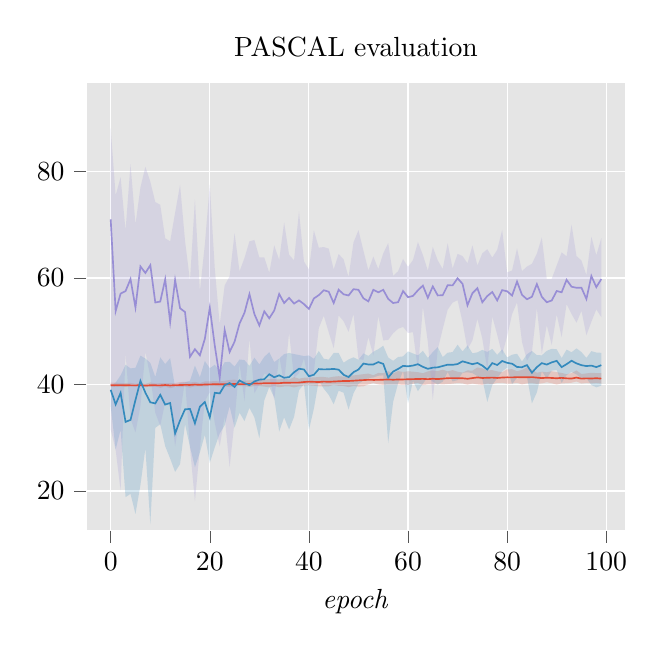
\begin{tikzpicture}

\definecolor{color0}{rgb}{0.886274509803922,0.290196078431373,0.2}
\definecolor{color1}{rgb}{0.203921568627451,0.541176470588235,0.741176470588235}
\definecolor{color2}{rgb}{0.596078431372549,0.556862745098039,0.835294117647059}

\begin{axis}[
axis background/.style={fill=white!89.8039215686275!black},
axis line style={white},
legend cell align={left},
legend style={fill opacity=0.8, draw opacity=1, text opacity=1, draw=white!80!black, fill=white!89.8039215686275!black},
log basis y={10},
tick align=outside,
tick pos=left,
title={PASCAL evaluation},
x grid style={white},
xlabel={\textit{epoch}},
xmajorgrids,
xmin=-4.95, xmax=103.95,
xtick style={color=white!33.3333333333333!black},
y grid style={white},
%ylabel={accuracy},
ymajorgrids,
ymin=12.524687588205, ymax=96.7215659804425,
%ymode=log,
ytick style={color=white!33.3333333333333!black}
]
\path [fill=color0, fill opacity=0.2, very thin]
(axis cs:0,40.3329)
--(axis cs:0,39.632)
--(axis cs:1,39.5444)
--(axis cs:2,39.6904)
--(axis cs:3,39.5444)
--(axis cs:4,39.6904)
--(axis cs:5,39.5736)
--(axis cs:6,39.7488)
--(axis cs:7,39.5152)
--(axis cs:8,39.5736)
--(axis cs:9,39.6612)
--(axis cs:10,39.3692)
--(axis cs:11,39.6028)
--(axis cs:12,39.3107)
--(axis cs:13,39.5444)
--(axis cs:14,39.5152)
--(axis cs:15,39.6028)
--(axis cs:16,39.4276)
--(axis cs:17,39.6612)
--(axis cs:18,39.632)
--(axis cs:19,39.6612)
--(axis cs:20,39.7488)
--(axis cs:21,39.778)
--(axis cs:22,39.632)
--(axis cs:23,39.632)
--(axis cs:24,39.5152)
--(axis cs:25,39.7196)
--(axis cs:26,39.7196)
--(axis cs:27,39.6904)
--(axis cs:28,39.5444)
--(axis cs:29,39.7196)
--(axis cs:30,39.7196)
--(axis cs:31,39.6028)
--(axis cs:32,39.486)
--(axis cs:33,39.7196)
--(axis cs:34,39.486)
--(axis cs:35,39.632)
--(axis cs:36,39.6612)
--(axis cs:37,39.4568)
--(axis cs:38,39.6612)
--(axis cs:39,39.8072)
--(axis cs:40,39.8364)
--(axis cs:41,39.778)
--(axis cs:42,39.6612)
--(axis cs:43,39.632)
--(axis cs:44,39.6612)
--(axis cs:45,39.9241)
--(axis cs:46,39.7488)
--(axis cs:47,39.7196)
--(axis cs:48,39.5152)
--(axis cs:49,39.7196)
--(axis cs:50,39.6028)
--(axis cs:51,39.6612)
--(axis cs:52,40.0117)
--(axis cs:53,40.2745)
--(axis cs:54,40.0117)
--(axis cs:55,39.9241)
--(axis cs:56,39.9825)
--(axis cs:57,39.9825)
--(axis cs:58,39.9825)
--(axis cs:59,39.9241)
--(axis cs:60,39.9241)
--(axis cs:61,40.1285)
--(axis cs:62,40.3037)
--(axis cs:63,39.8657)
--(axis cs:64,40.0117)
--(axis cs:65,40.0117)
--(axis cs:66,40.0993)
--(axis cs:67,40.0117)
--(axis cs:68,40.0993)
--(axis cs:69,40.1577)
--(axis cs:70,40.2745)
--(axis cs:71,40.2161)
--(axis cs:72,39.9533)
--(axis cs:73,40.1869)
--(axis cs:74,40.0117)
--(axis cs:75,39.9241)
--(axis cs:76,40.1869)
--(axis cs:77,40.0701)
--(axis cs:78,40.3037)
--(axis cs:79,40.3329)
--(axis cs:80,40.1577)
--(axis cs:81,40.1869)
--(axis cs:82,40.3329)
--(axis cs:83,40.0117)
--(axis cs:84,40.2161)
--(axis cs:85,40.2745)
--(axis cs:86,40.1285)
--(axis cs:87,40.2161)
--(axis cs:88,40.4206)
--(axis cs:89,40.2453)
--(axis cs:90,39.9825)
--(axis cs:91,40.2161)
--(axis cs:92,40.2453)
--(axis cs:93,40.3329)
--(axis cs:94,40.5666)
--(axis cs:95,40.1869)
--(axis cs:96,40.3037)
--(axis cs:97,40.2161)
--(axis cs:98,40.3037)
--(axis cs:99,40.1869)
--(axis cs:99,42.1437)
--(axis cs:99,42.1437)
--(axis cs:98,42.1437)
--(axis cs:97,42.2021)
--(axis cs:96,42.0853)
--(axis cs:95,41.9685)
--(axis cs:94,42.6402)
--(axis cs:93,42.1437)
--(axis cs:92,41.9393)
--(axis cs:91,42.1729)
--(axis cs:90,42.3189)
--(axis cs:89,42.4942)
--(axis cs:88,42.2897)
--(axis cs:87,42.4065)
--(axis cs:86,42.2021)
--(axis cs:85,42.7862)
--(axis cs:84,43.2243)
--(axis cs:83,42.7278)
--(axis cs:82,42.4942)
--(axis cs:81,42.8738)
--(axis cs:80,42.8446)
--(axis cs:79,42.3189)
--(axis cs:78,42.465)
--(axis cs:77,42.6986)
--(axis cs:76,42.6402)
--(axis cs:75,43.0199)
--(axis cs:74,43.1951)
--(axis cs:73,42.611)
--(axis cs:72,42.6402)
--(axis cs:71,42.2313)
--(axis cs:70,42.4065)
--(axis cs:69,42.6986)
--(axis cs:68,42.465)
--(axis cs:67,42.7862)
--(axis cs:66,42.5234)
--(axis cs:65,42.6402)
--(axis cs:64,42.465)
--(axis cs:63,42.1145)
--(axis cs:62,42.3189)
--(axis cs:61,42.4065)
--(axis cs:60,42.4942)
--(axis cs:59,42.3481)
--(axis cs:58,42.5234)
--(axis cs:57,42.0853)
--(axis cs:56,42.4942)
--(axis cs:55,42.1145)
--(axis cs:54,42.1729)
--(axis cs:53,41.7348)
--(axis cs:52,42.0561)
--(axis cs:51,41.9393)
--(axis cs:50,41.8224)
--(axis cs:49,41.7056)
--(axis cs:48,41.6472)
--(axis cs:47,41.472)
--(axis cs:46,41.5596)
--(axis cs:45,41.472)
--(axis cs:44,41.2967)
--(axis cs:43,41.4136)
--(axis cs:42,41.4136)
--(axis cs:41,41.3259)
--(axis cs:40,41.2967)
--(axis cs:39,41.2675)
--(axis cs:38,41.0923)
--(axis cs:37,41.3843)
--(axis cs:36,40.9171)
--(axis cs:35,41.1507)
--(axis cs:34,40.9463)
--(axis cs:33,41.0047)
--(axis cs:32,41.0339)
--(axis cs:31,40.9171)
--(axis cs:30,40.8294)
--(axis cs:29,40.771)
--(axis cs:28,40.8002)
--(axis cs:27,40.7126)
--(axis cs:26,40.6834)
--(axis cs:25,40.9171)
--(axis cs:24,40.8586)
--(axis cs:23,40.6834)
--(axis cs:22,40.5958)
--(axis cs:21,40.625)
--(axis cs:20,40.5958)
--(axis cs:19,40.5666)
--(axis cs:18,40.2745)
--(axis cs:17,40.5082)
--(axis cs:16,40.3621)
--(axis cs:15,40.5082)
--(axis cs:14,40.4498)
--(axis cs:13,40.2745)
--(axis cs:12,40.2745)
--(axis cs:11,40.2745)
--(axis cs:10,40.2453)
--(axis cs:9,40.2161)
--(axis cs:8,40.3914)
--(axis cs:7,40.0993)
--(axis cs:6,40.2745)
--(axis cs:5,40.1285)
--(axis cs:4,40.3037)
--(axis cs:3,40.2745)
--(axis cs:2,40.2745)
--(axis cs:1,40.3621)
--(axis cs:0,40.3329)
--cycle;

\path [fill=color1, fill opacity=0.2, very thin]
(axis cs:0,39.7569)
--(axis cs:0,35.9086)
--(axis cs:1,27.8067)
--(axis cs:2,31.4815)
--(axis cs:3,18.8368)
--(axis cs:4,19.4734)
--(axis cs:5,15.6829)
--(axis cs:6,21.0938)
--(axis cs:7,28.0093)
--(axis cs:8,13.7442)
--(axis cs:9,31.8576)
--(axis cs:10,32.5521)
--(axis cs:11,28.4144)
--(axis cs:12,26.0995)
--(axis cs:13,23.5822)
--(axis cs:14,25.0579)
--(axis cs:15,32.5521)
--(axis cs:16,28.3275)
--(axis cs:17,24.4502)
--(axis cs:18,27.2569)
--(axis cs:19,30.5556)
--(axis cs:20,25.2894)
--(axis cs:21,28.1829)
--(axis cs:22,30.787)
--(axis cs:23,32.3206)
--(axis cs:24,35.9086)
--(axis cs:25,31.8866)
--(axis cs:26,34.6933)
--(axis cs:27,33.1308)
--(axis cs:28,35.6192)
--(axis cs:29,33.8252)
--(axis cs:30,29.89)
--(axis cs:31,37.037)
--(axis cs:32,39.5255)
--(axis cs:33,37.5579)
--(axis cs:34,31.1632)
--(axis cs:35,33.8252)
--(axis cs:36,31.5394)
--(axis cs:37,33.912)
--(axis cs:38,38.9178)
--(axis cs:39,40.0463)
--(axis cs:40,31.4525)
--(axis cs:41,35.4456)
--(axis cs:42,40.7697)
--(axis cs:43,39.2072)
--(axis cs:44,38.0498)
--(axis cs:45,36.2847)
--(axis cs:46,38.831)
--(axis cs:47,38.4549)
--(axis cs:48,35.3009)
--(axis cs:49,38.3391)
--(axis cs:50,40.1331)
--(axis cs:51,40.7407)
--(axis cs:52,41.2037)
--(axis cs:53,41.3194)
--(axis cs:54,41.6377)
--(axis cs:55,41.7245)
--(axis cs:56,28.9931)
--(axis cs:57,36.7477)
--(axis cs:58,40.2199)
--(axis cs:59,42.5347)
--(axis cs:60,36.4873)
--(axis cs:61,40.6829)
--(axis cs:62,38.7442)
--(axis cs:63,40.1331)
--(axis cs:64,41.4352)
--(axis cs:65,40.5382)
--(axis cs:66,39.9884)
--(axis cs:67,40.5093)
--(axis cs:68,42.3322)
--(axis cs:69,40.5671)
--(axis cs:70,40.8275)
--(axis cs:71,42.1875)
--(axis cs:72,42.3032)
--(axis cs:73,42.1296)
--(axis cs:74,41.5799)
--(axis cs:75,41.0012)
--(axis cs:76,36.7188)
--(axis cs:77,39.9306)
--(axis cs:78,41.1748)
--(axis cs:79,42.4479)
--(axis cs:80,43.2002)
--(axis cs:81,40.0752)
--(axis cs:82,41.2905)
--(axis cs:83,41.3484)
--(axis cs:84,41.4352)
--(axis cs:85,36.4583)
--(axis cs:86,38.5127)
--(axis cs:87,42.4769)
--(axis cs:88,41.1458)
--(axis cs:89,42.5926)
--(axis cs:90,42.7373)
--(axis cs:91,40.3067)
--(axis cs:92,41.7824)
--(axis cs:93,42.3611)
--(axis cs:94,41.8981)
--(axis cs:95,41.1169)
--(axis cs:96,41.1748)
--(axis cs:97,39.9016)
--(axis cs:98,39.4676)
--(axis cs:99,39.7859)
--(axis cs:99,45.9491)
--(axis cs:99,45.9491)
--(axis cs:98,46.0069)
--(axis cs:97,46.2674)
--(axis cs:96,44.9942)
--(axis cs:95,46.0938)
--(axis cs:94,46.7882)
--(axis cs:93,46.0648)
--(axis cs:92,46.5567)
--(axis cs:91,44.9653)
--(axis cs:90,46.6146)
--(axis cs:89,46.7014)
--(axis cs:88,46.3252)
--(axis cs:87,45.4861)
--(axis cs:86,45.515)
--(axis cs:85,46.2963)
--(axis cs:84,45.6887)
--(axis cs:83,44.3287)
--(axis cs:82,45.7755)
--(axis cs:81,45.6019)
--(axis cs:80,45.081)
--(axis cs:79,46.6146)
--(axis cs:78,45.5729)
--(axis cs:77,46.7014)
--(axis cs:76,46.1227)
--(axis cs:75,46.4988)
--(axis cs:74,46.0359)
--(axis cs:73,45.8623)
--(axis cs:72,47.338)
--(axis cs:71,46.2095)
--(axis cs:70,47.4826)
--(axis cs:69,46.0938)
--(axis cs:68,45.978)
--(axis cs:67,45.1389)
--(axis cs:66,47.0197)
--(axis cs:65,46.0938)
--(axis cs:64,44.9942)
--(axis cs:63,46.3252)
--(axis cs:62,45.4861)
--(axis cs:61,45.8333)
--(axis cs:60,46.2095)
--(axis cs:59,45.2836)
--(axis cs:58,45.1678)
--(axis cs:57,44.4444)
--(axis cs:56,45.081)
--(axis cs:55,47.2801)
--(axis cs:54,46.6435)
--(axis cs:53,46.1516)
--(axis cs:52,45.3704)
--(axis cs:51,45.8333)
--(axis cs:50,44.647)
--(axis cs:49,45.11)
--(axis cs:48,44.7049)
--(axis cs:47,44.0972)
--(axis cs:46,45.9491)
--(axis cs:45,45.9201)
--(axis cs:44,44.6759)
--(axis cs:43,44.8495)
--(axis cs:42,46.2963)
--(axis cs:41,44.8206)
--(axis cs:40,45.4572)
--(axis cs:39,45.3414)
--(axis cs:38,45.544)
--(axis cs:37,45.7176)
--(axis cs:36,45.9201)
--(axis cs:35,45.7176)
--(axis cs:34,44.8785)
--(axis cs:33,44.213)
--(axis cs:32,46.0648)
--(axis cs:31,45.1968)
--(axis cs:30,43.7789)
--(axis cs:29,45.0521)
--(axis cs:28,43.4896)
--(axis cs:27,44.5891)
--(axis cs:26,44.7049)
--(axis cs:25,43.3738)
--(axis cs:24,44.2708)
--(axis cs:23,44.184)
--(axis cs:22,42.5926)
--(axis cs:21,43.7211)
--(axis cs:20,43.0556)
--(axis cs:19,44.4155)
--(axis cs:18,41.3773)
--(axis cs:17,43.5475)
--(axis cs:16,40.7118)
--(axis cs:15,40.4225)
--(axis cs:14,40.3067)
--(axis cs:13,39.4965)
--(axis cs:12,44.9653)
--(axis cs:11,43.8368)
--(axis cs:10,45.11)
--(axis cs:9,41.4352)
--(axis cs:8,44.0683)
--(axis cs:7,44.8785)
--(axis cs:6,45.4282)
--(axis cs:5,43.1424)
--(axis cs:4,43.0266)
--(axis cs:3,43.6921)
--(axis cs:2,41.7245)
--(axis cs:1,40.3646)
--(axis cs:0,39.7569)
--cycle;

\path [fill=color2, fill opacity=0.2, very thin]
(axis cs:0,88.139535)
--(axis cs:0,31.540698)
--(axis cs:1,27.703488)
--(axis cs:2,20.087209)
--(axis cs:3,45.872093)
--(axis cs:4,33.575581)
--(axis cs:5,30.988372)
--(axis cs:6,35.930233)
--(axis cs:7,46.104651)
--(axis cs:8,41.395349)
--(axis cs:9,34.680233)
--(axis cs:10,32.238372)
--(axis cs:11,36.627907)
--(axis cs:12,36.22093)
--(axis cs:13,28.372093)
--(axis cs:14,34.389535)
--(axis cs:15,40.755814)
--(axis cs:16,28.110465)
--(axis cs:17,18.052326)
--(axis cs:18,28.052326)
--(axis cs:19,36.889535)
--(axis cs:20,38.575581)
--(axis cs:21,32.790698)
--(axis cs:22,28.372093)
--(axis cs:23,34.011628)
--(axis cs:24,24.447674)
--(axis cs:25,33.168605)
--(axis cs:26,43.866279)
--(axis cs:27,36.860465)
--(axis cs:28,48.604651)
--(axis cs:29,38.343023)
--(axis cs:30,40)
--(axis cs:31,42.063953)
--(axis cs:32,41.686047)
--(axis cs:33,37.093023)
--(axis cs:34,45.319767)
--(axis cs:35,40.145349)
--(axis cs:36,49.680233)
--(axis cs:37,41.22093)
--(axis cs:38,42.151163)
--(axis cs:39,44.883721)
--(axis cs:40,40.523256)
--(axis cs:41,42.354651)
--(axis cs:42,50.581395)
--(axis cs:43,52.906977)
--(axis cs:44,49.796512)
--(axis cs:45,46.802326)
--(axis cs:46,52.965116)
--(axis cs:47,51.889535)
--(axis cs:48,49.883721)
--(axis cs:49,53.255814)
--(axis cs:50,44.796512)
--(axis cs:51,44.622093)
--(axis cs:52,48.866279)
--(axis cs:53,45.465116)
--(axis cs:54,52.848837)
--(axis cs:55,48.284884)
--(axis cs:56,48.372093)
--(axis cs:57,49.622093)
--(axis cs:58,50.465116)
--(axis cs:59,50.813953)
--(axis cs:60,49.680233)
--(axis cs:61,49.825581)
--(axis cs:62,42.645349)
--(axis cs:63,54.593023)
--(axis cs:64,47.994186)
--(axis cs:65,37.093023)
--(axis cs:66,46.569767)
--(axis cs:67,50.406977)
--(axis cs:68,54.040698)
--(axis cs:69,55.377907)
--(axis cs:70,55.843023)
--(axis cs:71,51.744186)
--(axis cs:72,46.598837)
--(axis cs:73,48.284884)
--(axis cs:74,52.325581)
--(axis cs:75,48.575581)
--(axis cs:76,42.761628)
--(axis cs:77,52.761628)
--(axis cs:78,49.360465)
--(axis cs:79,45.639535)
--(axis cs:80,49.069767)
--(axis cs:81,53.197674)
--(axis cs:82,55.436047)
--(axis cs:83,47.994186)
--(axis cs:84,44.476744)
--(axis cs:85,46.017442)
--(axis cs:86,54.331395)
--(axis cs:87,45.755814)
--(axis cs:88,51.133721)
--(axis cs:89,47.412791)
--(axis cs:90,53.168605)
--(axis cs:91,48.895349)
--(axis cs:92,55.087209)
--(axis cs:93,53.226744)
--(axis cs:94,51.598837)
--(axis cs:95,53.837209)
--(axis cs:96,49.244186)
--(axis cs:97,51.773256)
--(axis cs:98,54.098837)
--(axis cs:99,52.645349)
--(axis cs:99,67.5)
--(axis cs:99,67.5)
--(axis cs:98,64.273256)
--(axis cs:97,67.761628)
--(axis cs:96,60.552326)
--(axis cs:95,63.284884)
--(axis cs:94,64.127907)
--(axis cs:93,70.02907)
--(axis cs:92,64.069767)
--(axis cs:91,64.825581)
--(axis cs:90,62.354651)
--(axis cs:89,59.854651)
--(axis cs:88,59.825581)
--(axis cs:87,67.616279)
--(axis cs:86,64.593023)
--(axis cs:85,62.674419)
--(axis cs:84,62.151163)
--(axis cs:83,61.30814)
--(axis cs:82,65.581395)
--(axis cs:81,61.424419)
--(axis cs:80,61.046512)
--(axis cs:79,69.040698)
--(axis cs:78,65.290698)
--(axis cs:77,63.837209)
--(axis cs:76,65.406977)
--(axis cs:75,64.651163)
--(axis cs:74,62.354651)
--(axis cs:73,66.133721)
--(axis cs:72,62.761628)
--(axis cs:71,64.127907)
--(axis cs:70,64.534884)
--(axis cs:69,61.802326)
--(axis cs:68,66.540698)
--(axis cs:67,61.686047)
--(axis cs:66,63.313953)
--(axis cs:65,65.843023)
--(axis cs:64,61.395349)
--(axis cs:63,64.331395)
--(axis cs:62,66.773256)
--(axis cs:61,63.372093)
--(axis cs:60,62.093023)
--(axis cs:59,63.575581)
--(axis cs:58,61.27907)
--(axis cs:57,60.406977)
--(axis cs:56,66.569767)
--(axis cs:55,64.622093)
--(axis cs:54,61.686047)
--(axis cs:53,64.040698)
--(axis cs:52,61.424419)
--(axis cs:51,65.145349)
--(axis cs:50,68.982558)
--(axis cs:49,66.686047)
--(axis cs:48,60.174419)
--(axis cs:47,63.517442)
--(axis cs:46,64.505814)
--(axis cs:45,61.598837)
--(axis cs:44,65.523256)
--(axis cs:43,65.813953)
--(axis cs:42,65.697674)
--(axis cs:41,68.953488)
--(axis cs:40,61.598837)
--(axis cs:39,63.110465)
--(axis cs:38,72.5)
--(axis cs:37,63.313953)
--(axis cs:36,64.389535)
--(axis cs:35,70.436047)
--(axis cs:34,63.401163)
--(axis cs:33,66.133721)
--(axis cs:32,60.988372)
--(axis cs:31,63.866279)
--(axis cs:30,63.866279)
--(axis cs:29,67.151163)
--(axis cs:28,66.889535)
--(axis cs:27,63.77907)
--(axis cs:26,61.25)
--(axis cs:25,68.430233)
--(axis cs:24,60.319767)
--(axis cs:23,58.604651)
--(axis cs:22,51.30814)
--(axis cs:21,61.860465)
--(axis cs:20,77.52907)
--(axis cs:19,66.30814)
--(axis cs:18,57.55814)
--(axis cs:17,74.767442)
--(axis cs:16,59.505814)
--(axis cs:15,67.005814)
--(axis cs:14,77.5)
--(axis cs:13,72.267442)
--(axis cs:12,66.889535)
--(axis cs:11,67.47093)
--(axis cs:10,73.75)
--(axis cs:9,74.273256)
--(axis cs:8,78.081395)
--(axis cs:7,80.901163)
--(axis cs:6,77.005814)
--(axis cs:5,70.087209)
--(axis cs:4,81.395349)
--(axis cs:3,68.924419)
--(axis cs:2,78.953488)
--(axis cs:1,75.523256)
--(axis cs:0,88.139535)
--cycle;

\addplot [semithick, color0]
table {%
0 39.8569030761719
1 39.8773460388184
5 39.8335418701172
6 39.8715019226074
7 39.7984809875488
8 39.8598251342773
10 39.8364524841309
11 39.9036140441895
12 39.821834564209
13 39.8831596374512
14 39.8948631286621
15 39.9357414245605
16 39.9152908325195
17 39.9883270263672
18 39.9328155517578
19 39.9999961853027
21 40.0467414855957
23 40.0496559143066
24 40.0525703430176
25 40.0992774963379
26 40.0642356872559
28 40.0934448242188
29 40.1869087219238
30 40.1693649291992
31 40.2394943237305
34 40.2482452392578
35 40.3300247192383
38 40.3621520996094
39 40.4643630981445
40 40.5373687744141
42 40.4614639282227
43 40.5490646362305
44 40.5052452087402
47 40.6571159362793
48 40.6571273803711
50 40.7768592834473
52 40.882007598877
53 40.8586387634277
54 40.8674011230469
56 40.9433364868164
57 40.896598815918
58 40.9433555603027
59 40.9521255493164
61 41.0105056762695
63 41.0572509765625
64 41.0017509460449
65 41.0747680664062
66 41.019287109375
68 41.1857452392578
69 41.2032699584961
71 41.1769828796387
72 41.0776863098145
74 41.3317832946777
75 41.226634979248
77 41.2967529296875
78 41.2324829101562
79 41.308406829834
80 41.349292755127
81 41.3317832946777
82 41.3814239501953
84 41.3522071838379
85 41.3902053833008
87 41.2003440856934
88 41.2821083068848
90 41.1740798950195
91 41.2470741271973
92 41.1594696044922
93 41.112735748291
94 41.2996520996094
95 41.0981330871582
96 41.1594696044922
97 41.118579864502
98 41.1857452392578
99 41.1068878173828
};
%\addlegendentry{cudnn}
\addplot [semithick, color1]
table {%
0 39.0075225830078
1 36.2586708068848
2 38.4201316833496
3 32.9716300964355
4 33.3506965637207
5 37.0833473205566
6 40.6828727722168
7 38.463550567627
8 36.6493225097656
9 36.449634552002
10 38.0584526062012
11 36.2326354980469
12 36.5248794555664
13 30.7986106872559
14 33.2696762084961
15 35.3414344787598
16 35.4166488647461
17 32.7227935791016
18 35.8333320617676
19 36.7042999267578
20 33.8310394287109
21 38.4461784362793
22 38.3333206176758
23 39.8813743591309
24 40.2690849304199
25 39.5341453552246
26 40.7667770385742
27 40.2430534362793
28 39.8755950927734
29 40.5700073242188
30 40.9143257141113
31 40.9866943359375
32 41.9270858764648
33 41.3599739074707
34 41.7303161621094
35 41.2702484130859
36 41.3917846679688
37 42.2916679382324
38 42.9600715637207
39 42.8269538879395
40 41.548038482666
41 41.8315849304199
42 42.8964157104492
43 42.8356437683105
44 42.8645782470703
45 42.9282455444336
46 42.7864532470703
47 41.8258323669434
48 41.3975677490234
49 42.3148078918457
50 42.8125114440918
51 43.935188293457
52 43.7615928649902
53 43.7615699768066
54 44.2129669189453
55 43.8773155212402
56 41.3107643127441
57 42.4363250732422
58 42.919548034668
59 43.5011672973633
60 43.4172477722168
61 43.5561180114746
62 43.8194351196289
63 43.3159828186035
64 42.9484786987305
65 43.159725189209
66 43.2291564941406
68 43.7239646911621
69 43.6950149536133
70 43.8425941467285
71 44.3518486022949
73 43.8194351196289
74 44.0480308532715
75 43.5532493591309
76 42.8125114440918
77 44.0190963745117
78 43.6603164672852
79 44.4126052856445
80 44.0711555480957
81 43.9033508300781
82 43.2928161621094
83 43.2465438842773
84 43.6429443359375
85 42.2164268493652
86 43.255199432373
87 44.0162086486816
88 43.7413215637207
89 44.1579895019531
90 44.4415550231934
91 43.2609939575195
92 43.8223342895508
93 44.4560241699219
94 43.969898223877
95 43.628475189209
96 43.457763671875
97 43.5503578186035
98 43.2667655944824
99 43.6313743591309
};
%\addlegendentry{libtorch}
\addplot [semithick, color2]
table {%
0 71.0145263671875
1 53.7819862365723
2 57.0668640136719
3 57.5436134338379
4 59.7936019897461
5 54.468017578125
6 62.1831436157227
7 60.9505729675293
8 62.4156951904297
9 55.4040756225586
10 55.5755805969238
11 59.7499923706055
12 51.7296485900879
13 59.6220893859863
14 54.3284950256348
15 53.6075553894043
16 45.1976737976074
17 46.6308174133301
18 45.4767417907715
19 48.5842933654785
20 54.415699005127
21 47.3284873962402
22 41.2558174133301
23 50.2412757873535
24 46.1133804321289
25 48.0465087890625
26 51.4418640136719
27 53.4709243774414
28 56.9709396362305
29 53.2180213928223
30 51.0901107788086
31 53.7412872314453
32 52.4331474304199
33 53.8924331665039
34 56.9941825866699
35 55.3023223876953
36 56.2732620239258
37 55.2005729675293
38 55.7936058044434
39 55.1075592041016
40 54.1860427856445
41 56.1569747924805
42 56.7907028198242
43 57.7063903808594
44 57.4302368164062
45 55.3110504150391
46 57.8081398010254
47 56.9389533996582
48 56.7238349914551
49 57.9011688232422
50 57.7819786071777
51 56.1860389709473
52 55.6191825866699
53 57.7790603637695
54 57.3139533996582
55 57.7848815917969
56 56.0813865661621
57 55.3052368164062
58 55.4593086242676
59 57.5552406311035
60 56.3953399658203
61 56.6424446105957
62 57.6918678283691
63 58.5755882263184
64 56.2848930358887
65 58.4244194030762
66 56.7296600341797
67 56.767448425293
68 58.6366195678711
69 58.6191902160645
70 59.9505844116211
71 58.9098892211914
72 54.8866271972656
73 57.1569747924805
74 58.0842933654785
75 55.4476776123047
76 56.616283416748
77 57.3720970153809
78 55.7906951904297
79 57.726749420166
80 57.508716583252
81 56.7034873962402
82 59.3313941955566
83 56.8401222229004
84 56.0145263671875
85 56.4651222229004
86 58.8546447753906
87 56.4680213928223
88 55.4505844116211
89 55.7790718078613
90 57.5581474304199
91 57.3197593688965
92 59.6540603637695
93 58.366283416748
94 58.1656951904297
95 58.177318572998
96 56.0581321716309
97 60.3779106140137
98 58.2819786071777
99 59.802318572998
};
%\addlegendentry{pytorch}
\end{axis}

\end{tikzpicture}

    \end{figure}


    \begin{figure}
        % This file was created by tikzplotlib v0.9.5.
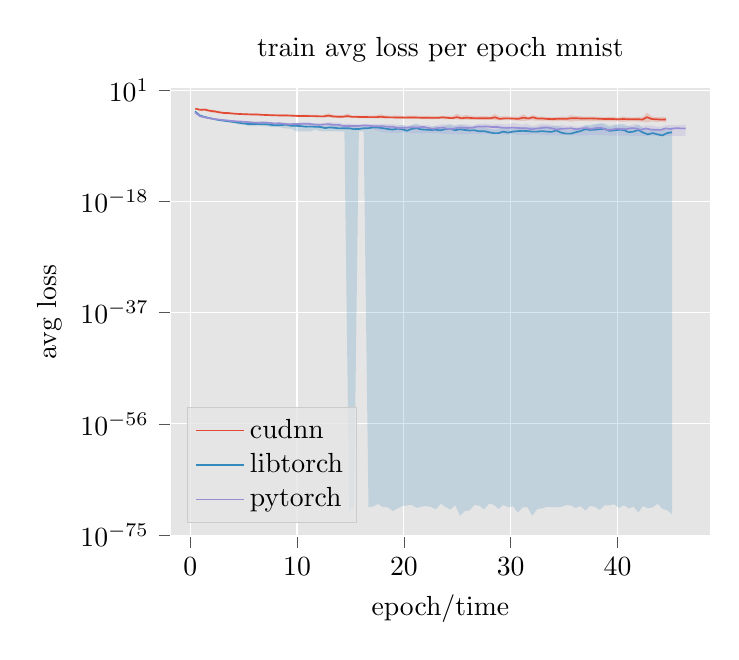
\begin{tikzpicture}

\definecolor{color0}{rgb}{0.886274509803922,0.290196078431373,0.2}
\definecolor{color1}{rgb}{0.203921568627451,0.541176470588235,0.741176470588235}
\definecolor{color2}{rgb}{0.596078431372549,0.556862745098039,0.835294117647059}

\begin{axis}[
axis background/.style={fill=white!89.8039215686275!black},
axis line style={white},
legend cell align={left},
legend style={fill opacity=0.8, draw opacity=1, text opacity=1, at={(0.03,0.03)}, anchor=south west, draw=white!80!black, fill=white!89.8039215686275!black},
log basis y={10},
tick align=outside,
tick pos=left,
title={train avg loss per epoch mnist},
x grid style={white},
xlabel={epoch/time},
xmajorgrids,
xmin=-1.8444581, xmax=48.6648733,
xtick style={color=white!33.3333333333333!black},
y grid style={white},
ylabel={avg loss},
ymajorgrids,
ymin=6.42533567318612e-76, ymax=26.6741291967659,
ymode=log,
ytick style={color=white!33.3333333333333!black}
]
\path [fill=color0, fill opacity=0.2, very thin]
(axis cs:0.4782266,0.007964)
--(axis cs:0.4782266,0.006996)
--(axis cs:0.9232159,0.0039)
--(axis cs:1.3681511,0.003101)
--(axis cs:1.813181,0.001997)
--(axis cs:2.2582623,0.00129)
--(axis cs:2.7032656,0.001147)
--(axis cs:3.1482741,0.000909)
--(axis cs:3.5932938,0.000773)
--(axis cs:4.038329,0.000919)
--(axis cs:4.4834467,0.000782)
--(axis cs:4.9285291,0.000685)
--(axis cs:5.3737088,0.000644)
--(axis cs:5.8189509,0.000588)
--(axis cs:6.2641013,0.000551)
--(axis cs:6.7093389,0.000509)
--(axis cs:7.1544196,0.000473)
--(axis cs:7.5995075,0.000433)
--(axis cs:8.0445662,0.000398)
--(axis cs:8.489797,0.000388)
--(axis cs:8.9349618,0.00037)
--(axis cs:9.3799734,0.000343)
--(axis cs:9.8251089,0.000322)
--(axis cs:10.2701673,0.000328)
--(axis cs:10.7152981,0.000312)
--(axis cs:11.1603761,0.000287)
--(axis cs:11.6055043,0.000291)
--(axis cs:12.0506865,0.00026)
--(axis cs:12.4958184,0.000243)
--(axis cs:12.9409165,0.000252)
--(axis cs:13.3859977,0.000222)
--(axis cs:13.8311519,0.000212)
--(axis cs:14.2761924,0.000203)
--(axis cs:14.7213617,0.000204)
--(axis cs:15.1664679,0.000201)
--(axis cs:15.6114732,0.000172)
--(axis cs:16.0566084,0.00019)
--(axis cs:16.501812,0.000166)
--(axis cs:16.9470843,0.000177)
--(axis cs:17.3922826,0.000166)
--(axis cs:17.8373712,0.000161)
--(axis cs:18.282443,0.000155)
--(axis cs:18.7275257,0.000162)
--(axis cs:19.1725744,0.000148)
--(axis cs:19.6176348,0.000128)
--(axis cs:20.0626668,0.000141)
--(axis cs:20.5078902,0.000134)
--(axis cs:20.9531108,0.000137)
--(axis cs:21.398351,0.000126)
--(axis cs:21.843595,0.000116)
--(axis cs:22.2887302,0.000123)
--(axis cs:22.7337989,0.000114)
--(axis cs:23.1789517,0.000123)
--(axis cs:23.6240882,0.000126)
--(axis cs:24.0692921,0.000116)
--(axis cs:24.5144183,0.000119)
--(axis cs:24.9595631,0.000107)
--(axis cs:25.4046424,9.9e-05)
--(axis cs:25.8497148,9.8e-05)
--(axis cs:26.2947474,9.2e-05)
--(axis cs:26.7398837,9.8e-05)
--(axis cs:27.1848716,8.9e-05)
--(axis cs:27.6299501,8.5e-05)
--(axis cs:28.0749458,9.7e-05)
--(axis cs:28.5199763,8.5e-05)
--(axis cs:28.9651299,7.7e-05)
--(axis cs:29.4101996,8.5e-05)
--(axis cs:29.8552906,7.8e-05)
--(axis cs:30.3002666,7.5e-05)
--(axis cs:30.7453382,6.5e-05)
--(axis cs:31.190327,6e-05)
--(axis cs:31.6354719,7.3e-05)
--(axis cs:32.0805844,7.2e-05)
--(axis cs:32.5257041,6.8e-05)
--(axis cs:32.9708542,6.3e-05)
--(axis cs:33.4160196,7.1e-05)
--(axis cs:33.8610718,5.1e-05)
--(axis cs:34.3061513,5.6e-05)
--(axis cs:34.7512437,6.6e-05)
--(axis cs:35.1961926,5.9e-05)
--(axis cs:35.6411077,4.4e-05)
--(axis cs:36.0860932,5.8e-05)
--(axis cs:36.5310712,6.1e-05)
--(axis cs:36.9761031,6.2e-05)
--(axis cs:37.4211117,5.1e-05)
--(axis cs:37.8660675,5.9e-05)
--(axis cs:38.3110037,5.1e-05)
--(axis cs:38.7560695,5e-05)
--(axis cs:39.2011195,5e-05)
--(axis cs:39.6460269,5.3e-05)
--(axis cs:40.0909067,4.7e-05)
--(axis cs:40.5359762,4.3e-05)
--(axis cs:40.9810362,4.9e-05)
--(axis cs:41.4260278,5.3e-05)
--(axis cs:41.8710576,4.8e-05)
--(axis cs:42.316014,4.2e-05)
--(axis cs:42.760984,3.3e-05)
--(axis cs:43.2059163,5.1e-05)
--(axis cs:43.6508853,3.8e-05)
--(axis cs:44.0959597,4.6e-05)
--(axis cs:44.5409831,3.5e-05)
--(axis cs:44.5409831,0.000269)
--(axis cs:44.5409831,0.000269)
--(axis cs:44.0959597,0.000295)
--(axis cs:43.6508853,0.000288)
--(axis cs:43.2059163,0.00034)
--(axis cs:42.760984,0.001593)
--(axis cs:42.316014,0.000254)
--(axis cs:41.8710576,0.000272)
--(axis cs:41.4260278,0.000232)
--(axis cs:40.9810362,0.000258)
--(axis cs:40.5359762,0.000355)
--(axis cs:40.0909067,0.000227)
--(axis cs:39.6460269,0.000284)
--(axis cs:39.2011195,0.000315)
--(axis cs:38.7560695,0.00026)
--(axis cs:38.3110037,0.000326)
--(axis cs:37.8660675,0.000324)
--(axis cs:37.4211117,0.000321)
--(axis cs:36.9761031,0.000308)
--(axis cs:36.5310712,0.000379)
--(axis cs:36.0860932,0.000433)
--(axis cs:35.6411077,0.000552)
--(axis cs:35.1961926,0.000308)
--(axis cs:34.7512437,0.000338)
--(axis cs:34.3061513,0.000284)
--(axis cs:33.8610718,0.000253)
--(axis cs:33.4160196,0.000281)
--(axis cs:32.9708542,0.000315)
--(axis cs:32.5257041,0.000345)
--(axis cs:32.0805844,0.000611)
--(axis cs:31.6354719,0.000302)
--(axis cs:31.190327,0.000847)
--(axis cs:30.7453382,0.00032)
--(axis cs:30.3002666,0.000329)
--(axis cs:29.8552906,0.000351)
--(axis cs:29.4101996,0.000407)
--(axis cs:28.9651299,0.000332)
--(axis cs:28.5199763,0.000936)
--(axis cs:28.0749458,0.000333)
--(axis cs:27.6299501,0.000415)
--(axis cs:27.1848716,0.000391)
--(axis cs:26.7398837,0.000355)
--(axis cs:26.2947474,0.000428)
--(axis cs:25.8497148,0.000656)
--(axis cs:25.4046424,0.000412)
--(axis cs:24.9595631,0.000974)
--(axis cs:24.5144183,0.000368)
--(axis cs:24.0692921,0.000419)
--(axis cs:23.6240882,0.00045)
--(axis cs:23.1789517,0.000439)
--(axis cs:22.7337989,0.000412)
--(axis cs:22.2887302,0.000457)
--(axis cs:21.843595,0.000416)
--(axis cs:21.398351,0.000455)
--(axis cs:20.9531108,0.000477)
--(axis cs:20.5078902,0.00051)
--(axis cs:20.0626668,0.000447)
--(axis cs:19.6176348,0.000459)
--(axis cs:19.1725744,0.000522)
--(axis cs:18.7275257,0.000465)
--(axis cs:18.282443,0.000518)
--(axis cs:17.8373712,0.000825)
--(axis cs:17.3922826,0.000548)
--(axis cs:16.9470843,0.00051)
--(axis cs:16.501812,0.000463)
--(axis cs:16.0566084,0.000488)
--(axis cs:15.6114732,0.000523)
--(axis cs:15.1664679,0.00049)
--(axis cs:14.7213617,0.001024)
--(axis cs:14.2761924,0.000553)
--(axis cs:13.8311519,0.000573)
--(axis cs:13.3859977,0.000652)
--(axis cs:12.9409165,0.001161)
--(axis cs:12.4958184,0.000662)
--(axis cs:12.0506865,0.000656)
--(axis cs:11.6055043,0.000709)
--(axis cs:11.1603761,0.000713)
--(axis cs:10.7152981,0.000702)
--(axis cs:10.2701673,0.000724)
--(axis cs:9.8251089,0.000741)
--(axis cs:9.3799734,0.000843)
--(axis cs:8.9349618,0.000831)
--(axis cs:8.489797,0.000868)
--(axis cs:8.0445662,0.000854)
--(axis cs:7.5995075,0.000887)
--(axis cs:7.1544196,0.00096)
--(axis cs:6.7093389,0.000975)
--(axis cs:6.2641013,0.001113)
--(axis cs:5.8189509,0.001147)
--(axis cs:5.3737088,0.001138)
--(axis cs:4.9285291,0.001156)
--(axis cs:4.4834467,0.001306)
--(axis cs:4.038329,0.001398)
--(axis cs:3.5932938,0.001826)
--(axis cs:3.1482741,0.002067)
--(axis cs:2.7032656,0.002716)
--(axis cs:2.2582623,0.004686)
--(axis cs:1.813181,0.005124)
--(axis cs:1.3681511,0.008779)
--(axis cs:0.9232159,0.005592)
--(axis cs:0.4782266,0.007964)
--cycle;

\path [fill=color1, fill opacity=0.2, very thin]
(axis cs:0.4514206,0.002729)
--(axis cs:0.4514206,0.002292)
--(axis cs:0.9022784,0.000486)
--(axis cs:1.3534231,0.000266)
--(axis cs:1.8043956,0.000159)
--(axis cs:2.255545,0.00011)
--(axis cs:2.7067402,7.1e-05)
--(axis cs:3.1576851,4.7e-05)
--(axis cs:3.6087245,4.1e-05)
--(axis cs:4.0595726,3.1e-05)
--(axis cs:4.5104858,1.5e-05)
--(axis cs:4.9615293,1.3e-05)
--(axis cs:5.4125489,9e-06)
--(axis cs:5.863595,8e-06)
--(axis cs:6.314577,1e-05)
--(axis cs:6.7656383,7e-06)
--(axis cs:7.2164882,7e-06)
--(axis cs:7.6673026,5e-06)
--(axis cs:8.1183483,6e-06)
--(axis cs:8.5693941,4e-06)
--(axis cs:9.0203725,3e-06)
--(axis cs:9.4712526,3e-06)
--(axis cs:9.9224924,1e-06)
--(axis cs:10.3732561,1e-06)
--(axis cs:10.8243106,1e-06)
--(axis cs:11.2752643,1e-06)
--(axis cs:11.7258814,2e-06)
--(axis cs:12.1768194,1e-06)
--(axis cs:12.6278308,1e-06)
--(axis cs:13.0786394,1e-06)
--(axis cs:13.529549,1e-06)
--(axis cs:13.9803709,1e-06)
--(axis cs:14.4313935,1e-06)
--(axis cs:14.8823161,7.79903790402995e-72)
--(axis cs:15.3333867,1.29271157857526e-70)
--(axis cs:15.7843831,1e-06)
--(axis cs:16.2350727,1e-06)
--(axis cs:16.6861017,5.84090495019293e-71)
--(axis cs:17.1369704,7.86612656815358e-71)
--(axis cs:17.5877198,2.00942926786625e-70)
--(axis cs:18.0386275,5.92198270593322e-71)
--(axis cs:18.489467,5.50365575967733e-71)
--(axis cs:18.9403415,1.27278001917643e-71)
--(axis cs:19.3913184,3.44841362840825e-71)
--(axis cs:19.8423633,9.2050903752056e-71)
--(axis cs:20.2933696,1.19826725893552e-70)
--(axis cs:20.7443091,1.50643450302719e-70)
--(axis cs:21.1955409,4.36659389777262e-71)
--(axis cs:21.6463799,7.35337978330449e-71)
--(axis cs:22.0973493,9.03785360890454e-71)
--(axis cs:22.548191,6.36176455230253e-71)
--(axis cs:22.9990786,2.37783233534397e-71)
--(axis cs:23.4500047,2.30137077700552e-70)
--(axis cs:23.9008287,6.27942226892779e-71)
--(axis cs:24.3516837,2.27957034186552e-71)
--(axis cs:24.80285,1.24594310100128e-70)
--(axis cs:25.2538591,2.01644550576756e-72)
--(axis cs:25.7046932,1.28954926879712e-71)
--(axis cs:26.1559451,1.69033218945265e-71)
--(axis cs:26.6070184,1.5086890278168e-70)
--(axis cs:27.0579189,1.08705603762124e-70)
--(axis cs:27.5088431,2.46798496676535e-71)
--(axis cs:27.9599997,2.34837631263401e-70)
--(axis cs:28.4110492,1.60877679885578e-70)
--(axis cs:28.8618921,2.98857972346276e-71)
--(axis cs:29.3128527,1.48979391956186e-70)
--(axis cs:29.7638637,5.60903813628843e-71)
--(axis cs:30.2149583,7.98596595747121e-71)
--(axis cs:30.6660081,7.18925662532147e-72)
--(axis cs:31.1165665,5.35828454021389e-71)
--(axis cs:31.5673747,5.30783410675106e-71)
--(axis cs:32.0183621,1.95227513246558e-72)
--(axis cs:32.4694334,2.7626859923811e-71)
--(axis cs:32.9205166,3.67128704821719e-71)
--(axis cs:33.3712593,6.40048809234656e-71)
--(axis cs:33.8220931,6.2748958933631e-71)
--(axis cs:34.2729178,5.81334112085947e-71)
--(axis cs:34.7240035,6.52681297580219e-71)
--(axis cs:35.1753118,1.33431128175969e-70)
--(axis cs:35.626446,1.1839284313765e-70)
--(axis cs:36.0774815,4.12445582462113e-71)
--(axis cs:36.5283737,8.88448537531756e-71)
--(axis cs:36.9791905,1.55120254437389e-71)
--(axis cs:37.4303597,9.62048854070251e-71)
--(axis cs:37.881495,6.61267383188287e-71)
--(axis cs:38.3325126,2.0403415875453e-71)
--(axis cs:38.7835199,1.1981330087916e-70)
--(axis cs:39.234442,1.28784695598028e-70)
--(axis cs:39.6855538,1.79068811339905e-70)
--(axis cs:40.1366098,4.32374683971766e-71)
--(axis cs:40.5878227,1.27642781211338e-70)
--(axis cs:41.0389411,3.59794912330991e-71)
--(axis cs:41.4898508,7.20820534756083e-71)
--(axis cs:41.9410489,7.2950977837235e-72)
--(axis cs:42.392293,9.51379267137364e-71)
--(axis cs:42.8432532,3.60296011807849e-71)
--(axis cs:43.2942657,5.63781602965244e-71)
--(axis cs:43.7452244,2.36909573889635e-70)
--(axis cs:44.1960269,2.98419095038784e-71)
--(axis cs:44.6471278,1.73433046300281e-71)
--(axis cs:45.0979666,3.72861220129379e-72)
--(axis cs:45.0979666,5e-06)
--(axis cs:45.0979666,5e-06)
--(axis cs:44.6471278,2e-06)
--(axis cs:44.1960269,2e-06)
--(axis cs:43.7452244,2e-06)
--(axis cs:43.2942657,3e-06)
--(axis cs:42.8432532,2e-06)
--(axis cs:42.392293,3e-06)
--(axis cs:41.9410489,1.4e-05)
--(axis cs:41.4898508,6e-06)
--(axis cs:41.0389411,7e-06)
--(axis cs:40.5878227,1.7e-05)
--(axis cs:40.1366098,1.7e-05)
--(axis cs:39.6855538,1.4e-05)
--(axis cs:39.234442,9e-06)
--(axis cs:38.7835199,2.3e-05)
--(axis cs:38.3325126,2.2e-05)
--(axis cs:37.881495,1.7e-05)
--(axis cs:37.4303597,1.3e-05)
--(axis cs:36.9791905,1.1e-05)
--(axis cs:36.5283737,3e-06)
--(axis cs:36.0774815,4e-06)
--(axis cs:35.626446,2e-06)
--(axis cs:35.1753118,2e-06)
--(axis cs:34.7240035,5e-06)
--(axis cs:34.2729178,1e-05)
--(axis cs:33.8220931,7e-06)
--(axis cs:33.3712593,7e-06)
--(axis cs:32.9205166,9e-06)
--(axis cs:32.4694334,4e-06)
--(axis cs:32.0183621,6e-06)
--(axis cs:31.5673747,5e-06)
--(axis cs:31.1165665,6e-06)
--(axis cs:30.6660081,4e-06)
--(axis cs:30.2149583,3e-06)
--(axis cs:29.7638637,5e-06)
--(axis cs:29.3128527,5e-06)
--(axis cs:28.8618921,3e-06)
--(axis cs:28.4110492,2e-06)
--(axis cs:27.9599997,3e-06)
--(axis cs:27.5088431,5e-06)
--(axis cs:27.0579189,5e-06)
--(axis cs:26.6070184,5e-06)
--(axis cs:26.1559451,7e-06)
--(axis cs:25.7046932,9e-06)
--(axis cs:25.2538591,1.3e-05)
--(axis cs:24.80285,7e-06)
--(axis cs:24.3516837,1.9e-05)
--(axis cs:23.9008287,1e-05)
--(axis cs:23.4500047,5e-06)
--(axis cs:22.9990786,8e-06)
--(axis cs:22.548191,6e-06)
--(axis cs:22.0973493,6e-06)
--(axis cs:21.6463799,7e-06)
--(axis cs:21.1955409,2.2e-05)
--(axis cs:20.7443091,1.2e-05)
--(axis cs:20.2933696,6e-06)
--(axis cs:19.8423633,1.2e-05)
--(axis cs:19.3913184,8e-06)
--(axis cs:18.9403415,5e-06)
--(axis cs:18.489467,8e-06)
--(axis cs:18.0386275,8e-06)
--(axis cs:17.5877198,1e-05)
--(axis cs:17.1369704,1.2e-05)
--(axis cs:16.6861017,9e-06)
--(axis cs:16.2350727,1.3e-05)
--(axis cs:15.7843831,7e-06)
--(axis cs:15.3333867,5e-06)
--(axis cs:14.8823161,8e-06)
--(axis cs:14.4313935,7e-06)
--(axis cs:13.9803709,9e-06)
--(axis cs:13.529549,1.4e-05)
--(axis cs:13.0786394,1.2e-05)
--(axis cs:12.6278308,7e-06)
--(axis cs:12.1768194,1.3e-05)
--(axis cs:11.7258814,1.6e-05)
--(axis cs:11.2752643,9e-06)
--(axis cs:10.8243106,1.5e-05)
--(axis cs:10.3732561,1.4e-05)
--(axis cs:9.9224924,1.5e-05)
--(axis cs:9.4712526,2e-05)
--(axis cs:9.0203725,2.8e-05)
--(axis cs:8.5693941,2.4e-05)
--(axis cs:8.1183483,2e-05)
--(axis cs:7.6673026,2.8e-05)
--(axis cs:7.2164882,3.1e-05)
--(axis cs:6.7656383,3.7e-05)
--(axis cs:6.314577,3e-05)
--(axis cs:5.863595,2.6e-05)
--(axis cs:5.4125489,2.6e-05)
--(axis cs:4.9615293,2.6e-05)
--(axis cs:4.5104858,4.2e-05)
--(axis cs:4.0595726,4.5e-05)
--(axis cs:3.6087245,6.4e-05)
--(axis cs:3.1576851,9.2e-05)
--(axis cs:2.7067402,9.9e-05)
--(axis cs:2.255545,0.000138)
--(axis cs:1.8043956,0.00021)
--(axis cs:1.3534231,0.000326)
--(axis cs:0.9022784,0.000566)
--(axis cs:0.4514206,0.002729)
--cycle;

\path [fill=color2, fill opacity=0.2, very thin]
(axis cs:0.4638433,0.0016304536)
--(axis cs:0.4638433,0.0015096476)
--(axis cs:0.9270713,0.0003472789)
--(axis cs:1.3897523,0.0002184277)
--(axis cs:1.852212,0.000148298)
--(axis cs:2.3150211,0.0001044754)
--(axis cs:2.7780984,8.99438e-05)
--(axis cs:3.241409,5.91701e-05)
--(axis cs:3.7050896,5.10774e-05)
--(axis cs:4.1685578,4.01416e-05)
--(axis cs:4.63141,3.94475e-05)
--(axis cs:5.0938514,3.04091e-05)
--(axis cs:5.5576098,1.9922e-05)
--(axis cs:6.0210603,1.87298e-05)
--(axis cs:6.4843292,2.06219e-05)
--(axis cs:6.9469475,2.48913e-05)
--(axis cs:7.4099499,1.86711e-05)
--(axis cs:7.8729495,1.203e-05)
--(axis cs:8.3352795,1.30723e-05)
--(axis cs:8.7984499,1.29668e-05)
--(axis cs:9.2620109,1.0515e-05)
--(axis cs:9.7251625,1.30447e-05)
--(axis cs:10.189057,7.2839e-06)
--(axis cs:10.6522043,1.28649e-05)
--(axis cs:11.1145413,6.1014e-06)
--(axis cs:11.5776748,7.8515e-06)
--(axis cs:12.0417346,3.7125e-06)
--(axis cs:12.5050999,5.489e-06)
--(axis cs:12.9679604,3.3827e-06)
--(axis cs:13.4318782,2.1804e-06)
--(axis cs:13.8947382,4.2191e-06)
--(axis cs:14.3589527,1.9696e-06)
--(axis cs:14.822034,1.7388e-06)
--(axis cs:15.2852567,3.5761e-06)
--(axis cs:15.7485038,4.3874e-06)
--(axis cs:16.2109994,2.3866e-06)
--(axis cs:16.6745642,2.2874e-06)
--(axis cs:17.1371118,2.2808e-06)
--(axis cs:17.6007818,1.1687e-06)
--(axis cs:18.0645292,6.559e-07)
--(axis cs:18.5272766,5.764e-07)
--(axis cs:18.9908405,5.633e-07)
--(axis cs:19.4532082,5.2e-07)
--(axis cs:19.9169471,6.211e-07)
--(axis cs:20.3807364,5.322e-07)
--(axis cs:20.8436679,4.226e-07)
--(axis cs:21.3063988,4.865e-07)
--(axis cs:21.7712675,4.501e-07)
--(axis cs:22.2339708,5.094e-07)
--(axis cs:22.6973071,4.375e-07)
--(axis cs:23.1602467,4.351e-07)
--(axis cs:23.6233873,3.57e-07)
--(axis cs:24.0868469,3.505e-07)
--(axis cs:24.5498423,3.32e-07)
--(axis cs:25.0130465,3.144e-07)
--(axis cs:25.4765129,3.029e-07)
--(axis cs:25.9406982,3.041e-07)
--(axis cs:26.4045968,3.551e-07)
--(axis cs:26.8673352,3.312e-07)
--(axis cs:27.3300115,3.223e-07)
--(axis cs:27.793151,3.329e-07)
--(axis cs:28.2555888,2.916e-07)
--(axis cs:28.719465,3.073e-07)
--(axis cs:29.1831128,2.87e-07)
--(axis cs:29.6455809,2.548e-07)
--(axis cs:30.1088232,3.808e-07)
--(axis cs:30.5729761,2.592e-07)
--(axis cs:31.0357632,2.415e-07)
--(axis cs:31.4984833,2.405e-07)
--(axis cs:31.9605774,2.95e-07)
--(axis cs:32.4237085,3.191e-07)
--(axis cs:32.8888928,2.496e-07)
--(axis cs:33.3517334,2.018e-07)
--(axis cs:33.8158782,2.162e-07)
--(axis cs:34.2791403,2.087e-07)
--(axis cs:34.7429744,2.08e-07)
--(axis cs:35.2075196,2.199e-07)
--(axis cs:35.67196,1.999e-07)
--(axis cs:36.1372871,2.022e-07)
--(axis cs:36.6032709,1.814e-07)
--(axis cs:37.0676407,2.103e-07)
--(axis cs:37.5321391,2.219e-07)
--(axis cs:37.9977197,2.227e-07)
--(axis cs:38.4633566,2.181e-07)
--(axis cs:38.9277333,2.057e-07)
--(axis cs:39.3923192,1.831e-07)
--(axis cs:39.8576905,1.826e-07)
--(axis cs:40.3227587,1.832e-07)
--(axis cs:40.7887013,1.949e-07)
--(axis cs:41.2535829,1.683e-07)
--(axis cs:41.717097,1.609e-07)
--(axis cs:42.1806705,1.691e-07)
--(axis cs:42.6455609,1.617e-07)
--(axis cs:43.1103244,1.699e-07)
--(axis cs:43.5752302,1.557e-07)
--(axis cs:44.0404622,1.658e-07)
--(axis cs:44.5061802,1.568e-07)
--(axis cs:44.9724253,1.541e-07)
--(axis cs:45.4374894,1.508e-07)
--(axis cs:45.9034288,1.667e-07)
--(axis cs:46.3689946,1.509e-07)
--(axis cs:46.3689946,1.41598e-05)
--(axis cs:46.3689946,1.41598e-05)
--(axis cs:45.9034288,1.18575e-05)
--(axis cs:45.4374894,1.16275e-05)
--(axis cs:44.9724253,1.30599e-05)
--(axis cs:44.5061802,1.07224e-05)
--(axis cs:44.0404622,6.0256e-06)
--(axis cs:43.5752302,7.0885e-06)
--(axis cs:43.1103244,1.06594e-05)
--(axis cs:42.6455609,1.0528e-05)
--(axis cs:42.1806705,7.6235e-06)
--(axis cs:41.717097,1.83749e-05)
--(axis cs:41.2535829,1.13049e-05)
--(axis cs:40.7887013,7.1526e-06)
--(axis cs:40.3227587,9.1156e-06)
--(axis cs:39.8576905,1.13864e-05)
--(axis cs:39.3923192,4.627e-06)
--(axis cs:38.9277333,6.3684e-06)
--(axis cs:38.4633566,2.28903e-05)
--(axis cs:37.9977197,1.55278e-05)
--(axis cs:37.5321391,7.0485e-06)
--(axis cs:37.0676407,1.01602e-05)
--(axis cs:36.6032709,7.9082e-06)
--(axis cs:36.1372871,6.7193e-06)
--(axis cs:35.67196,1.03376e-05)
--(axis cs:35.2075196,8.1115e-06)
--(axis cs:34.7429744,1.42379e-05)
--(axis cs:34.2791403,7.1601e-06)
--(axis cs:33.8158782,1.4013e-05)
--(axis cs:33.3517334,1.68962e-05)
--(axis cs:32.8888928,2.02534e-05)
--(axis cs:32.4237085,1.15074e-05)
--(axis cs:31.9605774,8.0896e-06)
--(axis cs:31.4984833,2.08541e-05)
--(axis cs:31.0357632,1.29254e-05)
--(axis cs:30.5729761,2.22738e-05)
--(axis cs:30.1088232,2.58455e-05)
--(axis cs:29.6455809,1.39247e-05)
--(axis cs:29.1831128,1.65264e-05)
--(axis cs:28.719465,1.95943e-05)
--(axis cs:28.2555888,1.38529e-05)
--(axis cs:27.793151,1.97563e-05)
--(axis cs:27.3300115,2.17921e-05)
--(axis cs:26.8673352,1.7989e-05)
--(axis cs:26.4045968,9.7876e-06)
--(axis cs:25.9406982,1.63806e-05)
--(axis cs:25.4765129,1.48794e-05)
--(axis cs:25.0130465,1.54442e-05)
--(axis cs:24.5498423,9.1857e-06)
--(axis cs:24.0868469,1.34598e-05)
--(axis cs:23.6233873,1.78351e-05)
--(axis cs:23.1602467,1.24186e-05)
--(axis cs:22.6973071,6.0732e-06)
--(axis cs:22.2339708,1.32314e-05)
--(axis cs:21.7712675,1.20906e-05)
--(axis cs:21.3063988,1.20659e-05)
--(axis cs:20.8436679,1.39895e-05)
--(axis cs:20.3807364,8.0846e-06)
--(axis cs:19.9169471,1.14394e-05)
--(axis cs:19.4532082,1.26926e-05)
--(axis cs:18.9908405,1.65231e-05)
--(axis cs:18.5272766,1.87594e-05)
--(axis cs:18.0645292,1.90092e-05)
--(axis cs:17.6007818,1.74031e-05)
--(axis cs:17.1371118,1.70906e-05)
--(axis cs:16.6745642,1.68464e-05)
--(axis cs:16.2109994,1.84959e-05)
--(axis cs:15.7485038,1.47211e-05)
--(axis cs:15.2852567,1.8531e-05)
--(axis cs:14.822034,2.20734e-05)
--(axis cs:14.3589527,1.90526e-05)
--(axis cs:13.8947382,3.03216e-05)
--(axis cs:13.4318782,3.1993e-05)
--(axis cs:12.9679604,3.65292e-05)
--(axis cs:12.5050999,2.4453e-05)
--(axis cs:12.0417346,2.24957e-05)
--(axis cs:11.5776748,2.03693e-05)
--(axis cs:11.1145413,3.74465e-05)
--(axis cs:10.6522043,3.85404e-05)
--(axis cs:10.189057,2.94052e-05)
--(axis cs:9.7251625,2.62639e-05)
--(axis cs:9.2620109,2.32618e-05)
--(axis cs:8.7984499,2.82649e-05)
--(axis cs:8.3352795,3.94865e-05)
--(axis cs:7.8729495,3.09016e-05)
--(axis cs:7.4099499,3.84468e-05)
--(axis cs:6.9469475,4.16281e-05)
--(axis cs:6.4843292,5.20569e-05)
--(axis cs:6.0210603,4.04199e-05)
--(axis cs:5.5576098,5.86089e-05)
--(axis cs:5.0938514,5.6913e-05)
--(axis cs:4.63141,6.08779e-05)
--(axis cs:4.1685578,7.06821e-05)
--(axis cs:3.7050896,8.19677e-05)
--(axis cs:3.241409,9.72238e-05)
--(axis cs:2.7780984,0.0001045645)
--(axis cs:2.3150211,0.0001336788)
--(axis cs:1.852212,0.0001849275)
--(axis cs:1.3897523,0.0002485986)
--(axis cs:0.9270713,0.0003961156)
--(axis cs:0.4638433,0.0016304536)
--cycle;

\addplot [semithick, color0]
table {%
0.478226661682129 0.00755599839612842
0.923215866088867 0.00483450153842568
1.36815106868744 0.00515024922788143
1.8131810426712 0.00328759895637631
2.25826239585876 0.00263250037096441
2.70326566696167 0.00184516643639654
3.14827418327332 0.00136742822360247
3.59329390525818 0.00131599965970963
4.03832912445068 0.00106259994208813
4.48344659805298 0.000946500222198665
5.81895112991333 0.000745250144973397
6.26410150527954 0.000752250198274851
6.70933866500854 0.000660249905195087
8.04456615447998 0.000529625045601279
9.37997341156006 0.000484999909531325
9.82510852813721 0.000434375018812716
11.6055040359497 0.000393249909393489
12.0506868362427 0.000365375046385452
12.4958181381226 0.000363666680641472
12.9409160614014 0.000485750002553686
13.3859977722168 0.000349555513821542
13.8311519622803 0.000305124965962023
14.2761926651001 0.000315999903250486
14.7213621139526 0.000403624959290028
15.166467666626 0.000299875100608915
16.9470844268799 0.000267555529717356
17.3922824859619 0.000263111054664478
17.8373718261719 0.000306777714286
18.2824420928955 0.000252249999903142
20.0626659393311 0.000222555507207289
20.9531116485596 0.000228374992730096
21.3983516693115 0.000220125060877763
21.8435955047607 0.000203777817660011
22.7337989807129 0.000202333350898698
23.1789512634277 0.000196111097466201
23.6240882873535 0.000250714219873771
24.0692920684814 0.000201375034521334
24.5144176483154 0.000174777786014602
24.9595623016357 0.000263250025454909
25.4046421051025 0.000170375045854598
25.8497142791748 0.000217250024434179
26.2947483062744 0.000187999961781316
26.7398834228516 0.000173249980434775
27.6299495697021 0.000176222194568254
28.0749454498291 0.000167624995810911
28.5199756622314 0.000244625058257952
28.9651298522949 0.000134999965666793
29.4102001190186 0.000161333329742774
29.8552913665771 0.000164124969160184
30.3002662658691 0.000147777755046263
30.7453384399414 0.000138666669954546
31.1903266906738 0.000221777736442164
31.6354713439941 0.000154250039486215
32.0805854797363 0.000248166674282402
32.5257034301758 0.000149625033373013
32.9708557128906 0.000155874993652105
33.4160194396973 0.000131249966216274
33.8610725402832 0.000122444427688606
34.30615234375 0.000135749985929579
34.7512435913086 0.000143875033245422
35.1961936950684 0.000134714267915115
35.6411094665527 0.00016722222790122
36.0860939025879 0.000176000015926547
36.5310707092285 0.00015533332771156
36.9761047363281 0.000151750020449981
37.4211120605469 0.000162625015946105
37.8660659790039 0.000154250039486215
38.3110046386719 0.000137111084768549
38.7560691833496 0.000128777755890042
39.2011184692383 0.000124777783639729
39.6460266113281 0.000125374965136871
40.0909080505371 0.000112222223833669
40.5359764099121 0.000129624997498468
40.9810371398926 0.000113888891064562
41.8710594177246 0.000119666648970451
42.3160133361816 0.00010299998393748
42.7609825134277 0.000259777792962268
43.2059173583984 0.000126875034766272
43.6508865356445 0.000114625021524262
44.0959587097168 9.98571485979483e-05
44.5409812927246 0.00010877780005103
};
\addlegendentry{cudnn}
\addplot [semithick, color1]
table {%
0.451420545578003 0.0024763997644186
0.902278423309326 0.000518100045155734
1.35342311859131 0.000285599933704361
1.80439555644989 0.000179799957550131
2.70674014091492 8.35000319057144e-05
3.60872459411621 5.0199989345856e-05
5.41254901885986 1.75999921339098e-05
5.8635950088501 1.85000062629115e-05
6.31457710266113 1.72000000020489e-05
6.76563835144043 1.73000025824877e-05
7.21648836135864 1.6099995264085e-05
7.66730260848999 1.19999986054609e-05
8.11834812164307 1.05999970401172e-05
8.5693941116333 1.21000066428678e-05
9.02037239074707 1.32000022858847e-05
9.47125244140625 8.7000034909579e-06
9.92249202728271 8.59999727254035e-06
10.3732557296753 7.80000027589267e-06
10.8243103027344 6.20000128037645e-06
11.2752647399902 6.50000083624036e-06
12.1768198013306 5.59999989491189e-06
12.6278305053711 3.60000035470875e-06
13.0786390304565 4.79999789604335e-06
13.9803705215454 3.19999890052713e-06
14.4313936233521 3.39999974130478e-06
14.8823156356812 3.30000170833955e-06
15.3333864212036 2.4000005396374e-06
15.7843828201294 2.50000084633939e-06
16.2350730895996 3.30000170833955e-06
16.6861019134521 3.49999845639104e-06
17.1369705200195 4.69999804408872e-06
17.587718963623 4.39999985246686e-06
18.0386276245117 3.49999845639104e-06
18.4894676208496 2.50000084633939e-06
18.9403419494629 2.00000067707151e-06
19.3913192749023 2.79999881058757e-06
19.8423633575439 2.19999901673873e-06
20.2933692932129 1.30000069020753e-06
20.7443084716797 2.69999895863293e-06
21.1955413818359 3.30000170833955e-06
21.6463794708252 2.10000030165247e-06
22.5481910705566 1.69999918853136e-06
22.9990787506104 1.79999949523335e-06
23.4500045776367 1.49999982568261e-06
23.9008293151855 2.4000005396374e-06
24.3516845703125 2.79999881058757e-06
24.8028507232666 1.49999982568261e-06
25.2538585662842 2.29999932344072e-06
25.7046928405762 1.69999918853136e-06
26.1559448242188 1.40000042847532e-06
26.6070175170898 1.49999982568261e-06
27.057918548584 9.99999997475243e-07
27.5088424682617 1.10000030417723e-06
27.9599990844727 6.99999986863986e-07
28.4110488891602 4.99999828207365e-07
28.8618927001953 4.99999828207365e-07
29.3128528594971 9.00000429737702e-07
29.7638645172119 5.99999680162e-07
30.214958190918 9.00000429737702e-07
30.6660079956055 1.10000030417723e-06
31.1165657043457 1.19999981507135e-06
31.5673751831055 1.10000030417723e-06
32.0183639526367 9.00000429737702e-07
32.4694328308105 9.00000429737702e-07
32.9205169677734 1.10000030417723e-06
33.3712577819824 9.00000429737702e-07
33.822093963623 8.00000009348878e-07
34.2729187011719 1.40000042847532e-06
34.7240028381348 5.99999680162e-07
35.1753120422363 3.99999862565892e-07
35.6264457702637 3.99999862565892e-07
36.0774803161621 6.99999986863986e-07
36.5283737182617 1.10000030417723e-06
36.979190826416 2.29999932344072e-06
37.4303588867188 1.69999918853136e-06
37.8814964294434 1.90000071143004e-06
38.3325119018555 2.4000005396374e-06
38.783519744873 2.69999895863293e-06
39.2344436645508 1.19999981507135e-06
39.6855545043945 1.49999982568261e-06
40.1366081237793 1.79999949523335e-06
40.5878219604492 1.69999918853136e-06
41.0389404296875 6.99999986863986e-07
41.4898490905762 9.00000429737702e-07
41.941047668457 1.69999918853136e-06
42.3922920227051 5.99999680162e-07
42.8432540893555 3.00000067454675e-07
43.2942657470703 4.99999828207365e-07
43.7452239990234 3.00000067454675e-07
44.1960258483887 2.00000073391493e-07
44.6471290588379 4.99999828207365e-07
45.0979652404785 6.99999986863986e-07
};
\addlegendentry{libtorch}
\addplot [semithick, color2]
table {%
0.46384334564209 0.00157971098087728
0.927071332931519 0.000372060749214143
1.3897522687912 0.00023341974883806
1.85221195220947 0.000164483615662903
2.31502103805542 0.000120644872367848
3.7050895690918 6.46463522571139e-05
4.16855764389038 5.31955593032762e-05
4.63141012191772 4.86530370835681e-05
6.02106046676636 3.06748916045763e-05
6.48432922363281 2.97721817332786e-05
6.94694757461548 3.34178657794837e-05
7.4099497795105 2.82846904156031e-05
7.87294960021973 2.18543609662447e-05
8.33527946472168 2.44190996454563e-05
9.26201057434082 1.59867140610004e-05
9.72516250610352 1.82008952833712e-05
10.1890573501587 1.79737889993703e-05
10.6522045135498 1.91593626368558e-05
11.114541053772 1.86709658009931e-05
11.5776748657227 1.53033088281518e-05
12.0417346954346 1.35340051201638e-05
12.5051002502441 1.4714373719471e-05
12.967960357666 1.70750045072054e-05
13.4318780899048 1.28212723211618e-05
13.8947381973267 1.26496343000326e-05
14.3589525222778 8.24757989903446e-06
14.8220338821411 8.40729717310751e-06
15.2852563858032 7.96626318333438e-06
15.7485036849976 8.1010393842007e-06
16.2109985351562 1.02938429336064e-05
16.6745643615723 9.58282271312783e-06
17.1371116638184 7.51079141991795e-06
17.6007823944092 7.41109852242516e-06
18.0645294189453 7.57029374653939e-06
18.5272769927979 6.0165020840941e-06
18.9908409118652 5.89530009165173e-06
19.4532089233398 3.72115096070047e-06
19.9169464111328 3.83166798201273e-06
20.3807373046875 4.44526085630059e-06
20.8436679840088 4.92150184072671e-06
21.3063983917236 4.41044221588527e-06
21.7712669372559 5.87899830861716e-06
22.2339706420898 3.9590800042788e-06
22.6973075866699 2.57337956099946e-06
23.1602458953857 3.55720840161666e-06
23.6233863830566 4.53643224318512e-06
24.0868473052979 2.65192988990748e-06
24.5498428344727 2.64988079834438e-06
25.0130462646484 3.92297079088166e-06
25.4765129089355 4.26337101089302e-06
25.9406986236572 3.75864055968123e-06
26.4045963287354 4.0299482861883e-06
26.8673343658447 6.74797638566815e-06
27.3300113677979 6.4053992900881e-06
27.7931518554688 6.90338674758095e-06
28.2555885314941 5.33870070285047e-06
28.7194652557373 5.69469875699724e-06
29.1831130981445 4.25059215558576e-06
29.645580291748 3.80767914975877e-06
30.1088237762451 4.43451199316769e-06
31.0357627868652 3.36346056428738e-06
31.4984836578369 3.25010978485807e-06
31.9605770111084 2.23979986913037e-06
32.4237098693848 3.02658077089291e-06
32.8888931274414 3.68864925803791e-06
33.351734161377 4.73325007988024e-06
33.8158798217773 3.32143008563435e-06
34.2791404724121 2.0757106540259e-06
34.7429733276367 2.73043065135425e-06
35.6719589233398 3.34052106154559e-06
36.1372871398926 2.21013124246383e-06
36.603271484375 3.13734994961123e-06
37.0676422119141 3.63765911970404e-06
37.5321388244629 2.49404888563731e-06
37.9977188110352 3.64616039405519e-06
38.4633560180664 4.02023897549952e-06
38.927734375 1.8492593198971e-06
39.3923187255859 1.88752096619282e-06
39.8576889038086 2.7466401206766e-06
40.3227577209473 2.6083600914717e-06
40.7887001037598 2.35236029766384e-06
41.2535820007324 3.44938121088489e-06
41.717098236084 3.15731995215174e-06
42.1806716918945 1.79538085376407e-06
42.6455612182617 3.13178134092595e-06
43.1103248596191 2.01152056433784e-06
43.5752296447754 1.82679036697664e-06
44.0404624938965 1.79063056293671e-06
44.5061798095703 3.1788199521543e-06
44.9724235534668 2.52428958447126e-06
45.4374885559082 3.50838990925695e-06
45.9034271240234 3.21810921377619e-06
46.3689956665039 3.13208056468284e-06
};
\addlegendentry{pytorch}
\end{axis}

\end{tikzpicture}

    \end{figure}


    \begin{figure}
        % This file was created by tikzplotlib v0.9.5.
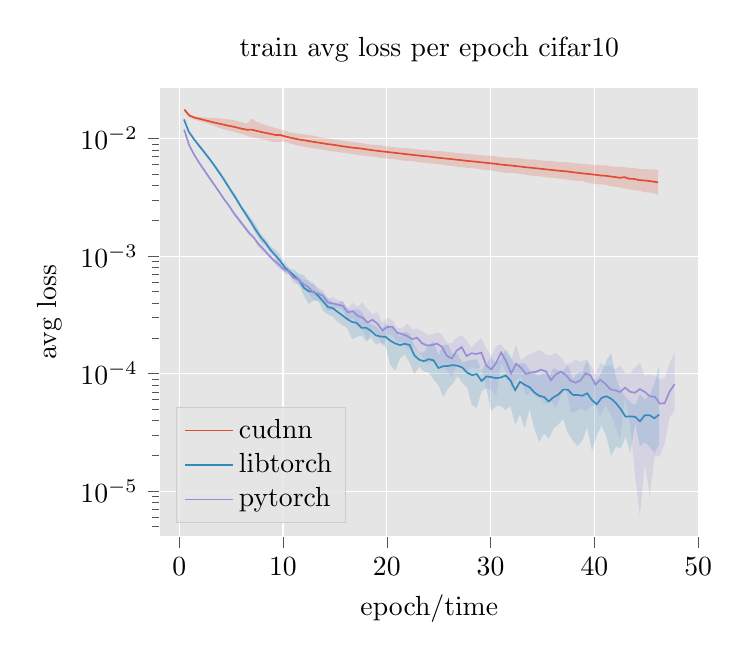
\begin{tikzpicture}

\definecolor{color0}{rgb}{0.886274509803922,0.290196078431373,0.2}
\definecolor{color1}{rgb}{0.203921568627451,0.541176470588235,0.741176470588235}
\definecolor{color2}{rgb}{0.596078431372549,0.556862745098039,0.835294117647059}

\begin{axis}[
axis background/.style={fill=white!89.8039215686275!black},
axis line style={white},
legend cell align={left},
legend style={fill opacity=0.8, draw opacity=1, text opacity=1, at={(0.03,0.03)}, anchor=south west, draw=white!80!black, fill=white!89.8039215686275!black},
log basis y={10},
tick align=outside,
tick pos=left,
title={train avg loss per epoch cifar10},
x grid style={white},
xlabel={epoch/time},
xmajorgrids,
xmin=-1.900079335, xmax=50.092281635,
xtick style={color=white!33.3333333333333!black},
y grid style={white},
ylabel={avg loss},
ymajorgrids,
ymin=4.13758073032916e-06, ymax=0.026969960001511,
ymode=log,
ytick style={color=white!33.3333333333333!black}
]
\path [fill=color0, fill opacity=0.2, very thin]
(axis cs:0.5020421,0.018093)
--(axis cs:0.5020421,0.016886)
--(axis cs:0.963857,0.015153)
--(axis cs:1.4278116,0.014544)
--(axis cs:1.887862,0.01411)
--(axis cs:2.3517187,0.013684)
--(axis cs:2.814011,0.013352)
--(axis cs:3.2743385,0.012922)
--(axis cs:3.7374035,0.012423)
--(axis cs:4.1995907,0.012067)
--(axis cs:4.6610242,0.011763)
--(axis cs:5.1238393,0.011513)
--(axis cs:5.585175,0.011132)
--(axis cs:6.0472547,0.010927)
--(axis cs:6.5086389,0.010603)
--(axis cs:6.9714158,0.010282)
--(axis cs:7.4346022,0.010091)
--(axis cs:7.8944034,0.009867)
--(axis cs:8.3578985,0.009718)
--(axis cs:8.8196617,0.009467)
--(axis cs:9.280207,0.009283)
--(axis cs:9.7445212,0.009392)
--(axis cs:10.20442,0.009389)
--(axis cs:10.6626901,0.009089)
--(axis cs:11.1237508,0.008864)
--(axis cs:11.5831099,0.008644)
--(axis cs:12.0413243,0.008528)
--(axis cs:12.5019929,0.008331)
--(axis cs:12.9604575,0.008246)
--(axis cs:13.419769,0.008143)
--(axis cs:13.8804618,0.008017)
--(axis cs:14.33941,0.007882)
--(axis cs:14.798587,0.00777)
--(axis cs:15.2587694,0.007679)
--(axis cs:15.7175274,0.007576)
--(axis cs:16.177363,0.007526)
--(axis cs:16.6381121,0.007367)
--(axis cs:17.0964306,0.007294)
--(axis cs:17.5551636,0.007184)
--(axis cs:18.0158013,0.007103)
--(axis cs:18.4753143,0.007042)
--(axis cs:18.9333992,0.00696)
--(axis cs:19.3940638,0.006849)
--(axis cs:19.855002,0.006795)
--(axis cs:20.3176195,0.006697)
--(axis cs:20.7764694,0.006662)
--(axis cs:21.2347057,0.006544)
--(axis cs:21.6951497,0.00646)
--(axis cs:22.1549523,0.006456)
--(axis cs:22.6133227,0.006383)
--(axis cs:23.072804,0.006283)
--(axis cs:23.5333105,0.006233)
--(axis cs:23.9920801,0.006169)
--(axis cs:24.4511959,0.006109)
--(axis cs:24.9115622,0.006057)
--(axis cs:25.3712205,0.005996)
--(axis cs:25.8296279,0.005885)
--(axis cs:26.2903579,0.005848)
--(axis cs:26.7499979,0.005766)
--(axis cs:27.2090298,0.005716)
--(axis cs:27.6685594,0.005635)
--(axis cs:28.1287852,0.005591)
--(axis cs:28.5873968,0.005569)
--(axis cs:29.0473541,0.005476)
--(axis cs:29.5077789,0.005395)
--(axis cs:29.9678529,0.005373)
--(axis cs:30.4307062,0.005289)
--(axis cs:30.8959481,0.005212)
--(axis cs:31.3575867,0.005113)
--(axis cs:31.8195534,0.005106)
--(axis cs:32.2810431,0.00508)
--(axis cs:32.7429998,0.005013)
--(axis cs:33.2052788,0.004946)
--(axis cs:33.6670195,0.004858)
--(axis cs:34.1293175,0.004815)
--(axis cs:34.591892,0.004777)
--(axis cs:35.0531397,0.004737)
--(axis cs:35.515564,0.004671)
--(axis cs:35.9772383,0.004629)
--(axis cs:36.4393094,0.004583)
--(axis cs:36.9014965,0.004525)
--(axis cs:37.3627614,0.00449)
--(axis cs:37.8255205,0.00441)
--(axis cs:38.2867267,0.004367)
--(axis cs:38.7492604,0.004361)
--(axis cs:39.210391,0.004239)
--(axis cs:39.6720935,0.004168)
--(axis cs:40.1342356,0.004088)
--(axis cs:40.5967315,0.004072)
--(axis cs:41.0580096,0.004057)
--(axis cs:41.5196336,0.003929)
--(axis cs:41.983765,0.003898)
--(axis cs:42.4478849,0.003838)
--(axis cs:42.9082525,0.003743)
--(axis cs:43.3715823,0.003706)
--(axis cs:43.8334075,0.003619)
--(axis cs:44.2975417,0.003611)
--(axis cs:44.7591353,0.003506)
--(axis cs:45.2199822,0.003473)
--(axis cs:45.6826783,0.003437)
--(axis cs:46.1443844,0.003301)
--(axis cs:46.1443844,0.005379)
--(axis cs:46.1443844,0.005379)
--(axis cs:45.6826783,0.005471)
--(axis cs:45.2199822,0.005477)
--(axis cs:44.7591353,0.005509)
--(axis cs:44.2975417,0.005498)
--(axis cs:43.8334075,0.00565)
--(axis cs:43.3715823,0.005615)
--(axis cs:42.9082525,0.005704)
--(axis cs:42.4478849,0.005752)
--(axis cs:41.983765,0.005772)
--(axis cs:41.5196336,0.005815)
--(axis cs:41.0580096,0.00593)
--(axis cs:40.5967315,0.005914)
--(axis cs:40.1342356,0.005974)
--(axis cs:39.6720935,0.006004)
--(axis cs:39.210391,0.006054)
--(axis cs:38.7492604,0.006103)
--(axis cs:38.2867267,0.006149)
--(axis cs:37.8255205,0.006215)
--(axis cs:37.3627614,0.006277)
--(axis cs:36.9014965,0.006291)
--(axis cs:36.4393094,0.006316)
--(axis cs:35.9772383,0.006455)
--(axis cs:35.515564,0.006429)
--(axis cs:35.0531397,0.006502)
--(axis cs:34.591892,0.006548)
--(axis cs:34.1293175,0.006657)
--(axis cs:33.6670195,0.006616)
--(axis cs:33.2052788,0.006727)
--(axis cs:32.7429998,0.006791)
--(axis cs:32.2810431,0.006839)
--(axis cs:31.8195534,0.006878)
--(axis cs:31.3575867,0.00692)
--(axis cs:30.8959481,0.00696)
--(axis cs:30.4307062,0.007077)
--(axis cs:29.9678529,0.007151)
--(axis cs:29.5077789,0.007155)
--(axis cs:29.0473541,0.007223)
--(axis cs:28.5873968,0.007273)
--(axis cs:28.1287852,0.007357)
--(axis cs:27.6685594,0.007414)
--(axis cs:27.2090298,0.007483)
--(axis cs:26.7499979,0.00753)
--(axis cs:26.2903579,0.007628)
--(axis cs:25.8296279,0.007707)
--(axis cs:25.3712205,0.007781)
--(axis cs:24.9115622,0.007838)
--(axis cs:24.4511959,0.007852)
--(axis cs:23.9920801,0.007945)
--(axis cs:23.5333105,0.008014)
--(axis cs:23.072804,0.008068)
--(axis cs:22.6133227,0.008166)
--(axis cs:22.1549523,0.008226)
--(axis cs:21.6951497,0.008323)
--(axis cs:21.2347057,0.008347)
--(axis cs:20.7764694,0.008423)
--(axis cs:20.3176195,0.008522)
--(axis cs:19.855002,0.008623)
--(axis cs:19.3940638,0.008786)
--(axis cs:18.9333992,0.008824)
--(axis cs:18.4753143,0.008883)
--(axis cs:18.0158013,0.008953)
--(axis cs:17.5551636,0.00916)
--(axis cs:17.0964306,0.009263)
--(axis cs:16.6381121,0.00938)
--(axis cs:16.177363,0.00946)
--(axis cs:15.7175274,0.00958)
--(axis cs:15.2587694,0.009729)
--(axis cs:14.798587,0.009891)
--(axis cs:14.33941,0.01001)
--(axis cs:13.8804618,0.010116)
--(axis cs:13.419769,0.010298)
--(axis cs:12.9604575,0.010568)
--(axis cs:12.5019929,0.010726)
--(axis cs:12.0413243,0.01087)
--(axis cs:11.5831099,0.010987)
--(axis cs:11.1237508,0.011097)
--(axis cs:10.6626901,0.011266)
--(axis cs:10.20442,0.011655)
--(axis cs:9.7445212,0.011937)
--(axis cs:9.280207,0.012308)
--(axis cs:8.8196617,0.012626)
--(axis cs:8.3578985,0.013013)
--(axis cs:7.8944034,0.013443)
--(axis cs:7.4346022,0.013932)
--(axis cs:6.9714158,0.014789)
--(axis cs:6.5086389,0.01338)
--(axis cs:6.0472547,0.013745)
--(axis cs:5.585175,0.014088)
--(axis cs:5.1238393,0.014433)
--(axis cs:4.6610242,0.014592)
--(axis cs:4.1995907,0.014738)
--(axis cs:3.7374035,0.014854)
--(axis cs:3.2743385,0.01497)
--(axis cs:2.814011,0.015078)
--(axis cs:2.3517187,0.015153)
--(axis cs:1.887862,0.015292)
--(axis cs:1.4278116,0.015451)
--(axis cs:0.963857,0.016212)
--(axis cs:0.5020421,0.018093)
--cycle;

\path [fill=color1, fill opacity=0.2, very thin]
(axis cs:0.4632098,0.014829)
--(axis cs:0.4632098,0.014249)
--(axis cs:0.9254774,0.011255)
--(axis cs:1.3881775,0.00979)
--(axis cs:1.8505787,0.008596)
--(axis cs:2.3129487,0.007637)
--(axis cs:2.7754109,0.006809)
--(axis cs:3.2376126,0.005988)
--(axis cs:3.6997682,0.005237)
--(axis cs:4.1622696,0.004525)
--(axis cs:4.6251273,0.003902)
--(axis cs:5.087667,0.003339)
--(axis cs:5.5501337,0.00287)
--(axis cs:6.0128713,0.002502)
--(axis cs:6.475329,0.002126)
--(axis cs:6.9379307,0.001817)
--(axis cs:7.4001751,0.001523)
--(axis cs:7.8623721,0.001314)
--(axis cs:8.3247837,0.001209)
--(axis cs:8.7869458,0.001054)
--(axis cs:9.2494491,0.000963)
--(axis cs:9.7118139,0.00081)
--(axis cs:10.1743406,0.000714)
--(axis cs:10.6367708,0.000692)
--(axis cs:11.0990792,0.000623)
--(axis cs:11.5616002,0.000563)
--(axis cs:12.023917,0.000456)
--(axis cs:12.4861342,0.000391)
--(axis cs:12.9482964,0.000421)
--(axis cs:13.4110369,0.000412)
--(axis cs:13.8734364,0.00034)
--(axis cs:14.3356181,0.000318)
--(axis cs:14.7980995,0.000306)
--(axis cs:15.2603591,0.000275)
--(axis cs:15.7226721,0.000258)
--(axis cs:16.1851398,0.000244)
--(axis cs:16.6474628,0.000197)
--(axis cs:17.109834,0.000205)
--(axis cs:17.5721993,0.000211)
--(axis cs:18.0343757,0.000187)
--(axis cs:18.4972186,0.000202)
--(axis cs:18.9595973,0.000176)
--(axis cs:19.4217701,0.000184)
--(axis cs:19.8841996,0.000171)
--(axis cs:20.3465831,0.000118)
--(axis cs:20.808959,0.000106)
--(axis cs:21.2711594,0.000135)
--(axis cs:21.7335873,0.000145)
--(axis cs:22.1956461,0.000124)
--(axis cs:22.6579044,9.9e-05)
--(axis cs:23.1202674,0.000114)
--(axis cs:23.5825376,0.000104)
--(axis cs:24.0448372,0.000102)
--(axis cs:24.5074876,8.9e-05)
--(axis cs:24.9699805,8e-05)
--(axis cs:25.4322128,6.3e-05)
--(axis cs:25.8946321,7.4e-05)
--(axis cs:26.3568754,8.2e-05)
--(axis cs:26.8195408,9.5e-05)
--(axis cs:27.2818438,8.3e-05)
--(axis cs:27.7444919,7.6e-05)
--(axis cs:28.2070578,5.4e-05)
--(axis cs:28.6696802,5.1e-05)
--(axis cs:29.1318423,7.1e-05)
--(axis cs:29.594161,7.5e-05)
--(axis cs:30.0567959,4.8e-05)
--(axis cs:30.5192224,5.3e-05)
--(axis cs:30.9818398,5.3e-05)
--(axis cs:31.4445083,4.9e-05)
--(axis cs:31.9071473,5.3e-05)
--(axis cs:32.3696306,3.7e-05)
--(axis cs:32.8321084,4.5e-05)
--(axis cs:33.2945942,3.4e-05)
--(axis cs:33.757296,5e-05)
--(axis cs:34.2195982,3.4e-05)
--(axis cs:34.6819453,2.6e-05)
--(axis cs:35.144328,3.1e-05)
--(axis cs:35.6066388,2.8e-05)
--(axis cs:36.0693839,3.4e-05)
--(axis cs:36.5320704,3.7e-05)
--(axis cs:36.9945851,4.1e-05)
--(axis cs:37.4569107,3.1e-05)
--(axis cs:37.9197657,2.7e-05)
--(axis cs:38.3823447,2.4e-05)
--(axis cs:38.844871,2.7e-05)
--(axis cs:39.3072444,3.5e-05)
--(axis cs:39.7696805,2.2e-05)
--(axis cs:40.2319381,3e-05)
--(axis cs:40.6940758,3.6e-05)
--(axis cs:41.1565834,2.9e-05)
--(axis cs:41.6190216,2e-05)
--(axis cs:42.0813775,2.4e-05)
--(axis cs:42.5436282,2.3e-05)
--(axis cs:43.0058633,2.9e-05)
--(axis cs:43.4683882,2.1e-05)
--(axis cs:43.930484,3.8e-05)
--(axis cs:44.3925875,2.4e-05)
--(axis cs:44.8548618,2.6e-05)
--(axis cs:45.3173953,2.4e-05)
--(axis cs:45.7795459,2.1e-05)
--(axis cs:46.2420028,2.5e-05)
--(axis cs:46.2420028,0.000117)
--(axis cs:46.2420028,0.000117)
--(axis cs:45.7795459,8.2e-05)
--(axis cs:45.3173953,6.5e-05)
--(axis cs:44.8548618,6e-05)
--(axis cs:44.3925875,6.7e-05)
--(axis cs:43.930484,5.4e-05)
--(axis cs:43.4683882,5.7e-05)
--(axis cs:43.0058633,6.3e-05)
--(axis cs:42.5436282,7.2e-05)
--(axis cs:42.0813775,9.2e-05)
--(axis cs:41.6190216,0.000149)
--(axis cs:41.1565834,0.00013)
--(axis cs:40.6940758,0.000101)
--(axis cs:40.2319381,8.9e-05)
--(axis cs:39.7696805,9.1e-05)
--(axis cs:39.3072444,0.000133)
--(axis cs:38.844871,0.000103)
--(axis cs:38.3823447,0.000101)
--(axis cs:37.9197657,9e-05)
--(axis cs:37.4569107,0.000119)
--(axis cs:36.9945851,0.000105)
--(axis cs:36.5320704,0.000106)
--(axis cs:36.0693839,0.000112)
--(axis cs:35.6066388,9.3e-05)
--(axis cs:35.144328,0.000101)
--(axis cs:34.6819453,9.6e-05)
--(axis cs:34.2195982,0.0001)
--(axis cs:33.757296,0.000108)
--(axis cs:33.2945942,0.000122)
--(axis cs:32.8321084,0.000122)
--(axis cs:32.3696306,0.000116)
--(axis cs:31.9071473,0.000142)
--(axis cs:31.4445083,0.000162)
--(axis cs:30.9818398,0.000132)
--(axis cs:30.5192224,0.000123)
--(axis cs:30.0567959,0.000137)
--(axis cs:29.594161,0.000122)
--(axis cs:29.1318423,0.000108)
--(axis cs:28.6696802,0.000133)
--(axis cs:28.2070578,0.00013)
--(axis cs:27.7444919,0.000129)
--(axis cs:27.2818438,0.000125)
--(axis cs:26.8195408,0.000148)
--(axis cs:26.3568754,0.000146)
--(axis cs:25.8946321,0.000176)
--(axis cs:25.4322128,0.000174)
--(axis cs:24.9699805,0.000143)
--(axis cs:24.5074876,0.000189)
--(axis cs:24.0448372,0.000174)
--(axis cs:23.5825376,0.000152)
--(axis cs:23.1202674,0.00015)
--(axis cs:22.6579044,0.000173)
--(axis cs:22.1956461,0.000219)
--(axis cs:21.7335873,0.000228)
--(axis cs:21.2711594,0.000208)
--(axis cs:20.808959,0.000225)
--(axis cs:20.3465831,0.000254)
--(axis cs:19.8841996,0.000265)
--(axis cs:19.4217701,0.000227)
--(axis cs:18.9595973,0.000252)
--(axis cs:18.4972186,0.000263)
--(axis cs:18.0343757,0.000284)
--(axis cs:17.5721993,0.000335)
--(axis cs:17.109834,0.000359)
--(axis cs:16.6474628,0.000336)
--(axis cs:16.1851398,0.000362)
--(axis cs:15.7226721,0.000417)
--(axis cs:15.2603591,0.000397)
--(axis cs:14.7980995,0.000405)
--(axis cs:14.3356181,0.000435)
--(axis cs:13.8734364,0.000483)
--(axis cs:13.4110369,0.000515)
--(axis cs:12.9482964,0.000575)
--(axis cs:12.4861342,0.0006)
--(axis cs:12.023917,0.000688)
--(axis cs:11.5616002,0.000704)
--(axis cs:11.0990792,0.000762)
--(axis cs:10.6367708,0.000785)
--(axis cs:10.1743406,0.000888)
--(axis cs:9.7118139,0.001031)
--(axis cs:9.2494491,0.001136)
--(axis cs:8.7869458,0.001214)
--(axis cs:8.3247837,0.001397)
--(axis cs:7.8623721,0.001548)
--(axis cs:7.4001751,0.001839)
--(axis cs:6.9379307,0.002105)
--(axis cs:6.475329,0.00239)
--(axis cs:6.0128713,0.00269)
--(axis cs:5.5501337,0.003209)
--(axis cs:5.087667,0.00364)
--(axis cs:4.6251273,0.004256)
--(axis cs:4.1622696,0.004922)
--(axis cs:3.6997682,0.005622)
--(axis cs:3.2376126,0.006421)
--(axis cs:2.7754109,0.007228)
--(axis cs:2.3129487,0.008191)
--(axis cs:1.8505787,0.009114)
--(axis cs:1.3881775,0.010215)
--(axis cs:0.9254774,0.011713)
--(axis cs:0.4632098,0.014829)
--cycle;

\path [fill=color2, fill opacity=0.2, very thin]
(axis cs:0.4787409,0.0120750022)
--(axis cs:0.4787409,0.0117503989)
--(axis cs:0.9549568,0.00865785)
--(axis cs:1.4328986,0.0071526477)
--(axis cs:1.9128344,0.006115615)
--(axis cs:2.3927933,0.0052511538)
--(axis cs:2.875019,0.0045624886)
--(axis cs:3.3514207,0.0040074299)
--(axis cs:3.8258368,0.0034686722)
--(axis cs:4.3021816,0.0029761007)
--(axis cs:4.7785431,0.0025864496)
--(axis cs:5.2544502,0.0022351847)
--(axis cs:5.7327906,0.0019379215)
--(axis cs:6.2106256,0.0017476827)
--(axis cs:6.6934447,0.0015134937)
--(axis cs:7.1764946,0.0013892412)
--(axis cs:7.6527392,0.0011825239)
--(axis cs:8.1276748,0.0010753832)
--(axis cs:8.6052351,0.0009816324)
--(axis cs:9.0833687,0.0008862796)
--(axis cs:9.5603715,0.0007888771)
--(axis cs:10.0355231,0.0007387705)
--(axis cs:10.5112275,0.0007037375)
--(axis cs:10.9890443,0.0005910762)
--(axis cs:11.4700498,0.0005731388)
--(axis cs:11.9460153,0.0005363433)
--(axis cs:12.4240194,0.0004885938)
--(axis cs:12.9025472,0.0004232642)
--(axis cs:13.3790138,0.0004175752)
--(axis cs:13.8546063,0.0004028942)
--(axis cs:14.3295909,0.0003381217)
--(axis cs:14.8081463,0.0003508446)
--(axis cs:15.289785,0.0003668604)
--(axis cs:15.7659315,0.0003473249)
--(axis cs:16.2408114,0.0002907149)
--(axis cs:16.7177102,0.0002959099)
--(axis cs:17.1941908,0.0002494935)
--(axis cs:17.6725458,0.0002349354)
--(axis cs:18.153403,0.0001934963)
--(axis cs:18.631386,0.0002453622)
--(axis cs:19.1072212,0.0002138886)
--(axis cs:19.5814395,0.0001694002)
--(axis cs:20.0587741,0.0002149288)
--(axis cs:20.5357722,0.0002143415)
--(axis cs:21.0118284,0.0001839784)
--(axis cs:21.4875376,0.0001847615)
--(axis cs:21.9662875,0.0001622335)
--(axis cs:22.4450026,0.0001709925)
--(axis cs:22.921241,0.0001571253)
--(axis cs:23.3970977,0.0001414303)
--(axis cs:23.8751955,0.0001207844)
--(axis cs:24.3509275,0.0001265899)
--(axis cs:24.8275496,0.0001185389)
--(axis cs:25.3055867,0.0001137668)
--(axis cs:25.784609,0.0001060493)
--(axis cs:26.26137,9.29983e-05)
--(axis cs:26.7373334,0.0001188804)
--(axis cs:27.2131395,0.0001112901)
--(axis cs:27.6884838,0.0001022692)
--(axis cs:28.1644315,0.0001143315)
--(axis cs:28.6431342,0.0001097178)
--(axis cs:29.1211952,0.0001148819)
--(axis cs:29.597205,7.5027e-05)
--(axis cs:30.074211,7.262e-05)
--(axis cs:30.5499029,6.49622e-05)
--(axis cs:31.0274016,0.0001242268)
--(axis cs:31.5027262,0.0001031197)
--(axis cs:31.9795899,7.56704e-05)
--(axis cs:32.4580046,8.79002e-05)
--(axis cs:32.9333126,9.32847e-05)
--(axis cs:33.4104359,6.47454e-05)
--(axis cs:33.8869678,7.1128e-05)
--(axis cs:34.3650765,6.43873e-05)
--(axis cs:34.8432337,6.12894e-05)
--(axis cs:35.3232167,5.49014e-05)
--(axis cs:35.8059391,5.91588e-05)
--(axis cs:36.2872295,5.05937e-05)
--(axis cs:36.763833,6.40597e-05)
--(axis cs:37.2396782,7.64006e-05)
--(axis cs:37.7172186,4.65381e-05)
--(axis cs:38.1930911,4.70601e-05)
--(axis cs:38.6720442,5.03463e-05)
--(axis cs:39.1488671,4.77045e-05)
--(axis cs:39.6243587,5.19172e-05)
--(axis cs:40.0995631,5.45186e-05)
--(axis cs:40.5750744,4.34181e-05)
--(axis cs:41.0521059,5.36213e-05)
--(axis cs:41.5299999,4.60973e-05)
--(axis cs:42.0052569,3.60851e-05)
--(axis cs:42.4803443,2.75153e-05)
--(axis cs:42.9563098,6.31907e-05)
--(axis cs:43.4326693,3.7695e-05)
--(axis cs:43.9082268,1.39669e-05)
--(axis cs:44.3837151,6.1676e-06)
--(axis cs:44.8605593,1.66676e-05)
--(axis cs:45.340364,9.1898e-06)
--(axis cs:45.8189316,1.97946e-05)
--(axis cs:46.296049,1.97743e-05)
--(axis cs:46.7714856,2.5465e-05)
--(axis cs:47.2480983,4.2502e-05)
--(axis cs:47.7289925,4.84777e-05)
--(axis cs:47.7289925,0.0001519406)
--(axis cs:47.7289925,0.0001519406)
--(axis cs:47.2480983,0.0001213709)
--(axis cs:46.7714856,9.18354e-05)
--(axis cs:46.296049,8.93854e-05)
--(axis cs:45.8189316,9.59958e-05)
--(axis cs:45.340364,9.76159e-05)
--(axis cs:44.8605593,9.53637e-05)
--(axis cs:44.3837151,0.0001233603)
--(axis cs:43.9082268,0.0001129035)
--(axis cs:43.4326693,0.000100086)
--(axis cs:42.9563098,0.0001010479)
--(axis cs:42.4803443,0.0001178649)
--(axis cs:42.0052569,0.0001088219)
--(axis cs:41.5299999,0.0001183068)
--(axis cs:41.0521059,0.0001150748)
--(axis cs:40.5750744,0.0001234193)
--(axis cs:40.0995631,9.72259e-05)
--(axis cs:39.6243587,0.0001192488)
--(axis cs:39.1488671,0.0001316667)
--(axis cs:38.6720442,0.0001259231)
--(axis cs:38.1930911,0.0001314788)
--(axis cs:37.7172186,0.0001230752)
--(axis cs:37.2396782,0.000119555)
--(axis cs:36.763833,0.0001386038)
--(axis cs:36.2872295,0.0001503085)
--(axis cs:35.8059391,0.0001426814)
--(axis cs:35.3232167,0.0001442273)
--(axis cs:34.8432337,0.0001577955)
--(axis cs:34.3650765,0.0001551934)
--(axis cs:33.8869678,0.0001465462)
--(axis cs:33.4104359,0.0001416965)
--(axis cs:32.9333126,0.0001284432)
--(axis cs:32.4580046,0.0001781978)
--(axis cs:31.9795899,0.0001299068)
--(axis cs:31.5027262,0.0001502897)
--(axis cs:31.0274016,0.0001782036)
--(axis cs:30.5499029,0.0001724946)
--(axis cs:30.074211,0.0001419183)
--(axis cs:29.597205,0.0001622314)
--(axis cs:29.1211952,0.0002003582)
--(axis cs:28.6431342,0.000185485)
--(axis cs:28.1644315,0.0001664169)
--(axis cs:27.6884838,0.0001914532)
--(axis cs:27.2131395,0.0002123293)
--(axis cs:26.7373334,0.000203174)
--(axis cs:26.26137,0.0001810373)
--(axis cs:25.784609,0.00018181)
--(axis cs:25.3055867,0.00021596)
--(axis cs:24.8275496,0.0002245644)
--(axis cs:24.3509275,0.0002152208)
--(axis cs:23.8751955,0.0002151001)
--(axis cs:23.3970977,0.0002299341)
--(axis cs:22.921241,0.0002429364)
--(axis cs:22.4450026,0.0002371008)
--(axis cs:21.9662875,0.0002673427)
--(axis cs:21.4875376,0.0002418086)
--(axis cs:21.0118284,0.0002436904)
--(axis cs:20.5357722,0.0002866595)
--(axis cs:20.0587741,0.0002994981)
--(axis cs:19.5814395,0.0002694565)
--(axis cs:19.1072212,0.000333757)
--(axis cs:18.631386,0.0003209846)
--(axis cs:18.153403,0.0003524054)
--(axis cs:17.6725458,0.0004042682)
--(axis cs:17.1941908,0.0003684314)
--(axis cs:16.7177102,0.0004010363)
--(axis cs:16.2408114,0.0003550824)
--(axis cs:15.7659315,0.0004135631)
--(axis cs:15.289785,0.000419638)
--(axis cs:14.8081463,0.0004510758)
--(axis cs:14.3295909,0.000435752)
--(axis cs:13.8546063,0.0005127314)
--(axis cs:13.3790138,0.0005383109)
--(axis cs:12.9025472,0.0005949302)
--(axis cs:12.4240194,0.0006295708)
--(axis cs:11.9460153,0.0006247492)
--(axis cs:11.4700498,0.000687465)
--(axis cs:10.9890443,0.0007125788)
--(axis cs:10.5112275,0.0007870662)
--(axis cs:10.0355231,0.0008201759)
--(axis cs:9.5603715,0.0009233276)
--(axis cs:9.0833687,0.0009451787)
--(axis cs:8.6052351,0.0010609791)
--(axis cs:8.1276748,0.001209327)
--(axis cs:7.6527392,0.0013049251)
--(axis cs:7.1764946,0.0015021397)
--(axis cs:6.6934447,0.0016780356)
--(axis cs:6.2106256,0.0018762267)
--(axis cs:5.7327906,0.002119968)
--(axis cs:5.2544502,0.0024070138)
--(axis cs:4.7785431,0.0027729336)
--(axis cs:4.3021816,0.0031334486)
--(axis cs:3.8258368,0.0036234653)
--(axis cs:3.3514207,0.0041529231)
--(axis cs:2.875019,0.0047467432)
--(axis cs:2.3927933,0.0054820664)
--(axis cs:1.9128344,0.0063237132)
--(axis cs:1.4328986,0.0073941951)
--(axis cs:0.9549568,0.0089143509)
--(axis cs:0.4787409,0.0120750022)
--cycle;

\addplot [semithick, color0]
table {%
0.502042055130005 0.0176223311573267
0.963856935501099 0.0157266017049551
1.42781162261963 0.0151215996593237
3.27433848381042 0.0137485014274716
4.66102409362793 0.012899300083518
5.12383937835693 0.0126724010333419
6.04725456237793 0.0121083995327353
6.50863885879517 0.0118798995390534
6.97141599655151 0.0119089996442199
7.8944034576416 0.0113715985789895
9.28020668029785 0.0107231987640262
9.74452114105225 0.0107188988476992
10.2044200897217 0.0104198986664414
11.1237506866455 0.0099835991859436
11.5831098556519 0.00980240292847157
12.0413246154785 0.00967140030115843
12.5019931793213 0.00950410030782223
13.8804616928101 0.0090930974110961
14.339409828186 0.00895489938557148
14.7985868453979 0.00886359997093678
15.7175273895264 0.00859829783439636
16.6381130218506 0.00837740115821362
17.0964298248291 0.00830739922821522
18.9333992004395 0.00789029989391565
23.5333099365234 0.00708530005067587
23.9920806884766 0.00703849922865629
24.9115619659424 0.00686590187251568
27.2090301513672 0.00654359860345721
27.6685600280762 0.00645839888602495
28.1287860870361 0.00641159806400537
29.9678535461426 0.00616110069677234
30.4307060241699 0.00610629888251424
30.8959484100342 0.0060197995044291
31.3575859069824 0.00595740089192986
31.8195533752441 0.00591539964079857
33.2052803039551 0.00572519889101386
36.901496887207 0.00528909964486957
37.3627624511719 0.00525570102035999
37.8255195617676 0.00517309969291091
40.1342353820801 0.00491449842229486
40.5967330932617 0.00484839919954538
41.0580101013184 0.00482469936832786
42.447883605957 0.00463760085403919
42.9082527160645 0.00469200126826763
43.37158203125 0.00454699900001287
43.8334083557129 0.00452959863469005
44.2975425720215 0.00443029962480068
44.7591361999512 0.00440330058336258
45.6826782226562 0.00430449843406677
46.1443862915039 0.00422980030998588
};
\addlegendentry{cudnn}
\addplot [semithick, color1]
table {%
0.463209867477417 0.0145087987184525
0.925477385520935 0.0114285005256534
1.38817751407623 0.00997430272400379
1.85057866573334 0.00882810074836016
2.31294870376587 0.00786020141094923
2.77541089057922 0.00696539971977472
3.23761248588562 0.00614969944581389
4.16226959228516 0.00468830112367868
5.55013370513916 0.00301239965483546
6.01287126541138 0.00257330061867833
6.47532892227173 0.00223459978587925
6.93793058395386 0.00193249981384724
7.40017509460449 0.00165540038142353
7.86237192153931 0.00144380005076528
8.32478332519531 0.00129140017088503
8.78694534301758 0.0011324001243338
9.71181392669678 0.000915599812287837
10.1743402481079 0.000800399808213115
10.6367712020874 0.000737899797968566
11.5615997314453 0.000621999963186681
12.0239171981812 0.000535900006070733
12.4861345291138 0.000501400034409016
12.948296546936 0.000497300119604915
13.411036491394 0.000457299873232841
14.335618019104 0.000368400069419295
14.7980995178223 0.00036020009429194
15.2603588104248 0.000334999902406707
15.7226724624634 0.000313099910272285
16.1851406097412 0.000291399948764592
16.6474628448486 0.000275199970928952
17.1098346710205 0.00026959998649545
17.5721988677979 0.000244899973040447
18.0343761444092 0.000244799972278997
18.4972190856934 0.000230400037253276
18.9595966339111 0.000211299964576028
19.4217700958252 0.00020670001686085
19.8841991424561 0.000205599993932992
20.3465824127197 0.00019029997929465
20.8089580535889 0.000180599978193641
21.2711601257324 0.000174800050444901
21.7335872650146 0.000179500042577274
22.1956462860107 0.000175299952388741
22.6579036712646 0.000142899982165545
23.120267868042 0.000131199980387464
23.5825366973877 0.000127600011182949
24.0448379516602 0.000132700006361119
24.5074882507324 0.000129700027173385
24.9699802398682 0.000111599991214462
25.4322128295898 0.000115599978016689
25.8946323394775 0.000116199982585385
26.3568744659424 0.000118200012366287
26.8195400238037 0.000116600000183098
27.2818431854248 0.00011249998351559
27.7444915771484 0.000101699981314596
28.2070579528809 9.710002632346e-05
28.6696796417236 9.89999607554637e-05
29.1318416595459 8.65999536472373e-05
29.5941600799561 9.45999927353114e-05
30.0567951202393 9.35000498429872e-05
30.5192222595215 9.14999836822972e-05
30.981840133667 9.25999847822823e-05
31.444507598877 9.64999562711455e-05
31.9071464538574 8.76999547472224e-05
32.36962890625 7.230003393488e-05
32.8321075439453 8.53000383358449e-05
33.2945938110352 8.01999922259711e-05
33.7572975158691 7.66999655752443e-05
34.219596862793 6.9099995016586e-05
34.6819458007812 6.4799991378095e-05
35.1443290710449 6.32999726803973e-05
35.6066398620605 5.80000305490103e-05
36.0693855285645 6.30000286037102e-05
36.5320701599121 6.63999671814963e-05
36.9945869445801 7.30999963707291e-05
37.4569091796875 7.29999810573645e-05
37.9197654724121 6.58999852021225e-05
38.3823432922363 6.57999917166308e-05
38.8448715209961 6.49000285193324e-05
39.307243347168 6.80000230204314e-05
39.7696800231934 5.94000121054705e-05
40.2319374084473 5.4900021495996e-05
40.6940765380859 6.21000217506662e-05
41.1565818786621 6.4200023189187e-05
41.6190223693848 6.11999785178341e-05
42.0813789367676 5.61000015295576e-05
42.543628692627 4.98000044899527e-05
43.0058631896973 4.30000181950163e-05
43.4683876037598 4.33000059274491e-05
43.9304847717285 4.28999956056941e-05
44.3925857543945 3.93000191252213e-05
44.8548622131348 4.42000200564507e-05
45.3173942565918 4.43000062659848e-05
45.7795448303223 4.17000192101113e-05
46.2420043945312 4.47999991592951e-05
};
\addlegendentry{libtorch}
\addplot [semithick, color2]
table {%
0.478740930557251 0.0118992431089282
0.954956769943237 0.00878745131194592
1.43289864063263 0.00731339538469911
1.91283440589905 0.00624285126104951
2.87501907348633 0.00468650227412581
3.82583689689636 0.00354621536098421
4.30218172073364 0.00306860567070544
4.77854299545288 0.00269876886159182
5.25445032119751 0.00232950202189386
6.69344472885132 0.00158972875215113
7.17649459838867 0.00143970479257405
7.65273904800415 0.00126123626250774
8.12767505645752 0.00114091578871012
8.60523509979248 0.00102516985498369
9.0833683013916 0.000926833890844136
9.56037139892578 0.000851463933940977
10.0355234146118 0.000776868895627558
10.5112276077271 0.000743681972380728
10.9890441894531 0.000653432973194867
11.4700498580933 0.000633495103102177
11.9460153579712 0.000578892009798437
12.4240198135376 0.000546346302144229
12.9025468826294 0.00049202295485884
13.3790140151978 0.000479624955914915
13.854606628418 0.00045882147969678
14.3295907974243 0.000402535137254745
14.8081464767456 0.000395345239667222
15.2897853851318 0.000385501596610993
15.7659311294556 0.000377818854758516
16.2408123016357 0.000331610994180664
16.7177104949951 0.000340495345881209
17.1941909790039 0.00031075460719876
17.6725463867188 0.000298347324132919
18.1534023284912 0.000272694625891745
18.6313858032227 0.0002868787269108
19.1072216033936 0.000265621521975845
19.5814399719238 0.000232754478929564
20.0587749481201 0.0002492651110515
20.5357723236084 0.000250101526034996
21.0118274688721 0.00022227356384974
21.4875373840332 0.000216823114897124
21.966287612915 0.000208507684874348
22.4450035095215 0.000196910492377356
22.9212417602539 0.000201836228370667
23.3970985412598 0.000181669442099519
23.8751945495605 0.000173442604136653
24.3509273529053 0.00017522789130453
24.8275489807129 0.000179912618477829
25.3055858612061 0.000168993210536428
25.7846088409424 0.000141701311804354
26.2613697052002 0.000134392583277076
26.7373332977295 0.00015690723375883
27.2131385803223 0.000168063590535894
27.6884841918945 0.000141158438054845
28.1644306182861 0.000148915205500089
28.6431350708008 0.000146946767927147
29.1211948394775 0.000150810141349211
29.597204208374 0.000116782830446027
30.0742111206055 0.000108423657366075
30.5499019622803 0.000124202008009888
31.027400970459 0.000150915002450347
31.5027256011963 0.000127319552120753
31.9795894622803 0.000100344746897463
32.4580039978027 0.000121575620141812
32.9333114624023 0.000111950183054432
33.4104347229004 9.92221757769585e-05
33.8869667053223 0.00010218373790849
34.3650779724121 0.000103525097074453
34.8432350158691 0.000107996005681343
35.3232154846191 0.000104844628367573
35.8059387207031 8.78753780853003e-05
36.2872276306152 9.86761369858868e-05
36.7638320922852 0.000104004793683998
37.2396774291992 9.73225614870898e-05
37.7172203063965 8.69100986164995e-05
38.1930923461914 8.37819679873064e-05
38.6720428466797 8.77572674653493e-05
39.148868560791 0.00010023017966887
39.6243591308594 9.66972293099388e-05
40.0995635986328 8.0752324720379e-05
40.5750732421875 8.84969922481105e-05
41.0521049499512 8.2011116319336e-05
41.5299987792969 7.36182191758417e-05
42.005256652832 7.20261305104941e-05
42.4803428649902 6.98780568200164e-05
42.9563102722168 7.59818140068091e-05
43.4326705932617 7.00582750141621e-05
43.9082260131836 6.88012660248205e-05
44.383716583252 7.379812450381e-05
44.8605575561523 6.98277435731143e-05
45.3403625488281 6.40918442513794e-05
45.8189315795898 6.36608747299761e-05
46.2960472106934 5.56393206352368e-05
46.771484375 5.60346270503942e-05
47.2480964660645 7.03939949744381e-05
47.7289924621582 8.1223071902059e-05
};
\addlegendentry{pytorch}
\end{axis}

\end{tikzpicture}

    \end{figure}


    \begin{figure}
        % This file was created by tikzplotlib v0.9.5.
\begin{tikzpicture}





\begin{axis}[
axis background/.style={fill=white!89.8039215686275!black},
axis line style={white},
legend cell align={left},
legend style={fill opacity=0.8, draw opacity=1, text opacity=1, at={(0.03,0.03)}, anchor=south west, draw=white!80!black, fill=white!89.8039215686275!black},
log basis y={10},
tick align=outside,
tick pos=left,
title={train avg loss per epoch stl10},
x grid style={white},
xlabel={epoch/time},
xmajorgrids,
xmin=-5.19760163, xmax=135.38068523,
xtick style={color=white!33.3333333333333!black},
y grid style={white},
ylabel={avg loss},
ymajorgrids,
ymin=1.12370019055739e-05, ymax=0.0267288376849893,
ymode=log,
ytick style={color=white!33.3333333333333!black}
]
\path [fill=cudnn, fill opacity=0.2, very thin]
(axis cs:3.1015922,0.018772)
--(axis cs:3.1015922,0.017531)
--(axis cs:4.3881964,0.016275)
--(axis cs:5.6697498,0.015518)
--(axis cs:6.9567745,0.015175)
--(axis cs:8.2428672,0.014871)
--(axis cs:9.5269492,0.014374)
--(axis cs:10.8122282,0.014222)
--(axis cs:12.0991791,0.013803)
--(axis cs:13.3812914,0.013697)
--(axis cs:14.6654891,0.013389)
--(axis cs:15.9478969,0.013263)
--(axis cs:17.232328,0.013074)
--(axis cs:18.5146575,0.013034)
--(axis cs:19.8012213,0.012883)
--(axis cs:21.0840842,0.012693)
--(axis cs:22.3683458,0.012653)
--(axis cs:23.651952,0.012548)
--(axis cs:24.9376781,0.012475)
--(axis cs:26.2201795,0.012382)
--(axis cs:27.5038189,0.012361)
--(axis cs:28.7885163,0.01221)
--(axis cs:30.0761489,0.012263)
--(axis cs:31.358376,0.012122)
--(axis cs:32.6423435,0.011945)
--(axis cs:33.9274175,0.012002)
--(axis cs:35.2126796,0.011843)
--(axis cs:36.4976855,0.011819)
--(axis cs:37.7835537,0.011759)
--(axis cs:39.0670015,0.011642)
--(axis cs:40.3503277,0.011648)
--(axis cs:41.6357876,0.011649)
--(axis cs:42.9215691,0.011474)
--(axis cs:44.2048227,0.01154)
--(axis cs:45.490117,0.011452)
--(axis cs:46.7742425,0.011321)
--(axis cs:48.0608687,0.011262)
--(axis cs:49.3439484,0.011238)
--(axis cs:50.628987,0.011274)
--(axis cs:51.9142668,0.011119)
--(axis cs:53.1983139,0.011047)
--(axis cs:54.4834733,0.011049)
--(axis cs:55.7678699,0.011029)
--(axis cs:57.0510268,0.011095)
--(axis cs:58.3349453,0.010864)
--(axis cs:59.6192652,0.010941)
--(axis cs:60.9042402,0.01088)
--(axis cs:62.1854784,0.010752)
--(axis cs:63.4683535,0.010674)
--(axis cs:64.7523611,0.010699)
--(axis cs:66.0399125,0.010662)
--(axis cs:67.3233237,0.010667)
--(axis cs:68.6089274,0.01053)
--(axis cs:69.8913879,0.010445)
--(axis cs:71.1745869,0.010516)
--(axis cs:72.4576266,0.010424)
--(axis cs:73.7439566,0.010317)
--(axis cs:75.0281581,0.010287)
--(axis cs:76.3165164,0.010292)
--(axis cs:77.5979577,0.010204)
--(axis cs:78.8851048,0.010214)
--(axis cs:80.1680884,0.010135)
--(axis cs:81.4541719,0.010121)
--(axis cs:82.738797,0.010027)
--(axis cs:84.0242694,0.010073)
--(axis cs:85.3116352,0.010059)
--(axis cs:86.5965253,0.010086)
--(axis cs:87.8830559,0.009988)
--(axis cs:89.1684826,0.009911)
--(axis cs:90.451034,0.009908)
--(axis cs:91.7357714,0.009823)
--(axis cs:93.0172198,0.009768)
--(axis cs:94.3033933,0.009768)
--(axis cs:95.5860217,0.009777)
--(axis cs:96.8740081,0.009605)
--(axis cs:98.1589983,0.009755)
--(axis cs:99.4438364,0.00958)
--(axis cs:100.726415,0.009649)
--(axis cs:102.009401,0.009472)
--(axis cs:103.2938186,0.009554)
--(axis cs:104.5794376,0.009464)
--(axis cs:105.8616588,0.009402)
--(axis cs:107.1464607,0.009436)
--(axis cs:108.4291424,0.009381)
--(axis cs:109.7167975,0.009291)
--(axis cs:111.0016509,0.009343)
--(axis cs:112.2889483,0.00928)
--(axis cs:113.5706432,0.00921)
--(axis cs:114.855097,0.009163)
--(axis cs:116.1407626,0.009147)
--(axis cs:117.4265288,0.009166)
--(axis cs:118.7118835,0.009017)
--(axis cs:119.9955895,0.009014)
--(axis cs:121.2795428,0.008957)
--(axis cs:122.567516,0.008943)
--(axis cs:123.8486356,0.008985)
--(axis cs:125.1355257,0.008861)
--(axis cs:126.4196376,0.008766)
--(axis cs:127.7084405,0.008834)
--(axis cs:128.9907631,0.008816)
--(axis cs:128.9907631,0.01134)
--(axis cs:128.9907631,0.01134)
--(axis cs:127.7084405,0.01121)
--(axis cs:126.4196376,0.011294)
--(axis cs:125.1355257,0.011317)
--(axis cs:123.8486356,0.011356)
--(axis cs:122.567516,0.011347)
--(axis cs:121.2795428,0.011333)
--(axis cs:119.9955895,0.011389)
--(axis cs:118.7118835,0.011417)
--(axis cs:117.4265288,0.011411)
--(axis cs:116.1407626,0.011458)
--(axis cs:114.855097,0.01149)
--(axis cs:113.5706432,0.011471)
--(axis cs:112.2889483,0.01152)
--(axis cs:111.0016509,0.01156)
--(axis cs:109.7167975,0.011554)
--(axis cs:108.4291424,0.011577)
--(axis cs:107.1464607,0.011593)
--(axis cs:105.8616588,0.011632)
--(axis cs:104.5794376,0.011723)
--(axis cs:103.2938186,0.011685)
--(axis cs:102.009401,0.011753)
--(axis cs:100.726415,0.01176)
--(axis cs:99.4438364,0.011837)
--(axis cs:98.1589983,0.011812)
--(axis cs:96.8740081,0.011833)
--(axis cs:95.5860217,0.011902)
--(axis cs:94.3033933,0.011932)
--(axis cs:93.0172198,0.011904)
--(axis cs:91.7357714,0.011963)
--(axis cs:90.451034,0.011958)
--(axis cs:89.1684826,0.012088)
--(axis cs:87.8830559,0.012137)
--(axis cs:86.5965253,0.012103)
--(axis cs:85.3116352,0.0122)
--(axis cs:84.0242694,0.012199)
--(axis cs:82.738797,0.012202)
--(axis cs:81.4541719,0.012256)
--(axis cs:80.1680884,0.012286)
--(axis cs:78.8851048,0.012361)
--(axis cs:77.5979577,0.012378)
--(axis cs:76.3165164,0.012471)
--(axis cs:75.0281581,0.012472)
--(axis cs:73.7439566,0.012424)
--(axis cs:72.4576266,0.012534)
--(axis cs:71.1745869,0.012592)
--(axis cs:69.8913879,0.01272)
--(axis cs:68.6089274,0.012795)
--(axis cs:67.3233237,0.012903)
--(axis cs:66.0399125,0.01299)
--(axis cs:64.7523611,0.013043)
--(axis cs:63.4683535,0.013097)
--(axis cs:62.1854784,0.013205)
--(axis cs:60.9042402,0.013308)
--(axis cs:59.6192652,0.013412)
--(axis cs:58.3349453,0.013555)
--(axis cs:57.0510268,0.013575)
--(axis cs:55.7678699,0.013652)
--(axis cs:54.4834733,0.013766)
--(axis cs:53.1983139,0.013874)
--(axis cs:51.9142668,0.013969)
--(axis cs:50.628987,0.014119)
--(axis cs:49.3439484,0.014076)
--(axis cs:48.0608687,0.014242)
--(axis cs:46.7742425,0.014307)
--(axis cs:45.490117,0.014425)
--(axis cs:44.2048227,0.014474)
--(axis cs:42.9215691,0.014558)
--(axis cs:41.6357876,0.014647)
--(axis cs:40.3503277,0.014785)
--(axis cs:39.0670015,0.014943)
--(axis cs:37.7835537,0.015046)
--(axis cs:36.4976855,0.015127)
--(axis cs:35.2126796,0.015241)
--(axis cs:33.9274175,0.015244)
--(axis cs:32.6423435,0.015373)
--(axis cs:31.358376,0.015395)
--(axis cs:30.0761489,0.015479)
--(axis cs:28.7885163,0.015559)
--(axis cs:27.5038189,0.015617)
--(axis cs:26.2201795,0.015696)
--(axis cs:24.9376781,0.015762)
--(axis cs:23.651952,0.015823)
--(axis cs:22.3683458,0.015906)
--(axis cs:21.0840842,0.015918)
--(axis cs:19.8012213,0.016031)
--(axis cs:18.5146575,0.016199)
--(axis cs:17.232328,0.016333)
--(axis cs:15.9478969,0.016499)
--(axis cs:14.6654891,0.016738)
--(axis cs:13.3812914,0.0168)
--(axis cs:12.0991791,0.016859)
--(axis cs:10.8122282,0.017065)
--(axis cs:9.5269492,0.017164)
--(axis cs:8.2428672,0.017274)
--(axis cs:6.9567745,0.017377)
--(axis cs:5.6697498,0.017622)
--(axis cs:4.3881964,0.018059)
--(axis cs:3.1015922,0.018772)
--cycle;

\path [fill=libtorch, fill opacity=0.2, very thin]
(axis cs:1.2572434,0.018227)
--(axis cs:1.2572434,0.017148)
--(axis cs:2.5172312,0.015322)
--(axis cs:3.7711002,0.013531)
--(axis cs:5.022725,0.012806)
--(axis cs:6.2778645,0.011972)
--(axis cs:7.5325557,0.011223)
--(axis cs:8.7884026,0.010335)
--(axis cs:10.0442825,0.009403)
--(axis cs:11.3001487,0.008641)
--(axis cs:12.5558317,0.007373)
--(axis cs:13.813037,0.006555)
--(axis cs:15.0695192,0.005424)
--(axis cs:16.3259816,0.005063)
--(axis cs:17.581719,0.004508)
--(axis cs:18.8377473,0.003712)
--(axis cs:20.0918182,0.002959)
--(axis cs:21.3473531,0.00309)
--(axis cs:22.603765,0.001905)
--(axis cs:23.861623,0.001919)
--(axis cs:25.1170369,0.00126)
--(axis cs:26.3717957,0.002048)
--(axis cs:27.6281248,0.001401)
--(axis cs:28.8846523,0.000858)
--(axis cs:30.1416594,0.000896)
--(axis cs:31.3969638,0.000541)
--(axis cs:32.6534027,0.000594)
--(axis cs:33.9101459,0.000524)
--(axis cs:35.1660355,0.000978)
--(axis cs:36.422017,0.000779)
--(axis cs:37.6763219,0.000812)
--(axis cs:38.931803,0.000262)
--(axis cs:40.1894583,0.00034)
--(axis cs:41.446448,0.000271)
--(axis cs:42.7027211,0.000401)
--(axis cs:43.9562373,0.000331)
--(axis cs:45.2120456,0.000202)
--(axis cs:46.4665121,0.000304)
--(axis cs:47.7242048,0.000528)
--(axis cs:48.9775083,0.000436)
--(axis cs:50.2334429,0.000124)
--(axis cs:51.4900184,0.000304)
--(axis cs:52.745522,0.000511)
--(axis cs:53.9997774,0.000276)
--(axis cs:55.2561939,0.000295)
--(axis cs:56.5128563,0.000282)
--(axis cs:57.7700699,0.000182)
--(axis cs:59.0265381,0.000341)
--(axis cs:60.2807585,0.000262)
--(axis cs:61.5355289,0.000334)
--(axis cs:62.7895891,0.000279)
--(axis cs:64.0442244,0.000181)
--(axis cs:65.3006613,0.0001)
--(axis cs:66.5541206,6.3e-05)
--(axis cs:67.8099738,9.8e-05)
--(axis cs:69.0641438,0.000329)
--(axis cs:70.3209835,0.000159)
--(axis cs:71.5770803,0.000162)
--(axis cs:72.83228,7.9e-05)
--(axis cs:74.0878983,0.000141)
--(axis cs:75.3433888,0.000303)
--(axis cs:76.5951476,0.000291)
--(axis cs:77.8479253,0.000115)
--(axis cs:79.1027417,0.000216)
--(axis cs:80.3586953,0.000172)
--(axis cs:81.6110766,0.000275)
--(axis cs:82.866656,0.000137)
--(axis cs:84.122545,0.000253)
--(axis cs:85.378461,0.000128)
--(axis cs:86.6355466,0.000233)
--(axis cs:87.8884647,9e-05)
--(axis cs:89.1453755,0.000111)
--(axis cs:90.4002351,0.000124)
--(axis cs:91.6575148,0.000151)
--(axis cs:92.9107424,0.000183)
--(axis cs:94.1655439,0.000146)
--(axis cs:95.4185916,7.9e-05)
--(axis cs:96.6754833,0.000126)
--(axis cs:97.9307792,0.000207)
--(axis cs:99.1860832,7.3e-05)
--(axis cs:100.4418415,4.1e-05)
--(axis cs:101.6954069,0.000114)
--(axis cs:102.9511175,0.000145)
--(axis cs:104.2052924,7.1e-05)
--(axis cs:105.4607916,7e-05)
--(axis cs:106.7130088,0.000118)
--(axis cs:107.9684443,6.8e-05)
--(axis cs:109.2243049,2.4e-05)
--(axis cs:110.4802955,2.3e-05)
--(axis cs:111.7352181,2.1e-05)
--(axis cs:112.9894661,1.6e-05)
--(axis cs:114.2429628,0.000114)
--(axis cs:115.4969641,0.000153)
--(axis cs:116.7545363,6.5e-05)
--(axis cs:118.0090586,4.3e-05)
--(axis cs:119.2647401,0.00014)
--(axis cs:120.5219174,0.000399)
--(axis cs:121.7776013,0.000215)
--(axis cs:123.0304152,5.8e-05)
--(axis cs:124.2862077,0.000132)
--(axis cs:125.5408108,0.000187)
--(axis cs:125.5408108,0.001115)
--(axis cs:125.5408108,0.001115)
--(axis cs:124.2862077,0.001651)
--(axis cs:123.0304152,0.001597)
--(axis cs:121.7776013,0.001272)
--(axis cs:120.5219174,0.001341)
--(axis cs:119.2647401,0.001113)
--(axis cs:118.0090586,0.001151)
--(axis cs:116.7545363,0.001189)
--(axis cs:115.4969641,0.001826)
--(axis cs:114.2429628,0.001989)
--(axis cs:112.9894661,0.001056)
--(axis cs:111.7352181,0.001351)
--(axis cs:110.4802955,0.000869)
--(axis cs:109.2243049,0.00162)
--(axis cs:107.9684443,0.001581)
--(axis cs:106.7130088,0.000908)
--(axis cs:105.4607916,0.001107)
--(axis cs:104.2052924,0.001599)
--(axis cs:102.9511175,0.001778)
--(axis cs:101.6954069,0.00134)
--(axis cs:100.4418415,0.001646)
--(axis cs:99.1860832,0.002196)
--(axis cs:97.9307792,0.001771)
--(axis cs:96.6754833,0.001542)
--(axis cs:95.4185916,0.001192)
--(axis cs:94.1655439,0.001233)
--(axis cs:92.9107424,0.001589)
--(axis cs:91.6575148,0.001165)
--(axis cs:90.4002351,0.000936)
--(axis cs:89.1453755,0.000877)
--(axis cs:87.8884647,0.000981)
--(axis cs:86.6355466,0.001272)
--(axis cs:85.378461,0.002118)
--(axis cs:84.122545,0.001684)
--(axis cs:82.866656,0.001392)
--(axis cs:81.6110766,0.001262)
--(axis cs:80.3586953,0.000861)
--(axis cs:79.1027417,0.001442)
--(axis cs:77.8479253,0.001199)
--(axis cs:76.5951476,0.001146)
--(axis cs:75.3433888,0.002999)
--(axis cs:74.0878983,0.001979)
--(axis cs:72.83228,0.001196)
--(axis cs:71.5770803,0.001117)
--(axis cs:70.3209835,0.001344)
--(axis cs:69.0641438,0.001501)
--(axis cs:67.8099738,0.002203)
--(axis cs:66.5541206,0.002061)
--(axis cs:65.3006613,0.001296)
--(axis cs:64.0442244,0.001571)
--(axis cs:62.7895891,0.001865)
--(axis cs:61.5355289,0.00169)
--(axis cs:60.2807585,0.001431)
--(axis cs:59.0265381,0.001555)
--(axis cs:57.7700699,0.00129)
--(axis cs:56.5128563,0.001611)
--(axis cs:55.2561939,0.002481)
--(axis cs:53.9997774,0.002228)
--(axis cs:52.745522,0.003364)
--(axis cs:51.4900184,0.002554)
--(axis cs:50.2334429,0.001679)
--(axis cs:48.9775083,0.002284)
--(axis cs:47.7242048,0.002575)
--(axis cs:46.4665121,0.002076)
--(axis cs:45.2120456,0.002508)
--(axis cs:43.9562373,0.00234)
--(axis cs:42.7027211,0.002181)
--(axis cs:41.446448,0.001821)
--(axis cs:40.1894583,0.00242)
--(axis cs:38.931803,0.002687)
--(axis cs:37.6763219,0.003107)
--(axis cs:36.422017,0.004826)
--(axis cs:35.1660355,0.00479)
--(axis cs:33.9101459,0.003081)
--(axis cs:32.6534027,0.00276)
--(axis cs:31.3969638,0.002724)
--(axis cs:30.1416594,0.002681)
--(axis cs:28.8846523,0.003923)
--(axis cs:27.6281248,0.004345)
--(axis cs:26.3717957,0.003854)
--(axis cs:25.1170369,0.004772)
--(axis cs:23.861623,0.003738)
--(axis cs:22.603765,0.005217)
--(axis cs:21.3473531,0.00449)
--(axis cs:20.0918182,0.005286)
--(axis cs:18.8377473,0.005872)
--(axis cs:17.581719,0.007136)
--(axis cs:16.3259816,0.005961)
--(axis cs:15.0695192,0.007013)
--(axis cs:13.813037,0.008209)
--(axis cs:12.5558317,0.008833)
--(axis cs:11.3001487,0.009725)
--(axis cs:10.0442825,0.010173)
--(axis cs:8.7884026,0.01088)
--(axis cs:7.5325557,0.011873)
--(axis cs:6.2778645,0.012625)
--(axis cs:5.022725,0.013793)
--(axis cs:3.7711002,0.014935)
--(axis cs:2.5172312,0.016782)
--(axis cs:1.2572434,0.018227)
--cycle;

\path [fill=pytorch, fill opacity=0.2, very thin]
(axis cs:1.1923205,0.0171678581)
--(axis cs:1.1923205,0.0166454546)
--(axis cs:2.3809789,0.012965562)
--(axis cs:3.5703207,0.0110926216)
--(axis cs:4.7594273,0.0094478335)
--(axis cs:5.9488041,0.0074682728)
--(axis cs:7.1392454,0.0066710151)
--(axis cs:8.3290476,0.0059193425)
--(axis cs:9.5191099,0.0047951251)
--(axis cs:10.7087473,0.004177882)
--(axis cs:11.8987529,0.0030623193)
--(axis cs:13.0881655,0.0026703)
--(axis cs:14.2777552,0.0013301982)
--(axis cs:15.4673408,0.001460393)
--(axis cs:16.6568362,0.000858026)
--(axis cs:17.8460565,0.0005481255)
--(axis cs:19.0356783,0.0004544797)
--(axis cs:20.2255283,0.0005101829)
--(axis cs:21.4154439,0.0008809403)
--(axis cs:22.6050104,0.000364388)
--(axis cs:23.7949036,0.0001644543)
--(axis cs:24.9849541,0.0005765492)
--(axis cs:26.1750076,0.0006607937)
--(axis cs:27.3654415,0.0003875985)
--(axis cs:28.5549483,0.0001761953)
--(axis cs:29.7453015,0.0001902586)
--(axis cs:30.934922,0.000355156)
--(axis cs:32.1249991,0.0001458214)
--(axis cs:33.3145505,0.0006098981)
--(axis cs:34.5045081,0.0004079658)
--(axis cs:35.6935889,0.0002116812)
--(axis cs:36.8828063,0.0001147806)
--(axis cs:38.0722721,0.0001996995)
--(axis cs:39.2621826,0.0001075374)
--(axis cs:40.45152,5.89064e-05)
--(axis cs:41.640894,3.78437e-05)
--(axis cs:42.8303337,8.41234e-05)
--(axis cs:44.0199632,0.0001661983)
--(axis cs:45.2093073,0.0001183824)
--(axis cs:46.3995901,8.21341e-05)
--(axis cs:47.5896835,0.0002145791)
--(axis cs:48.779428,0.00012599)
--(axis cs:49.9692919,0.0001275738)
--(axis cs:51.158994,0.0001684374)
--(axis cs:52.3482064,7.14571e-05)
--(axis cs:53.5378735,4.51441e-05)
--(axis cs:54.7278094,8.97122e-05)
--(axis cs:55.9177694,8.38602e-05)
--(axis cs:57.1075326,5.20726e-05)
--(axis cs:58.2970354,0.0001005115)
--(axis cs:59.4872942,0.0001090147)
--(axis cs:60.6769173,0.0002217479)
--(axis cs:61.8666863,0.0001485331)
--(axis cs:63.0561714,6.94807e-05)
--(axis cs:64.2463497,0.0001827149)
--(axis cs:65.4355068,0.0002294569)
--(axis cs:66.6241994,7.57808e-05)
--(axis cs:67.8138482,5.80721e-05)
--(axis cs:69.0033533,0.0001320451)
--(axis cs:70.1930788,7.28727e-05)
--(axis cs:71.3819612,4.1041e-05)
--(axis cs:72.5713883,2.14118e-05)
--(axis cs:73.7616856,2.36668e-05)
--(axis cs:74.9520042,3.64625e-05)
--(axis cs:76.1420933,0.0001142781)
--(axis cs:77.3318851,0.0001215362)
--(axis cs:78.5213654,9.81853e-05)
--(axis cs:79.7108883,0.0001618956)
--(axis cs:80.9003489,8.29978e-05)
--(axis cs:82.0900396,0.0001148287)
--(axis cs:83.2799087,8.40352e-05)
--(axis cs:84.469016,0.0001158773)
--(axis cs:85.6586968,0.0001625445)
--(axis cs:86.8483918,0.0001544039)
--(axis cs:88.0377388,7.96819e-05)
--(axis cs:89.2269068,0.0001056883)
--(axis cs:90.4166639,0.0001525215)
--(axis cs:91.6068438,0.0003454786)
--(axis cs:92.7968734,0.0001170685)
--(axis cs:93.9869065,5.38857e-05)
--(axis cs:95.1768759,7.53464e-05)
--(axis cs:96.3666325,0.0001927096)
--(axis cs:97.5564768,7.81243e-05)
--(axis cs:98.745859,9.80108e-05)
--(axis cs:99.9349618,6.59173e-05)
--(axis cs:101.1248588,3.67614e-05)
--(axis cs:102.3147471,8.55285e-05)
--(axis cs:103.5056574,4.43603e-05)
--(axis cs:104.6951823,6.86078e-05)
--(axis cs:105.8851402,0.0001172941)
--(axis cs:107.0747241,0.0001961725)
--(axis cs:108.264799,9.96011e-05)
--(axis cs:109.4550049,5.41323e-05)
--(axis cs:110.6454491,4.58631e-05)
--(axis cs:111.8366156,0.000108947)
--(axis cs:113.0276204,4.72196e-05)
--(axis cs:114.2174639,3.61184e-05)
--(axis cs:115.4074439,2.28181e-05)
--(axis cs:116.5977371,3.27615e-05)
--(axis cs:117.7880832,2.6425e-05)
--(axis cs:118.9786474,5.35211e-05)
--(axis cs:118.9786474,0.0007807044)
--(axis cs:118.9786474,0.0007807044)
--(axis cs:117.7880832,0.0011905227)
--(axis cs:116.5977371,0.0014973162)
--(axis cs:115.4074439,0.0012043698)
--(axis cs:114.2174639,0.0007101313)
--(axis cs:113.0276204,0.0011217316)
--(axis cs:111.8366156,0.0010090799)
--(axis cs:110.6454491,0.000801259)
--(axis cs:109.4550049,0.0013213418)
--(axis cs:108.264799,0.0012302374)
--(axis cs:107.0747241,0.0011848035)
--(axis cs:105.8851402,0.0017807652)
--(axis cs:104.6951823,0.0024598312)
--(axis cs:103.5056574,0.0010246767)
--(axis cs:102.3147471,0.0015029387)
--(axis cs:101.1248588,0.0009995985)
--(axis cs:99.9349618,0.0013311303)
--(axis cs:98.745859,0.0008704514)
--(axis cs:97.5564768,0.0010343712)
--(axis cs:96.3666325,0.0011947871)
--(axis cs:95.1768759,0.0008613894)
--(axis cs:93.9869065,0.0017743537)
--(axis cs:92.7968734,0.0009329304)
--(axis cs:91.6068438,0.0011067735)
--(axis cs:90.4166639,0.0014455017)
--(axis cs:89.2269068,0.0013932153)
--(axis cs:88.0377388,0.0016929019)
--(axis cs:86.8483918,0.0008610047)
--(axis cs:85.6586968,0.0009263923)
--(axis cs:84.469016,0.0012739616)
--(axis cs:83.2799087,0.0010890488)
--(axis cs:82.0900396,0.0008040648)
--(axis cs:80.9003489,0.0008563713)
--(axis cs:79.7108883,0.0017921356)
--(axis cs:78.5213654,0.0013402108)
--(axis cs:77.3318851,0.0011493025)
--(axis cs:76.1420933,0.0014567407)
--(axis cs:74.9520042,0.000865624)
--(axis cs:73.7616856,0.0010800795)
--(axis cs:72.5713883,0.0017879938)
--(axis cs:71.3819612,0.000799777)
--(axis cs:70.1930788,0.0009089182)
--(axis cs:69.0033533,0.0011821401)
--(axis cs:67.8138482,0.0014328078)
--(axis cs:66.6241994,0.0005241383)
--(axis cs:65.4355068,0.0011899544)
--(axis cs:64.2463497,0.0015069895)
--(axis cs:63.0561714,0.0016845548)
--(axis cs:61.8666863,0.0012315317)
--(axis cs:60.6769173,0.0017220903)
--(axis cs:59.4872942,0.0027274115)
--(axis cs:58.2970354,0.001790394)
--(axis cs:57.1075326,0.0020798235)
--(axis cs:55.9177694,0.0011363197)
--(axis cs:54.7278094,0.0010134124)
--(axis cs:53.5378735,0.0014698749)
--(axis cs:52.3482064,0.0016243856)
--(axis cs:51.158994,0.0011889329)
--(axis cs:49.9692919,0.0013745063)
--(axis cs:48.779428,0.0014843007)
--(axis cs:47.5896835,0.0009680159)
--(axis cs:46.3995901,0.0016142984)
--(axis cs:45.2093073,0.0013465924)
--(axis cs:44.0199632,0.0016413205)
--(axis cs:42.8303337,0.0024859648)
--(axis cs:41.640894,0.0015924192)
--(axis cs:40.45152,0.0026050744)
--(axis cs:39.2621826,0.0027530819)
--(axis cs:38.0722721,0.0030405902)
--(axis cs:36.8828063,0.0022535903)
--(axis cs:35.6935889,0.0021912166)
--(axis cs:34.5045081,0.0038782261)
--(axis cs:33.3145505,0.0021556102)
--(axis cs:32.1249991,0.0040760444)
--(axis cs:30.934922,0.0019453061)
--(axis cs:29.7453015,0.0028112596)
--(axis cs:28.5549483,0.002838084)
--(axis cs:27.3654415,0.0025740518)
--(axis cs:26.1750076,0.0031694185)
--(axis cs:24.9849541,0.003647122)
--(axis cs:23.7949036,0.0038226972)
--(axis cs:22.6050104,0.0050881267)
--(axis cs:21.4154439,0.0055961459)
--(axis cs:20.2255283,0.0035060794)
--(axis cs:19.0356783,0.0033407997)
--(axis cs:17.8460565,0.0039322141)
--(axis cs:16.6568362,0.003002695)
--(axis cs:15.4673408,0.0039210437)
--(axis cs:14.2777552,0.004545993)
--(axis cs:13.0881655,0.00525766)
--(axis cs:11.8987529,0.0064764226)
--(axis cs:10.7087473,0.006726017)
--(axis cs:9.5191099,0.006769939)
--(axis cs:8.3290476,0.0077864493)
--(axis cs:7.1392454,0.0091663624)
--(axis cs:5.9488041,0.0088243146)
--(axis cs:4.7594273,0.0105599671)
--(axis cs:3.5703207,0.0120283651)
--(axis cs:2.3809789,0.0140851588)
--(axis cs:1.1923205,0.0171678581)
--cycle;

\addplot [semithick, cudnn]
table {%
3.10159230232239 0.0180822983384132
4.38819646835327 0.0173634998500347
5.66974973678589 0.0168692022562027
8.2428674697876 0.016305398195982
9.52694892883301 0.016056802123785
10.8122282028198 0.015913100913167
12.0991792678833 0.0157153010368347
14.6654891967773 0.0153841990977526
17.232328414917 0.0150030981749296
22.3683452606201 0.0143771013244987
23.6519527435303 0.0142858009785414
24.9376773834229 0.0141068994998932
31.3583755493164 0.0136448983103037
32.6423416137695 0.0135266995057464
36.4976844787598 0.0132706994190812
39.0670013427734 0.0130700990557671
42.9215698242188 0.0127632999792695
45.4901161193848 0.0126510998234153
49.3439483642578 0.0124295996502042
50.6289863586426 0.0123977987095714
54.4834747314453 0.0121862012892962
62.1854782104492 0.0119086988270283
63.4683532714844 0.0118273003026843
64.7523574829102 0.0118028996512294
66.039909362793 0.0117328986525536
67.3233261108398 0.0117236012592912
68.6089248657227 0.011637301184237
71.1745834350586 0.0115716019645333
73.7439575195312 0.0114540988579392
75.0281600952148 0.0114496005699039
85.311637878418 0.0111214984208345
86.5965270996094 0.0111255012452602
91.7357711791992 0.0109542012214661
93.017219543457 0.0109373005107045
94.3033905029297 0.0108789978548884
95.5860214233398 0.0108937984332442
96.8740081787109 0.0108138006180525
98.1589965820312 0.0107947010546923
102.009399414062 0.0106671992689371
104.579437255859 0.0105967009440064
105.861656188965 0.0105901993811131
108.429145812988 0.0105048986151814
109.716796875 0.0104810995981097
111.001647949219 0.010423400439322
113.570640563965 0.0103990007191896
114.855094909668 0.0103462999686599
116.140762329102 0.0103423986583948
117.426528930664 0.0102821998298168
118.711883544922 0.0102714011445642
119.995590209961 0.0102070989087224
121.279541015625 0.0101981004700065
123.8486328125 0.0101244002580643
127.708442687988 0.0100284991785884
128.990768432617 0.00999750290066004
};
\addlegendentry{cudnn}
\addplot [semithick, libtorch]
table {%
1.25724339485168 0.017689798027277
2.51723122596741 0.0161491017788649
3.77110028266907 0.014329201541841
5.02272510528564 0.0131483012810349
6.27786445617676 0.0122042009606957
7.53255558013916 0.0114819006994367
8.78840255737305 0.0105973007157445
10.044282913208 0.00983839947730303
11.3001489639282 0.00897380150854588
12.5558319091797 0.00811649952083826
13.8130369186401 0.00731180142611265
15.0695190429688 0.00611069845035672
16.3259811401367 0.00543640134856105
17.5817184448242 0.00528310146182775
18.8377475738525 0.00485819857567549
20.091817855835 0.00423620035871863
21.3473529815674 0.00351859908550978
22.6037654876709 0.00317069981247187
23.8616237640381 0.00255290069617331
25.117036819458 0.00285760057158768
26.3717956542969 0.00289740017615259
27.6281242370605 0.00263350061140954
28.8846530914307 0.00258619943633676
30.141658782959 0.00178659975063056
31.3969631195068 0.00133449980057776
32.6534042358398 0.00153440004214644
33.9101448059082 0.00175010040402412
35.1660346984863 0.00195990013889968
36.4220161437988 0.00239679985679686
37.6763229370117 0.00186169962398708
38.9318046569824 0.00152950035408139
40.1894569396973 0.00101069989614189
41.4464492797852 0.00107530003879219
42.7027206420898 0.00127270014490932
43.9562377929688 0.00123779976274818
45.212043762207 0.00123810023069382
46.4665107727051 0.00127939984668046
47.7242050170898 0.00141899974551052
48.9775085449219 0.00134149997029454
50.2334442138672 0.000738600152544677
51.4900169372559 0.000960200210101902
52.7455215454102 0.00125450000632554
53.9997787475586 0.0011442000977695
55.2561950683594 0.00100779999047518
56.5128555297852 0.00091389991575852
57.7700691223145 0.000810700061265379
59.026538848877 0.000885200221091509
60.2807579040527 0.000858200015500188
61.535530090332 0.000754899927414954
62.7895889282227 0.000864499888848513
64.0442276000977 0.000720400072168559
65.3006591796875 0.000628900015726686
66.5541229248047 0.00094939989503473
67.8099746704102 0.000965700135566294
69.0641403198242 0.000770400161854923
70.3209838867188 0.000743100012186915
71.5770797729492 0.000643799838144332
72.8322830200195 0.000663799932226539
74.0878982543945 0.000708600040525198
75.343391418457 0.00102069973945618
76.5951461791992 0.000721400137990713
77.8479232788086 0.000619100173935294
79.1027450561523 0.000646899803541601
80.3586959838867 0.000443300028564408
81.6110763549805 0.00067310017766431
82.8666534423828 0.000848999887239188
84.1225433349609 0.000754999811761081
85.3784637451172 0.000775900087319314
86.6355438232422 0.000679199933074415
87.8884658813477 0.000452999927802011
89.145378112793 0.000451500091003254
90.4002380371094 0.000390799919841811
91.6575164794922 0.000482400006148964
92.9107437133789 0.000699300144333392
94.1655426025391 0.000553699908778071
95.4185943603516 0.00044160001561977
96.6754837036133 0.000551800010725856
97.930778503418 0.000672499998472631
99.1860809326172 0.000732399814296514
100.441841125488 0.000684699858538806
101.695404052734 0.00052719988161698
102.951118469238 0.000528500124346465
104.205291748047 0.000568400137126446
105.460792541504 0.000633300049230456
106.713005065918 0.000531999976374209
107.968444824219 0.000510599929839373
109.224304199219 0.000692499976139516
110.480293273926 0.000413200090406463
111.735221862793 0.000623600033577532
112.989463806152 0.000585599918849766
114.242965698242 0.00074400007724762
115.496963500977 0.000797100074123591
116.754539489746 0.000437599956057966
118.009056091309 0.000441800046246499
119.264739990234 0.000577399972826242
120.521919250488 0.000724900048226118
121.777603149414 0.000531200028490275
123.030418395996 0.000549899996258318
124.286209106445 0.000582000124268234
125.540809631348 0.00062690005870536
};
\addlegendentry{libtorch}
\addplot [semithick, pytorch]
table {%
1.19232046604156 0.0168561302125454
2.38097882270813 0.0133398603647947
3.57032060623169 0.0114426501095295
4.75942707061768 0.00997123681008816
5.94880390167236 0.00838835816830397
7.13924551010132 0.00777948182076216
8.32904720306396 0.00660707848146558
9.51910972595215 0.00591067969799042
10.7087469100952 0.00539150414988399
11.8987531661987 0.00469083432108164
13.0881652832031 0.00381813058629632
14.2777547836304 0.00322420662268996
15.4673404693604 0.00257600308395922
16.6568355560303 0.00182340375613421
17.8460559844971 0.00168295053299516
19.0356788635254 0.00184081180486828
20.225528717041 0.0016025120858103
21.4154434204102 0.00198935600928962
22.6050109863281 0.00187354884110391
23.7949028015137 0.00189070275519043
24.9849548339844 0.00169509265106171
26.1750068664551 0.00166986382100731
27.365442276001 0.00157880678307265
28.5549488067627 0.00122374400962144
29.7453022003174 0.00115756900049746
30.9349212646484 0.0010052255820483
32.125 0.00131174770649523
33.3145523071289 0.00125235656742007
34.504508972168 0.00147601414937526
35.6935882568359 0.000926038948819041
36.8828048706055 0.000865454378072172
38.0722732543945 0.00104603113140911
39.2621841430664 0.00120323349256068
40.4515190124512 0.00102411687839776
41.6408958435059 0.000661267025861889
42.8303337097168 0.000820472312625498
44.019962310791 0.000844699097797275
45.2093086242676 0.000587575894314796
46.3995895385742 0.00061192485736683
47.5896835327148 0.000680807745084167
48.779426574707 0.0007601318648085
49.9692916870117 0.000620499311480671
51.158992767334 0.000556468963623047
52.3482055664062 0.000627947156317532
53.5378723144531 0.000463733624201268
54.7278099060059 0.0005077660898678
55.9177703857422 0.000610025424975902
57.1075325012207 0.000740506337024271
58.2970352172852 0.00100599741563201
59.4872932434082 0.00118400692008436
60.6769180297852 0.000808476470410824
61.8666877746582 0.000629210495389998
63.0561714172363 0.000627745175734162
64.2463531494141 0.000759371498133987
65.4355087280273 0.000622427614871413
66.6241989135742 0.000307711627101526
67.813850402832 0.00049035542178899
69.0033569335938 0.000546260213013738
70.1930770874023 0.000550687604118139
71.3819580078125 0.000503052084241062
72.5713882446289 0.000678067735861987
73.7616882324219 0.000442543328972533
74.9520034790039 0.000419857533415779
76.14208984375 0.000526663032360375
77.3318862915039 0.000598911428824067
78.5213623046875 0.000659179349895567
79.7108917236328 0.000937952485401183
80.9003524780273 0.00043251967872493
82.0900421142578 0.00039832983748056
83.2799072265625 0.00055386102758348
84.4690170288086 0.000404978432925418
85.6586990356445 0.000542205001693219
86.848388671875 0.000420280935941264
88.0377349853516 0.000647363776806742
89.2269058227539 0.000560044252779335
90.4166641235352 0.000472527433885261
91.6068420410156 0.000618743419181556
93.9869079589844 0.000512414262630045
95.176872253418 0.000427026679972187
96.3666305541992 0.000501903996337205
97.5564804077148 0.000438711722381413
98.7458572387695 0.000312237039906904
99.9349594116211 0.000428187748184428
101.124855041504 0.000499232090078294
102.314750671387 0.000529927783645689
103.505661010742 0.0004359160666354
104.695182800293 0.000551548670046031
105.885139465332 0.000571103824768215
107.074722290039 0.000452206819318235
108.264801025391 0.000523476977832615
109.455001831055 0.000426966435043141
110.645446777344 0.000331614632159472
111.836616516113 0.000353609881130978
113.027618408203 0.000484365300508216
114.217460632324 0.000253096397500485
115.407440185547 0.000303426670143381
116.59774017334 0.00064926827326417
117.7880859375 0.000569011433981359
118.978645324707 0.000340681377565488
};
\addlegendentry{pytorch}
\end{axis}

\end{tikzpicture}

    \end{figure}


    \begin{figure}
        % This file was created by tikzplotlib v0.9.5.
\begin{tikzpicture}





\begin{axis}[
axis background/.style={fill=white!89.8039215686275!black},
axis line style={white},
legend cell align={left},
legend style={fill opacity=0.8, draw opacity=1, text opacity=1, at={(0.03,0.03)}, anchor=south west, draw=white!80!black, fill=white!89.8039215686275!black},
log basis y={10},
tick align=outside,
tick pos=left,
title={train avg loss per epoch pascal},
x grid style={white},
xlabel={epoch/time},
xmajorgrids,
xmin=-22.51834367, xmax=591.13580227,
xtick style={color=white!33.3333333333333!black},
y grid style={white},
ylabel={avg loss},
ymajorgrids,
ymin=1.41294653901694e-05, ymax=0.240247373687739,
ymode=log,
ytick style={color=white!33.3333333333333!black}
]
\path [fill=cudnn, fill opacity=0.2, very thin]
(axis cs:10.7587541,0.074902)
--(axis cs:10.7587541,0.074187)
--(axis cs:15.9915457,0.073986)
--(axis cs:21.2187566,0.073704)
--(axis cs:26.4410524,0.073431)
--(axis cs:31.6724585,0.073022)
--(axis cs:36.9043758,0.072717)
--(axis cs:42.1297598,0.072326)
--(axis cs:47.3619894,0.071996)
--(axis cs:52.5935095,0.071985)
--(axis cs:57.8237142,0.071518)
--(axis cs:63.0533604,0.071395)
--(axis cs:68.291179,0.071207)
--(axis cs:73.5179721,0.070822)
--(axis cs:78.7525588,0.07067)
--(axis cs:83.9799304,0.07045)
--(axis cs:89.215081,0.070286)
--(axis cs:94.4451784,0.070081)
--(axis cs:99.6775961,0.069868)
--(axis cs:104.9103474,0.069819)
--(axis cs:110.1394607,0.06941)
--(axis cs:115.3774642,0.069246)
--(axis cs:120.6052861,0.069066)
--(axis cs:125.8343152,0.068978)
--(axis cs:131.0635599,0.068843)
--(axis cs:136.2918284,0.068731)
--(axis cs:141.5192514,0.068495)
--(axis cs:146.7505524,0.068502)
--(axis cs:151.9851635,0.068279)
--(axis cs:157.2191479,0.068294)
--(axis cs:162.4496729,0.068077)
--(axis cs:167.6752508,0.067856)
--(axis cs:172.8967094,0.067705)
--(axis cs:178.1304329,0.067636)
--(axis cs:183.3605266,0.067364)
--(axis cs:188.5837005,0.067393)
--(axis cs:193.8113178,0.06727)
--(axis cs:199.0505785,0.067156)
--(axis cs:204.3063988,0.067182)
--(axis cs:209.5681268,0.066865)
--(axis cs:214.8297355,0.066837)
--(axis cs:220.092094,0.066489)
--(axis cs:225.349245,0.066599)
--(axis cs:230.6148822,0.06652)
--(axis cs:235.8738523,0.066279)
--(axis cs:241.1424429,0.066363)
--(axis cs:246.4042916,0.066004)
--(axis cs:251.6712789,0.06597)
--(axis cs:256.9328377,0.066012)
--(axis cs:262.1820684,0.065774)
--(axis cs:267.4517359,0.065609)
--(axis cs:272.7213048,0.065474)
--(axis cs:277.9820838,0.065232)
--(axis cs:283.2400423,0.065218)
--(axis cs:288.5100395,0.064912)
--(axis cs:293.7673124,0.064628)
--(axis cs:299.0259531,0.064504)
--(axis cs:304.284308,0.064387)
--(axis cs:309.5432349,0.064257)
--(axis cs:314.8007166,0.063888)
--(axis cs:320.0586574,0.063693)
--(axis cs:325.3165302,0.063828)
--(axis cs:330.580995,0.063528)
--(axis cs:335.8395826,0.063283)
--(axis cs:341.0979941,0.063101)
--(axis cs:346.3684609,0.063093)
--(axis cs:351.630644,0.062832)
--(axis cs:356.8947862,0.06252)
--(axis cs:362.1537108,0.062292)
--(axis cs:367.4194415,0.062168)
--(axis cs:372.6863859,0.062105)
--(axis cs:377.9505458,0.061801)
--(axis cs:383.2050948,0.061696)
--(axis cs:388.4636199,0.061422)
--(axis cs:393.7022373,0.061267)
--(axis cs:398.9336173,0.061176)
--(axis cs:404.1656053,0.06089)
--(axis cs:409.3984695,0.060694)
--(axis cs:414.63383,0.060752)
--(axis cs:419.8499713,0.060426)
--(axis cs:425.0774808,0.06027)
--(axis cs:430.2975157,0.059925)
--(axis cs:435.5302851,0.05989)
--(axis cs:440.7538548,0.059495)
--(axis cs:445.9886109,0.059467)
--(axis cs:451.222124,0.05927)
--(axis cs:456.4467394,0.058868)
--(axis cs:461.6752246,0.058755)
--(axis cs:466.9033261,0.058561)
--(axis cs:472.1321035,0.058434)
--(axis cs:477.3642358,0.058018)
--(axis cs:482.5978625,0.057978)
--(axis cs:487.8168653,0.057719)
--(axis cs:493.0557272,0.057576)
--(axis cs:498.2867704,0.057097)
--(axis cs:503.5192218,0.05684)
--(axis cs:508.7446351,0.056585)
--(axis cs:513.9739758,0.056164)
--(axis cs:519.1984161,0.056062)
--(axis cs:524.4339406,0.055681)
--(axis cs:524.4339406,0.064986)
--(axis cs:524.4339406,0.064986)
--(axis cs:519.1984161,0.065049)
--(axis cs:513.9739758,0.065217)
--(axis cs:508.7446351,0.065103)
--(axis cs:503.5192218,0.065269)
--(axis cs:498.2867704,0.065489)
--(axis cs:493.0557272,0.065668)
--(axis cs:487.8168653,0.065592)
--(axis cs:482.5978625,0.065775)
--(axis cs:477.3642358,0.066029)
--(axis cs:472.1321035,0.065935)
--(axis cs:466.9033261,0.065991)
--(axis cs:461.6752246,0.066304)
--(axis cs:456.4467394,0.066484)
--(axis cs:451.222124,0.06641)
--(axis cs:445.9886109,0.066625)
--(axis cs:440.7538548,0.066514)
--(axis cs:435.5302851,0.066538)
--(axis cs:430.2975157,0.06685)
--(axis cs:425.0774808,0.066837)
--(axis cs:419.8499713,0.066935)
--(axis cs:414.63383,0.067291)
--(axis cs:409.3984695,0.067179)
--(axis cs:404.1656053,0.067411)
--(axis cs:398.9336173,0.067359)
--(axis cs:393.7022373,0.067574)
--(axis cs:388.4636199,0.067535)
--(axis cs:383.2050948,0.067752)
--(axis cs:377.9505458,0.067728)
--(axis cs:372.6863859,0.068014)
--(axis cs:367.4194415,0.067885)
--(axis cs:362.1537108,0.067955)
--(axis cs:356.8947862,0.06808)
--(axis cs:351.630644,0.068222)
--(axis cs:346.3684609,0.068374)
--(axis cs:341.0979941,0.06849)
--(axis cs:335.8395826,0.06851)
--(axis cs:330.580995,0.068669)
--(axis cs:325.3165302,0.068761)
--(axis cs:320.0586574,0.068809)
--(axis cs:314.8007166,0.069017)
--(axis cs:309.5432349,0.068932)
--(axis cs:304.284308,0.069293)
--(axis cs:299.0259531,0.069046)
--(axis cs:293.7673124,0.069223)
--(axis cs:288.5100395,0.069499)
--(axis cs:283.2400423,0.06962)
--(axis cs:277.9820838,0.069719)
--(axis cs:272.7213048,0.069784)
--(axis cs:267.4517359,0.070104)
--(axis cs:262.1820684,0.070043)
--(axis cs:256.9328377,0.070213)
--(axis cs:251.6712789,0.070272)
--(axis cs:246.4042916,0.07041)
--(axis cs:241.1424429,0.070487)
--(axis cs:235.8738523,0.070548)
--(axis cs:230.6148822,0.070742)
--(axis cs:225.349245,0.071021)
--(axis cs:220.092094,0.070894)
--(axis cs:214.8297355,0.071121)
--(axis cs:209.5681268,0.071165)
--(axis cs:204.3063988,0.071194)
--(axis cs:199.0505785,0.07128)
--(axis cs:193.8113178,0.071422)
--(axis cs:188.5837005,0.071425)
--(axis cs:183.3605266,0.071628)
--(axis cs:178.1304329,0.071793)
--(axis cs:172.8967094,0.071983)
--(axis cs:167.6752508,0.072044)
--(axis cs:162.4496729,0.072043)
--(axis cs:157.2191479,0.072228)
--(axis cs:151.9851635,0.072299)
--(axis cs:146.7505524,0.0724)
--(axis cs:141.5192514,0.072371)
--(axis cs:136.2918284,0.072699)
--(axis cs:131.0635599,0.073124)
--(axis cs:125.8343152,0.073187)
--(axis cs:120.6052861,0.073251)
--(axis cs:115.3774642,0.073281)
--(axis cs:110.1394607,0.073444)
--(axis cs:104.9103474,0.073499)
--(axis cs:99.6775961,0.073395)
--(axis cs:94.4451784,0.073535)
--(axis cs:89.215081,0.073574)
--(axis cs:83.9799304,0.073723)
--(axis cs:78.7525588,0.073717)
--(axis cs:73.5179721,0.073801)
--(axis cs:68.291179,0.073766)
--(axis cs:63.0533604,0.073847)
--(axis cs:57.8237142,0.074203)
--(axis cs:52.5935095,0.07394)
--(axis cs:47.3619894,0.074045)
--(axis cs:42.1297598,0.074109)
--(axis cs:36.9043758,0.074182)
--(axis cs:31.6724585,0.074265)
--(axis cs:26.4410524,0.074336)
--(axis cs:21.2187566,0.074617)
--(axis cs:15.9915457,0.074547)
--(axis cs:10.7587541,0.074902)
--cycle;

\path [fill=libtorch, fill opacity=0.2, very thin]
(axis cs:5.6260672,0.077087)
--(axis cs:5.6260672,0.075475)
--(axis cs:11.2535209,0.069199)
--(axis cs:16.8821791,0.064889)
--(axis cs:22.5129408,0.061641)
--(axis cs:28.1409546,0.059137)
--(axis cs:33.7698938,0.056849)
--(axis cs:39.3974973,0.054283)
--(axis cs:45.0289549,0.051906)
--(axis cs:50.6595453,0.049515)
--(axis cs:56.2911642,0.046533)
--(axis cs:61.9214925,0.043406)
--(axis cs:67.5537216,0.03898)
--(axis cs:73.1848777,0.034961)
--(axis cs:78.8136691,0.029613)
--(axis cs:84.4452633,0.024598)
--(axis cs:90.0816605,0.021286)
--(axis cs:95.7124145,0.015876)
--(axis cs:101.3411513,0.011151)
--(axis cs:106.968866,0.010033)
--(axis cs:112.6002733,0.007624)
--(axis cs:118.2328614,0.004865)
--(axis cs:123.86435,0.004458)
--(axis cs:129.4952305,0.00333)
--(axis cs:135.1272681,0.002482)
--(axis cs:140.7567669,0.001941)
--(axis cs:146.3903903,0.001909)
--(axis cs:152.0240724,0.001826)
--(axis cs:157.6550483,0.001322)
--(axis cs:163.2870228,0.000887)
--(axis cs:168.9189764,0.001348)
--(axis cs:174.550778,0.00096)
--(axis cs:180.1811305,0.000858)
--(axis cs:185.8129355,0.000533)
--(axis cs:191.445592,0.000582)
--(axis cs:197.0751451,0.000868)
--(axis cs:202.7054722,0.000499)
--(axis cs:208.3360316,0.000409)
--(axis cs:213.9661486,0.000255)
--(axis cs:219.6007554,0.000163)
--(axis cs:225.2331292,0.000252)
--(axis cs:230.866702,0.000192)
--(axis cs:236.5017746,0.000151)
--(axis cs:242.1326346,0.000382)
--(axis cs:247.7625551,0.000366)
--(axis cs:253.3940067,0.000157)
--(axis cs:259.0275111,0.000133)
--(axis cs:264.6597033,0.000245)
--(axis cs:270.2932876,0.000208)
--(axis cs:275.9243725,0.000625)
--(axis cs:281.5556128,0.000332)
--(axis cs:287.1860658,0.000132)
--(axis cs:292.8193899,0.000104)
--(axis cs:298.4521344,0.000107)
--(axis cs:304.0827333,0.00017)
--(axis cs:309.7165831,0.000145)
--(axis cs:315.3511348,0.000135)
--(axis cs:320.982853,0.000106)
--(axis cs:326.6176425,9.5e-05)
--(axis cs:332.2509906,8.9e-05)
--(axis cs:337.8810316,7.3e-05)
--(axis cs:343.5135627,3.6e-05)
--(axis cs:349.146443,0.000176)
--(axis cs:354.7785734,0.0001)
--(axis cs:360.4141405,5.2e-05)
--(axis cs:366.0440321,0.000105)
--(axis cs:371.675223,7.4e-05)
--(axis cs:377.3079713,6.8e-05)
--(axis cs:382.9392785,5.5e-05)
--(axis cs:388.5707666,5.5e-05)
--(axis cs:394.2052504,4.6e-05)
--(axis cs:399.8375876,3.8e-05)
--(axis cs:405.4716968,2.7e-05)
--(axis cs:411.1050251,3.7e-05)
--(axis cs:416.7358429,2.2e-05)
--(axis cs:422.3713528,6.5e-05)
--(axis cs:428.0033261,5.6e-05)
--(axis cs:433.6350751,5e-05)
--(axis cs:439.2657704,5e-05)
--(axis cs:444.8985152,6.7e-05)
--(axis cs:450.5346249,4.7e-05)
--(axis cs:456.1709546,8.2e-05)
--(axis cs:461.8075688,8.2e-05)
--(axis cs:467.4402806,0.000112)
--(axis cs:473.0721336,0.000117)
--(axis cs:478.706084,0.00013)
--(axis cs:484.341686,6.9e-05)
--(axis cs:489.9755157,6.8e-05)
--(axis cs:495.6105514,4.3e-05)
--(axis cs:501.2437495,5e-05)
--(axis cs:506.8807368,4.3e-05)
--(axis cs:512.5182115,4.6e-05)
--(axis cs:518.1546725,3.8e-05)
--(axis cs:523.7902731,9.6e-05)
--(axis cs:529.4256998,8.5e-05)
--(axis cs:535.0610824,4.9e-05)
--(axis cs:540.6960484,9.8e-05)
--(axis cs:546.330671,9.1e-05)
--(axis cs:551.9697797,7.8e-05)
--(axis cs:557.6055358,7e-05)
--(axis cs:563.242432,6.8e-05)
--(axis cs:563.242432,0.001192)
--(axis cs:563.242432,0.001192)
--(axis cs:557.6055358,0.001692)
--(axis cs:551.9697797,0.001463)
--(axis cs:546.330671,0.00148)
--(axis cs:540.6960484,0.001136)
--(axis cs:535.0610824,0.000512)
--(axis cs:529.4256998,0.00093)
--(axis cs:523.7902731,0.001509)
--(axis cs:518.1546725,0.000834)
--(axis cs:512.5182115,0.000828)
--(axis cs:506.8807368,0.001211)
--(axis cs:501.2437495,0.000828)
--(axis cs:495.6105514,0.001618)
--(axis cs:489.9755157,0.001409)
--(axis cs:484.341686,0.002)
--(axis cs:478.706084,0.001241)
--(axis cs:473.0721336,0.001136)
--(axis cs:467.4402806,0.001435)
--(axis cs:461.8075688,0.000918)
--(axis cs:456.1709546,0.001056)
--(axis cs:450.5346249,0.000858)
--(axis cs:444.8985152,0.001162)
--(axis cs:439.2657704,0.001716)
--(axis cs:433.6350751,0.001754)
--(axis cs:428.0033261,0.001223)
--(axis cs:422.3713528,0.001174)
--(axis cs:416.7358429,0.001253)
--(axis cs:411.1050251,0.000702)
--(axis cs:405.4716968,0.000791)
--(axis cs:399.8375876,0.000497)
--(axis cs:394.2052504,0.001749)
--(axis cs:388.5707666,0.001357)
--(axis cs:382.9392785,0.001558)
--(axis cs:377.3079713,0.002426)
--(axis cs:371.675223,0.002097)
--(axis cs:366.0440321,0.002145)
--(axis cs:360.4141405,0.001352)
--(axis cs:354.7785734,0.002422)
--(axis cs:349.146443,0.0018)
--(axis cs:343.5135627,0.001168)
--(axis cs:337.8810316,0.001574)
--(axis cs:332.2509906,0.003571)
--(axis cs:326.6176425,0.001599)
--(axis cs:320.982853,0.001243)
--(axis cs:315.3511348,0.001331)
--(axis cs:309.7165831,0.001849)
--(axis cs:304.0827333,0.001871)
--(axis cs:298.4521344,0.001112)
--(axis cs:292.8193899,0.00173)
--(axis cs:287.1860658,0.00191)
--(axis cs:281.5556128,0.002553)
--(axis cs:275.9243725,0.001949)
--(axis cs:270.2932876,0.00271)
--(axis cs:264.6597033,0.002121)
--(axis cs:259.0275111,0.003925)
--(axis cs:253.3940067,0.002404)
--(axis cs:247.7625551,0.001593)
--(axis cs:242.1326346,0.001507)
--(axis cs:236.5017746,0.003625)
--(axis cs:230.866702,0.002467)
--(axis cs:225.2331292,0.00157)
--(axis cs:219.6007554,0.001624)
--(axis cs:213.9661486,0.003453)
--(axis cs:208.3360316,0.002868)
--(axis cs:202.7054722,0.00232)
--(axis cs:197.0751451,0.003217)
--(axis cs:191.445592,0.004048)
--(axis cs:185.8129355,0.003801)
--(axis cs:180.1811305,0.004061)
--(axis cs:174.550778,0.003071)
--(axis cs:168.9189764,0.003183)
--(axis cs:163.2870228,0.004482)
--(axis cs:157.6550483,0.004301)
--(axis cs:152.0240724,0.004027)
--(axis cs:146.3903903,0.004917)
--(axis cs:140.7567669,0.004217)
--(axis cs:135.1272681,0.005799)
--(axis cs:129.4952305,0.006779)
--(axis cs:123.86435,0.007655)
--(axis cs:118.2328614,0.011722)
--(axis cs:112.6002733,0.012601)
--(axis cs:106.968866,0.014793)
--(axis cs:101.3411513,0.0181)
--(axis cs:95.7124145,0.022314)
--(axis cs:90.0816605,0.02714)
--(axis cs:84.4452633,0.032662)
--(axis cs:78.8136691,0.036365)
--(axis cs:73.1848777,0.040893)
--(axis cs:67.5537216,0.04496)
--(axis cs:61.9214925,0.047263)
--(axis cs:56.2911642,0.04952)
--(axis cs:50.6595453,0.051778)
--(axis cs:45.0289549,0.054081)
--(axis cs:39.3974973,0.056266)
--(axis cs:33.7698938,0.058301)
--(axis cs:28.1409546,0.060503)
--(axis cs:22.5129408,0.063219)
--(axis cs:16.8821791,0.066842)
--(axis cs:11.2535209,0.071063)
--(axis cs:5.6260672,0.077087)
--cycle;

\path [fill=pytorch, fill opacity=0.2, very thin]
(axis cs:5.3750266,0.1542984978)
--(axis cs:5.3750266,0.152550303)
--(axis cs:10.7446771,0.1373449503)
--(axis cs:16.1140605,0.1289182913)
--(axis cs:21.4814285,0.1224725486)
--(axis cs:26.8506366,0.1174407413)
--(axis cs:32.2191005,0.1123456717)
--(axis cs:37.5907383,0.1080601347)
--(axis cs:42.9568892,0.1031756213)
--(axis cs:48.3279217,0.099012903)
--(axis cs:53.6960726,0.094279397)
--(axis cs:59.0655616,0.0887774986)
--(axis cs:64.4351531,0.0842680115)
--(axis cs:69.8046928,0.0785134099)
--(axis cs:75.1736773,0.0723506805)
--(axis cs:80.5431057,0.0660588809)
--(axis cs:85.914368,0.0588683894)
--(axis cs:91.2816405,0.0540616416)
--(axis cs:96.6499017,0.0466583626)
--(axis cs:102.01895,0.0426898296)
--(axis cs:107.3914175,0.0359639849)
--(axis cs:112.7613681,0.0308722464)
--(axis cs:118.1308767,0.0283530626)
--(axis cs:123.5008418,0.0251940276)
--(axis cs:128.871909,0.0193119648)
--(axis cs:134.2417003,0.0165260424)
--(axis cs:139.6114576,0.0152115942)
--(axis cs:144.9815286,0.0122121303)
--(axis cs:150.3534418,0.0115214139)
--(axis cs:155.7232912,0.0111449275)
--(axis cs:161.0921416,0.0089634084)
--(axis cs:166.4616942,0.0077257978)
--(axis cs:171.8328728,0.0065958478)
--(axis cs:177.2010011,0.0061942878)
--(axis cs:182.570106,0.0057434831)
--(axis cs:187.9389139,0.0043590255)
--(axis cs:193.3095832,0.0034750063)
--(axis cs:198.6790512,0.0033501988)
--(axis cs:204.0480883,0.0027830269)
--(axis cs:209.4172138,0.0028943733)
--(axis cs:214.7856931,0.0022073558)
--(axis cs:220.1553017,0.0028367066)
--(axis cs:225.5241256,0.0021546366)
--(axis cs:230.8949159,0.0022945344)
--(axis cs:236.2650776,0.0020926758)
--(axis cs:241.6301539,0.0017009902)
--(axis cs:246.9982468,0.0011302642)
--(axis cs:252.3648026,0.0012326222)
--(axis cs:257.7343132,0.0012880686)
--(axis cs:263.1035713,0.0014771016)
--(axis cs:268.4729623,0.001179947)
--(axis cs:273.8437403,0.0007970291)
--(axis cs:279.2109044,0.000516072)
--(axis cs:284.5796196,0.0007133196)
--(axis cs:289.9484996,0.0005695668)
--(axis cs:295.3162435,0.0006475517)
--(axis cs:300.6853035,0.0004714401)
--(axis cs:306.0530288,0.0004595168)
--(axis cs:311.4243238,0.0002854905)
--(axis cs:316.7940289,0.0002168499)
--(axis cs:322.1636215,0.0002613662)
--(axis cs:327.5318684,0.0002614725)
--(axis cs:332.9005789,0.0002125827)
--(axis cs:338.2699809,0.000234196)
--(axis cs:343.640863,0.0001886075)
--(axis cs:349.0089287,0.0001440962)
--(axis cs:354.3781891,0.0001242623)
--(axis cs:359.7465708,0.0001913993)
--(axis cs:365.1134055,0.0001868186)
--(axis cs:370.4793936,0.0001395452)
--(axis cs:375.8500088,0.0001637418)
--(axis cs:381.2190867,0.0002059461)
--(axis cs:386.5882787,0.0001830528)
--(axis cs:391.9570295,0.0001329145)
--(axis cs:397.3292076,0.0001923134)
--(axis cs:402.6982975,0.0001631772)
--(axis cs:408.0645675,0.0001420589)
--(axis cs:413.4340398,0.0001537883)
--(axis cs:418.8024688,0.0001700337)
--(axis cs:424.1712483,0.0001191702)
--(axis cs:429.5398063,0.0001775881)
--(axis cs:434.9091743,0.0001447645)
--(axis cs:440.2767364,0.0002012561)
--(axis cs:445.6456363,0.0002151084)
--(axis cs:451.0159235,0.0001514651)
--(axis cs:456.3836459,0.000252462)
--(axis cs:461.7496335,0.0001576854)
--(axis cs:467.1185583,0.0001166291)
--(axis cs:472.4850222,0.0001913525)
--(axis cs:477.8604424,8.43092e-05)
--(axis cs:483.2285335,0.0002019352)
--(axis cs:488.5950382,0.0002582738)
--(axis cs:493.9652527,0.0001686004)
--(axis cs:499.3330222,0.0001246692)
--(axis cs:504.7005091,0.000153849)
--(axis cs:510.0699591,0.0001109748)
--(axis cs:515.4392375,9.6199e-05)
--(axis cs:520.8047162,8.58277e-05)
--(axis cs:526.1734665,7.28305e-05)
--(axis cs:531.5429649,0.0001049637)
--(axis cs:536.9092059,8.42864e-05)
--(axis cs:536.9092059,0.002542685)
--(axis cs:536.9092059,0.002542685)
--(axis cs:531.5429649,0.0014278255)
--(axis cs:526.1734665,0.0016548462)
--(axis cs:520.8047162,0.0011072937)
--(axis cs:515.4392375,0.0017752106)
--(axis cs:510.0699591,0.0018747066)
--(axis cs:504.7005091,0.0014223362)
--(axis cs:499.3330222,0.0012199677)
--(axis cs:493.9652527,0.0018448182)
--(axis cs:488.5950382,0.0017366322)
--(axis cs:483.2285335,0.0008195812)
--(axis cs:477.8604424,0.0014889246)
--(axis cs:472.4850222,0.0013938713)
--(axis cs:467.1185583,0.0038452295)
--(axis cs:461.7496335,0.0022578094)
--(axis cs:456.3836459,0.0016572578)
--(axis cs:451.0159235,0.0010580116)
--(axis cs:445.6456363,0.0013425794)
--(axis cs:440.2767364,0.0027101078)
--(axis cs:434.9091743,0.0025323395)
--(axis cs:429.5398063,0.0039306436)
--(axis cs:424.1712483,0.0021953692)
--(axis cs:418.8024688,0.0018109661)
--(axis cs:413.4340398,0.0019346802)
--(axis cs:408.0645675,0.0020890638)
--(axis cs:402.6982975,0.0032419004)
--(axis cs:397.3292076,0.0042518226)
--(axis cs:391.9570295,0.0042642783)
--(axis cs:386.5882787,0.0028653975)
--(axis cs:381.2190867,0.0025590959)
--(axis cs:375.8500088,0.0034199603)
--(axis cs:370.4793936,0.0063508515)
--(axis cs:365.1134055,0.0029694199)
--(axis cs:359.7465708,0.0035560632)
--(axis cs:354.3781891,0.0034729387)
--(axis cs:349.0089287,0.0021044566)
--(axis cs:343.640863,0.0030460044)
--(axis cs:338.2699809,0.0030826782)
--(axis cs:332.9005789,0.0044890156)
--(axis cs:327.5318684,0.0032013544)
--(axis cs:322.1636215,0.0046150414)
--(axis cs:316.7940289,0.004204322)
--(axis cs:311.4243238,0.002943458)
--(axis cs:306.0530288,0.0024348641)
--(axis cs:300.6853035,0.0028012777)
--(axis cs:295.3162435,0.0028723601)
--(axis cs:289.9484996,0.0030400562)
--(axis cs:284.5796196,0.0043769238)
--(axis cs:279.2109044,0.0023974684)
--(axis cs:273.8437403,0.0022988204)
--(axis cs:268.4729623,0.0024846966)
--(axis cs:263.1035713,0.0031026318)
--(axis cs:257.7343132,0.0030446986)
--(axis cs:252.3648026,0.0035378813)
--(axis cs:246.9982468,0.0045003952)
--(axis cs:241.6301539,0.0049654698)
--(axis cs:236.2650776,0.0048049289)
--(axis cs:230.8949159,0.0071059683)
--(axis cs:225.5241256,0.0066841963)
--(axis cs:220.1553017,0.0058509198)
--(axis cs:214.7856931,0.0070700901)
--(axis cs:209.4172138,0.0091755068)
--(axis cs:204.0480883,0.009407545)
--(axis cs:198.6790512,0.0094864976)
--(axis cs:193.3095832,0.0077059706)
--(axis cs:187.9389139,0.0081193085)
--(axis cs:182.570106,0.0090631279)
--(axis cs:177.2010011,0.0119398857)
--(axis cs:171.8328728,0.014052557)
--(axis cs:166.4616942,0.0123041247)
--(axis cs:161.0921416,0.0137881215)
--(axis cs:155.7232912,0.0170941905)
--(axis cs:150.3534418,0.017083191)
--(axis cs:144.9815286,0.0179686546)
--(axis cs:139.6114576,0.0230800918)
--(axis cs:134.2417003,0.0238954485)
--(axis cs:128.871909,0.0283823503)
--(axis cs:123.5008418,0.0309137253)
--(axis cs:118.1308767,0.0346857585)
--(axis cs:112.7613681,0.0399046348)
--(axis cs:107.3914175,0.0451841632)
--(axis cs:102.01895,0.049917919)
--(axis cs:96.6499017,0.0563756962)
--(axis cs:91.2816405,0.0606104404)
--(axis cs:85.914368,0.0677158535)
--(axis cs:80.5431057,0.072870982)
--(axis cs:75.1736773,0.0784304925)
--(axis cs:69.8046928,0.082842585)
--(axis cs:64.4351531,0.0881303891)
--(axis cs:59.0655616,0.0925939544)
--(axis cs:53.6960726,0.0973507927)
--(axis cs:48.3279217,0.101527355)
--(axis cs:42.9568892,0.1054241945)
--(axis cs:37.5907383,0.1094686432)
--(axis cs:32.2191005,0.1142841097)
--(axis cs:26.8506366,0.1192748817)
--(axis cs:21.4814285,0.1244265423)
--(axis cs:16.1140605,0.1305744048)
--(axis cs:10.7446771,0.139576224)
--(axis cs:5.3750266,0.1542984978)
--cycle;

\addplot [semithick, cudnn]
table {%
10.7587537765503 0.0745607987046242
26.4410514831543 0.0740203931927681
141.519256591797 0.0709134936332703
151.985168457031 0.0708523020148277
451.222137451172 0.0635541081428528
472.132110595703 0.0629265904426575
513.973999023438 0.0616281926631927
524.433959960938 0.0612686052918434
};
\addlegendentry{cudnn}
\addplot [semithick, libtorch]
table {%
5.62606716156006 0.0761953890323639
11.2535209655762 0.070179708302021
16.8821792602539 0.0658930987119675
22.5129413604736 0.0624764077365398
28.1409549713135 0.059828095138073
39.3974990844727 0.0552679039537907
50.6595458984375 0.0504982024431229
56.2911643981934 0.0479048006236553
61.9214935302734 0.0448023974895477
67.5537185668945 0.0412774048745632
73.1848754882812 0.0369927026331425
78.8136672973633 0.0324141979217529
84.4452667236328 0.0276103019714355
90.081657409668 0.0229433011263609
101.341148376465 0.0146311009302735
106.968864440918 0.0122034000232816
112.600273132324 0.00965429842472076
123.864349365234 0.00621670158579946
135.12727355957 0.00370010011829436
140.756759643555 0.00318850087933242
146.390396118164 0.00341270095668733
152.024078369141 0.00274859950877726
157.655044555664 0.00278980005532503
163.287017822266 0.00286109955050051
168.918975830078 0.00207899953238666
174.55078125 0.00191890040878206
180.181137084961 0.00207290006801486
185.812942504883 0.0016495002200827
191.445587158203 0.00190310005564243
197.075149536133 0.0015191996935755
202.705474853516 0.00140300032217056
208.336029052734 0.0014298998285085
213.966156005859 0.00157139974180609
219.60075378418 0.000880499952472746
225.233123779297 0.000790499791037291
230.86669921875 0.000929499859921634
236.501770019531 0.0015839000698179
242.132629394531 0.00110509980004281
247.762557983398 0.000879300059750676
253.394012451172 0.000951200257986784
259.027496337891 0.00111650000326335
264.659698486328 0.000918699835892767
270.293273925781 0.00107269990257919
275.924377441406 0.00128280033823103
281.555603027344 0.0012124003842473
287.186065673828 0.000845099857542664
292.819396972656 0.000844800204504281
298.4521484375 0.000516900036018342
304.082733154297 0.000657799886539578
309.716583251953 0.000518600048962981
315.351135253906 0.000607300142291933
320.982849121094 0.000679099990520626
326.617645263672 0.000943500082939863
332.2509765625 0.000926200125832111
337.881042480469 0.000617300102021545
343.513549804688 0.000561000022571534
349.146453857422 0.0006520000169985
354.778564453125 0.000534499995410442
360.414154052734 0.000399499956984073
366.044036865234 0.000634599942713976
371.675231933594 0.000775000138673931
377.307983398438 0.00068589998409152
382.939270019531 0.000460999901406467
388.570770263672 0.000415500020608306
394.205261230469 0.000484599906485528
399.837585449219 0.000236499938182533
405.471710205078 0.000267600058577955
411.105010986328 0.000256999977864325
416.73583984375 0.000288899958832189
422.371337890625 0.000401700031943619
428.003326416016 0.00028600002406165
433.635070800781 0.00056930014397949
439.265777587891 0.000659599958453327
444.898529052734 0.00051280006300658
450.534637451172 0.000308699934976175
456.170959472656 0.000501599919516593
461.807556152344 0.000333800038788468
467.440277099609 0.000633799820207059
473.072143554688 0.000431600084993988
478.706085205078 0.000460599956568331
484.341674804688 0.000719100120477378
489.975524902344 0.000498300069011748
495.610565185547 0.000605800072662532
501.243743896484 0.000352599920006469
506.880737304688 0.000437300011981279
512.518188476562 0.000256200000876561
518.154663085938 0.000274299964075908
523.790283203125 0.000574300007428974
529.425720214844 0.000415399903431535
535.061096191406 0.000231899946811609
540.696044921875 0.000366400054190308
546.330688476562 0.0004580000822898
551.969787597656 0.000466499972390011
557.605529785156 0.000375600036932155
563.242431640625 0.000609899871051311
};
\addlegendentry{libtorch}
\addplot [semithick, pytorch]
table {%
5.37502670288086 0.153231158852577
10.7446775436401 0.138310700654984
16.1140613555908 0.129608452320099
21.4814281463623 0.123410195112228
32.2191009521484 0.113164439797401
48.3279228210449 0.100410595536232
53.6960716247559 0.0960149094462395
64.4351501464844 0.0863820314407349
75.1736755371094 0.0755249410867691
80.5431060791016 0.069575808942318
85.9143676757812 0.0638247653841972
91.2816390991211 0.0576158426702023
102.018951416016 0.0460137203335762
112.761367797852 0.0356962755322456
118.130874633789 0.0312645100057125
123.500839233398 0.0277222543954849
128.87190246582 0.024231867864728
134.24169921875 0.0206182654947042
139.611450195312 0.0178022664040327
144.981521606445 0.0162587929517031
150.353439331055 0.0147100603207946
155.723297119141 0.0129283023998141
161.092147827148 0.0111097097396851
166.461700439453 0.0103133320808411
171.832870483398 0.00937859807163477
177.20100402832 0.0082643898203969
182.570098876953 0.00719415582716465
187.938919067383 0.00652504898607731
193.309585571289 0.00576772354543209
198.679046630859 0.00574516970664263
204.048095703125 0.00551426038146019
209.417221069336 0.00523539911955595
214.785690307617 0.00448131375014782
220.155303955078 0.00414653029292822
225.524124145508 0.00413777539506555
230.894912719727 0.00385196972638369
236.265075683594 0.00343212974257767
241.630157470703 0.00288069131784141
246.998245239258 0.0026057951617986
252.364807128906 0.00228446838445961
257.734313964844 0.00215249438770115
263.103576660156 0.00201550987549126
268.472961425781 0.00175762013532221
273.84375 0.00163547450210899
279.210906982422 0.00164944410789758
284.579620361328 0.00170756236184388
289.948486328125 0.00151649583131075
295.316253662109 0.00147579296026379
300.685302734375 0.0014156011166051
306.053039550781 0.0013030122499913
311.42431640625 0.00162453250959516
316.794036865234 0.001543361810036
327.531860351562 0.00124046637210995
332.900573730469 0.00160452187992632
338.269989013672 0.00131629663519561
343.640869140625 0.00113101711031049
349.008941650391 0.00111551047302783
354.378204345703 0.0012092967517674
359.74658203125 0.00148820574395359
365.113403320312 0.00125981704331934
370.479400634766 0.00160480279009789
375.850006103516 0.00121227453928441
381.219085693359 0.00114211463369429
386.588287353516 0.00109396362677217
391.95703125 0.00126907136291265
397.329193115234 0.00137606356292963
402.698303222656 0.00104967469815165
408.064575195312 0.000852785422466695
413.434051513672 0.000825468683615327
418.802459716797 0.000703791563864797
424.171234130859 0.000858908868394792
429.539794921875 0.00115550425834954
434.9091796875 0.000765434931963682
440.276733398438 0.000948983535636216
445.645629882812 0.000716892362106591
456.383636474609 0.000717707502190024
461.749633789062 0.000903402164112777
467.118560791016 0.000876909005455673
472.485015869141 0.000632860756013542
477.860443115234 0.000621749670244753
483.228546142578 0.000456502981251106
488.595031738281 0.000543931790161878
493.965240478516 0.000420557422330603
499.3330078125 0.000387968641007319
504.700500488281 0.00059627607697621
510.069946289062 0.000573057914152741
515.439208984375 0.000463710719486699
520.8046875 0.000390533328754827
526.173461914062 0.000420477328589186
531.54296875 0.000346031709341332
536.9091796875 0.000612719508353621
};
\addlegendentry{pytorch}
\end{axis}

\end{tikzpicture}

    \end{figure}


    \begin{figure}
        % This file was created by tikzplotlib v0.9.5.
\begin{tikzpicture}





\begin{axis}[
axis background/.style={fill=white!89.8039215686275!black},
axis line style={white},
legend cell align={left},
legend style={fill opacity=0.8, draw opacity=1, text opacity=1, draw=white!80!black, fill=white!89.8039215686275!black},
log basis y={10},
tick align=outside,
tick pos=left,
title={eval avg loss per epoch mnist},
x grid style={white},
xlabel={epoch/time},
xmajorgrids,
xmin=-4.95, xmax=103.95,
xtick style={color=white!33.3333333333333!black},
y grid style={white},
ylabel={avg loss},
ymajorgrids,
ymin=0.000148002693619307, ymax=0.015888426973151,
ymode=log,
ytick style={color=white!33.3333333333333!black}
]
\path [fill=cudnn, fill opacity=0.2, very thin]
(axis cs:0,0.0128461)
--(axis cs:0,0.00222394)
--(axis cs:1,0.00152447)
--(axis cs:2,0.00140508)
--(axis cs:3,0.00103028)
--(axis cs:4,0.00078259)
--(axis cs:5,0.000646187)
--(axis cs:6,0.000549593)
--(axis cs:7,0.000484388)
--(axis cs:8,0.00061392)
--(axis cs:9,0.000528201)
--(axis cs:10,0.000476798)
--(axis cs:11,0.000459495)
--(axis cs:12,0.000422773)
--(axis cs:13,0.000396088)
--(axis cs:14,0.00038514)
--(axis cs:15,0.000355419)
--(axis cs:16,0.000342424)
--(axis cs:17,0.000336258)
--(axis cs:18,0.00031815)
--(axis cs:19,0.000321016)
--(axis cs:20,0.00030289)
--(axis cs:21,0.000298759)
--(axis cs:22,0.000292835)
--(axis cs:23,0.000284095)
--(axis cs:24,0.000288516)
--(axis cs:25,0.000277665)
--(axis cs:26,0.000275892)
--(axis cs:27,0.000275617)
--(axis cs:28,0.000278847)
--(axis cs:29,0.000263091)
--(axis cs:30,0.000262631)
--(axis cs:31,0.000257567)
--(axis cs:32,0.000257935)
--(axis cs:33,0.00024549)
--(axis cs:34,0.00025273)
--(axis cs:35,0.000254524)
--(axis cs:36,0.000256536)
--(axis cs:37,0.000262742)
--(axis cs:38,0.000255748)
--(axis cs:39,0.000256094)
--(axis cs:40,0.000250752)
--(axis cs:41,0.000254333)
--(axis cs:42,0.000247603)
--(axis cs:43,0.000261242)
--(axis cs:44,0.000259746)
--(axis cs:45,0.000249267)
--(axis cs:46,0.000240236)
--(axis cs:47,0.000251943)
--(axis cs:48,0.000252462)
--(axis cs:49,0.000256699)
--(axis cs:50,0.000259756)
--(axis cs:51,0.000269169)
--(axis cs:52,0.000267809)
--(axis cs:53,0.000238271)
--(axis cs:54,0.000246943)
--(axis cs:55,0.000251663)
--(axis cs:56,0.000271648)
--(axis cs:57,0.000248835)
--(axis cs:58,0.000242575)
--(axis cs:59,0.000257037)
--(axis cs:60,0.000248132)
--(axis cs:61,0.000249611)
--(axis cs:62,0.000272055)
--(axis cs:63,0.000257144)
--(axis cs:64,0.000252573)
--(axis cs:65,0.000251668)
--(axis cs:66,0.000255469)
--(axis cs:67,0.000264375)
--(axis cs:68,0.000243879)
--(axis cs:69,0.00026029)
--(axis cs:70,0.000254841)
--(axis cs:71,0.000256707)
--(axis cs:72,0.000232324)
--(axis cs:73,0.000244872)
--(axis cs:74,0.000264062)
--(axis cs:75,0.000247961)
--(axis cs:76,0.000270276)
--(axis cs:77,0.000259601)
--(axis cs:78,0.000258687)
--(axis cs:79,0.000270123)
--(axis cs:80,0.000253635)
--(axis cs:81,0.00027238)
--(axis cs:82,0.000283105)
--(axis cs:83,0.000266805)
--(axis cs:84,0.00024864)
--(axis cs:85,0.000252597)
--(axis cs:86,0.000278596)
--(axis cs:87,0.000264477)
--(axis cs:88,0.000257148)
--(axis cs:89,0.000275324)
--(axis cs:90,0.00027872)
--(axis cs:91,0.000273978)
--(axis cs:92,0.000259769)
--(axis cs:93,0.000275157)
--(axis cs:94,0.000262143)
--(axis cs:95,0.000264774)
--(axis cs:96,0.000273145)
--(axis cs:97,0.000253712)
--(axis cs:98,0.00025909)
--(axis cs:99,0.000244757)
--(axis cs:99,0.000363808)
--(axis cs:99,0.000363808)
--(axis cs:98,0.000423064)
--(axis cs:97,0.000348025)
--(axis cs:96,0.000367959)
--(axis cs:95,0.000441043)
--(axis cs:94,0.000356183)
--(axis cs:93,0.000378865)
--(axis cs:92,0.000357047)
--(axis cs:91,0.000340905)
--(axis cs:90,0.000363766)
--(axis cs:89,0.000349633)
--(axis cs:88,0.000335779)
--(axis cs:87,0.000326232)
--(axis cs:86,0.000316177)
--(axis cs:85,0.000342783)
--(axis cs:84,0.000378671)
--(axis cs:83,0.000361725)
--(axis cs:82,0.000342237)
--(axis cs:81,0.0003418)
--(axis cs:80,0.000373525)
--(axis cs:79,0.000428156)
--(axis cs:78,0.000561078)
--(axis cs:77,0.000930799)
--(axis cs:76,0.000319598)
--(axis cs:75,0.000344387)
--(axis cs:74,0.000357933)
--(axis cs:73,0.000327115)
--(axis cs:72,0.000325292)
--(axis cs:71,0.000342961)
--(axis cs:70,0.000343147)
--(axis cs:69,0.00038831)
--(axis cs:68,0.000335875)
--(axis cs:67,0.000365313)
--(axis cs:66,0.000355893)
--(axis cs:65,0.000388235)
--(axis cs:64,0.000394129)
--(axis cs:63,0.00042781)
--(axis cs:62,0.000390248)
--(axis cs:61,0.000383457)
--(axis cs:60,0.000378924)
--(axis cs:59,0.00038511)
--(axis cs:58,0.000361452)
--(axis cs:57,0.000413227)
--(axis cs:56,0.000370278)
--(axis cs:55,0.000448321)
--(axis cs:54,0.000373469)
--(axis cs:53,0.000393087)
--(axis cs:52,0.000379904)
--(axis cs:51,0.00039065)
--(axis cs:50,0.000412147)
--(axis cs:49,0.000382929)
--(axis cs:48,0.000391025)
--(axis cs:47,0.000423926)
--(axis cs:46,0.00043179)
--(axis cs:45,0.000406224)
--(axis cs:44,0.000403649)
--(axis cs:43,0.000457401)
--(axis cs:42,0.000449695)
--(axis cs:41,0.000385573)
--(axis cs:40,0.000422414)
--(axis cs:39,0.00043154)
--(axis cs:38,0.000443922)
--(axis cs:37,0.000402816)
--(axis cs:36,0.000413923)
--(axis cs:35,0.000407769)
--(axis cs:34,0.000414951)
--(axis cs:33,0.000486493)
--(axis cs:32,0.00047406)
--(axis cs:31,0.000481737)
--(axis cs:30,0.000504216)
--(axis cs:29,0.000460164)
--(axis cs:28,0.000540168)
--(axis cs:27,0.000475713)
--(axis cs:26,0.000467808)
--(axis cs:25,0.000492625)
--(axis cs:24,0.000474142)
--(axis cs:23,0.000486797)
--(axis cs:22,0.000504817)
--(axis cs:21,0.000534721)
--(axis cs:20,0.000552759)
--(axis cs:19,0.000554411)
--(axis cs:18,0.000619595)
--(axis cs:17,0.000758634)
--(axis cs:16,0.000598047)
--(axis cs:15,0.00194184)
--(axis cs:14,0.000605772)
--(axis cs:13,0.00064478)
--(axis cs:12,0.000686051)
--(axis cs:11,0.000719495)
--(axis cs:10,0.000771213)
--(axis cs:9,0.00094236)
--(axis cs:8,0.00159743)
--(axis cs:7,0.00113726)
--(axis cs:6,0.00140272)
--(axis cs:5,0.00230843)
--(axis cs:4,0.00360653)
--(axis cs:3,0.00397712)
--(axis cs:2,0.00541647)
--(axis cs:1,0.00617963)
--(axis cs:0,0.0128461)
--cycle;

\path [fill=libtorch, fill opacity=0.2, very thin]
(axis cs:0,0.000672667)
--(axis cs:0,0.000550922)
--(axis cs:1,0.000389574)
--(axis cs:2,0.00032746)
--(axis cs:3,0.000301757)
--(axis cs:4,0.000294013)
--(axis cs:5,0.000278019)
--(axis cs:6,0.000282961)
--(axis cs:7,0.000280988)
--(axis cs:8,0.000273816)
--(axis cs:9,0.000289429)
--(axis cs:10,0.000276931)
--(axis cs:11,0.000297989)
--(axis cs:12,0.000288052)
--(axis cs:13,0.000283524)
--(axis cs:14,0.000279977)
--(axis cs:15,0.000277529)
--(axis cs:16,0.000272786)
--(axis cs:17,0.000294585)
--(axis cs:18,0.000278084)
--(axis cs:19,0.000292236)
--(axis cs:20,0.000251859)
--(axis cs:21,0.000247863)
--(axis cs:22,0.000248305)
--(axis cs:23,0.000259967)
--(axis cs:24,0.000257968)
--(axis cs:25,0.000284954)
--(axis cs:26,0.00026798)
--(axis cs:27,0.000261425)
--(axis cs:28,0.000272959)
--(axis cs:29,0.000262745)
--(axis cs:30,0.000279303)
--(axis cs:31,0.00030395)
--(axis cs:32,0.000258974)
--(axis cs:33,0.000272606)
--(axis cs:34,0.000274032)
--(axis cs:35,0.000292183)
--(axis cs:36,0.00029399)
--(axis cs:37,0.000299972)
--(axis cs:38,0.000295438)
--(axis cs:39,0.000284376)
--(axis cs:40,0.000277783)
--(axis cs:41,0.000279232)
--(axis cs:42,0.000281585)
--(axis cs:43,0.000301467)
--(axis cs:44,0.00028838)
--(axis cs:45,0.000275978)
--(axis cs:46,0.000278755)
--(axis cs:47,0.000302782)
--(axis cs:48,0.000285441)
--(axis cs:49,0.000264168)
--(axis cs:50,0.000276729)
--(axis cs:51,0.000294655)
--(axis cs:52,0.00028826)
--(axis cs:53,0.00027965)
--(axis cs:54,0.000284775)
--(axis cs:55,0.000291934)
--(axis cs:56,0.000280005)
--(axis cs:57,0.000282999)
--(axis cs:58,0.000290058)
--(axis cs:59,0.000298826)
--(axis cs:60,0.000277981)
--(axis cs:61,0.000264582)
--(axis cs:62,0.000272783)
--(axis cs:63,0.000284002)
--(axis cs:64,0.000257597)
--(axis cs:65,0.000281768)
--(axis cs:66,0.000291124)
--(axis cs:67,0.000291122)
--(axis cs:68,0.00028688)
--(axis cs:69,0.000276261)
--(axis cs:70,0.000269356)
--(axis cs:71,0.000275515)
--(axis cs:72,0.000269352)
--(axis cs:73,0.000277601)
--(axis cs:74,0.000277913)
--(axis cs:75,0.000276854)
--(axis cs:76,0.00028533)
--(axis cs:77,0.000280346)
--(axis cs:78,0.000280432)
--(axis cs:79,0.000277518)
--(axis cs:80,0.000285399)
--(axis cs:81,0.000276444)
--(axis cs:82,0.000264941)
--(axis cs:83,0.000286056)
--(axis cs:84,0.000270545)
--(axis cs:85,0.000278818)
--(axis cs:86,0.000280149)
--(axis cs:87,0.0002705)
--(axis cs:88,0.000268857)
--(axis cs:89,0.000268627)
--(axis cs:90,0.000268895)
--(axis cs:91,0.000272749)
--(axis cs:92,0.000271674)
--(axis cs:93,0.00027195)
--(axis cs:94,0.000266563)
--(axis cs:95,0.000265408)
--(axis cs:96,0.000271859)
--(axis cs:97,0.000266058)
--(axis cs:98,0.00027109)
--(axis cs:99,0.000268686)
--(axis cs:99,0.000389953)
--(axis cs:99,0.000389953)
--(axis cs:98,0.000393487)
--(axis cs:97,0.000388571)
--(axis cs:96,0.000385036)
--(axis cs:95,0.000392141)
--(axis cs:94,0.000390337)
--(axis cs:93,0.000391579)
--(axis cs:92,0.000396996)
--(axis cs:91,0.000393511)
--(axis cs:90,0.000389037)
--(axis cs:89,0.000391618)
--(axis cs:88,0.000391612)
--(axis cs:87,0.000391295)
--(axis cs:86,0.000394054)
--(axis cs:85,0.000394435)
--(axis cs:84,0.000392247)
--(axis cs:83,0.000389806)
--(axis cs:82,0.000394757)
--(axis cs:81,0.000393393)
--(axis cs:80,0.000379975)
--(axis cs:79,0.000403825)
--(axis cs:78,0.000381248)
--(axis cs:77,0.000396806)
--(axis cs:76,0.000397725)
--(axis cs:75,0.000393892)
--(axis cs:74,0.000395722)
--(axis cs:73,0.000393601)
--(axis cs:72,0.000385484)
--(axis cs:71,0.000385703)
--(axis cs:70,0.00038421)
--(axis cs:69,0.000397911)
--(axis cs:68,0.000391826)
--(axis cs:67,0.000385797)
--(axis cs:66,0.000387487)
--(axis cs:65,0.000386878)
--(axis cs:64,0.000386482)
--(axis cs:63,0.000386285)
--(axis cs:62,0.000393338)
--(axis cs:61,0.000387705)
--(axis cs:60,0.000387566)
--(axis cs:59,0.000398184)
--(axis cs:58,0.000387224)
--(axis cs:57,0.00039187)
--(axis cs:56,0.000390319)
--(axis cs:55,0.000379894)
--(axis cs:54,0.000389921)
--(axis cs:53,0.000377905)
--(axis cs:52,0.00038743)
--(axis cs:51,0.00036221)
--(axis cs:50,0.000370294)
--(axis cs:49,0.000370724)
--(axis cs:48,0.00036728)
--(axis cs:47,0.000373824)
--(axis cs:46,0.000377598)
--(axis cs:45,0.000364781)
--(axis cs:44,0.000369844)
--(axis cs:43,0.000402133)
--(axis cs:42,0.000381424)
--(axis cs:41,0.000391114)
--(axis cs:40,0.000376787)
--(axis cs:39,0.000389145)
--(axis cs:38,0.000399778)
--(axis cs:37,0.000412794)
--(axis cs:36,0.000419978)
--(axis cs:35,0.000483571)
--(axis cs:34,0.000370821)
--(axis cs:33,0.000366498)
--(axis cs:32,0.00039362)
--(axis cs:31,0.000396718)
--(axis cs:30,0.000373745)
--(axis cs:29,0.000359255)
--(axis cs:28,0.000408619)
--(axis cs:27,0.00037902)
--(axis cs:26,0.000401902)
--(axis cs:25,0.000387726)
--(axis cs:24,0.000371002)
--(axis cs:23,0.000390005)
--(axis cs:22,0.000358598)
--(axis cs:21,0.000399662)
--(axis cs:20,0.00036724)
--(axis cs:19,0.000430103)
--(axis cs:18,0.000399108)
--(axis cs:17,0.000385137)
--(axis cs:16,0.000361986)
--(axis cs:15,0.000388199)
--(axis cs:14,0.000473913)
--(axis cs:13,0.00040034)
--(axis cs:12,0.000419456)
--(axis cs:11,0.000357158)
--(axis cs:10,0.00038534)
--(axis cs:9,0.000380591)
--(axis cs:8,0.00035498)
--(axis cs:7,0.000421885)
--(axis cs:6,0.000366013)
--(axis cs:5,0.000370197)
--(axis cs:4,0.000378589)
--(axis cs:3,0.000442152)
--(axis cs:2,0.00046019)
--(axis cs:1,0.000509306)
--(axis cs:0,0.000672667)
--cycle;

\path [fill=pytorch, fill opacity=0.2, very thin]
(axis cs:0,0.0005545667)
--(axis cs:0,0.0003464232)
--(axis cs:1,0.0002951492)
--(axis cs:2,0.0002468623)
--(axis cs:3,0.0002297527)
--(axis cs:4,0.0002401383)
--(axis cs:5,0.0002373719)
--(axis cs:6,0.0002445227)
--(axis cs:7,0.0002342297)
--(axis cs:8,0.0002203987)
--(axis cs:9,0.0002222644)
--(axis cs:10,0.0002365209)
--(axis cs:11,0.0002406455)
--(axis cs:12,0.0001918465)
--(axis cs:13,0.0002199319)
--(axis cs:14,0.0002171221)
--(axis cs:15,0.000183054)
--(axis cs:16,0.0002308916)
--(axis cs:17,0.0002252869)
--(axis cs:18,0.0002460532)
--(axis cs:19,0.0002228554)
--(axis cs:20,0.0002300128)
--(axis cs:21,0.0002434325)
--(axis cs:22,0.0002469121)
--(axis cs:23,0.0002222401)
--(axis cs:24,0.0002363102)
--(axis cs:25,0.0002181024)
--(axis cs:26,0.0002188617)
--(axis cs:27,0.0002328909)
--(axis cs:28,0.0002400063)
--(axis cs:29,0.0002229932)
--(axis cs:30,0.0002155613)
--(axis cs:31,0.0002232409)
--(axis cs:32,0.0002202471)
--(axis cs:33,0.0002197863)
--(axis cs:34,0.000226533)
--(axis cs:35,0.0002175884)
--(axis cs:36,0.0002228202)
--(axis cs:37,0.0002309092)
--(axis cs:38,0.0002188196)
--(axis cs:39,0.0002153277)
--(axis cs:40,0.0002121298)
--(axis cs:41,0.0002192476)
--(axis cs:42,0.0002176587)
--(axis cs:43,0.000231998)
--(axis cs:44,0.000235917)
--(axis cs:45,0.0002532804)
--(axis cs:46,0.0002111739)
--(axis cs:47,0.0001881674)
--(axis cs:48,0.0002237325)
--(axis cs:49,0.0002233033)
--(axis cs:50,0.0002369196)
--(axis cs:51,0.0002171537)
--(axis cs:52,0.0002304884)
--(axis cs:53,0.0002365194)
--(axis cs:54,0.0002281447)
--(axis cs:55,0.0002342465)
--(axis cs:56,0.0002455958)
--(axis cs:57,0.0002386216)
--(axis cs:58,0.0002194299)
--(axis cs:59,0.0001944148)
--(axis cs:60,0.0002121034)
--(axis cs:61,0.0002250629)
--(axis cs:62,0.0002350621)
--(axis cs:63,0.000225697)
--(axis cs:64,0.0002138586)
--(axis cs:65,0.0002198452)
--(axis cs:66,0.0002368712)
--(axis cs:67,0.0002458827)
--(axis cs:68,0.0002486664)
--(axis cs:69,0.0002412274)
--(axis cs:70,0.0002345383)
--(axis cs:71,0.0002443152)
--(axis cs:72,0.0002283692)
--(axis cs:73,0.0002297689)
--(axis cs:74,0.0002262609)
--(axis cs:75,0.000238383)
--(axis cs:76,0.000231447)
--(axis cs:77,0.0002434189)
--(axis cs:78,0.0002289531)
--(axis cs:79,0.0002408177)
--(axis cs:80,0.000243328)
--(axis cs:81,0.0002497551)
--(axis cs:82,0.0002499384)
--(axis cs:83,0.0002437993)
--(axis cs:84,0.000249156)
--(axis cs:85,0.0002484701)
--(axis cs:86,0.0002459192)
--(axis cs:87,0.0002553358)
--(axis cs:88,0.0002527615)
--(axis cs:89,0.0002573404)
--(axis cs:90,0.0002529841)
--(axis cs:91,0.0002607182)
--(axis cs:92,0.0002562793)
--(axis cs:93,0.0002607517)
--(axis cs:94,0.0002530791)
--(axis cs:95,0.0002543838)
--(axis cs:96,0.0002562049)
--(axis cs:97,0.0002490805)
--(axis cs:98,0.0002448095)
--(axis cs:99,0.0002408951)
--(axis cs:99,0.0003365144)
--(axis cs:99,0.0003365144)
--(axis cs:98,0.0003345503)
--(axis cs:97,0.0003201083)
--(axis cs:96,0.0003289878)
--(axis cs:95,0.000353077)
--(axis cs:94,0.0003360219)
--(axis cs:93,0.0003276813)
--(axis cs:92,0.0003252499)
--(axis cs:91,0.0003190019)
--(axis cs:90,0.0003244886)
--(axis cs:89,0.0003272965)
--(axis cs:88,0.0003975931)
--(axis cs:87,0.0003480667)
--(axis cs:86,0.0003732445)
--(axis cs:85,0.0003383431)
--(axis cs:84,0.0004356485)
--(axis cs:83,0.0003276996)
--(axis cs:82,0.0004263195)
--(axis cs:81,0.0003629265)
--(axis cs:80,0.0003288399)
--(axis cs:79,0.000315616)
--(axis cs:78,0.0003611814)
--(axis cs:77,0.0003594803)
--(axis cs:76,0.0003699844)
--(axis cs:75,0.0003528188)
--(axis cs:74,0.0003094825)
--(axis cs:73,0.0003238933)
--(axis cs:72,0.0003893704)
--(axis cs:71,0.0003652794)
--(axis cs:70,0.0003226879)
--(axis cs:69,0.0003292697)
--(axis cs:68,0.0003546858)
--(axis cs:67,0.0002931098)
--(axis cs:66,0.0003485375)
--(axis cs:65,0.0003474764)
--(axis cs:64,0.0003232053)
--(axis cs:63,0.0003546426)
--(axis cs:62,0.0003502935)
--(axis cs:61,0.0003384821)
--(axis cs:60,0.00034208)
--(axis cs:59,0.0003732212)
--(axis cs:58,0.0003488718)
--(axis cs:57,0.0003725667)
--(axis cs:56,0.0003812483)
--(axis cs:55,0.0003359879)
--(axis cs:54,0.0003389715)
--(axis cs:53,0.0003428502)
--(axis cs:52,0.0003129374)
--(axis cs:51,0.0003177707)
--(axis cs:50,0.000514439)
--(axis cs:49,0.0003823269)
--(axis cs:48,0.0003058167)
--(axis cs:47,0.0003046815)
--(axis cs:46,0.0003178402)
--(axis cs:45,0.0003023565)
--(axis cs:44,0.0003001549)
--(axis cs:43,0.0003051863)
--(axis cs:42,0.0003106756)
--(axis cs:41,0.0003494034)
--(axis cs:40,0.0003404812)
--(axis cs:39,0.0003107999)
--(axis cs:38,0.000344474)
--(axis cs:37,0.0003420592)
--(axis cs:36,0.0003156275)
--(axis cs:35,0.0003163628)
--(axis cs:34,0.0003780896)
--(axis cs:33,0.000375422)
--(axis cs:32,0.0003272886)
--(axis cs:31,0.000289025)
--(axis cs:30,0.0002927067)
--(axis cs:29,0.0003107674)
--(axis cs:28,0.000303927)
--(axis cs:27,0.0003261119)
--(axis cs:26,0.0003587656)
--(axis cs:25,0.0003901815)
--(axis cs:24,0.00034648)
--(axis cs:23,0.0003239854)
--(axis cs:22,0.000384249)
--(axis cs:21,0.0003451237)
--(axis cs:20,0.000378201)
--(axis cs:19,0.0003898163)
--(axis cs:18,0.0004057558)
--(axis cs:17,0.0003295178)
--(axis cs:16,0.0003637059)
--(axis cs:15,0.0003109001)
--(axis cs:14,0.0003306661)
--(axis cs:13,0.00033207)
--(axis cs:12,0.0003314925)
--(axis cs:11,0.0003215125)
--(axis cs:10,0.0003464756)
--(axis cs:9,0.0003150298)
--(axis cs:8,0.0003358258)
--(axis cs:7,0.0003727667)
--(axis cs:6,0.0003691669)
--(axis cs:5,0.0003380875)
--(axis cs:4,0.0003269441)
--(axis cs:3,0.0003382856)
--(axis cs:2,0.0003578072)
--(axis cs:1,0.00045799)
--(axis cs:0,0.0005545667)
--cycle;

\addplot [semithick, cudnn]
table {%
0 0.00481427228078246
1 0.00303455488756299
2 0.00256267236545682
3 0.00183308916166425
4 0.00150676001794636
5 0.00110434228554368
6 0.000856221653521061
7 0.00078097393270582
8 0.000847588351462036
9 0.00068672961788252
10 0.000589640985708684
11 0.000543563743121922
12 0.000502587761729956
13 0.000483670475659892
14 0.000449920247774571
15 0.000600357830990106
16 0.000425086298491806
17 0.000442397576989606
18 0.000421279546571895
19 0.000408328196499497
20 0.000394658272853121
21 0.000382751983124763
22 0.000363936298526824
23 0.000357913959305733
24 0.000357456039637327
25 0.000356003729393706
26 0.000349728856235743
27 0.000350838789017871
28 0.000355648400727659
29 0.000335363671183586
30 0.000332898373017088
31 0.000323937390930951
32 0.000337631063302979
33 0.000327908230246976
34 0.000319545593811199
35 0.000310405943309888
36 0.000315428653266281
37 0.000315200159093365
38 0.000316536403261125
39 0.000323581916745752
41 0.000308172806398943
42 0.000308754504658282
43 0.00031243558623828
44 0.000307130918372422
45 0.000305136869428679
46 0.000308745162328705
47 0.000308111251797527
48 0.000308884016703814
49 0.00030589901143685
50 0.000305865425616503
51 0.000307744572637603
52 0.000306693516904488
54 0.000297267135465518
55 0.000308285845676437
56 0.000303753331536427
57 0.000309634109726176
58 0.000290444091660902
59 0.000299107428872958
60 0.000292233948130161
61 0.000299874256597832
62 0.000304134766338393
63 0.000305818248307332
64 0.000302457105135545
65 0.000308988324832171
66 0.000300472282106057
67 0.000305285153444856
68 0.000290318625047803
69 0.000305179768474773
70 0.00029617382097058
71 0.000290869153104722
72 0.000293118122499436
73 0.000292430690024048
74 0.000299006787827238
75 0.000301792664686218
76 0.000299420091323555
77 0.000366232561646029
78 0.000326033885357901
79 0.000316099147312343
80 0.000309024791931733
81 0.000303631299175322
82 0.000304656306980178
83 0.000300663872621953
84 0.000298995146295056
85 0.000302434520563111
86 0.000293757329927757
87 0.000294842233415693
88 0.000292605749564245
89 0.000301106367260218
90 0.000306120578898117
91 0.000304597109789029
92 0.000307684444123879
93 0.000307548500131816
94 0.000308610120555386
95 0.000313666620058939
96 0.000307120615616441
97 0.000295401026960462
98 0.000309819763060659
99 0.000297138729365543
};
\addlegendentry{cudnn}
\addplot [semithick, libtorch]
table {%
0 0.000618268735706806
1 0.000437796988990158
2 0.000389854307286441
3 0.000341769162332639
4 0.000339871214237064
5 0.000319367914926261
6 0.000322348612826318
7 0.000332025054376572
8 0.000317387806717306
9 0.000343244639225304
10 0.000331930292304605
11 0.000330523791490123
12 0.000348877627402544
13 0.000337426841724664
14 0.00035131984623149
15 0.000332849420374259
16 0.000326912821037695
17 0.000331648683641106
18 0.000339554710080847
19 0.000340788945322856
20 0.000322102394420654
21 0.000337454286636785
22 0.000321244326187298
24 0.000332860363414511
25 0.000333321921061724
26 0.000337135599693283
27 0.000332321389578283
28 0.000333523988956586
29 0.000325886096106842
30 0.000328817492118105
31 0.000341608421877027
32 0.000335430697305128
33 0.000333983509335667
34 0.000331401359289885
35 0.000351035676430911
36 0.000344058498740196
37 0.000340812694048509
38 0.000340672035235912
39 0.000339419610099867
40 0.000340218422934413
41 0.000335639953846112
42 0.00033848625025712
43 0.000350216461811215
44 0.000340477941790596
45 0.000336361932568252
46 0.000336047058226541
47 0.000345364824170247
48 0.000341470411513001
49 0.000338784797349945
50 0.000333757168846205
51 0.000333936943206936
52 0.000340194150339812
53 0.000338733458193019
54 0.000344385800417513
55 0.000338258134434
56 0.000340859463904053
57 0.000337955774739385
58 0.000341142149409279
59 0.000342400366207585
60 0.000338199082762003
61 0.000338603131240234
62 0.000335151853505522
63 0.000334173149894923
64 0.000335424643708393
65 0.000337678327923641
66 0.000338611134793609
67 0.000348955567460507
68 0.000337798468535766
69 0.000338029232807457
70 0.000341226812452078
71 0.000347450608387589
72 0.000336506724124774
74 0.000337495584972203
75 0.000343758118106052
76 0.000344322848832235
78 0.000341261649737135
79 0.00034851543023251
80 0.000342790997819975
81 0.000347096007317305
82 0.000340323022101074
83 0.000345406908309087
84 0.00034614818287082
85 0.000354359799530357
86 0.000342180515872315
87 0.000341762613970786
88 0.000343835505191237
89 0.000342470855684951
90 0.000339670135872439
91 0.000341014645528048
92 0.000337392761139199
93 0.000338211713824421
94 0.000333711534040049
95 0.000336345663527027
96 0.000335114484187216
97 0.000339815422194079
98 0.000333913485519588
99 0.000338646088493988
};
\addlegendentry{libtorch}
\addplot [semithick, pytorch]
table {%
0 0.000440375006292015
1 0.000332582363625988
2 0.000312906777253374
3 0.000287824426777661
4 0.000270526885287836
5 0.000271362689090893
6 0.000284840352833271
7 0.000279925181530416
8 0.000268589676124975
9 0.000278543244348839
10 0.000282537454040721
11 0.000284073932562023
12 0.000267362600425258
13 0.000280863256193697
14 0.000288093666313216
15 0.000264714006334543
16 0.000277941726380959
17 0.000264483358478174
18 0.000295107020065188
19 0.000295231118798256
20 0.000294505269266665
21 0.00027734850300476
22 0.000308917951770127
23 0.000282556546153501
24 0.000289549992885441
25 0.000292321084998548
26 0.000280548556474969
27 0.000275096041150391
28 0.000263308989815414
29 0.000265544658759609
30 0.00025960843777284
31 0.000262957968516275
33 0.000280566426226869
34 0.000288044160697609
35 0.00026978415553458
36 0.000273442681645975
37 0.000270769960479811
38 0.000274901743978262
40 0.000265781389316544
41 0.000271190074272454
42 0.000278351566521451
43 0.000271381752099842
45 0.000275626487564296
46 0.000283313449472189
47 0.000268044357653707
48 0.00027285740361549
49 0.000282223685644567
50 0.000294638040941209
51 0.000270030141109601
52 0.000270296499365941
53 0.000276763370493427
54 0.000271932047326118
55 0.000287847651634365
56 0.000286344700725749
57 0.00029136857483536
58 0.000286027352558449
59 0.000283020723145455
60 0.000277038081549108
62 0.000273468176601455
63 0.000272450415650383
64 0.000268124567810446
65 0.000280437379842624
66 0.000272441451670602
67 0.000269694573944435
68 0.000279061205219477
69 0.000275151192909107
70 0.000279280968243256
71 0.000282768975012004
72 0.000283442699583247
73 0.000270079937763512
74 0.000271301454631612
75 0.00027754987240769
76 0.000270346063189209
77 0.000282695080386475
78 0.000286968657746911
79 0.000278416671790183
80 0.000275466300081462
81 0.000285276822978631
82 0.00028825833578594
83 0.000277343031484634
84 0.000294755504000932
85 0.000285066402284428
86 0.000292759999865666
87 0.000294564611976966
88 0.000295140373054892
89 0.000285875372355804
90 0.000289772928226739
91 0.00028368120547384
93 0.000283701752778143
95 0.000294464058242738
96 0.000291308300802484
97 0.00028318032855168
98 0.000286269409116358
99 0.000292225129669532
};
\addlegendentry{pytorch}
\end{axis}

\end{tikzpicture}

    \end{figure}


    \begin{figure}
        % This file was created by tikzplotlib v0.9.5.
\begin{tikzpicture}





\begin{axis}[
axis background/.style={fill=white!89.8039215686275!black},
axis line style={white},
legend cell align={left},
legend style={fill opacity=0.8, draw opacity=1, text opacity=1, at={(0.03,0.97)}, anchor=north west, draw=white!80!black, fill=white!89.8039215686275!black},
log basis y={10},
tick align=outside,
tick pos=left,
title={eval avg loss per epoch cifar10},
x grid style={white},
xlabel={epoch/time},
xmajorgrids,
xmin=-4.95, xmax=103.95,
xtick style={color=white!33.3333333333333!black},
y grid style={white},
ylabel={avg loss},
ymajorgrids,
ymin=0.00614791203284227, ymax=0.0228120523948294,
ymode=log,
ytick style={color=white!33.3333333333333!black}
]
\path [fill=cudnn, fill opacity=0.2, very thin]
(axis cs:0,0.0171496)
--(axis cs:0,0.0154897)
--(axis cs:1,0.0142047)
--(axis cs:2,0.0138218)
--(axis cs:3,0.0134548)
--(axis cs:4,0.0129504)
--(axis cs:5,0.0125652)
--(axis cs:6,0.0120046)
--(axis cs:7,0.0115715)
--(axis cs:8,0.0112292)
--(axis cs:9,0.0109696)
--(axis cs:10,0.0107056)
--(axis cs:11,0.0104192)
--(axis cs:12,0.01009)
--(axis cs:13,0.00986217)
--(axis cs:14,0.00955659)
--(axis cs:15,0.00934461)
--(axis cs:16,0.00921712)
--(axis cs:17,0.00897046)
--(axis cs:18,0.00881443)
--(axis cs:19,0.00867769)
--(axis cs:20,0.0088948)
--(axis cs:21,0.00878833)
--(axis cs:22,0.00851451)
--(axis cs:23,0.00833739)
--(axis cs:24,0.00818926)
--(axis cs:25,0.00808625)
--(axis cs:26,0.00797006)
--(axis cs:27,0.00789328)
--(axis cs:28,0.00785858)
--(axis cs:29,0.00770354)
--(axis cs:30,0.00763378)
--(axis cs:31,0.00760114)
--(axis cs:32,0.00751044)
--(axis cs:33,0.00745684)
--(axis cs:34,0.0073777)
--(axis cs:35,0.00733585)
--(axis cs:36,0.00728731)
--(axis cs:37,0.00724481)
--(axis cs:38,0.00718061)
--(axis cs:39,0.00718498)
--(axis cs:40,0.0071367)
--(axis cs:41,0.00705932)
--(axis cs:42,0.00703731)
--(axis cs:43,0.00700199)
--(axis cs:44,0.00696019)
--(axis cs:45,0.00694296)
--(axis cs:46,0.00691705)
--(axis cs:47,0.00688708)
--(axis cs:48,0.00683492)
--(axis cs:49,0.00684291)
--(axis cs:50,0.00681073)
--(axis cs:51,0.00677948)
--(axis cs:52,0.00677834)
--(axis cs:53,0.00676578)
--(axis cs:54,0.00676017)
--(axis cs:55,0.00670463)
--(axis cs:56,0.00665048)
--(axis cs:57,0.00666519)
--(axis cs:58,0.0066312)
--(axis cs:59,0.00661962)
--(axis cs:60,0.00656508)
--(axis cs:61,0.00660981)
--(axis cs:62,0.00656362)
--(axis cs:63,0.00658562)
--(axis cs:64,0.00657241)
--(axis cs:65,0.00659138)
--(axis cs:66,0.00655062)
--(axis cs:67,0.00654573)
--(axis cs:68,0.00655266)
--(axis cs:69,0.00658823)
--(axis cs:70,0.00652546)
--(axis cs:71,0.00656108)
--(axis cs:72,0.00657458)
--(axis cs:73,0.0066182)
--(axis cs:74,0.00657019)
--(axis cs:75,0.00655567)
--(axis cs:76,0.00661919)
--(axis cs:77,0.00658579)
--(axis cs:78,0.00659497)
--(axis cs:79,0.00655017)
--(axis cs:80,0.00659974)
--(axis cs:81,0.00663217)
--(axis cs:82,0.00659826)
--(axis cs:83,0.00663223)
--(axis cs:84,0.00660363)
--(axis cs:85,0.00664209)
--(axis cs:86,0.00666114)
--(axis cs:87,0.00664555)
--(axis cs:88,0.00669611)
--(axis cs:89,0.00663809)
--(axis cs:90,0.00670023)
--(axis cs:91,0.00668977)
--(axis cs:92,0.00662641)
--(axis cs:93,0.00671579)
--(axis cs:94,0.00666359)
--(axis cs:95,0.00680154)
--(axis cs:96,0.006724)
--(axis cs:97,0.00678973)
--(axis cs:98,0.00675401)
--(axis cs:99,0.00672057)
--(axis cs:99,0.00755787)
--(axis cs:99,0.00755787)
--(axis cs:98,0.00744556)
--(axis cs:97,0.00755569)
--(axis cs:96,0.00748827)
--(axis cs:95,0.00734677)
--(axis cs:94,0.00738383)
--(axis cs:93,0.00728541)
--(axis cs:92,0.00733126)
--(axis cs:91,0.00734582)
--(axis cs:90,0.00732483)
--(axis cs:89,0.00722659)
--(axis cs:88,0.00726655)
--(axis cs:87,0.00719514)
--(axis cs:86,0.00721894)
--(axis cs:85,0.00712396)
--(axis cs:84,0.00717236)
--(axis cs:83,0.00712779)
--(axis cs:82,0.00713799)
--(axis cs:81,0.00717921)
--(axis cs:80,0.00712061)
--(axis cs:79,0.00717147)
--(axis cs:78,0.00716428)
--(axis cs:77,0.00721403)
--(axis cs:76,0.00720598)
--(axis cs:75,0.00722366)
--(axis cs:74,0.00728254)
--(axis cs:73,0.00726907)
--(axis cs:72,0.00730727)
--(axis cs:71,0.00731594)
--(axis cs:70,0.00734995)
--(axis cs:69,0.00734689)
--(axis cs:68,0.0073541)
--(axis cs:67,0.00742601)
--(axis cs:66,0.00744701)
--(axis cs:65,0.00749424)
--(axis cs:64,0.0074769)
--(axis cs:63,0.00750838)
--(axis cs:62,0.00753397)
--(axis cs:61,0.00756746)
--(axis cs:60,0.00760818)
--(axis cs:59,0.00761714)
--(axis cs:58,0.00765269)
--(axis cs:57,0.00771165)
--(axis cs:56,0.00775145)
--(axis cs:55,0.00778563)
--(axis cs:54,0.00782866)
--(axis cs:53,0.00783449)
--(axis cs:52,0.0078954)
--(axis cs:51,0.00797668)
--(axis cs:50,0.00802998)
--(axis cs:49,0.00805096)
--(axis cs:48,0.00808402)
--(axis cs:47,0.00813745)
--(axis cs:46,0.00818137)
--(axis cs:45,0.00821498)
--(axis cs:44,0.00825128)
--(axis cs:43,0.00833587)
--(axis cs:42,0.0083922)
--(axis cs:41,0.00848573)
--(axis cs:40,0.00855912)
--(axis cs:39,0.00864839)
--(axis cs:38,0.0087377)
--(axis cs:37,0.0088057)
--(axis cs:36,0.00894055)
--(axis cs:35,0.00901267)
--(axis cs:34,0.00912521)
--(axis cs:33,0.00919594)
--(axis cs:32,0.00935354)
--(axis cs:31,0.00945349)
--(axis cs:30,0.00953886)
--(axis cs:29,0.00967506)
--(axis cs:28,0.00978637)
--(axis cs:27,0.00991655)
--(axis cs:26,0.010172)
--(axis cs:25,0.0103218)
--(axis cs:24,0.0103851)
--(axis cs:23,0.0105553)
--(axis cs:22,0.0107758)
--(axis cs:21,0.0111165)
--(axis cs:20,0.0114019)
--(axis cs:19,0.0117373)
--(axis cs:18,0.0120931)
--(axis cs:17,0.0125142)
--(axis cs:16,0.0128929)
--(axis cs:15,0.0133423)
--(axis cs:14,0.014072)
--(axis cs:13,0.0127086)
--(axis cs:12,0.0131252)
--(axis cs:11,0.0135247)
--(axis cs:10,0.0140248)
--(axis cs:9,0.0141766)
--(axis cs:8,0.0143472)
--(axis cs:7,0.0145008)
--(axis cs:6,0.0146541)
--(axis cs:5,0.0147929)
--(axis cs:4,0.0148445)
--(axis cs:3,0.0149505)
--(axis cs:2,0.0150598)
--(axis cs:1,0.0154421)
--(axis cs:0,0.0171496)
--cycle;

\path [fill=libtorch, fill opacity=0.2, very thin]
(axis cs:0,0.0128194)
--(axis cs:0,0.011803)
--(axis cs:1,0.010353)
--(axis cs:2,0.00999377)
--(axis cs:3,0.009402)
--(axis cs:4,0.00919925)
--(axis cs:5,0.0088436)
--(axis cs:6,0.00896638)
--(axis cs:7,0.00931708)
--(axis cs:8,0.00948912)
--(axis cs:9,0.00979438)
--(axis cs:10,0.010151)
--(axis cs:11,0.0102357)
--(axis cs:12,0.0111258)
--(axis cs:13,0.0116198)
--(axis cs:14,0.0112357)
--(axis cs:15,0.0120415)
--(axis cs:16,0.0121126)
--(axis cs:17,0.0127083)
--(axis cs:18,0.0131652)
--(axis cs:19,0.0131845)
--(axis cs:20,0.013791)
--(axis cs:21,0.0140457)
--(axis cs:22,0.01381)
--(axis cs:23,0.0140201)
--(axis cs:24,0.0145042)
--(axis cs:25,0.0147388)
--(axis cs:26,0.0153589)
--(axis cs:27,0.0146502)
--(axis cs:28,0.0148514)
--(axis cs:29,0.0151301)
--(axis cs:30,0.0151833)
--(axis cs:31,0.0154589)
--(axis cs:32,0.015282)
--(axis cs:33,0.0159664)
--(axis cs:34,0.0159508)
--(axis cs:35,0.0160819)
--(axis cs:36,0.0158191)
--(axis cs:37,0.0160507)
--(axis cs:38,0.0155998)
--(axis cs:39,0.0164738)
--(axis cs:40,0.016088)
--(axis cs:41,0.0167544)
--(axis cs:42,0.0166058)
--(axis cs:43,0.0166531)
--(axis cs:44,0.0169683)
--(axis cs:45,0.0167885)
--(axis cs:46,0.0166614)
--(axis cs:47,0.0170115)
--(axis cs:48,0.0168225)
--(axis cs:49,0.017048)
--(axis cs:50,0.0175004)
--(axis cs:51,0.0170699)
--(axis cs:52,0.0172541)
--(axis cs:53,0.0172366)
--(axis cs:54,0.0173874)
--(axis cs:55,0.0176741)
--(axis cs:56,0.0173079)
--(axis cs:57,0.0174616)
--(axis cs:58,0.017874)
--(axis cs:59,0.0178366)
--(axis cs:60,0.0176701)
--(axis cs:61,0.0178552)
--(axis cs:62,0.017488)
--(axis cs:63,0.0176529)
--(axis cs:64,0.0178016)
--(axis cs:65,0.0178951)
--(axis cs:66,0.0182002)
--(axis cs:67,0.017954)
--(axis cs:68,0.0180927)
--(axis cs:69,0.0184964)
--(axis cs:70,0.0182576)
--(axis cs:71,0.0181351)
--(axis cs:72,0.0183214)
--(axis cs:73,0.0182467)
--(axis cs:74,0.018276)
--(axis cs:75,0.0185159)
--(axis cs:76,0.0186161)
--(axis cs:77,0.0186744)
--(axis cs:78,0.0184345)
--(axis cs:79,0.0184969)
--(axis cs:80,0.0182701)
--(axis cs:81,0.0187027)
--(axis cs:82,0.0186441)
--(axis cs:83,0.0186911)
--(axis cs:84,0.0188974)
--(axis cs:85,0.0187138)
--(axis cs:86,0.019062)
--(axis cs:87,0.0189869)
--(axis cs:88,0.0190296)
--(axis cs:89,0.0181915)
--(axis cs:90,0.0186999)
--(axis cs:91,0.0188746)
--(axis cs:92,0.018825)
--(axis cs:93,0.0190368)
--(axis cs:94,0.0189292)
--(axis cs:95,0.0193399)
--(axis cs:96,0.0193489)
--(axis cs:97,0.0192332)
--(axis cs:98,0.0192045)
--(axis cs:99,0.0192176)
--(axis cs:99,0.0205528)
--(axis cs:99,0.0205528)
--(axis cs:98,0.020859)
--(axis cs:97,0.0207995)
--(axis cs:96,0.0204157)
--(axis cs:95,0.0206842)
--(axis cs:94,0.0207476)
--(axis cs:93,0.0204782)
--(axis cs:92,0.0204928)
--(axis cs:91,0.0198946)
--(axis cs:90,0.0202134)
--(axis cs:89,0.0198435)
--(axis cs:88,0.0202174)
--(axis cs:87,0.0204978)
--(axis cs:86,0.0207148)
--(axis cs:85,0.0199913)
--(axis cs:84,0.0204712)
--(axis cs:83,0.0204865)
--(axis cs:82,0.0211229)
--(axis cs:81,0.0207129)
--(axis cs:80,0.0204388)
--(axis cs:79,0.0202268)
--(axis cs:78,0.0214922)
--(axis cs:77,0.0200028)
--(axis cs:76,0.0200169)
--(axis cs:75,0.0199837)
--(axis cs:74,0.0203839)
--(axis cs:73,0.0206278)
--(axis cs:72,0.0199976)
--(axis cs:71,0.0198581)
--(axis cs:70,0.0196104)
--(axis cs:69,0.0195849)
--(axis cs:68,0.0192967)
--(axis cs:67,0.0199856)
--(axis cs:66,0.0195366)
--(axis cs:65,0.0193542)
--(axis cs:64,0.019171)
--(axis cs:63,0.0193113)
--(axis cs:62,0.0193755)
--(axis cs:61,0.0187499)
--(axis cs:60,0.0193486)
--(axis cs:59,0.0188337)
--(axis cs:58,0.0189336)
--(axis cs:57,0.0195831)
--(axis cs:56,0.0187827)
--(axis cs:55,0.0187969)
--(axis cs:54,0.0192793)
--(axis cs:53,0.0193081)
--(axis cs:52,0.0189198)
--(axis cs:51,0.0193134)
--(axis cs:50,0.0191504)
--(axis cs:49,0.0182011)
--(axis cs:48,0.0182932)
--(axis cs:47,0.0180627)
--(axis cs:46,0.0181989)
--(axis cs:45,0.0188712)
--(axis cs:44,0.018569)
--(axis cs:43,0.018085)
--(axis cs:42,0.0181009)
--(axis cs:41,0.0182058)
--(axis cs:40,0.0178494)
--(axis cs:39,0.0180032)
--(axis cs:38,0.0178578)
--(axis cs:37,0.0172416)
--(axis cs:36,0.0175024)
--(axis cs:35,0.0173277)
--(axis cs:34,0.0169929)
--(axis cs:33,0.0175812)
--(axis cs:32,0.0168767)
--(axis cs:31,0.0163697)
--(axis cs:30,0.0171102)
--(axis cs:29,0.0166834)
--(axis cs:28,0.0171671)
--(axis cs:27,0.0182238)
--(axis cs:26,0.0163121)
--(axis cs:25,0.0161314)
--(axis cs:24,0.015951)
--(axis cs:23,0.0168731)
--(axis cs:22,0.01684)
--(axis cs:21,0.0150958)
--(axis cs:20,0.0148574)
--(axis cs:19,0.0142709)
--(axis cs:18,0.0144737)
--(axis cs:17,0.0140667)
--(axis cs:16,0.0135869)
--(axis cs:15,0.0134132)
--(axis cs:14,0.0132213)
--(axis cs:13,0.0131968)
--(axis cs:12,0.0126672)
--(axis cs:11,0.0116705)
--(axis cs:10,0.0108994)
--(axis cs:9,0.011035)
--(axis cs:8,0.010797)
--(axis cs:7,0.0105119)
--(axis cs:6,0.0101228)
--(axis cs:5,0.0100811)
--(axis cs:4,0.0106787)
--(axis cs:3,0.0109237)
--(axis cs:2,0.0114076)
--(axis cs:1,0.0117889)
--(axis cs:0,0.0128194)
--cycle;

\path [fill=pytorch, fill opacity=0.2, very thin]
(axis cs:0,0.011217153)
--(axis cs:0,0.0097817339)
--(axis cs:1,0.0085849117)
--(axis cs:2,0.0078847185)
--(axis cs:3,0.0078123852)
--(axis cs:4,0.0076831838)
--(axis cs:5,0.0074679977)
--(axis cs:6,0.0075478332)
--(axis cs:7,0.0077270491)
--(axis cs:8,0.0074238891)
--(axis cs:9,0.007691777)
--(axis cs:10,0.008292244)
--(axis cs:11,0.0084587736)
--(axis cs:12,0.0086185198)
--(axis cs:13,0.0085366314)
--(axis cs:14,0.0085579084)
--(axis cs:15,0.0089976088)
--(axis cs:16,0.0092898191)
--(axis cs:17,0.0093662653)
--(axis cs:18,0.0092954645)
--(axis cs:19,0.0095651252)
--(axis cs:20,0.009664442)
--(axis cs:21,0.0095538368)
--(axis cs:22,0.0102314114)
--(axis cs:23,0.0096933026)
--(axis cs:24,0.0101663465)
--(axis cs:25,0.0104149544)
--(axis cs:26,0.0104932751)
--(axis cs:27,0.0103852961)
--(axis cs:28,0.0103934432)
--(axis cs:29,0.0104657872)
--(axis cs:30,0.0107451759)
--(axis cs:31,0.0106770244)
--(axis cs:32,0.010853557)
--(axis cs:33,0.0107761621)
--(axis cs:34,0.010822459)
--(axis cs:35,0.0107706499)
--(axis cs:36,0.0108098374)
--(axis cs:37,0.0108056319)
--(axis cs:38,0.0111405182)
--(axis cs:39,0.0108731469)
--(axis cs:40,0.0111824686)
--(axis cs:41,0.0113969211)
--(axis cs:42,0.0110362516)
--(axis cs:43,0.0108450094)
--(axis cs:44,0.0111232846)
--(axis cs:45,0.0110754213)
--(axis cs:46,0.0113539274)
--(axis cs:47,0.0112711621)
--(axis cs:48,0.0113269211)
--(axis cs:49,0.0115604204)
--(axis cs:50,0.0114928319)
--(axis cs:51,0.0113597986)
--(axis cs:52,0.0112336079)
--(axis cs:53,0.0115955724)
--(axis cs:54,0.0116899901)
--(axis cs:55,0.0115930069)
--(axis cs:56,0.0115699072)
--(axis cs:57,0.0117230503)
--(axis cs:58,0.0117728966)
--(axis cs:59,0.0118707339)
--(axis cs:60,0.0115923599)
--(axis cs:61,0.0118031486)
--(axis cs:62,0.0118253863)
--(axis cs:63,0.0118411688)
--(axis cs:64,0.0117653687)
--(axis cs:65,0.0118737232)
--(axis cs:66,0.0120869566)
--(axis cs:67,0.0116803754)
--(axis cs:68,0.0118508141)
--(axis cs:69,0.0117772329)
--(axis cs:70,0.0115510008)
--(axis cs:71,0.0119213529)
--(axis cs:72,0.0121212936)
--(axis cs:73,0.0117235536)
--(axis cs:74,0.0122539778)
--(axis cs:75,0.0121981981)
--(axis cs:76,0.0118208084)
--(axis cs:77,0.0118967355)
--(axis cs:78,0.0121706665)
--(axis cs:79,0.0117874472)
--(axis cs:80,0.0121589144)
--(axis cs:81,0.0125148132)
--(axis cs:82,0.0120797475)
--(axis cs:83,0.0124370416)
--(axis cs:84,0.0120326283)
--(axis cs:85,0.0119838474)
--(axis cs:86,0.0118880051)
--(axis cs:87,0.0121342552)
--(axis cs:88,0.0123354565)
--(axis cs:89,0.0117572166)
--(axis cs:90,0.0121121196)
--(axis cs:91,0.0119749582)
--(axis cs:92,0.0121698788)
--(axis cs:93,0.0121589029)
--(axis cs:94,0.0125723608)
--(axis cs:95,0.0121220045)
--(axis cs:96,0.0124595424)
--(axis cs:97,0.0124828039)
--(axis cs:98,0.0127317851)
--(axis cs:99,0.0122817974)
--(axis cs:99,0.0134440117)
--(axis cs:99,0.0134440117)
--(axis cs:98,0.0136558916)
--(axis cs:97,0.0136134195)
--(axis cs:96,0.0135295256)
--(axis cs:95,0.0133379989)
--(axis cs:94,0.0139204858)
--(axis cs:93,0.0132822752)
--(axis cs:92,0.0131594655)
--(axis cs:91,0.013655895)
--(axis cs:90,0.0133734154)
--(axis cs:89,0.0133737901)
--(axis cs:88,0.0134019844)
--(axis cs:87,0.0132027963)
--(axis cs:86,0.0130998964)
--(axis cs:85,0.0141872504)
--(axis cs:84,0.0130611987)
--(axis cs:83,0.0138924152)
--(axis cs:82,0.0130149257)
--(axis cs:81,0.0132445372)
--(axis cs:80,0.013906939)
--(axis cs:79,0.0131534384)
--(axis cs:78,0.0128976922)
--(axis cs:77,0.013063317)
--(axis cs:76,0.013319975)
--(axis cs:75,0.0129976747)
--(axis cs:74,0.0131348764)
--(axis cs:73,0.013188289)
--(axis cs:72,0.0138617112)
--(axis cs:71,0.0131072684)
--(axis cs:70,0.0136885341)
--(axis cs:69,0.013268063)
--(axis cs:68,0.0127224159)
--(axis cs:67,0.0125863931)
--(axis cs:66,0.01259499)
--(axis cs:65,0.0125701071)
--(axis cs:64,0.0124243432)
--(axis cs:63,0.0130066735)
--(axis cs:62,0.0147169991)
--(axis cs:61,0.0130970739)
--(axis cs:60,0.0126234293)
--(axis cs:59,0.0127538539)
--(axis cs:58,0.0126048631)
--(axis cs:57,0.0131263238)
--(axis cs:56,0.0124587006)
--(axis cs:55,0.0129814538)
--(axis cs:54,0.0126074725)
--(axis cs:53,0.012870465)
--(axis cs:52,0.012410373)
--(axis cs:51,0.0124262474)
--(axis cs:50,0.0125676717)
--(axis cs:49,0.0133635497)
--(axis cs:48,0.0125028593)
--(axis cs:47,0.0121461759)
--(axis cs:46,0.0123476841)
--(axis cs:45,0.0126987542)
--(axis cs:44,0.0124728052)
--(axis cs:43,0.0121554028)
--(axis cs:42,0.0117363146)
--(axis cs:41,0.0124879656)
--(axis cs:40,0.0129644564)
--(axis cs:39,0.0124941763)
--(axis cs:38,0.0117705271)
--(axis cs:37,0.0119475764)
--(axis cs:36,0.0121181861)
--(axis cs:35,0.0120840568)
--(axis cs:34,0.0120928085)
--(axis cs:33,0.0118205311)
--(axis cs:32,0.0119832526)
--(axis cs:31,0.0125216974)
--(axis cs:30,0.0118911921)
--(axis cs:29,0.0118511617)
--(axis cs:28,0.0118038549)
--(axis cs:27,0.0128144373)
--(axis cs:26,0.0119570411)
--(axis cs:25,0.0124617712)
--(axis cs:24,0.0114996482)
--(axis cs:23,0.0113162931)
--(axis cs:22,0.0113454611)
--(axis cs:21,0.0122571422)
--(axis cs:20,0.0110893652)
--(axis cs:19,0.0114890163)
--(axis cs:18,0.013078105)
--(axis cs:17,0.0104682384)
--(axis cs:16,0.0113803436)
--(axis cs:15,0.0110077425)
--(axis cs:14,0.0098888588)
--(axis cs:13,0.0106465123)
--(axis cs:12,0.0112055746)
--(axis cs:11,0.0092320629)
--(axis cs:10,0.0114866647)
--(axis cs:9,0.0098951749)
--(axis cs:8,0.0095227534)
--(axis cs:7,0.0107327074)
--(axis cs:6,0.0095758036)
--(axis cs:5,0.0121352727)
--(axis cs:4,0.0089525895)
--(axis cs:3,0.0106393874)
--(axis cs:2,0.0106339394)
--(axis cs:1,0.0101079511)
--(axis cs:0,0.011217153)
--cycle;

\addplot [semithick, cudnn]
table {%
0 0.0162818282842636
1 0.0150169217959046
2 0.014530467800796
3 0.0141962300986052
4 0.0137697495520115
6 0.0130843287333846
8 0.0125046698376536
9 0.0122386598959565
10 0.0120067000389099
11 0.0116951307281852
12 0.0114220902323723
13 0.0112172765657306
14 0.0112545602023602
15 0.0109855076298118
16 0.0107568120583892
18 0.0103322742506862
19 0.0101544391363859
20 0.0100834369659424
21 0.00985380448400974
22 0.00965463742613792
23 0.00948084238916636
24 0.00934335496276617
26 0.00908700004220009
27 0.00896185357123613
28 0.0088496021926403
29 0.00875498726963997
30 0.00864498037844896
32 0.0084652490913868
33 0.00835970416665077
34 0.00827830284833908
36 0.00813180115073919
37 0.00806647259742022
38 0.00798926968127489
39 0.00793045666068792
40 0.00788270216435194
41 0.00779740558937192
42 0.00774816377088428
43 0.0077098784968257
45 0.00759725505486131
46 0.0075616748072207
47 0.00753218866884708
48 0.00747616169974208
50 0.00741297425702214
51 0.00737426010891795
52 0.00732881668955088
53 0.00730948569253087
54 0.00728595303371549
55 0.0072388001717627
56 0.00721156224608421
57 0.0072040562517941
58 0.00716577610000968
59 0.00713842920958996
60 0.00712084723636508
61 0.00709348497912288
62 0.00707330647855997
63 0.00707164080813527
65 0.00703749060630798
66 0.00700678955763578
67 0.00699295522645116
68 0.00696953479200602
69 0.00695129251107574
70 0.00694524310529232
71 0.00694541074335575
72 0.00693299202248454
73 0.00694599794223905
74 0.00693902699276805
75 0.00692206574603915
77 0.00692108925431967
78 0.00690566096454859
79 0.00690359901636839
81 0.00692390883341432
82 0.00690637389197946
83 0.00689373351633549
84 0.00689968140795827
85 0.00691044330596924
86 0.00693226465955377
87 0.00693750334903598
88 0.00695223547518253
89 0.00695750024169683
90 0.00698160892352462
91 0.00699321646243334
92 0.00698582641780376
93 0.00700979819521308
94 0.0070060626603663
95 0.00708166416734457
96 0.0070613450370729
97 0.00707179261371493
98 0.00707722594961524
99 0.00712607195600867
};
\addlegendentry{cudnn}
\addplot [semithick, libtorch]
table {%
0 0.0122655006125569
1 0.0108120813965797
2 0.0104574169963598
3 0.00993471499532461
4 0.00987319555133581
5 0.0095801567658782
6 0.00953337363898754
7 0.0098291952162981
8 0.0101499492302537
9 0.0103359986096621
10 0.0105500007048249
11 0.0109445499256253
12 0.0116023002192378
13 0.012098940089345
14 0.0122726196423173
15 0.0125875994563103
16 0.0128912189975381
17 0.0133981602266431
18 0.0136049604043365
19 0.0137796215713024
20 0.0142409177497029
21 0.014549289830029
22 0.0149435978382826
23 0.0148842185735703
24 0.0148968482390046
26 0.0156845916062593
27 0.0157398506999016
28 0.0157876294106245
29 0.0157940480858088
30 0.01604606769979
31 0.0160556677728891
32 0.0162585210055113
33 0.0164797194302082
34 0.0163752026855946
35 0.0166685692965984
36 0.0166231617331505
37 0.0167459286749363
38 0.0168211925774813
39 0.017158692702651
40 0.0171532295644283
41 0.0172200780361891
42 0.017271600663662
43 0.0173020921647549
44 0.0175243001431227
45 0.0174983087927103
47 0.0174187924712896
48 0.0175321903079748
49 0.0175197497010231
50 0.0180264078080654
51 0.0179745573550463
52 0.0180588476359844
53 0.0181094091385603
54 0.0181978177279234
55 0.0182629395276308
56 0.0182317215949297
57 0.0184092503041029
59 0.0183623507618904
60 0.0185018498450518
61 0.0183777399361134
62 0.0186266209930182
63 0.0186363589018583
64 0.0186956077814102
65 0.0187794379889965
66 0.0187794901430607
67 0.0187171176075935
68 0.018619429320097
69 0.0189228672534227
70 0.0188985392451286
71 0.0189301203936338
72 0.0190519485622644
73 0.0191596001386642
74 0.0189902409911156
75 0.0190281588584185
76 0.019130690023303
77 0.0192622691392899
78 0.0194049477577209
79 0.0194836724549532
80 0.019347321242094
81 0.0194330383092165
82 0.019491808488965
83 0.019623801112175
84 0.0194334704428911
85 0.0192948505282402
86 0.0196262411773205
87 0.0195677317678928
88 0.0195816215127707
89 0.0192264374345541
90 0.0195338912308216
91 0.0194888506084681
92 0.0194927286356688
93 0.0196196381002665
94 0.0197951477020979
95 0.0197548922151327
96 0.0198314394801855
97 0.0200752373784781
98 0.0199826993048191
99 0.0198684185743332
};
\addlegendentry{libtorch}
\addplot [semithick, pytorch]
table {%
0 0.0104707824066281
1 0.00934165250509977
2 0.00880490243434906
3 0.00854003988206387
4 0.00811723899096251
5 0.0083579970523715
6 0.0083265844732523
7 0.00845172721892595
8 0.00837111193686724
9 0.00862779375165701
10 0.00928184296935797
11 0.00890401098877192
12 0.00939648598432541
13 0.00930390693247318
14 0.00926862936466932
15 0.0095747672021389
16 0.00998556707054377
17 0.0100050158798695
18 0.0104716327041388
19 0.010492529720068
20 0.0103395087644458
21 0.0105900950729847
22 0.010607966221869
23 0.0105671202763915
24 0.0107431821525097
25 0.0109844943508506
26 0.0108852470293641
27 0.0113218631595373
28 0.0109522733837366
29 0.0110288243740797
30 0.0110570900142193
31 0.0111357429996133
32 0.0112418150529265
33 0.0113903898745775
34 0.0114347571507096
35 0.0113732414320111
36 0.0114372372627258
37 0.0114497318863869
38 0.0114914728328586
39 0.011471095494926
40 0.0119442082941532
41 0.0116870505735278
42 0.0114140948280692
43 0.0116582335904241
44 0.0116052618250251
45 0.0119000393897295
46 0.0118624791502953
47 0.0117372665554285
48 0.0119167556986213
49 0.0121640842407942
50 0.0119632855057716
51 0.0119699239730835
52 0.0119313206523657
53 0.0120952418074012
54 0.0122145200148225
55 0.0121091101318598
56 0.0120396567508578
57 0.0123622436076403
58 0.0122146774083376
59 0.0123056881129742
60 0.0120247444137931
61 0.0122568076476455
62 0.0126718338578939
63 0.0124327251687646
64 0.0121404780074954
65 0.0122552765533328
66 0.0122929299250245
67 0.0122382706031203
68 0.0123432651162148
69 0.0125088924542069
70 0.0125029645860195
71 0.0125430831685662
72 0.0127745689824224
73 0.0123930107802153
74 0.0125255500897765
75 0.0125328134745359
76 0.0124867586418986
77 0.0124674532562494
78 0.0125720091164112
79 0.0125328162685037
80 0.0127942971885204
81 0.0128426207229495
82 0.0126072820276022
83 0.0129252364858985
84 0.0126267205923796
85 0.012816515751183
86 0.0126830628141761
87 0.0126546556130052
88 0.0129500711336732
89 0.0127613600343466
90 0.0127940727397799
91 0.0129810655489564
92 0.0126429758965969
93 0.0128119327127934
94 0.0129543375223875
95 0.0129250204190612
96 0.0130329811945558
97 0.0130506828427315
98 0.0132065797224641
99 0.0128919193521142
};
\addlegendentry{pytorch}
\end{axis}

\end{tikzpicture}

    \end{figure}


    \begin{figure}
        % This file was created by tikzplotlib v0.9.5.
\begin{tikzpicture}





\begin{axis}[
axis background/.style={fill=white!89.8039215686275!black},
axis line style={white},
legend cell align={left},
legend style={fill opacity=0.8, draw opacity=1, text opacity=1, at={(0.03,0.97)}, anchor=north west, draw=white!80!black, fill=white!89.8039215686275!black},
log basis y={10},
tick align=outside,
tick pos=left,
title={eval avg loss per epoch stl10},
x grid style={white},
xlabel={epoch/time},
xmajorgrids,
xmin=-4.95, xmax=103.95,
xtick style={color=white!33.3333333333333!black},
y grid style={white},
ylabel={avg loss},
ymajorgrids,
ymin=0.0100969821514993, ymax=0.0262861097154786,
ymode=log,
ytick style={color=white!33.3333333333333!black}
]
\path [fill=cudnn, fill opacity=0.2, very thin]
(axis cs:0,0.0220093)
--(axis cs:0,0.0173471)
--(axis cs:1,0.0163933)
--(axis cs:2,0.0154257)
--(axis cs:3,0.0158894)
--(axis cs:4,0.0145464)
--(axis cs:5,0.014772)
--(axis cs:6,0.0143662)
--(axis cs:7,0.01387)
--(axis cs:8,0.0138407)
--(axis cs:9,0.0138092)
--(axis cs:10,0.0133097)
--(axis cs:11,0.0131725)
--(axis cs:12,0.0128781)
--(axis cs:13,0.0127258)
--(axis cs:14,0.0126442)
--(axis cs:15,0.0136226)
--(axis cs:16,0.0126973)
--(axis cs:17,0.0125158)
--(axis cs:18,0.0127658)
--(axis cs:19,0.0123691)
--(axis cs:20,0.0123747)
--(axis cs:21,0.0124105)
--(axis cs:22,0.012277)
--(axis cs:23,0.0128137)
--(axis cs:24,0.0122675)
--(axis cs:25,0.0121327)
--(axis cs:26,0.0122885)
--(axis cs:27,0.0122439)
--(axis cs:28,0.0120202)
--(axis cs:29,0.0119856)
--(axis cs:30,0.0121324)
--(axis cs:31,0.0119478)
--(axis cs:32,0.011907)
--(axis cs:33,0.0120251)
--(axis cs:34,0.0117764)
--(axis cs:35,0.0116928)
--(axis cs:36,0.0118186)
--(axis cs:37,0.011904)
--(axis cs:38,0.0118972)
--(axis cs:39,0.0115965)
--(axis cs:40,0.011968)
--(axis cs:41,0.0118468)
--(axis cs:42,0.0115733)
--(axis cs:43,0.0118482)
--(axis cs:44,0.0114629)
--(axis cs:45,0.0113069)
--(axis cs:46,0.0117739)
--(axis cs:47,0.0115997)
--(axis cs:48,0.0117045)
--(axis cs:49,0.0115768)
--(axis cs:50,0.0110769)
--(axis cs:51,0.011274)
--(axis cs:52,0.0111532)
--(axis cs:53,0.0115079)
--(axis cs:54,0.0110719)
--(axis cs:55,0.011429)
--(axis cs:56,0.0112283)
--(axis cs:57,0.0115304)
--(axis cs:58,0.0109466)
--(axis cs:59,0.0112295)
--(axis cs:60,0.0110803)
--(axis cs:61,0.0112144)
--(axis cs:62,0.0108954)
--(axis cs:63,0.0111228)
--(axis cs:64,0.0112912)
--(axis cs:65,0.0111705)
--(axis cs:66,0.0113364)
--(axis cs:67,0.0107766)
--(axis cs:68,0.0112092)
--(axis cs:69,0.0109607)
--(axis cs:70,0.0111332)
--(axis cs:71,0.0113292)
--(axis cs:72,0.0106534)
--(axis cs:73,0.0110202)
--(axis cs:74,0.0109578)
--(axis cs:75,0.0111971)
--(axis cs:76,0.0111138)
--(axis cs:77,0.0110445)
--(axis cs:78,0.0111206)
--(axis cs:79,0.010736)
--(axis cs:80,0.0113708)
--(axis cs:81,0.0113296)
--(axis cs:82,0.0111982)
--(axis cs:83,0.0112236)
--(axis cs:84,0.0111695)
--(axis cs:85,0.0110463)
--(axis cs:86,0.0111346)
--(axis cs:87,0.0109935)
--(axis cs:88,0.0111282)
--(axis cs:89,0.0109679)
--(axis cs:90,0.0107778)
--(axis cs:91,0.0107839)
--(axis cs:92,0.0106042)
--(axis cs:93,0.0105458)
--(axis cs:94,0.010783)
--(axis cs:95,0.0107807)
--(axis cs:96,0.0106615)
--(axis cs:97,0.0111213)
--(axis cs:98,0.0107801)
--(axis cs:99,0.0109656)
--(axis cs:99,0.0118489)
--(axis cs:99,0.0118489)
--(axis cs:98,0.0151129)
--(axis cs:97,0.0162658)
--(axis cs:96,0.0151263)
--(axis cs:95,0.0123538)
--(axis cs:94,0.0130757)
--(axis cs:93,0.0121603)
--(axis cs:92,0.0127491)
--(axis cs:91,0.0123114)
--(axis cs:90,0.0159829)
--(axis cs:89,0.0154053)
--(axis cs:88,0.0126867)
--(axis cs:87,0.0139654)
--(axis cs:86,0.0130548)
--(axis cs:85,0.0121283)
--(axis cs:84,0.0148319)
--(axis cs:83,0.0144035)
--(axis cs:82,0.0126395)
--(axis cs:81,0.0128779)
--(axis cs:80,0.0161163)
--(axis cs:79,0.0130315)
--(axis cs:78,0.0177093)
--(axis cs:77,0.0132469)
--(axis cs:76,0.01208)
--(axis cs:75,0.0131667)
--(axis cs:74,0.0126063)
--(axis cs:73,0.0127164)
--(axis cs:72,0.01442)
--(axis cs:71,0.0124785)
--(axis cs:70,0.01313)
--(axis cs:69,0.0147705)
--(axis cs:68,0.0130451)
--(axis cs:67,0.0134185)
--(axis cs:66,0.015529)
--(axis cs:65,0.0133944)
--(axis cs:64,0.0133997)
--(axis cs:63,0.0146862)
--(axis cs:62,0.0155442)
--(axis cs:61,0.0135343)
--(axis cs:60,0.0128148)
--(axis cs:59,0.0131984)
--(axis cs:58,0.0149186)
--(axis cs:57,0.0149397)
--(axis cs:56,0.0148756)
--(axis cs:55,0.013263)
--(axis cs:54,0.0171451)
--(axis cs:53,0.0137472)
--(axis cs:52,0.0135456)
--(axis cs:51,0.0132626)
--(axis cs:50,0.0164234)
--(axis cs:49,0.0131274)
--(axis cs:48,0.0194664)
--(axis cs:47,0.0157792)
--(axis cs:46,0.0153398)
--(axis cs:45,0.0136017)
--(axis cs:44,0.0137799)
--(axis cs:43,0.0135506)
--(axis cs:42,0.0139377)
--(axis cs:41,0.0167551)
--(axis cs:40,0.0142276)
--(axis cs:39,0.0141713)
--(axis cs:38,0.014862)
--(axis cs:37,0.0171511)
--(axis cs:36,0.014455)
--(axis cs:35,0.017297)
--(axis cs:34,0.0159201)
--(axis cs:33,0.0145187)
--(axis cs:32,0.0147093)
--(axis cs:31,0.0147264)
--(axis cs:30,0.019636)
--(axis cs:29,0.0156336)
--(axis cs:28,0.0151663)
--(axis cs:27,0.0216445)
--(axis cs:26,0.0155351)
--(axis cs:25,0.0174912)
--(axis cs:24,0.0189632)
--(axis cs:23,0.01552)
--(axis cs:22,0.0183647)
--(axis cs:21,0.0155843)
--(axis cs:20,0.0156784)
--(axis cs:19,0.0157593)
--(axis cs:18,0.0194677)
--(axis cs:17,0.0158541)
--(axis cs:16,0.0159523)
--(axis cs:15,0.0161734)
--(axis cs:14,0.0160155)
--(axis cs:13,0.0178014)
--(axis cs:12,0.0162345)
--(axis cs:11,0.0166211)
--(axis cs:10,0.0165348)
--(axis cs:9,0.0167836)
--(axis cs:8,0.0170434)
--(axis cs:7,0.0169094)
--(axis cs:6,0.0171015)
--(axis cs:5,0.0172663)
--(axis cs:4,0.0170836)
--(axis cs:3,0.0176177)
--(axis cs:2,0.0185231)
--(axis cs:1,0.0179249)
--(axis cs:0,0.0220093)
--cycle;

\path [fill=libtorch, fill opacity=0.2, very thin]
(axis cs:0,0.0198985)
--(axis cs:0,0.0175308)
--(axis cs:1,0.0146821)
--(axis cs:2,0.0139127)
--(axis cs:3,0.0128517)
--(axis cs:4,0.0125094)
--(axis cs:5,0.0121323)
--(axis cs:6,0.0117945)
--(axis cs:7,0.0118426)
--(axis cs:8,0.0118671)
--(axis cs:9,0.0121384)
--(axis cs:10,0.0121376)
--(axis cs:11,0.0127101)
--(axis cs:12,0.0129425)
--(axis cs:13,0.0139487)
--(axis cs:14,0.0135349)
--(axis cs:15,0.013433)
--(axis cs:16,0.0143133)
--(axis cs:17,0.0150632)
--(axis cs:18,0.0148378)
--(axis cs:19,0.015456)
--(axis cs:20,0.0161465)
--(axis cs:21,0.0158598)
--(axis cs:22,0.0163013)
--(axis cs:23,0.0157991)
--(axis cs:24,0.016312)
--(axis cs:25,0.0172167)
--(axis cs:26,0.0176875)
--(axis cs:27,0.0168723)
--(axis cs:28,0.017067)
--(axis cs:29,0.0164711)
--(axis cs:30,0.0160204)
--(axis cs:31,0.0159346)
--(axis cs:32,0.0175947)
--(axis cs:33,0.0171342)
--(axis cs:34,0.017306)
--(axis cs:35,0.01737)
--(axis cs:36,0.0174978)
--(axis cs:37,0.0185991)
--(axis cs:38,0.0184243)
--(axis cs:39,0.0175962)
--(axis cs:40,0.01879)
--(axis cs:41,0.0181062)
--(axis cs:42,0.0178196)
--(axis cs:43,0.0180569)
--(axis cs:44,0.018777)
--(axis cs:45,0.0184651)
--(axis cs:46,0.0189021)
--(axis cs:47,0.0189521)
--(axis cs:48,0.0192916)
--(axis cs:49,0.0189626)
--(axis cs:50,0.0184225)
--(axis cs:51,0.0190761)
--(axis cs:52,0.0189156)
--(axis cs:53,0.0191157)
--(axis cs:54,0.018649)
--(axis cs:55,0.0184868)
--(axis cs:56,0.0193153)
--(axis cs:57,0.018858)
--(axis cs:58,0.0190243)
--(axis cs:59,0.0188008)
--(axis cs:60,0.018542)
--(axis cs:61,0.0182341)
--(axis cs:62,0.0184347)
--(axis cs:63,0.0191451)
--(axis cs:64,0.0191437)
--(axis cs:65,0.0189456)
--(axis cs:66,0.0193919)
--(axis cs:67,0.0192075)
--(axis cs:68,0.0193507)
--(axis cs:69,0.0200362)
--(axis cs:70,0.0195757)
--(axis cs:71,0.0199534)
--(axis cs:72,0.0197071)
--(axis cs:73,0.020126)
--(axis cs:74,0.0207848)
--(axis cs:75,0.0200331)
--(axis cs:76,0.0198423)
--(axis cs:77,0.0197289)
--(axis cs:78,0.0204088)
--(axis cs:79,0.0202326)
--(axis cs:80,0.0200766)
--(axis cs:81,0.0198656)
--(axis cs:82,0.0202908)
--(axis cs:83,0.0202948)
--(axis cs:84,0.0199215)
--(axis cs:85,0.0193396)
--(axis cs:86,0.0196481)
--(axis cs:87,0.0194552)
--(axis cs:88,0.019608)
--(axis cs:89,0.0196346)
--(axis cs:90,0.0203031)
--(axis cs:91,0.0197768)
--(axis cs:92,0.0192567)
--(axis cs:93,0.0199042)
--(axis cs:94,0.0198174)
--(axis cs:95,0.0200332)
--(axis cs:96,0.0199545)
--(axis cs:97,0.0197749)
--(axis cs:98,0.0202732)
--(axis cs:99,0.0195644)
--(axis cs:99,0.0246583)
--(axis cs:99,0.0246583)
--(axis cs:98,0.0236011)
--(axis cs:97,0.0238042)
--(axis cs:96,0.0237572)
--(axis cs:95,0.0244459)
--(axis cs:94,0.0238108)
--(axis cs:93,0.0244869)
--(axis cs:92,0.023573)
--(axis cs:91,0.0236974)
--(axis cs:90,0.0229036)
--(axis cs:89,0.0227552)
--(axis cs:88,0.023206)
--(axis cs:87,0.0239888)
--(axis cs:86,0.022778)
--(axis cs:85,0.0225703)
--(axis cs:84,0.0229817)
--(axis cs:83,0.022804)
--(axis cs:82,0.0228416)
--(axis cs:81,0.022633)
--(axis cs:80,0.0230642)
--(axis cs:79,0.0240331)
--(axis cs:78,0.0240405)
--(axis cs:77,0.0233048)
--(axis cs:76,0.0230602)
--(axis cs:75,0.0233489)
--(axis cs:74,0.0222589)
--(axis cs:73,0.0224512)
--(axis cs:72,0.0225392)
--(axis cs:71,0.0225515)
--(axis cs:70,0.022164)
--(axis cs:69,0.0222082)
--(axis cs:68,0.021855)
--(axis cs:67,0.0220083)
--(axis cs:66,0.0224598)
--(axis cs:65,0.0225609)
--(axis cs:64,0.0228313)
--(axis cs:63,0.0221788)
--(axis cs:62,0.0221474)
--(axis cs:61,0.0225404)
--(axis cs:60,0.0224998)
--(axis cs:59,0.021978)
--(axis cs:58,0.0232176)
--(axis cs:57,0.0221026)
--(axis cs:56,0.023582)
--(axis cs:55,0.0232634)
--(axis cs:54,0.021601)
--(axis cs:53,0.0212864)
--(axis cs:52,0.0220749)
--(axis cs:51,0.0215447)
--(axis cs:50,0.0213567)
--(axis cs:49,0.0208235)
--(axis cs:48,0.0206861)
--(axis cs:47,0.0210839)
--(axis cs:46,0.0208758)
--(axis cs:45,0.0220213)
--(axis cs:44,0.0209824)
--(axis cs:43,0.020605)
--(axis cs:42,0.0218188)
--(axis cs:41,0.020764)
--(axis cs:40,0.0201816)
--(axis cs:39,0.0216217)
--(axis cs:38,0.0200699)
--(axis cs:37,0.0202858)
--(axis cs:36,0.0209391)
--(axis cs:35,0.0216816)
--(axis cs:34,0.02088)
--(axis cs:33,0.0205202)
--(axis cs:32,0.0202541)
--(axis cs:31,0.0216945)
--(axis cs:30,0.0187772)
--(axis cs:29,0.021357)
--(axis cs:28,0.0201937)
--(axis cs:27,0.0210263)
--(axis cs:26,0.0199427)
--(axis cs:25,0.0213789)
--(axis cs:24,0.0190145)
--(axis cs:23,0.0188369)
--(axis cs:22,0.019063)
--(axis cs:21,0.0188843)
--(axis cs:20,0.0188811)
--(axis cs:19,0.0221447)
--(axis cs:18,0.0182856)
--(axis cs:17,0.0173283)
--(axis cs:16,0.0175489)
--(axis cs:15,0.0209299)
--(axis cs:14,0.0161191)
--(axis cs:13,0.0194649)
--(axis cs:12,0.0205181)
--(axis cs:11,0.0153298)
--(axis cs:10,0.0139483)
--(axis cs:9,0.0150147)
--(axis cs:8,0.0133399)
--(axis cs:7,0.013164)
--(axis cs:6,0.0135156)
--(axis cs:5,0.0135446)
--(axis cs:4,0.0131617)
--(axis cs:3,0.0141621)
--(axis cs:2,0.0153197)
--(axis cs:1,0.0180857)
--(axis cs:0,0.0198985)
--cycle;

\path [fill=pytorch, fill opacity=0.2, very thin]
(axis cs:0,0.0214825351)
--(axis cs:0,0.0180991832)
--(axis cs:1,0.0125769629)
--(axis cs:2,0.0114660242)
--(axis cs:3,0.0111921812)
--(axis cs:4,0.0110144255)
--(axis cs:5,0.0117722603)
--(axis cs:6,0.0117679513)
--(axis cs:7,0.0119104322)
--(axis cs:8,0.0117771382)
--(axis cs:9,0.0118258823)
--(axis cs:10,0.0123042663)
--(axis cs:11,0.0128678756)
--(axis cs:12,0.0117599214)
--(axis cs:13,0.0124668557)
--(axis cs:14,0.0124379957)
--(axis cs:15,0.0131251993)
--(axis cs:16,0.012780491)
--(axis cs:17,0.0136263128)
--(axis cs:18,0.0121949096)
--(axis cs:19,0.0125038815)
--(axis cs:20,0.0125209256)
--(axis cs:21,0.0130994445)
--(axis cs:22,0.0132003287)
--(axis cs:23,0.0133130343)
--(axis cs:24,0.0132616946)
--(axis cs:25,0.0132377321)
--(axis cs:26,0.0135868379)
--(axis cs:27,0.0138879453)
--(axis cs:28,0.0133036116)
--(axis cs:29,0.0137132419)
--(axis cs:30,0.0132357245)
--(axis cs:31,0.014112462)
--(axis cs:32,0.0136610627)
--(axis cs:33,0.0137531149)
--(axis cs:34,0.0133475905)
--(axis cs:35,0.0133145036)
--(axis cs:36,0.0135191157)
--(axis cs:37,0.0137555359)
--(axis cs:38,0.0141608387)
--(axis cs:39,0.0144829973)
--(axis cs:40,0.0138483941)
--(axis cs:41,0.0141050202)
--(axis cs:42,0.0143125785)
--(axis cs:43,0.0144622646)
--(axis cs:44,0.0144275918)
--(axis cs:45,0.013784056)
--(axis cs:46,0.0135088909)
--(axis cs:47,0.0134974103)
--(axis cs:48,0.0147015014)
--(axis cs:49,0.014618791)
--(axis cs:50,0.014177137)
--(axis cs:51,0.0144676788)
--(axis cs:52,0.0148723031)
--(axis cs:53,0.0143297966)
--(axis cs:54,0.0142350418)
--(axis cs:55,0.0140649147)
--(axis cs:56,0.0144444573)
--(axis cs:57,0.0151710223)
--(axis cs:58,0.0146130682)
--(axis cs:59,0.0149856299)
--(axis cs:60,0.0146967)
--(axis cs:61,0.0147132985)
--(axis cs:62,0.0147235665)
--(axis cs:63,0.01518307)
--(axis cs:64,0.0147398462)
--(axis cs:65,0.015143783)
--(axis cs:66,0.0154606733)
--(axis cs:67,0.0144182485)
--(axis cs:68,0.0143066363)
--(axis cs:69,0.0147008243)
--(axis cs:70,0.0151976616)
--(axis cs:71,0.0148957131)
--(axis cs:72,0.015276079)
--(axis cs:73,0.0150073035)
--(axis cs:74,0.0148441739)
--(axis cs:75,0.0155988713)
--(axis cs:76,0.015255146)
--(axis cs:77,0.0153729347)
--(axis cs:78,0.0146794284)
--(axis cs:79,0.0148815867)
--(axis cs:80,0.0157630592)
--(axis cs:81,0.0154303694)
--(axis cs:82,0.014999772)
--(axis cs:83,0.0146209176)
--(axis cs:84,0.0144167013)
--(axis cs:85,0.014932616)
--(axis cs:86,0.0150255165)
--(axis cs:87,0.015349951)
--(axis cs:88,0.0151246763)
--(axis cs:89,0.0153645735)
--(axis cs:90,0.0157091457)
--(axis cs:91,0.0154785416)
--(axis cs:92,0.0153197408)
--(axis cs:93,0.0156466376)
--(axis cs:94,0.0155230371)
--(axis cs:95,0.015585854)
--(axis cs:96,0.0153595167)
--(axis cs:97,0.0152334066)
--(axis cs:98,0.0155341928)
--(axis cs:99,0.0152284321)
--(axis cs:99,0.0182676858)
--(axis cs:99,0.0182676858)
--(axis cs:98,0.0176183427)
--(axis cs:97,0.0186441871)
--(axis cs:96,0.0175633887)
--(axis cs:95,0.0170284332)
--(axis cs:94,0.0177995249)
--(axis cs:93,0.0181006252)
--(axis cs:92,0.0174942855)
--(axis cs:91,0.0180342507)
--(axis cs:90,0.017389407)
--(axis cs:89,0.0172628513)
--(axis cs:88,0.0178054614)
--(axis cs:87,0.0179382645)
--(axis cs:86,0.0180142295)
--(axis cs:85,0.0181732053)
--(axis cs:84,0.0172939991)
--(axis cs:83,0.0176248574)
--(axis cs:82,0.0171219087)
--(axis cs:81,0.0170387552)
--(axis cs:80,0.0167952881)
--(axis cs:79,0.0178295109)
--(axis cs:78,0.01704499)
--(axis cs:77,0.0180003542)
--(axis cs:76,0.0173474636)
--(axis cs:75,0.0173705019)
--(axis cs:74,0.0186977416)
--(axis cs:73,0.0176795746)
--(axis cs:72,0.0180580005)
--(axis cs:71,0.0180640069)
--(axis cs:70,0.018455822)
--(axis cs:69,0.0166511935)
--(axis cs:68,0.0177335688)
--(axis cs:67,0.0169468552)
--(axis cs:66,0.017796044)
--(axis cs:65,0.0177624984)
--(axis cs:64,0.0174350383)
--(axis cs:63,0.0169401169)
--(axis cs:62,0.0174173832)
--(axis cs:61,0.0169680942)
--(axis cs:60,0.0176808319)
--(axis cs:59,0.0172765041)
--(axis cs:58,0.0165124797)
--(axis cs:57,0.0174595465)
--(axis cs:56,0.0174180644)
--(axis cs:55,0.0168205793)
--(axis cs:54,0.0180180644)
--(axis cs:53,0.0164109768)
--(axis cs:52,0.0164143986)
--(axis cs:51,0.0169706592)
--(axis cs:50,0.016616945)
--(axis cs:49,0.0169516994)
--(axis cs:48,0.0183305475)
--(axis cs:47,0.0172193489)
--(axis cs:46,0.017156297)
--(axis cs:45,0.0166864541)
--(axis cs:44,0.016222039)
--(axis cs:43,0.0176624091)
--(axis cs:42,0.0163936543)
--(axis cs:41,0.0158340893)
--(axis cs:40,0.0163191629)
--(axis cs:39,0.0173270962)
--(axis cs:38,0.0160323452)
--(axis cs:37,0.0157119891)
--(axis cs:36,0.0194206791)
--(axis cs:35,0.0168992424)
--(axis cs:34,0.0162258908)
--(axis cs:33,0.0170621601)
--(axis cs:32,0.0173587336)
--(axis cs:31,0.0169401155)
--(axis cs:30,0.0162702213)
--(axis cs:29,0.0165067299)
--(axis cs:28,0.0179123588)
--(axis cs:27,0.0163436449)
--(axis cs:26,0.0183865042)
--(axis cs:25,0.0186523722)
--(axis cs:24,0.0152004274)
--(axis cs:23,0.0157952248)
--(axis cs:22,0.01915442)
--(axis cs:21,0.0212869816)
--(axis cs:20,0.0161832059)
--(axis cs:19,0.0169810107)
--(axis cs:18,0.0182753968)
--(axis cs:17,0.0202393705)
--(axis cs:16,0.0161311543)
--(axis cs:15,0.0178064548)
--(axis cs:14,0.0168269379)
--(axis cs:13,0.015644238)
--(axis cs:12,0.0165468816)
--(axis cs:11,0.0164420909)
--(axis cs:10,0.0203534866)
--(axis cs:9,0.01557199)
--(axis cs:8,0.0146833558)
--(axis cs:7,0.0251674013)
--(axis cs:6,0.0156922606)
--(axis cs:5,0.0149339523)
--(axis cs:4,0.0166276333)
--(axis cs:3,0.0128362574)
--(axis cs:2,0.0138842812)
--(axis cs:1,0.0170031483)
--(axis cs:0,0.0214825351)
--cycle;

\addplot [semithick, cudnn]
table {%
0 0.0189084745943546
1 0.0175609532743692
2 0.0171036012470722
3 0.0167642887681723
4 0.0163140874356031
5 0.0162161123007536
6 0.0159243606030941
8 0.0156918726861477
9 0.0155279906466603
10 0.0152693390846252
11 0.0151860099285841
12 0.0149736003950238
13 0.0150283183902502
14 0.0146731492131948
15 0.0146747687831521
16 0.0145182805135846
17 0.014327360317111
18 0.01466921903193
19 0.0141182309016585
20 0.0142653314396739
21 0.0140550388023257
22 0.0145756397396326
23 0.0139803886413574
24 0.0142857898026705
25 0.0139328893274069
26 0.013499959371984
27 0.0142676997929811
28 0.0134601313620806
29 0.0138625595718622
30 0.0142055312171578
31 0.0130306202918291
32 0.0132378907874227
33 0.0131161697208881
34 0.0135971317067742
35 0.0132683608680964
36 0.0127658508718014
37 0.0131477313116193
38 0.0130341397598386
39 0.0128492005169392
40 0.0130428513512015
41 0.0130289606750011
42 0.0126529820263386
43 0.012415231205523
44 0.0124225085601211
45 0.0124779092147946
46 0.013001280836761
47 0.0129370391368866
48 0.0135411620140076
49 0.0122075211256742
50 0.0128559106960893
51 0.0124359307810664
52 0.0123316291719675
53 0.0123241813853383
54 0.0127088623121381
55 0.0123598920181394
56 0.0123322485014796
57 0.0124573204666376
58 0.012401869520545
59 0.0121775977313519
60 0.0120973698794842
61 0.0121569111943245
62 0.012734710238874
63 0.0121531412005424
64 0.0120688695460558
65 0.0121416812762618
66 0.0125019112601876
67 0.0121620576828718
68 0.0120274713262916
69 0.0125704118981957
70 0.0121502792462707
71 0.0119247986003757
72 0.0122401611879468
73 0.0120124099776149
74 0.0117707010358572
75 0.0120535604655743
76 0.011560270562768
77 0.0119530512019992
78 0.01243797224015
79 0.0117915011942387
80 0.0126098291948438
81 0.0118899112567306
82 0.0117934010922909
83 0.0121505698189139
84 0.0121688703075051
85 0.0115632982924581
86 0.0118630491197109
87 0.0120496805757284
88 0.011723019182682
89 0.0118187917396426
90 0.0121997594833374
91 0.0115568097680807
92 0.0115073909983039
93 0.0115201491862535
94 0.0118096694350243
95 0.0114834001287818
96 0.0120065622031689
97 0.0120708905160427
98 0.0118957487866282
99 0.0114475199952722
};
\addlegendentry{cudnn}
\addplot [semithick, libtorch]
table {%
0 0.0182880777865648
1 0.0157499685883522
2 0.0145783890038729
3 0.0133405709639192
4 0.0128096006810665
5 0.0127089321613312
6 0.0125385113060474
7 0.0123062115162611
8 0.0123249795287848
9 0.013129411265254
10 0.0129513898864388
11 0.0139130698516965
12 0.0144792906939983
13 0.0157000795006752
14 0.0147871812805533
15 0.01590596139431
16 0.0158210285007954
17 0.0161995012313128
18 0.0167704522609711
19 0.0177753418684006
20 0.0171958897262812
21 0.0173664409667253
22 0.0175321083515882
23 0.0173625983297825
24 0.0174509808421135
25 0.018594877794385
26 0.0187251809984446
27 0.0192509200423956
28 0.01842519082129
29 0.0181952305138111
30 0.0178407989442348
31 0.0182716697454453
32 0.0189113095402718
33 0.0191317573189735
34 0.0189801473170519
35 0.0192306712269783
36 0.0196373108774424
37 0.0193189103156328
38 0.0191730204969645
39 0.0191991999745369
40 0.0194347407668829
41 0.0197116192430258
42 0.020222308114171
43 0.0196020472794771
44 0.0197491087019444
45 0.0200376976281404
46 0.0199048109352589
47 0.0201245509088039
48 0.0200294386595488
49 0.0200411900877953
50 0.0199666582047939
51 0.0203352309763432
52 0.0204018298536539
53 0.0201182216405869
54 0.0203288793563843
55 0.0204950720071793
56 0.0205847211182117
57 0.0204230491071939
58 0.0207642689347267
59 0.0206539910286665
60 0.0208009500056505
61 0.0205580517649651
62 0.020487179979682
63 0.0205251127481461
64 0.0210558120161295
65 0.0208960380405188
66 0.0211019609123468
67 0.0209787897765636
68 0.0204604025930166
69 0.0208697896450758
70 0.0208814404904842
71 0.0209482703357935
72 0.0210407208651304
73 0.0214610677212477
74 0.0214099604636431
75 0.0212164893746376
76 0.0214421190321445
77 0.0216426979750395
78 0.0216255187988281
79 0.0214167609810829
80 0.021300170570612
82 0.0214108601212502
83 0.0214553717523813
84 0.0216093976050615
85 0.0214428324252367
86 0.0214925426989794
87 0.0215210672467947
88 0.0216013491153717
89 0.0216046813875437
90 0.0218009278178215
91 0.0216108318418264
92 0.0212555658072233
93 0.0214510094374418
94 0.0218425393104553
95 0.0221036784350872
96 0.0218163784593344
97 0.021599167957902
99 0.0218815822154284
};
\addlegendentry{libtorch}
\addplot [semithick, pytorch]
table {%
0 0.0200945343822241
1 0.0138533283025026
2 0.0124416491016746
3 0.0117525411769748
4 0.013105845078826
5 0.0126769477501512
6 0.013216364197433
7 0.0148069448769093
8 0.0134305218234658
9 0.0135392704978585
10 0.0138713261112571
11 0.0145933218300343
12 0.0137193948030472
13 0.0136760016903281
14 0.0141805978491902
15 0.0148732447996736
16 0.0146437771618366
17 0.0160291809588671
18 0.015202964656055
19 0.0142426928505301
20 0.0144379604607821
21 0.0153535595163703
22 0.0151361506432295
23 0.0144860129803419
24 0.0141700496897101
25 0.0148648815229535
26 0.0148748122155666
27 0.0151544092223048
28 0.0151364952325821
29 0.0145118338987231
30 0.0148231908679008
31 0.015110376290977
32 0.0153959048911929
33 0.0147376200184226
34 0.0148248309269547
35 0.0151759926229715
36 0.015149156562984
37 0.0148083632811904
38 0.0149549841880798
39 0.01551310159266
40 0.0152981020510197
41 0.0150566147640347
42 0.0153425978496671
43 0.0154358334839344
44 0.0152872884646058
45 0.0155063448473811
46 0.0158597435802221
47 0.0157759338617325
48 0.0164525881409645
49 0.0158136822283268
50 0.0155077325180173
51 0.0154315885156393
52 0.0153116835281253
53 0.0155414016917348
54 0.0156196905300021
55 0.0152486190199852
56 0.0156785473227501
57 0.0159769095480442
58 0.0157027691602707
59 0.0161022618412971
60 0.0160048957914114
61 0.0156574361026287
62 0.0157382059842348
63 0.0159312691539526
64 0.0162492636591196
65 0.0163628328591585
66 0.0164997894316912
67 0.0157781168818474
68 0.015923622995615
69 0.0161148235201836
70 0.016152186319232
71 0.0162163265049458
72 0.0162564907222986
73 0.0164576694369316
74 0.0164040569216013
75 0.0162960737943649
76 0.01632946357131
77 0.0165392477065325
78 0.0160650312900543
79 0.0160375572741032
80 0.0162889044731855
81 0.0162694584578276
82 0.0161002334207296
83 0.0163131076842546
84 0.0163792204111814
85 0.0164135918021202
86 0.0165873542428017
87 0.016428904607892
88 0.016516687348485
89 0.0165795609354973
90 0.0166039988398552
91 0.0163703355938196
92 0.0162378717213869
93 0.0165963172912598
94 0.016556104645133
95 0.0163268782198429
96 0.0165232941508293
97 0.0168493259698153
98 0.0164167005568743
99 0.0165508966892958
};
\addlegendentry{pytorch}
\end{axis}

\end{tikzpicture}

    \end{figure}


    \begin{figure}
        % This file was created by tikzplotlib v0.9.5.
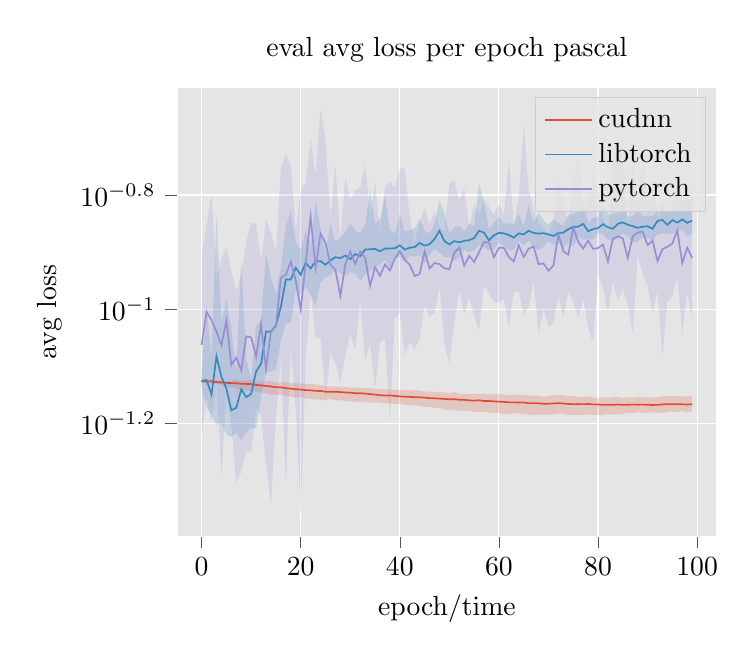
\begin{tikzpicture}

\definecolor{color0}{rgb}{0.886274509803922,0.290196078431373,0.2}
\definecolor{color1}{rgb}{0.203921568627451,0.541176470588235,0.741176470588235}
\definecolor{color2}{rgb}{0.596078431372549,0.556862745098039,0.835294117647059}

\begin{axis}[
axis background/.style={fill=white!89.8039215686275!black},
axis line style={white},
legend cell align={left},
legend style={fill opacity=0.8, draw opacity=1, text opacity=1, draw=white!80!black, fill=white!89.8039215686275!black},
log basis y={10},
tick align=outside,
tick pos=left,
title={eval avg loss per epoch pascal},
x grid style={white},
xlabel={epoch/time},
xmajorgrids,
xmin=-4.95, xmax=103.95,
xtick style={color=white!33.3333333333333!black},
y grid style={white},
ylabel={avg loss},
ymajorgrids,
ymin=0.0401014976380971, ymax=0.244002662318479,
ymode=log,
ytick style={color=white!33.3333333333333!black}
]
\path [fill=color0, fill opacity=0.2, very thin]
(axis cs:0,0.0763048)
--(axis cs:0,0.074306)
--(axis cs:1,0.0741933)
--(axis cs:2,0.0741728)
--(axis cs:3,0.0740423)
--(axis cs:4,0.073857)
--(axis cs:5,0.0732464)
--(axis cs:6,0.0730316)
--(axis cs:7,0.0726815)
--(axis cs:8,0.0722139)
--(axis cs:9,0.072287)
--(axis cs:10,0.0720208)
--(axis cs:11,0.071803)
--(axis cs:12,0.0714627)
--(axis cs:13,0.0713579)
--(axis cs:14,0.0708837)
--(axis cs:15,0.0709141)
--(axis cs:16,0.0707974)
--(axis cs:17,0.070513)
--(axis cs:18,0.0704)
--(axis cs:19,0.0701031)
--(axis cs:20,0.0702514)
--(axis cs:21,0.0698434)
--(axis cs:22,0.0697876)
--(axis cs:23,0.0695003)
--(axis cs:24,0.0694989)
--(axis cs:25,0.0692847)
--(axis cs:26,0.0697221)
--(axis cs:27,0.0693159)
--(axis cs:28,0.0694126)
--(axis cs:29,0.0690623)
--(axis cs:30,0.0690147)
--(axis cs:31,0.0688703)
--(axis cs:32,0.0688074)
--(axis cs:33,0.0690204)
--(axis cs:34,0.0687542)
--(axis cs:35,0.0686813)
--(axis cs:36,0.0686468)
--(axis cs:37,0.0683843)
--(axis cs:38,0.0686145)
--(axis cs:39,0.0683224)
--(axis cs:40,0.0682381)
--(axis cs:41,0.0681189)
--(axis cs:42,0.0678817)
--(axis cs:43,0.0679639)
--(axis cs:44,0.0677241)
--(axis cs:45,0.0674925)
--(axis cs:46,0.0676075)
--(axis cs:47,0.067267)
--(axis cs:48,0.0672767)
--(axis cs:49,0.066735)
--(axis cs:50,0.0667219)
--(axis cs:51,0.0667695)
--(axis cs:52,0.0663634)
--(axis cs:53,0.0664918)
--(axis cs:54,0.0663581)
--(axis cs:55,0.0662017)
--(axis cs:56,0.0661427)
--(axis cs:57,0.0661767)
--(axis cs:58,0.0659616)
--(axis cs:59,0.0658807)
--(axis cs:60,0.0658303)
--(axis cs:61,0.0655401)
--(axis cs:62,0.065609)
--(axis cs:63,0.0658675)
--(axis cs:64,0.0657465)
--(axis cs:65,0.0656359)
--(axis cs:66,0.0654946)
--(axis cs:67,0.0652924)
--(axis cs:68,0.0655354)
--(axis cs:69,0.0653031)
--(axis cs:70,0.0654222)
--(axis cs:71,0.06546)
--(axis cs:72,0.0656585)
--(axis cs:73,0.0656586)
--(axis cs:74,0.0652493)
--(axis cs:75,0.0653743)
--(axis cs:76,0.0653246)
--(axis cs:77,0.0653488)
--(axis cs:78,0.0655542)
--(axis cs:79,0.065304)
--(axis cs:80,0.0653602)
--(axis cs:81,0.0652438)
--(axis cs:82,0.0656778)
--(axis cs:83,0.0653942)
--(axis cs:84,0.0656023)
--(axis cs:85,0.0655714)
--(axis cs:86,0.0659895)
--(axis cs:87,0.0658159)
--(axis cs:88,0.0660952)
--(axis cs:89,0.0658601)
--(axis cs:90,0.0659057)
--(axis cs:91,0.066127)
--(axis cs:92,0.0658867)
--(axis cs:93,0.0659837)
--(axis cs:94,0.0660159)
--(axis cs:95,0.0663029)
--(axis cs:96,0.0660717)
--(axis cs:97,0.0664184)
--(axis cs:98,0.0660986)
--(axis cs:99,0.0664016)
--(axis cs:99,0.0705686)
--(axis cs:99,0.0705686)
--(axis cs:98,0.0704831)
--(axis cs:97,0.0704303)
--(axis cs:96,0.0705127)
--(axis cs:95,0.0705064)
--(axis cs:94,0.0706274)
--(axis cs:93,0.0704812)
--(axis cs:92,0.0701899)
--(axis cs:91,0.0701322)
--(axis cs:90,0.0701429)
--(axis cs:89,0.0701569)
--(axis cs:88,0.0703285)
--(axis cs:87,0.0700578)
--(axis cs:86,0.0702172)
--(axis cs:85,0.0699453)
--(axis cs:84,0.0702719)
--(axis cs:83,0.0702307)
--(axis cs:82,0.069994)
--(axis cs:81,0.0701935)
--(axis cs:80,0.0699727)
--(axis cs:79,0.0701918)
--(axis cs:78,0.070476)
--(axis cs:77,0.0703303)
--(axis cs:76,0.0702431)
--(axis cs:75,0.0706027)
--(axis cs:74,0.0703575)
--(axis cs:73,0.0708758)
--(axis cs:72,0.0706876)
--(axis cs:71,0.070926)
--(axis cs:70,0.0704826)
--(axis cs:69,0.0703829)
--(axis cs:68,0.0706827)
--(axis cs:67,0.0705106)
--(axis cs:66,0.0707178)
--(axis cs:65,0.0708684)
--(axis cs:64,0.0708409)
--(axis cs:63,0.0709945)
--(axis cs:62,0.0707617)
--(axis cs:61,0.0709033)
--(axis cs:60,0.0711634)
--(axis cs:59,0.0709829)
--(axis cs:58,0.0711046)
--(axis cs:57,0.0711149)
--(axis cs:56,0.0711817)
--(axis cs:55,0.0711317)
--(axis cs:54,0.0711012)
--(axis cs:53,0.0711672)
--(axis cs:52,0.0711282)
--(axis cs:51,0.0717023)
--(axis cs:50,0.0714589)
--(axis cs:49,0.0714704)
--(axis cs:48,0.0717452)
--(axis cs:47,0.0717458)
--(axis cs:46,0.0718299)
--(axis cs:45,0.0717848)
--(axis cs:44,0.0721902)
--(axis cs:43,0.0721043)
--(axis cs:42,0.0723391)
--(axis cs:41,0.0721041)
--(axis cs:40,0.0722506)
--(axis cs:39,0.0723223)
--(axis cs:38,0.0723575)
--(axis cs:37,0.0725395)
--(axis cs:36,0.0725224)
--(axis cs:35,0.0726538)
--(axis cs:34,0.0728941)
--(axis cs:33,0.0728202)
--(axis cs:32,0.0728767)
--(axis cs:31,0.0729983)
--(axis cs:30,0.0729806)
--(axis cs:29,0.0731598)
--(axis cs:28,0.0732581)
--(axis cs:27,0.0732024)
--(axis cs:26,0.0733173)
--(axis cs:25,0.073399)
--(axis cs:24,0.0737404)
--(axis cs:23,0.0739099)
--(axis cs:22,0.0740059)
--(axis cs:21,0.0741046)
--(axis cs:20,0.0741708)
--(axis cs:19,0.0742618)
--(axis cs:18,0.0744029)
--(axis cs:17,0.0745833)
--(axis cs:16,0.0745792)
--(axis cs:15,0.0744602)
--(axis cs:14,0.0750889)
--(axis cs:13,0.0748124)
--(axis cs:12,0.0748146)
--(axis cs:11,0.0747062)
--(axis cs:10,0.075297)
--(axis cs:9,0.0749057)
--(axis cs:8,0.0749895)
--(axis cs:7,0.0754499)
--(axis cs:6,0.0749589)
--(axis cs:5,0.0749191)
--(axis cs:4,0.0749143)
--(axis cs:3,0.075172)
--(axis cs:2,0.0754968)
--(axis cs:1,0.0753319)
--(axis cs:0,0.0763048)
--cycle;

\path [fill=color1, fill opacity=0.2, very thin]
(axis cs:0,0.0776313)
--(axis cs:0,0.072879)
--(axis cs:1,0.0674844)
--(axis cs:2,0.0653099)
--(axis cs:3,0.0627944)
--(axis cs:4,0.0631733)
--(axis cs:5,0.0604662)
--(axis cs:6,0.0597716)
--(axis cs:7,0.0607678)
--(axis cs:8,0.0589129)
--(axis cs:9,0.0611026)
--(axis cs:10,0.061931)
--(axis cs:11,0.0618833)
--(axis cs:12,0.070772)
--(axis cs:13,0.0775089)
--(axis cs:14,0.0779247)
--(axis cs:15,0.078629)
--(axis cs:16,0.0879947)
--(axis cs:17,0.0944946)
--(axis cs:18,0.0946584)
--(axis cs:19,0.10796)
--(axis cs:20,0.106566)
--(axis cs:21,0.109253)
--(axis cs:22,0.105977)
--(axis cs:23,0.101723)
--(axis cs:24,0.111286)
--(axis cs:25,0.113862)
--(axis cs:26,0.114786)
--(axis cs:27,0.117061)
--(axis cs:28,0.115892)
--(axis cs:29,0.114617)
--(axis cs:30,0.116262)
--(axis cs:31,0.115455)
--(axis cs:32,0.112137)
--(axis cs:33,0.114976)
--(axis cs:34,0.116774)
--(axis cs:35,0.11776)
--(axis cs:36,0.12)
--(axis cs:37,0.121977)
--(axis cs:38,0.11846)
--(axis cs:39,0.122565)
--(axis cs:40,0.123619)
--(axis cs:41,0.121173)
--(axis cs:42,0.123983)
--(axis cs:43,0.123802)
--(axis cs:44,0.12447)
--(axis cs:45,0.120193)
--(axis cs:46,0.124461)
--(axis cs:47,0.127837)
--(axis cs:48,0.125528)
--(axis cs:49,0.123401)
--(axis cs:50,0.123656)
--(axis cs:51,0.121465)
--(axis cs:52,0.123406)
--(axis cs:53,0.127056)
--(axis cs:54,0.1258)
--(axis cs:55,0.126606)
--(axis cs:56,0.129927)
--(axis cs:57,0.128303)
--(axis cs:58,0.126686)
--(axis cs:59,0.127673)
--(axis cs:60,0.130623)
--(axis cs:61,0.129397)
--(axis cs:62,0.12682)
--(axis cs:63,0.126875)
--(axis cs:64,0.131746)
--(axis cs:65,0.129229)
--(axis cs:66,0.13168)
--(axis cs:67,0.128259)
--(axis cs:68,0.126946)
--(axis cs:69,0.128777)
--(axis cs:70,0.131428)
--(axis cs:71,0.129373)
--(axis cs:72,0.130824)
--(axis cs:73,0.128087)
--(axis cs:74,0.13097)
--(axis cs:75,0.128502)
--(axis cs:76,0.133961)
--(axis cs:77,0.132218)
--(axis cs:78,0.132879)
--(axis cs:79,0.13222)
--(axis cs:80,0.135986)
--(axis cs:81,0.135412)
--(axis cs:82,0.132245)
--(axis cs:83,0.131681)
--(axis cs:84,0.133115)
--(axis cs:85,0.135874)
--(axis cs:86,0.134395)
--(axis cs:87,0.130754)
--(axis cs:88,0.131297)
--(axis cs:89,0.133554)
--(axis cs:90,0.133296)
--(axis cs:91,0.132301)
--(axis cs:92,0.135177)
--(axis cs:93,0.135734)
--(axis cs:94,0.135524)
--(axis cs:95,0.135792)
--(axis cs:96,0.136545)
--(axis cs:97,0.138058)
--(axis cs:98,0.133831)
--(axis cs:99,0.135592)
--(axis cs:99,0.150456)
--(axis cs:99,0.150456)
--(axis cs:98,0.157299)
--(axis cs:97,0.151192)
--(axis cs:96,0.149241)
--(axis cs:95,0.153702)
--(axis cs:94,0.147229)
--(axis cs:93,0.153191)
--(axis cs:92,0.148964)
--(axis cs:91,0.145637)
--(axis cs:90,0.145799)
--(axis cs:89,0.145328)
--(axis cs:88,0.148698)
--(axis cs:87,0.145553)
--(axis cs:86,0.145185)
--(axis cs:85,0.153294)
--(axis cs:84,0.147477)
--(axis cs:83,0.146685)
--(axis cs:82,0.146631)
--(axis cs:81,0.152876)
--(axis cs:80,0.14487)
--(axis cs:79,0.144608)
--(axis cs:78,0.14145)
--(axis cs:77,0.154665)
--(axis cs:76,0.148028)
--(axis cs:75,0.146491)
--(axis cs:74,0.146526)
--(axis cs:73,0.140254)
--(axis cs:72,0.141692)
--(axis cs:71,0.143742)
--(axis cs:70,0.140621)
--(axis cs:69,0.1434)
--(axis cs:68,0.14754)
--(axis cs:67,0.141711)
--(axis cs:66,0.152254)
--(axis cs:65,0.139613)
--(axis cs:64,0.147145)
--(axis cs:63,0.140394)
--(axis cs:62,0.141502)
--(axis cs:61,0.141258)
--(axis cs:60,0.145247)
--(axis cs:59,0.14192)
--(axis cs:58,0.138069)
--(axis cs:57,0.154148)
--(axis cs:56,0.166239)
--(axis cs:55,0.139927)
--(axis cs:54,0.14132)
--(axis cs:53,0.136641)
--(axis cs:52,0.139986)
--(axis cs:51,0.139016)
--(axis cs:50,0.135631)
--(axis cs:49,0.147409)
--(axis cs:48,0.154817)
--(axis cs:47,0.141384)
--(axis cs:46,0.135587)
--(axis cs:45,0.137562)
--(axis cs:44,0.144042)
--(axis cs:43,0.13835)
--(axis cs:42,0.137523)
--(axis cs:41,0.136782)
--(axis cs:40,0.147321)
--(axis cs:39,0.135443)
--(axis cs:38,0.137777)
--(axis cs:37,0.157807)
--(axis cs:36,0.143543)
--(axis cs:35,0.14114)
--(axis cs:34,0.161804)
--(axis cs:33,0.140403)
--(axis cs:32,0.135849)
--(axis cs:31,0.137521)
--(axis cs:30,0.141432)
--(axis cs:29,0.136304)
--(axis cs:28,0.133284)
--(axis cs:27,0.131092)
--(axis cs:26,0.141533)
--(axis cs:25,0.125105)
--(axis cs:24,0.138653)
--(axis cs:23,0.154443)
--(axis cs:22,0.130059)
--(axis cs:21,0.137878)
--(axis cs:20,0.127121)
--(axis cs:19,0.130703)
--(axis cs:18,0.148646)
--(axis cs:17,0.139412)
--(axis cs:16,0.11828)
--(axis cs:15,0.106909)
--(axis cs:14,0.113666)
--(axis cs:13,0.125013)
--(axis cs:12,0.0957994)
--(axis cs:11,0.0935628)
--(axis cs:10,0.075698)
--(axis cs:9,0.081722)
--(axis cs:8,0.122309)
--(axis cs:7,0.0778882)
--(axis cs:6,0.0921429)
--(axis cs:5,0.10444)
--(axis cs:4,0.0948754)
--(axis cs:3,0.146002)
--(axis cs:2,0.0822826)
--(axis cs:1,0.101721)
--(axis cs:0,0.0776313)
--cycle;

\path [fill=color2, fill opacity=0.2, very thin]
(axis cs:0,0.1251995639)
--(axis cs:0,0.0598105138)
--(axis cs:1,0.0702981518)
--(axis cs:2,0.0633538229)
--(axis cs:3,0.0744884569)
--(axis cs:4,0.0509072284)
--(axis cs:5,0.0705281395)
--(axis cs:6,0.0627385779)
--(axis cs:7,0.0497291074)
--(axis cs:8,0.0518793554)
--(axis cs:9,0.0563752627)
--(axis cs:10,0.056338791)
--(axis cs:11,0.0667660289)
--(axis cs:12,0.0651158107)
--(axis cs:13,0.0535107037)
--(axis cs:14,0.0453654876)
--(axis cs:15,0.0646305747)
--(axis cs:16,0.0816814262)
--(axis cs:17,0.0496607745)
--(axis cs:18,0.0850914382)
--(axis cs:19,0.0672796944)
--(axis cs:20,0.0435318968)
--(axis cs:21,0.0811232304)
--(axis cs:22,0.1064643059)
--(axis cs:23,0.0894235118)
--(axis cs:24,0.0887255846)
--(axis cs:25,0.0699467472)
--(axis cs:26,0.0834384767)
--(axis cs:27,0.0804337092)
--(axis cs:28,0.0744777956)
--(axis cs:29,0.083125968)
--(axis cs:30,0.0905108602)
--(axis cs:31,0.0852252966)
--(axis cs:32,0.1035292356)
--(axis cs:33,0.0812223135)
--(axis cs:34,0.0871615007)
--(axis cs:35,0.0723944611)
--(axis cs:36,0.0873688912)
--(axis cs:37,0.0889581851)
--(axis cs:38,0.0636804632)
--(axis cs:39,0.0963433423)
--(axis cs:40,0.0987352811)
--(axis cs:41,0.0830663281)
--(axis cs:42,0.08767304)
--(axis cs:43,0.0850983858)
--(axis cs:44,0.0887169297)
--(axis cs:45,0.1012121662)
--(axis cs:46,0.0971909724)
--(axis cs:47,0.098792186)
--(axis cs:48,0.1093011861)
--(axis cs:49,0.0870002921)
--(axis cs:50,0.0803462708)
--(axis cs:51,0.0950443899)
--(axis cs:52,0.1076677735)
--(axis cs:53,0.0980120687)
--(axis cs:54,0.1051356141)
--(axis cs:55,0.0975622075)
--(axis cs:56,0.0917544748)
--(axis cs:57,0.1102256753)
--(axis cs:58,0.1068369244)
--(axis cs:59,0.1028136745)
--(axis cs:60,0.1026140021)
--(axis cs:61,0.1043353851)
--(axis cs:62,0.092932914)
--(axis cs:63,0.1071914134)
--(axis cs:64,0.1074809429)
--(axis cs:65,0.0979875043)
--(axis cs:66,0.1009229204)
--(axis cs:67,0.1120017534)
--(axis cs:68,0.0908997285)
--(axis cs:69,0.1002152106)
--(axis cs:70,0.0930624553)
--(axis cs:71,0.094723347)
--(axis cs:72,0.1055330429)
--(axis cs:73,0.0970646428)
--(axis cs:74,0.1072683804)
--(axis cs:75,0.1031177828)
--(axis cs:76,0.0967396146)
--(axis cs:77,0.1040080435)
--(axis cs:78,0.0928178142)
--(axis cs:79,0.0873207241)
--(axis cs:80,0.1144324321)
--(axis cs:81,0.1092707362)
--(axis cs:82,0.0990699191)
--(axis cs:83,0.1115053139)
--(axis cs:84,0.1033265941)
--(axis cs:85,0.1087249446)
--(axis cs:86,0.1017762016)
--(axis cs:87,0.0909622937)
--(axis cs:88,0.1244084465)
--(axis cs:89,0.1148451535)
--(axis cs:90,0.1100523204)
--(axis cs:91,0.0984751833)
--(axis cs:92,0.107523062)
--(axis cs:93,0.0828359699)
--(axis cs:94,0.1030719897)
--(axis cs:95,0.1052666428)
--(axis cs:96,0.1146595638)
--(axis cs:97,0.090855545)
--(axis cs:98,0.1073401658)
--(axis cs:99,0.0952692027)
--(axis cs:99,0.1653216861)
--(axis cs:99,0.1653216861)
--(axis cs:98,0.1512831392)
--(axis cs:97,0.1569802477)
--(axis cs:96,0.1695080572)
--(axis cs:95,0.1474820001)
--(axis cs:94,0.149474026)
--(axis cs:93,0.1484766003)
--(axis cs:92,0.1448309001)
--(axis cs:91,0.1674749459)
--(axis cs:90,0.1499902322)
--(axis cs:89,0.1862420209)
--(axis cs:88,0.1511673405)
--(axis cs:87,0.1821400538)
--(axis cs:86,0.140564665)
--(axis cs:85,0.182870231)
--(axis cs:84,0.1950164631)
--(axis cs:83,0.1783776463)
--(axis cs:82,0.136303135)
--(axis cs:81,0.1451914195)
--(axis cs:80,0.1606124358)
--(axis cs:79,0.1708915865)
--(axis cs:78,0.1549806544)
--(axis cs:77,0.1502196009)
--(axis cs:76,0.1847894373)
--(axis cs:75,0.1682672103)
--(axis cs:74,0.1410657063)
--(axis cs:73,0.1560376978)
--(axis cs:72,0.1681705073)
--(axis cs:71,0.1438176172)
--(axis cs:70,0.1354282235)
--(axis cs:69,0.138558344)
--(axis cs:68,0.1422289954)
--(axis cs:67,0.1498897344)
--(axis cs:66,0.1623062244)
--(axis cs:65,0.2105566963)
--(axis cs:64,0.1580182804)
--(axis cs:63,0.1410204383)
--(axis cs:62,0.1821476229)
--(axis cs:61,0.1463445014)
--(axis cs:60,0.152920326)
--(axis cs:59,0.1464541368)
--(axis cs:58,0.1510553772)
--(axis cs:57,0.1551690369)
--(axis cs:56,0.1461733666)
--(axis cs:55,0.1529875127)
--(axis cs:54,0.1388608431)
--(axis cs:53,0.1630636559)
--(axis cs:52,0.1551297002)
--(axis cs:51,0.1681158328)
--(axis cs:50,0.1659286352)
--(axis cs:49,0.1369331752)
--(axis cs:48,0.1398438145)
--(axis cs:47,0.1478500486)
--(axis cs:46,0.1411062112)
--(axis cs:45,0.1506464129)
--(axis cs:44,0.1421200172)
--(axis cs:43,0.1306338408)
--(axis cs:42,0.145419366)
--(axis cs:41,0.1763371702)
--(axis cs:40,0.1764712073)
--(axis cs:39,0.1630730424)
--(axis cs:38,0.1670320234)
--(axis cs:37,0.1643070298)
--(axis cs:36,0.1370965971)
--(axis cs:35,0.1678372145)
--(axis cs:34,0.1458351464)
--(axis cs:33,0.1799693455)
--(axis cs:32,0.1630580583)
--(axis cs:31,0.1615297347)
--(axis cs:30,0.1558029563)
--(axis cs:29,0.170151886)
--(axis cs:28,0.1326437383)
--(axis cs:27,0.1794782472)
--(axis cs:26,0.1449060239)
--(axis cs:25,0.1983689394)
--(axis cs:24,0.2247747722)
--(axis cs:23,0.1714143718)
--(axis cs:22,0.1989115074)
--(axis cs:21,0.1661376744)
--(axis cs:20,0.1618190422)
--(axis cs:19,0.138643496)
--(axis cs:18,0.1776840427)
--(axis cs:17,0.1880502968)
--(axis cs:16,0.1757270025)
--(axis cs:15,0.1260174817)
--(axis cs:14,0.1366353838)
--(axis cs:13,0.1434530167)
--(axis cs:12,0.1216412307)
--(axis cs:11,0.1411757388)
--(axis cs:10,0.1415486688)
--(axis cs:9,0.1312158662)
--(axis cs:8,0.1151236844)
--(axis cs:7,0.1080023267)
--(axis cs:6,0.1166824008)
--(axis cs:5,0.1288204475)
--(axis cs:4,0.122523585)
--(axis cs:3,0.1141009891)
--(axis cs:2,0.1586757575)
--(axis cs:1,0.1398330519)
--(axis cs:0,0.1251995639)
--cycle;

\addplot [semithick, color0]
table {%
0 0.0750162452459335
1 0.07480838149786
2 0.0748418793082237
3 0.0746232494711876
4 0.0745255202054977
5 0.0743761956691742
7 0.0742463693022728
8 0.0741018727421761
10 0.0740136280655861
11 0.0737641230225563
12 0.0736539736390114
15 0.0731059983372688
16 0.07307168841362
17 0.0728077292442322
19 0.0725081562995911
21 0.0722461491823196
22 0.072155699133873
23 0.0720088109374046
24 0.0719877257943153
25 0.0717687606811523
26 0.0717334896326065
27 0.0717698037624359
29 0.071551077067852
30 0.0714892372488976
31 0.071318231523037
32 0.0713325440883636
33 0.0712283179163933
36 0.0707809999585152
37 0.0706641003489494
38 0.0707004740834236
40 0.070426769554615
41 0.0703292340040207
42 0.0703056529164314
43 0.0701833888888359
44 0.0701665505766869
45 0.0700877830386162
46 0.0699364617466927
47 0.0698905810713768
50 0.0696290135383606
51 0.0696465224027634
52 0.0694858953356743
53 0.0694557651877403
54 0.0693074092268944
55 0.0692230090498924
56 0.0693538412451744
57 0.0691204816102982
58 0.069126196205616
61 0.0688832178711891
62 0.0687619373202324
65 0.0687080174684525
66 0.0685300827026367
67 0.0685477629303932
69 0.0683814063668251
70 0.0683815777301788
72 0.0685310363769531
73 0.0684501081705093
74 0.0682937130331993
75 0.0682642012834549
76 0.0682868361473083
77 0.0682530850172043
78 0.0683167949318886
79 0.0681943446397781
80 0.0681710988283157
81 0.068072609603405
83 0.0680704042315483
84 0.0681586340069771
85 0.0680494830012321
87 0.0681434273719788
88 0.0681103616952896
89 0.0681382641196251
90 0.0681052207946777
91 0.0680251643061638
92 0.0680870562791824
93 0.0682016387581825
94 0.0682708323001862
95 0.0682312995195389
96 0.0682618021965027
98 0.0681649968028069
99 0.0682864412665367
};
\addlegendentry{cudnn}
\addplot [semithick, color1]
table {%
0 0.0748142525553703
1 0.0752614140510559
2 0.0709724202752113
3 0.0827635154128075
4 0.0761957615613937
5 0.0726968944072723
6 0.0665895715355873
7 0.0672960504889488
8 0.0724519714713097
9 0.0702114999294281
10 0.0711560696363449
11 0.0778674110770226
12 0.0802848115563393
13 0.0914390981197357
14 0.0913663357496262
15 0.0938323065638542
16 0.101073704659939
17 0.112818256020546
18 0.112757638096809
19 0.11820150911808
20 0.11493718624115
21 0.120620802044868
22 0.11785938590765
23 0.121241100132465
24 0.121408082544804
25 0.119684517383575
26 0.121717900037766
27 0.123409107327461
28 0.122889623045921
29 0.124179780483246
30 0.122439317405224
31 0.12494408339262
32 0.123895078897476
33 0.127248078584671
35 0.127552315592766
36 0.126298785209656
37 0.127724796533585
39 0.127887606620789
40 0.129406586289406
41 0.127203300595284
42 0.128169372677803
43 0.128470882773399
44 0.130701273679733
45 0.129265278577805
46 0.129980012774467
47 0.132789194583893
48 0.137228935956955
49 0.1315858066082
50 0.129903897643089
51 0.131632119417191
52 0.131023585796356
53 0.13176392018795
54 0.132123917341232
55 0.133302807807922
56 0.137266308069229
57 0.136188223958015
58 0.132027700543404
59 0.134707614779472
60 0.136141419410706
61 0.135792091488838
62 0.134937882423401
63 0.133462801575661
64 0.135814681649208
65 0.135195910930634
66 0.137226223945618
67 0.136096805334091
68 0.135679572820663
69 0.135918512940407
70 0.135262683033943
71 0.134360417723656
72 0.136043399572372
73 0.136226430535316
74 0.13814452290535
75 0.139352291822433
76 0.139496996998787
77 0.141090497374535
78 0.137003183364868
79 0.138143107295036
80 0.138728484511375
81 0.140920698642731
82 0.139194294810295
83 0.138368427753448
84 0.14110791683197
85 0.14193557202816
86 0.140593722462654
87 0.139801397919655
88 0.138875097036362
89 0.139471426606178
90 0.139748796820641
91 0.138313889503479
92 0.142760798335075
93 0.143382579088211
94 0.140537068247795
95 0.143260821700096
96 0.141812831163406
97 0.143658697605133
98 0.141683489084244
99 0.14300411939621
};
\addlegendentry{libtorch}
\addplot [semithick, color2]
table {%
0 0.086666651070118
1 0.0990347787737846
2 0.0958111882209778
3 0.0913892164826393
4 0.0865319445729256
5 0.0955604091286659
6 0.0799425095319748
7 0.0823009163141251
8 0.0782411098480225
9 0.0896597430109978
10 0.0893426835536957
11 0.0826596468687057
12 0.094211034476757
13 0.0786996185779572
14 0.0915572643280029
15 0.0933080464601517
16 0.113654144108295
17 0.114851154386997
18 0.121286138892174
19 0.112376533448696
20 0.0999639630317688
21 0.120333924889565
22 0.145273610949516
23 0.118104666471481
24 0.135710343718529
25 0.130694672465324
26 0.119701735675335
27 0.117323189973831
28 0.105601817369461
29 0.119902789592743
30 0.126269042491913
31 0.120075538754463
32 0.126194417476654
33 0.123037457466125
34 0.109803885221481
35 0.118464082479477
36 0.114459522068501
37 0.119891993701458
38 0.116995684802532
39 0.122587151825428
40 0.126367628574371
41 0.122043110430241
42 0.119712509214878
43 0.114358931779861
44 0.115312002599239
45 0.126365095376968
46 0.117865465581417
47 0.120499052107334
48 0.119995966553688
49 0.11794301122427
50 0.117612481117249
51 0.125550672411919
52 0.128333985805511
53 0.119261309504509
54 0.12401919811964
55 0.121059134602547
56 0.126001209020615
57 0.131232142448425
58 0.13081419467926
59 0.123355194926262
60 0.128117501735687
61 0.128119990229607
62 0.123509213328362
63 0.121332451701164
64 0.12945020198822
65 0.123508602380753
66 0.127663314342499
67 0.128786772489548
68 0.119940742850304
69 0.12030066549778
70 0.11682191491127
71 0.119293302297592
72 0.135402470827103
73 0.126378685235977
74 0.124627180397511
75 0.138959527015686
76 0.131367042660713
77 0.127714172005653
78 0.131907299160957
79 0.127585679292679
80 0.128016084432602
81 0.129840090870857
82 0.121224962174892
83 0.132886588573456
84 0.13420943915844
85 0.133039981126785
86 0.122945763170719
87 0.134227856993675
88 0.136249914765358
89 0.136796355247498
90 0.129464462399483
91 0.131995171308517
92 0.121452979743481
93 0.127416461706161
94 0.128716051578522
95 0.130388677120209
96 0.137480556964874
97 0.120412826538086
98 0.128234371542931
99 0.122887663543224
};
\addlegendentry{pytorch}
\end{axis}

\end{tikzpicture}

    \end{figure}
    

    \begin{figure}
        \begin{tikzpicture}[
    axisbg/.style={
        fill=#1!50,
        nearly transparent
    },
    declare function={
      ticklen=0.15;
      xmax=5;
      ymax=5;
      zmax=5;
    },
]






    \begin{axis}[%
        axis background/.style={fill=white!89.8039215686275!black},
        title={},
        grid=major,
        width=12cm,height=12cm,
        xlabel={batch size},
        ylabel={resolution},
        zlabel={time [ms]},
%        legend style={
%            mark size=5,
%            legend cell align=left
%        },
%        legend entries={
%            cuDNN, LibTorch, PyTorch, TorchScript
%        },
        label style={font=\scriptsize},
        ticklabel style={font=\scriptsize},
        view={40}{30},
        xmode=log,
        ymode=log,
        log basis x={2},
        log basis y={2},
        zmode=log,
        log origin=infty
    ]
        \addplot3 [
            opacity=0.7,
            ycomb,
            line width=0.5pt,
            mark=cube*,
            mark size=3,
            fill=cudnn
        ]
        file{./figures/plots/cudnn_train_avg_sample_time.csv};

        \addplot3 [
            opacity=0.7,
            ycomb,
            line width=0.5pt,
            mark=ball,
            mark size=3,
            fill=libtorch,
        ]
        file{./figures/plots/libtorch_train_avg_sample_time.csv};

        \addplot3 [
            opacity=0.7,
            ycomb,
            line width=0.5pt,
            mark=diamond*,
            mark size=3,
            fill=pytorch,
        ]
        file{./figures/plots/pytorch_train_avg_sample_time.csv};

    \end{axis}
\end{tikzpicture}
    \end{figure}
    

    \begin{figure}
        \input{figures/plots/train_avg_used_mem.tex}
    \end{figure}


    \begin{figure}
        \input{figures/plots/train_avg_gpu_util.tex}
    \end{figure}


    \begin{figure}
        \input{figures/plots/eval_avg_sample_time.tex}
    \end{figure}


    \begin{figure}
        \begin{tikzpicture}[
    axisbg/.style={
        fill=#1!50,
        nearly transparent
    },
    declare function={
      ticklen=0.15;
      xmax=5;
      ymax=5;
      zmax=5;
    },
]






    \begin{axis}[%
        axis background/.style={fill=white!89.8039215686275!black},
        title={},
        grid=major,
        width=12cm,height=12cm,
        xlabel={batch size},
        ylabel={resolution},
        zlabel={memory (MB)},
        legend style={
            mark size=5,
            legend cell align=left
        },
        legend entries={
            cuDNN, LibTorch, PyTorch, TorchScript
        },
        label style={font=\scriptsize},
        ticklabel style={font=\scriptsize},
        view={40}{30},
        xmode=log,
        ymode=log,
        log basis x={2},
        log basis y={2},
        zmode=log,
        log origin=infty
    ]
        \addplot3 [
            opacity=0.7,
            ycomb,
            line width=0.5pt,
            mark=cube*,
            mark size=3,
            fill=cudnn
        ]
        file{./figures/plots/cudnn_eval_avg_used_mem.csv};

        \addplot3 [
            opacity=0.7,
            ycomb,
            line width=0.5pt,
            mark=ball,
            mark size=3,
            fill=libtorch,
        ]
        file{./figures/plots/libtorch_eval_avg_used_mem.csv};

        \addplot3 [
            opacity=0.7,
            ycomb,
            line width=0.5pt,
            mark=diamond*,
            mark size=3,
            fill=pytorch,
        ]
        file{./figures/plots/pytorch_eval_avg_used_mem.csv};

        \addplot3 [
            opacity=0.7,
            ycomb,
            line width=0.5pt,
            mark=triangle*,
            mark size=3,
            fill=torchscript,
        ]
        file{./figures/plots/torchscript_eval_avg_used_mem.csv};
    \end{axis}
\end{tikzpicture}
    \end{figure}


    \begin{figure}
        \input{figures/plots/eval_avg_gpu_util.tex}
    \end{figure}


    \begin{figure}
        % This file was created by tikzplotlib v0.9.5.
\begin{tikzpicture}







\begin{axis}[
axis background/.style={fill=white!89.8039215686275!black},
axis line style={white},
legend cell align={left},
legend style={fill opacity=0.8, draw opacity=1, text opacity=1, at={(0.03,0.97)}, anchor=north west, draw=white!80!black, fill=white!89.8039215686275!black},
log basis y={10},
tick align=outside,
tick pos=left,
title={Average sample time for batch size $=32$},
x grid style={white},
xlabel={resolution},
xmajorgrids,
xmin=2.65, xmax=10.35,
xtick style={color=white!33.3333333333333!black},
y grid style={white},
ylabel={time (ms)},
ymajorgrids,
ymin=0.152640394088257, ymax=27.8442975883733,
ymode=log,
ytick style={color=white!33.3333333333333!black},
xticklabels={$2^3$, $2^4$, $2^5$, $2^6$, $2^7$, $2^8$, $2^9$, $2^{10}$},
xtick={3,...,10},
]
\path [fill=cudnn, fill opacity=0.2, very thin]
(axis cs:3,0.201026)
--(axis cs:3,0.19947)
--(axis cs:4,0.199807)
--(axis cs:5,0.227339)
--(axis cs:6,0.330417)
--(axis cs:7,0.861158)
--(axis cs:8,2.71924)
--(axis cs:8,2.77216)
--(axis cs:8,2.77216)
--(axis cs:7,0.88903)
--(axis cs:6,0.3433)
--(axis cs:5,0.230137)
--(axis cs:4,0.204628)
--(axis cs:3,0.201026)
--cycle;

\path [fill=libtorch, fill opacity=0.2, very thin]
(axis cs:3,0.239017)
--(axis cs:3,0.224985)
--(axis cs:4,0.223488)
--(axis cs:5,0.227935)
--(axis cs:6,0.260423)
--(axis cs:7,0.475671)
--(axis cs:8,1.50341)
--(axis cs:9,5.67418)
--(axis cs:9,5.86691)
--(axis cs:9,5.86691)
--(axis cs:8,1.56544)
--(axis cs:7,0.483492)
--(axis cs:6,0.261208)
--(axis cs:5,0.242581)
--(axis cs:4,0.238601)
--(axis cs:3,0.239017)
--cycle;

\path [fill=pytorch, fill opacity=0.2, very thin]
(axis cs:3,1.264947)
--(axis cs:3,1.21564)
--(axis cs:4,1.213545)
--(axis cs:5,1.215587)
--(axis cs:6,1.220171)
--(axis cs:7,1.296469)
--(axis cs:8,2.795173)
--(axis cs:9,9.585992)
--(axis cs:9,9.846071)
--(axis cs:9,9.846071)
--(axis cs:8,2.891976)
--(axis cs:7,1.341868)
--(axis cs:6,1.291262)
--(axis cs:5,1.29437)
--(axis cs:4,1.259168)
--(axis cs:3,1.264947)
--cycle;

\path [fill=white!46.6666666666667!black, fill opacity=0.2, very thin]
(axis cs:3,0.353049)
--(axis cs:3,0.199058)
--(axis cs:4,0.193395)
--(axis cs:5,0.195655)
--(axis cs:6,0.227985)
--(axis cs:7,0.435408)
--(axis cs:8,1.42414)
--(axis cs:9,5.45931)
--(axis cs:10,20.8873)
--(axis cs:10,21.9766)
--(axis cs:10,21.9766)
--(axis cs:9,5.7139)
--(axis cs:8,1.5859)
--(axis cs:7,0.616575)
--(axis cs:6,0.401246)
--(axis cs:5,0.348112)
--(axis cs:4,0.374466)
--(axis cs:3,0.353049)
--cycle;

\path [fill=torchscript, fill opacity=0.2, very thin]
(axis cs:3,0.353049)
--(axis cs:3,0.199058)
--(axis cs:4,0.193395)
--(axis cs:5,0.195655)
--(axis cs:6,0.227985)
--(axis cs:7,0.435408)
--(axis cs:8,1.42414)
--(axis cs:9,5.45931)
--(axis cs:10,20.8873)
--(axis cs:10,21.9766)
--(axis cs:10,21.9766)
--(axis cs:9,5.7139)
--(axis cs:8,1.5859)
--(axis cs:7,0.616575)
--(axis cs:6,0.401246)
--(axis cs:5,0.348112)
--(axis cs:4,0.374466)
--(axis cs:3,0.353049)
--cycle;

\addplot [semithick, cudnn]
table {%
3 0.200238913297653
4 0.202598989009857
5 0.229123681783676
6 0.338942557573318
7 0.870264947414398
8 2.73578190803528
};
\addlegendentry{cudnn}
\addplot [semithick, libtorch]
table {%
3 0.232446998357773
4 0.230680495500565
5 0.237425118684769
6 0.260794192552567
7 0.47879546880722
8 1.53802895545959
9 5.7626690864563
};
\addlegendentry{libtorch}
\addplot [semithick, pytorch]
table {%
3 1.23768603801727
4 1.23296797275543
5 1.24600088596344
6 1.25468814373016
7 1.31825852394104
8 2.83480596542358
9 9.69671154022217
};
\addlegendentry{pytorch}
\addplot [semithick, torchscript]
table {%
3 0.220640391111374
4 0.216945394873619
5 0.211528897285461
6 0.245379000902176
7 0.460912704467773
8 1.45570909976959
9 5.53999090194702
10 21.3651218414307
};
\addlegendentry{torchscript}
\end{axis}

\end{tikzpicture}

    \end{figure}


    \begin{figure}
        % This file was created by tikzplotlib v0.9.5.
\begin{tikzpicture}







\begin{axis}[
axis background/.style={fill=white!89.8039215686275!black},
axis line style={white},
%legend cell align={left},
%legend style={fill opacity=0.8, draw opacity=1, text opacity=1, at={(0.03,0.97)}, anchor=north west, draw=white!80!black, fill=white!89.8039215686275!black},
log basis y={10},
tick align=outside,
tick pos=left,
title={Average used memory for batch size $=32$},
x grid style={white},
xlabel={resolution},
xmajorgrids,
xmin=2.65, xmax=10.35,
xtick style={color=white!33.3333333333333!black},
y grid style={white},
ylabel={memory [MB]},
ymajorgrids,
ymin=981.538600682435, ymax=24927.29576095,
ymode=log,
ytick style={color=white!33.3333333333333!black},
xticklabels={$2^3$, $2^4$, $2^5$, $2^6$, $2^7$, $2^8$, $2^9$, $2^{10}$},
xtick={3,...,10},
]
\path [fill=cudnn, fill opacity=0.2, very thin]
(axis cs:3,1137)
--(axis cs:3,1137)
--(axis cs:4,1161)
--(axis cs:5,1291)
--(axis cs:6,1853)
--(axis cs:7,3819)
--(axis cs:8,11683)
--(axis cs:8,11683)
--(axis cs:8,11683)
--(axis cs:7,3819)
--(axis cs:6,1853)
--(axis cs:5,1291)
--(axis cs:4,1161)
--(axis cs:3,1137)
--cycle;

\path [fill=libtorch, fill opacity=0.2, very thin]
(axis cs:3,1559)
--(axis cs:3,1559)
--(axis cs:4,1567)
--(axis cs:5,1613)
--(axis cs:6,1785)
--(axis cs:7,2529)
--(axis cs:8,5591)
--(axis cs:9,18415)
--(axis cs:9,18417)
--(axis cs:9,18417)
--(axis cs:8,5591)
--(axis cs:7,2529)
--(axis cs:6,1785)
--(axis cs:5,1613)
--(axis cs:4,1567)
--(axis cs:3,1559)
--cycle;

\path [fill=pytorch, fill opacity=0.2, very thin]
(axis cs:3,1529)
--(axis cs:3,1529)
--(axis cs:4,1539)
--(axis cs:5,1583)
--(axis cs:6,1799)
--(axis cs:7,2667)
--(axis cs:8,6473)
--(axis cs:9,21519)
--(axis cs:9,21519)
--(axis cs:9,21519)
--(axis cs:8,6473)
--(axis cs:7,2667)
--(axis cs:6,1799)
--(axis cs:5,1583)
--(axis cs:4,1539)
--(axis cs:3,1529)
--cycle;

\path [fill=white!46.6666666666667!black, fill opacity=0.2, very thin]
(axis cs:3,1357)
--(axis cs:3,1357)
--(axis cs:4,1357)
--(axis cs:5,1359)
--(axis cs:6,1379)
--(axis cs:7,1459.02)
--(axis cs:8,1849.85)
--(axis cs:9,3454.26)
--(axis cs:10,9872.04)
--(axis cs:10,9891)
--(axis cs:10,9891)
--(axis cs:9,3459)
--(axis cs:8,1855)
--(axis cs:7,1461)
--(axis cs:6,1379)
--(axis cs:5,1359)
--(axis cs:4,1357)
--(axis cs:3,1357)
--cycle;

\path [fill=torchscript, fill opacity=0.2, very thin]
(axis cs:3,1357)
--(axis cs:3,1357)
--(axis cs:4,1357)
--(axis cs:5,1359)
--(axis cs:6,1379)
--(axis cs:7,1459.02)
--(axis cs:8,1849.85)
--(axis cs:9,3454.26)
--(axis cs:10,9872.04)
--(axis cs:10,9891)
--(axis cs:10,9891)
--(axis cs:9,3459)
--(axis cs:8,1855)
--(axis cs:7,1461)
--(axis cs:6,1379)
--(axis cs:5,1359)
--(axis cs:4,1357)
--(axis cs:3,1357)
--cycle;

\addplot [semithick, cudnn]
table {%
3 1136.99975585938
4 1161
5 1290.99975585938
6 1853
7 3819.00048828125
8 11683.0029296875
};
%\addlegendentry{cudnn}
\addplot [semithick, libtorch]
table {%
3 1558.99975585938
4 1567.00024414062
5 1613.00024414062
6 1784.99975585938
7 2529.00024414062
8 5590.99951171875
9 18416.791015625
};
%\addlegendentry{libtorch}
\addplot [semithick, pytorch]
table {%
3 1529
4 1539.00024414062
5 1583.00036621094
6 1798.99975585938
7 2667
8 6472.998046875
9 21519.01171875
};
%\addlegendentry{pytorch}
\addplot [semithick, torchscript]
table {%
3 1356.99987792969
4 1356.99987792969
5 1359.00012207031
6 1379
7 1460.80187988281
8 1854.48486328125
9 3458.5263671875
10 9889.10546875
};
%\addlegendentry{torchscript}
\end{axis}

\end{tikzpicture}

    \end{figure}


    \begin{figure}
        % This file was created by tikzplotlib v0.9.5.
\begin{tikzpicture}







\begin{axis}[
axis background/.style={fill=white!89.8039215686275!black},
axis line style={white},
legend cell align={left},
legend style={fill opacity=0.8, draw opacity=1, text opacity=1, at={(0.03,0.03)}, anchor=south west, draw=white!80!black, fill=white!89.8039215686275!black},
log basis y={10},
tick align=outside,
tick pos=left,
title={batch size 32 avg gpu util for resolutions},
x grid style={white},
xlabel={resolution},
xmajorgrids,
xmin=2.65, xmax=10.35,
xtick style={color=white!33.3333333333333!black},
y grid style={white},
ylabel={util (\%)},
ymajorgrids,
ymin=1.64468031885378, ymax=121.604179065866,
ymode=log,
ytick style={color=white!33.3333333333333!black},
xticklabels={$2^3$, $2^4$, $2^5$, $2^6$, $2^7$, $2^8$, $2^9$, $2^{10}$},
xtick={3,...,10},
]
\path [fill=cudnn, fill opacity=0.2, very thin]
(axis cs:3,96)
--(axis cs:3,95)
--(axis cs:4,92)
--(axis cs:5,85)
--(axis cs:6,65)
--(axis cs:7,45)
--(axis cs:8,43)
--(axis cs:8,48)
--(axis cs:8,48)
--(axis cs:7,47)
--(axis cs:6,68)
--(axis cs:5,86)
--(axis cs:4,95)
--(axis cs:3,96)
--cycle;

\path [fill=libtorch, fill opacity=0.2, very thin]
(axis cs:3,90)
--(axis cs:3,84)
--(axis cs:4,85)
--(axis cs:5,85)
--(axis cs:6,90)
--(axis cs:7,83)
--(axis cs:8,86)
--(axis cs:9,74)
--(axis cs:9,97)
--(axis cs:9,97)
--(axis cs:8,93)
--(axis cs:7,88)
--(axis cs:6,92)
--(axis cs:5,91)
--(axis cs:4,90)
--(axis cs:3,90)
--cycle;

\path [fill=pytorch, fill opacity=0.2, very thin]
(axis cs:3,21)
--(axis cs:3,6)
--(axis cs:4,7)
--(axis cs:5,7)
--(axis cs:6,8)
--(axis cs:7,12)
--(axis cs:8,20)
--(axis cs:9,60)
--(axis cs:9,100)
--(axis cs:9,100)
--(axis cs:8,39)
--(axis cs:7,18)
--(axis cs:6,15)
--(axis cs:5,19)
--(axis cs:4,15)
--(axis cs:3,21)
--cycle;

\path [fill=white!46.6666666666667!black, fill opacity=0.2, very thin]
(axis cs:3,87)
--(axis cs:3,27)
--(axis cs:4,64)
--(axis cs:5,29)
--(axis cs:6,2)
--(axis cs:7,18)
--(axis cs:8,16)
--(axis cs:9,16)
--(axis cs:10,2)
--(axis cs:10,100)
--(axis cs:10,100)
--(axis cs:9,94)
--(axis cs:8,92)
--(axis cs:7,88)
--(axis cs:6,90)
--(axis cs:5,89)
--(axis cs:4,86)
--(axis cs:3,87)
--cycle;

\path [fill=torchscript, fill opacity=0.2, very thin]
(axis cs:3,87)
--(axis cs:3,27)
--(axis cs:4,64)
--(axis cs:5,29)
--(axis cs:6,2)
--(axis cs:7,18)
--(axis cs:8,16)
--(axis cs:9,16)
--(axis cs:10,2)
--(axis cs:10,100)
--(axis cs:10,100)
--(axis cs:9,94)
--(axis cs:8,92)
--(axis cs:7,88)
--(axis cs:6,90)
--(axis cs:5,89)
--(axis cs:4,86)
--(axis cs:3,87)
--cycle;

\addplot [semithick, cudnn]
table {%
3 95.5999984741211
4 93.5
5 85.4999923706055
6 66.6999893188477
7 46.2000007629395
8 44.7999992370605
};
\addlegendentry{cudnn}
\addplot [semithick, libtorch]
table {%
3 87.0000076293945
4 86.9000015258789
5 87.1999969482422
6 91.3000030517578
7 85.4999923706055
8 89.6000137329102
9 80.3999938964844
};
\addlegendentry{libtorch}
\addplot [semithick, pytorch]
table {%
3 9.05000019073486
4 10.0999994277954
5 11.6499996185303
6 11
7 13.9499988555908
8 32.6999969482422
9 84.0500106811523
};
\addlegendentry{pytorch}
\addplot [semithick, torchscript]
table {%
3 75.7000045776367
4 81.5999908447266
5 82.6999969482422
6 81.1000061035156
7 78.4000015258789
8 82.5
9 71.0000076293945
10 89.1999969482422
};
\addlegendentry{torchscript}
\end{axis}

\end{tikzpicture}

    \end{figure}


    \begin{figure}
        % This file was created by tikzplotlib v0.9.5.
\begin{tikzpicture}







\begin{axis}[
axis background/.style={fill=white!89.8039215686275!black},
axis line style={white},
%legend cell align={left},
%legend style={fill opacity=0.8, draw opacity=1, text opacity=1, draw=white!80!black, fill=white!89.8039215686275!black},
log basis y={10},
tick align=outside,
tick pos=left,
title={Average sample time for resolution $=64$},
x grid style={white},
xlabel={batch size},
xmajorgrids,
xmin=2.7, xmax=9.3,
xtick style={color=white!33.3333333333333!black},
y grid style={white},
%ylabel={time [ms]},
ymajorgrids,
ymin=0.0318818812180445, ymax=4.24381955156468,
ymode=log,
ytick style={color=white!33.3333333333333!black},
xticklabels={$2^3$, $2^4$, $2^5$, $2^6$, $2^7$, $2^8$, $2^9$},
xtick={3,...,9},
]
\path [fill=cudnn, fill opacity=0.2, very thin]
(axis cs:3,0.532711)
--(axis cs:3,0.525274)
--(axis cs:4,0.325467)
--(axis cs:5,0.227339)
--(axis cs:6,0.137164)
--(axis cs:7,0.127286)
--(axis cs:8,0.107328)
--(axis cs:9,0.0943382)
--(axis cs:9,0.100206)
--(axis cs:9,0.100206)
--(axis cs:8,0.1119)
--(axis cs:7,0.129387)
--(axis cs:6,0.145102)
--(axis cs:5,0.230137)
--(axis cs:4,0.333086)
--(axis cs:3,0.532711)
--cycle;

\path [fill=libtorch, fill opacity=0.2, very thin]
(axis cs:3,0.7206)
--(axis cs:3,0.643425)
--(axis cs:4,0.371694)
--(axis cs:5,0.227935)
--(axis cs:6,0.138768)
--(axis cs:7,0.110285)
--(axis cs:8,0.0866569)
--(axis cs:9,0.0769451)
--(axis cs:9,0.077837)
--(axis cs:9,0.077837)
--(axis cs:8,0.0870269)
--(axis cs:7,0.110558)
--(axis cs:6,0.149246)
--(axis cs:5,0.242581)
--(axis cs:4,0.39549)
--(axis cs:3,0.7206)
--cycle;

\path [fill=pytorch, fill opacity=0.2, very thin]
(axis cs:3,3.397831)
--(axis cs:3,3.123268)
--(axis cs:4,2.145072)
--(axis cs:5,1.215587)
--(axis cs:6,0.90215)
--(axis cs:7,0.489502)
--(axis cs:8,0.516421)
--(axis cs:9,0.290157)
--(axis cs:9,0.314908)
--(axis cs:9,0.314908)
--(axis cs:8,0.564356)
--(axis cs:7,0.522439)
--(axis cs:6,1.003318)
--(axis cs:5,1.29437)
--(axis cs:4,2.273831)
--(axis cs:3,3.397831)
--cycle;

\path [fill=white!46.6666666666667!black, fill opacity=0.2, very thin]
(axis cs:3,0.797093)
--(axis cs:3,0.633669)
--(axis cs:4,0.342584)
--(axis cs:5,0.195655)
--(axis cs:6,0.101828)
--(axis cs:7,0.071068)
--(axis cs:8,0.0474417)
--(axis cs:9,0.0398198)
--(axis cs:9,0.13526)
--(axis cs:9,0.13526)
--(axis cs:8,0.145412)
--(axis cs:7,0.180774)
--(axis cs:6,0.20295)
--(axis cs:5,0.348112)
--(axis cs:4,0.497252)
--(axis cs:3,0.797093)
--cycle;

\path [fill=torchscript, fill opacity=0.2, very thin]
(axis cs:3,0.797093)
--(axis cs:3,0.633669)
--(axis cs:4,0.342584)
--(axis cs:5,0.195655)
--(axis cs:6,0.101828)
--(axis cs:7,0.071068)
--(axis cs:8,0.0474417)
--(axis cs:9,0.0398198)
--(axis cs:9,0.13526)
--(axis cs:9,0.13526)
--(axis cs:8,0.145412)
--(axis cs:7,0.180774)
--(axis cs:6,0.20295)
--(axis cs:5,0.348112)
--(axis cs:4,0.497252)
--(axis cs:3,0.797093)
--cycle;

\addplot [semithick, cudnn]
table {%
3 0.527113080024719
4 0.328776597976685
5 0.229123681783676
6 0.139674320816994
7 0.128557801246643
8 0.10912749171257
9 0.098616324365139
};
%\addlegendentry{cudnn}
\addplot [semithick, libtorch]
table {%
3 0.66579794883728
4 0.376946628093719
5 0.237425118684769
6 0.141885712742805
7 0.110373191535473
8 0.0867782235145569
9 0.077290840446949
};
%\addlegendentry{libtorch}
\addplot [semithick, pytorch]
table {%
3 3.20224666595459
4 2.2035346031189
5 1.24600088596344
6 0.938888311386108
7 0.50709193944931
8 0.551432967185974
9 0.300852745771408
};
%\addlegendentry{pytorch}
\addplot [semithick, torchscript]
table {%
3 0.662334620952606
4 0.360176265239716
5 0.211528897285461
6 0.112016521394253
7 0.0824229493737221
8 0.0573519766330719
9 0.0495683811604977
};
%\addlegendentry{torchscript}
\end{axis}

\end{tikzpicture}

    \end{figure}


    \begin{figure}
        % This file was created by tikzplotlib v0.9.5.
\begin{tikzpicture}







\begin{axis}[
axis background/.style={fill=white!89.8039215686275!black},
axis line style={white},
%legend cell align={left},
%legend style={fill opacity=0.8, draw opacity=1, text opacity=1, at={(0.03,0.97)}, anchor=north west, draw=white!80!black, fill=white!89.8039215686275!black},
log basis y={10},
tick align=outside,
tick pos=left,
title={Average used memory for resolution $=64$},
x grid style={white},
xlabel={batch size},
xmajorgrids,
xmin=2.7, xmax=9.3,
xtick style={color=white!33.3333333333333!black},
y grid style={white},
%ylabel={memory [MB]},
ymajorgrids,
ymin=1000, ymax=4631.40123788891,
ymode=log,
ytick style={color=white!33.3333333333333!black},
xticklabels={$2^3$, $2^4$, $2^5$, $2^6$, $2^7$, $2^8$, $2^9$},
xtick={3,...,9},
]
\path [fill=cudnn, fill opacity=0.2, very thin]
(axis cs:3,1079)
--(axis cs:3,1079)
--(axis cs:4,1163)
--(axis cs:5,1291)
--(axis cs:6,1519)
--(axis cs:7,1961)
--(axis cs:8,2863)
--(axis cs:9,4321)
--(axis cs:9,4321)
--(axis cs:9,4321)
--(axis cs:8,2863)
--(axis cs:7,1961)
--(axis cs:6,1519)
--(axis cs:5,1291)
--(axis cs:4,1163)
--(axis cs:3,1079)
--cycle;

\path [fill=libtorch, fill opacity=0.2, very thin]
(axis cs:3,1551)
--(axis cs:3,1551)
--(axis cs:4,1573)
--(axis cs:5,1613)
--(axis cs:6,1669)
--(axis cs:7,1793)
--(axis cs:8,2105)
--(axis cs:9,2781)
--(axis cs:9,2781)
--(axis cs:9,2781)
--(axis cs:8,2105)
--(axis cs:7,1793)
--(axis cs:6,1669)
--(axis cs:5,1613)
--(axis cs:4,1573)
--(axis cs:3,1551)
--cycle;

\path [fill=pytorch, fill opacity=0.2, very thin]
(axis cs:3,1537)
--(axis cs:3,1537)
--(axis cs:4,1553)
--(axis cs:5,1583)
--(axis cs:6,1655)
--(axis cs:7,1801)
--(axis cs:8,2065)
--(axis cs:9,2621)
--(axis cs:9,2623)
--(axis cs:9,2623)
--(axis cs:8,2065)
--(axis cs:7,1801)
--(axis cs:6,1655)
--(axis cs:5,1583)
--(axis cs:4,1555)
--(axis cs:3,1537)
--cycle;

\path [fill=white!46.6666666666667!black, fill opacity=0.2, very thin]
(axis cs:3,1341)
--(axis cs:3,1341)
--(axis cs:4,1357)
--(axis cs:5,1359)
--(axis cs:6,1403)
--(axis cs:7,1391)
--(axis cs:8,1459.14)
--(axis cs:9,1633)
--(axis cs:9,1919)
--(axis cs:9,1919)
--(axis cs:8,1461)
--(axis cs:7,1391)
--(axis cs:6,1403)
--(axis cs:5,1359)
--(axis cs:4,1357)
--(axis cs:3,1341)
--cycle;

\path [fill=torchscript, fill opacity=0.2, very thin]
(axis cs:3,1341)
--(axis cs:3,1341)
--(axis cs:4,1357)
--(axis cs:5,1359)
--(axis cs:6,1403)
--(axis cs:7,1391)
--(axis cs:8,1459.14)
--(axis cs:9,1633)
--(axis cs:9,1919)
--(axis cs:9,1919)
--(axis cs:8,1461)
--(axis cs:7,1391)
--(axis cs:6,1403)
--(axis cs:5,1359)
--(axis cs:4,1357)
--(axis cs:3,1341)
--cycle;

\addplot [semithick, cudnn]
table {%
3 1079
4 1162.99987792969
5 1290.99975585938
6 1518.99963378906
7 1961.00012207031
8 2863.00073242188
9 4321.0009765625
};
%\addlegendentry{cudnn}
\addplot [semithick, libtorch]
table {%
3 1551.00012207031
4 1573
5 1613.00024414062
6 1669.00048828125
7 1793.00012207031
8 2105.00048828125
9 2781
};
%\addlegendentry{libtorch}
\addplot [semithick, pytorch]
table {%
3 1537
4 1554.19982910156
5 1583.00036621094
6 1654.99975585938
7 1800.99975585938
8 2064.99951171875
9 2621.69946289062
};
%\addlegendentry{pytorch}
\addplot [semithick, torchscript]
table {%
3 1341
4 1356.99987792969
5 1359.00012207031
6 1403.00036621094
7 1391.00036621094
8 1460.81384277344
9 1886.31420898438
};
%\addlegendentry{torchscript}
\end{axis}

\end{tikzpicture}

    \end{figure}


    \begin{figure}
        % This file was created by tikzplotlib v0.9.5.
\begin{tikzpicture}







\begin{axis}[
axis background/.style={fill=white!89.8039215686275!black},
axis line style={white},
legend cell align={left},
legend style={fill opacity=0.8, draw opacity=1, text opacity=1, at={(0.03,0.03)}, anchor=south west, draw=white!80!black, fill=white!89.8039215686275!black},
log basis y={10},
tick align=outside,
tick pos=left,
title={resolution 32 avg gpu util for batch size},
x grid style={white},
xlabel={batch size},
xmajorgrids,
xmin=2.7, xmax=9.3,
xtick style={color=white!33.3333333333333!black},
y grid style={white},
ylabel={util (\%)},
ymajorgrids,
ymin=7.24810179764196e-76, ymax=436822.288427557,
ymode=log,
ytick style={color=white!33.3333333333333!black},
xticklabels={$2^3$, $2^4$, $2^5$, $2^6$, $2^7$, $2^8$, $2^9$},
xtick={3,...,9},
]
\path [fill=cudnn, fill opacity=0.2, very thin]
(axis cs:3,91)
--(axis cs:3,90)
--(axis cs:4,87)
--(axis cs:5,85)
--(axis cs:6,86)
--(axis cs:7,76)
--(axis cs:8,71)
--(axis cs:9,69)
--(axis cs:9,74)
--(axis cs:9,74)
--(axis cs:8,74)
--(axis cs:7,78)
--(axis cs:6,89)
--(axis cs:5,86)
--(axis cs:4,89)
--(axis cs:3,91)
--cycle;

\path [fill=libtorch, fill opacity=0.2, very thin]
(axis cs:3,82)
--(axis cs:3,74)
--(axis cs:4,80)
--(axis cs:5,85)
--(axis cs:6,85)
--(axis cs:7,91)
--(axis cs:8,89)
--(axis cs:9,89)
--(axis cs:9,93)
--(axis cs:9,93)
--(axis cs:8,91)
--(axis cs:7,93)
--(axis cs:6,91)
--(axis cs:5,91)
--(axis cs:4,85)
--(axis cs:3,82)
--cycle;

\path [fill=pytorch, fill opacity=0.2, very thin]
(axis cs:3,35)
--(axis cs:3,25)
--(axis cs:4,13)
--(axis cs:5,7)
--(axis cs:6,7)
--(axis cs:7,9.12835328566328e-71)
--(axis cs:8,1.36815581825213e-71)
--(axis cs:9,5.73048101459414e-71)
--(axis cs:9,20)
--(axis cs:9,20)
--(axis cs:8,10)
--(axis cs:7,10)
--(axis cs:6,11)
--(axis cs:5,19)
--(axis cs:4,22)
--(axis cs:3,35)
--cycle;

\path [fill=white!46.6666666666667!black, fill opacity=0.2, very thin]
(axis cs:3,81)
--(axis cs:3,4.38880587685435e-71)
--(axis cs:4,20)
--(axis cs:5,29)
--(axis cs:6,86)
--(axis cs:7,80)
--(axis cs:8,82)
--(axis cs:9,74)
--(axis cs:9,83)
--(axis cs:9,83)
--(axis cs:8,87)
--(axis cs:7,89)
--(axis cs:6,89)
--(axis cs:5,89)
--(axis cs:4,84)
--(axis cs:3,81)
--cycle;

\path [fill=torchscript, fill opacity=0.2, very thin]
(axis cs:3,81)
--(axis cs:3,3.40444345591596e-72)
--(axis cs:4,20)
--(axis cs:5,29)
--(axis cs:6,86)
--(axis cs:7,80)
--(axis cs:8,82)
--(axis cs:9,74)
--(axis cs:9,83)
--(axis cs:9,83)
--(axis cs:8,87)
--(axis cs:7,89)
--(axis cs:6,89)
--(axis cs:5,89)
--(axis cs:4,84)
--(axis cs:3,81)
--cycle;

\addplot [semithick, cudnn]
table {%
3 90.8000106811523
5 85.4999923706055
6 87.8000106811523
7 76.9999923706055
8 72.7999954223633
9 71.9999923706055
};
\addlegendentry{cudnn}
\addplot [semithick, libtorch]
table {%
3 79.0000076293945
4 83.5999984741211
5 87.1999969482422
7 92.0999984741211
8 89.8000106811523
9 90.9999923706055
};
\addlegendentry{libtorch}
\addplot [semithick, pytorch]
table {%
3 30.2500019073486
4 18.4499988555908
5 11.6499996185303
6 8.34999847412109
7 3.25000023841858
8 2.59999942779541
9 7.5
};
\addlegendentry{pytorch}
\addplot [semithick, torchscript]
table {%
3 70.2999954223633
4 76.6999893188477
5 82.6999969482422
6 88.7000045776367
8 86.4000091552734
9 80.2999954223633
};
\addlegendentry{torchscript}
\end{axis}

\end{tikzpicture}

    \end{figure}

\end{document}